\documentclass[10pt]{report}
\usepackage{graphicx}
\usepackage{varwidth}
\usepackage{enumitem}
\usepackage{amsmath}
\usepackage{pifont}
\usepackage{arydshln}
\usepackage{tikz}
\usepackage{lscape}
\usepackage{bm}
\usepackage{nicefrac}
\usepackage[landscape]{geometry}
\geometry{a4paper, total={282mm,200mm}, left=0mm, top=5mm}
\renewcommand{\labelenumi}{\bfseries(\alph{enumi})\phantom{x}}
\newcommand\omicron{o}
\hfuzz=50pt
\setlist[enumerate]{leftmargin=0pt,itemindent=12pt}
\pagenumbering{gobble}
\begin{document}
\thispagestyle{empty}
\begin{tabular}{c:c}
\begin{minipage}[c][99mm][t]{0.49\linewidth}
\begin{center}
\vspace{7mm}
{\huge Kubická rovnice, skupina \textit{Alpha $\alpha$} -\romannumeral1}\\[4.5mm]
\textit{Meno:}\phantom{xxxxxxxxxxxxxxxxxxxxxxxxxxxxxxxxxxxxxxxxxxxxxxxxxxxxxxxxxxxxxxxxx}\\[3.5mm]
\textbf{Vypočítej součet kořenů kubické rovnice.} Dvojitý kořen považuj do součtu za dva.\\Analogicky pro trojitý kořen. Pokud ti vyjde stejný výsledek jako je za otazníky, tak\\napravo obarvi příslušející kroužek načerno. \textbf{Spolu odevzdejte výsledné slovo}.\\[3mm]
\begin{minipage}{0.77\linewidth}
\begin{center}
\begin{varwidth}{\textwidth}
\begin{enumerate}
\large
\item $3x^3+3x^2-36x=0$\quad \dotfill\; ???\;\dotfill \quad -1
\item $x^3+3x^2-x-3=0$\quad \dotfill\; ???\;\dotfill \quad 1
\item $12x^3-10x^2-64x-42=0$\quad \dotfill\; ???\;\dotfill \quad $\nicefrac{5}{6}$
\item $8x^3-30x^2-14x+24=0$\quad \dotfill\; ???\;\dotfill \quad $\nicefrac{15}{4}$
\item \quad \dotfill\; ???\;\dotfill \quad nebarvi
\item \quad \dotfill\; ???\;\dotfill \quad nebarvi
\end{enumerate}
\end{varwidth}
\end{center}
\end{minipage}
\begin{minipage}{0.20\linewidth}
\begin{center}
{\Huge\bfseries 1.} \\[2mm]
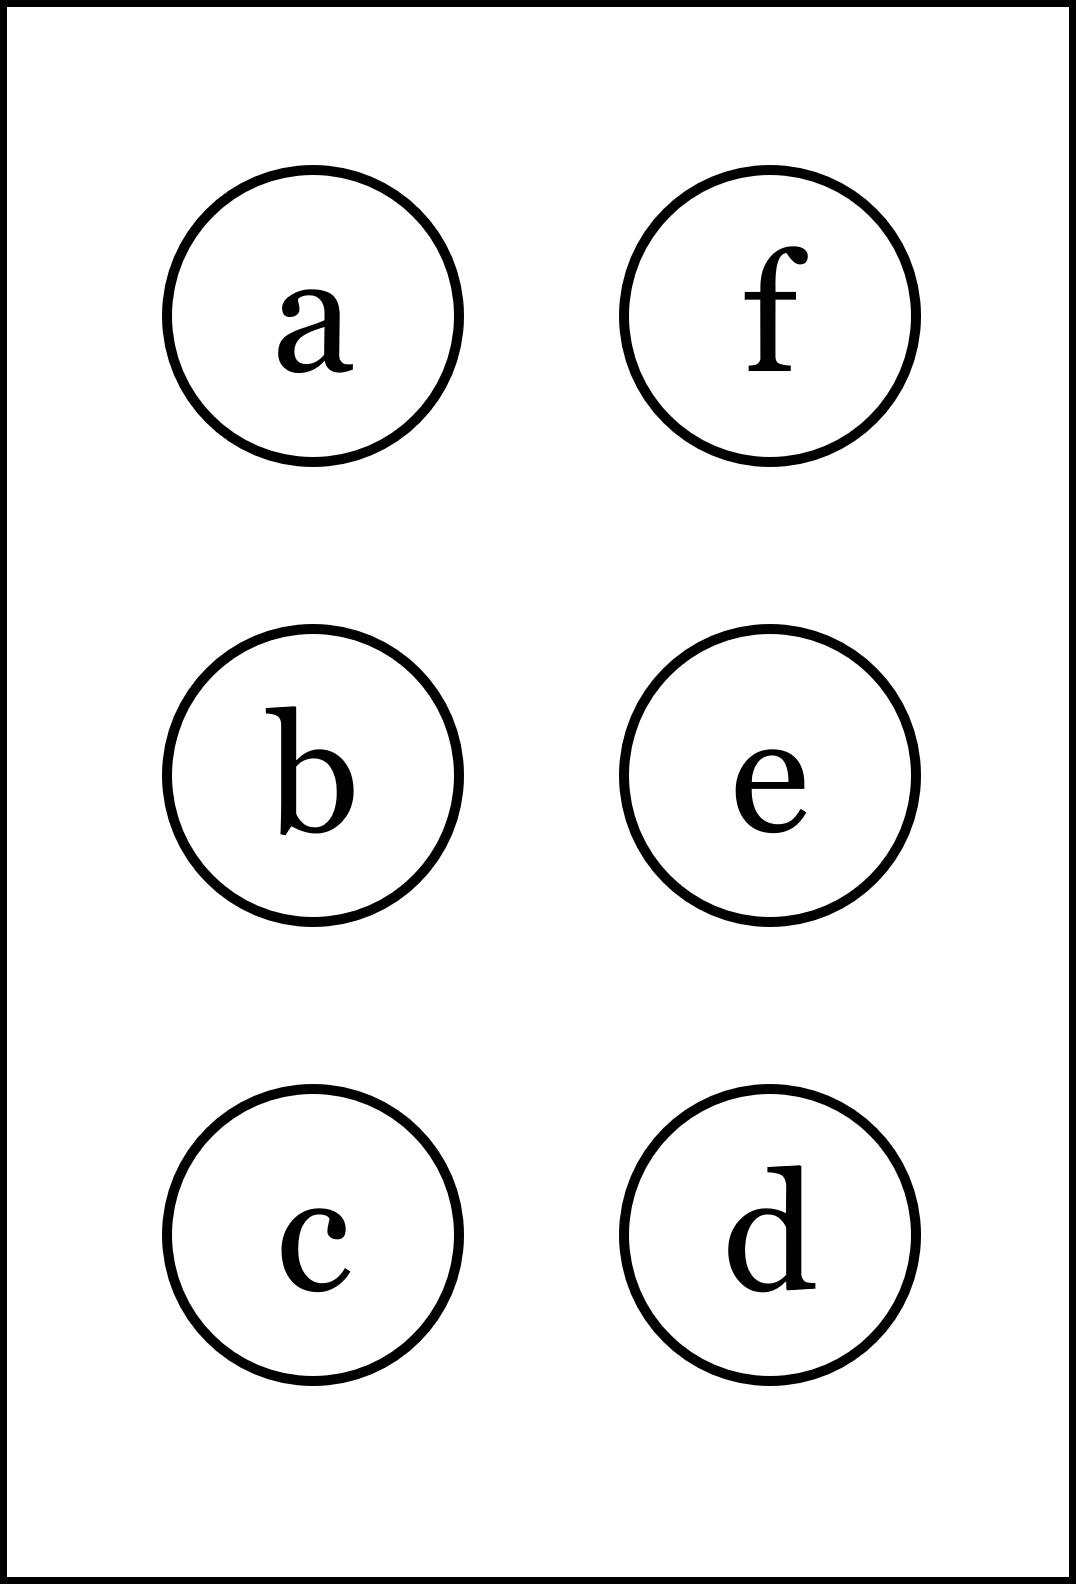
\includegraphics[height=40mm]{../images/braille.png}
{\small Písmeno Braillovej abecedy}
\end{center}
\end{minipage}
\end{center}
\end{minipage}
&
\begin{minipage}[c][99mm][t]{0.49\linewidth}
\begin{center}
\vspace{7mm}
{\huge Kubická rovnice, skupina \textit{Alpha $\alpha$} -\romannumeral2}\\[4.5mm]
\textit{Meno:}\phantom{xxxxxxxxxxxxxxxxxxxxxxxxxxxxxxxxxxxxxxxxxxxxxxxxxxxxxxxxxxxxxxxxx}\\[3.5mm]
\textbf{Vypočítej součet kořenů kubické rovnice.} Dvojitý kořen považuj do součtu za dva.\\Analogicky pro trojitý kořen. Pokud ti vyjde stejný výsledek jako je za otazníky, tak\\napravo obarvi příslušející kroužek načerno. \textbf{Spolu odevzdejte výsledné slovo}.\\[3mm]
\begin{minipage}{0.77\linewidth}
\begin{center}
\begin{varwidth}{\textwidth}
\begin{enumerate}
\large
\item $-2x^3+6x^2-4x=0$\quad \dotfill\; ???\;\dotfill \quad 3
\item $x^3+4x^2-20x-48=0$\quad \dotfill\; ???\;\dotfill \quad 8
\item $8x^3-4x^2-8x+4=0$\quad \dotfill\; ???\;\dotfill \quad $\nicefrac{3}{2}$
\item $-6x^3-3x^2+21x+18=0$\quad \dotfill\; ???\;\dotfill \quad $\nicefrac{5}{2}$
\item \quad \dotfill\; ???\;\dotfill \quad nebarvi
\item \quad \dotfill\; ???\;\dotfill \quad vybarvi
\end{enumerate}
\end{varwidth}
\end{center}
\end{minipage}
\begin{minipage}{0.20\linewidth}
\begin{center}
{\Huge\bfseries 2.} \\[2mm]
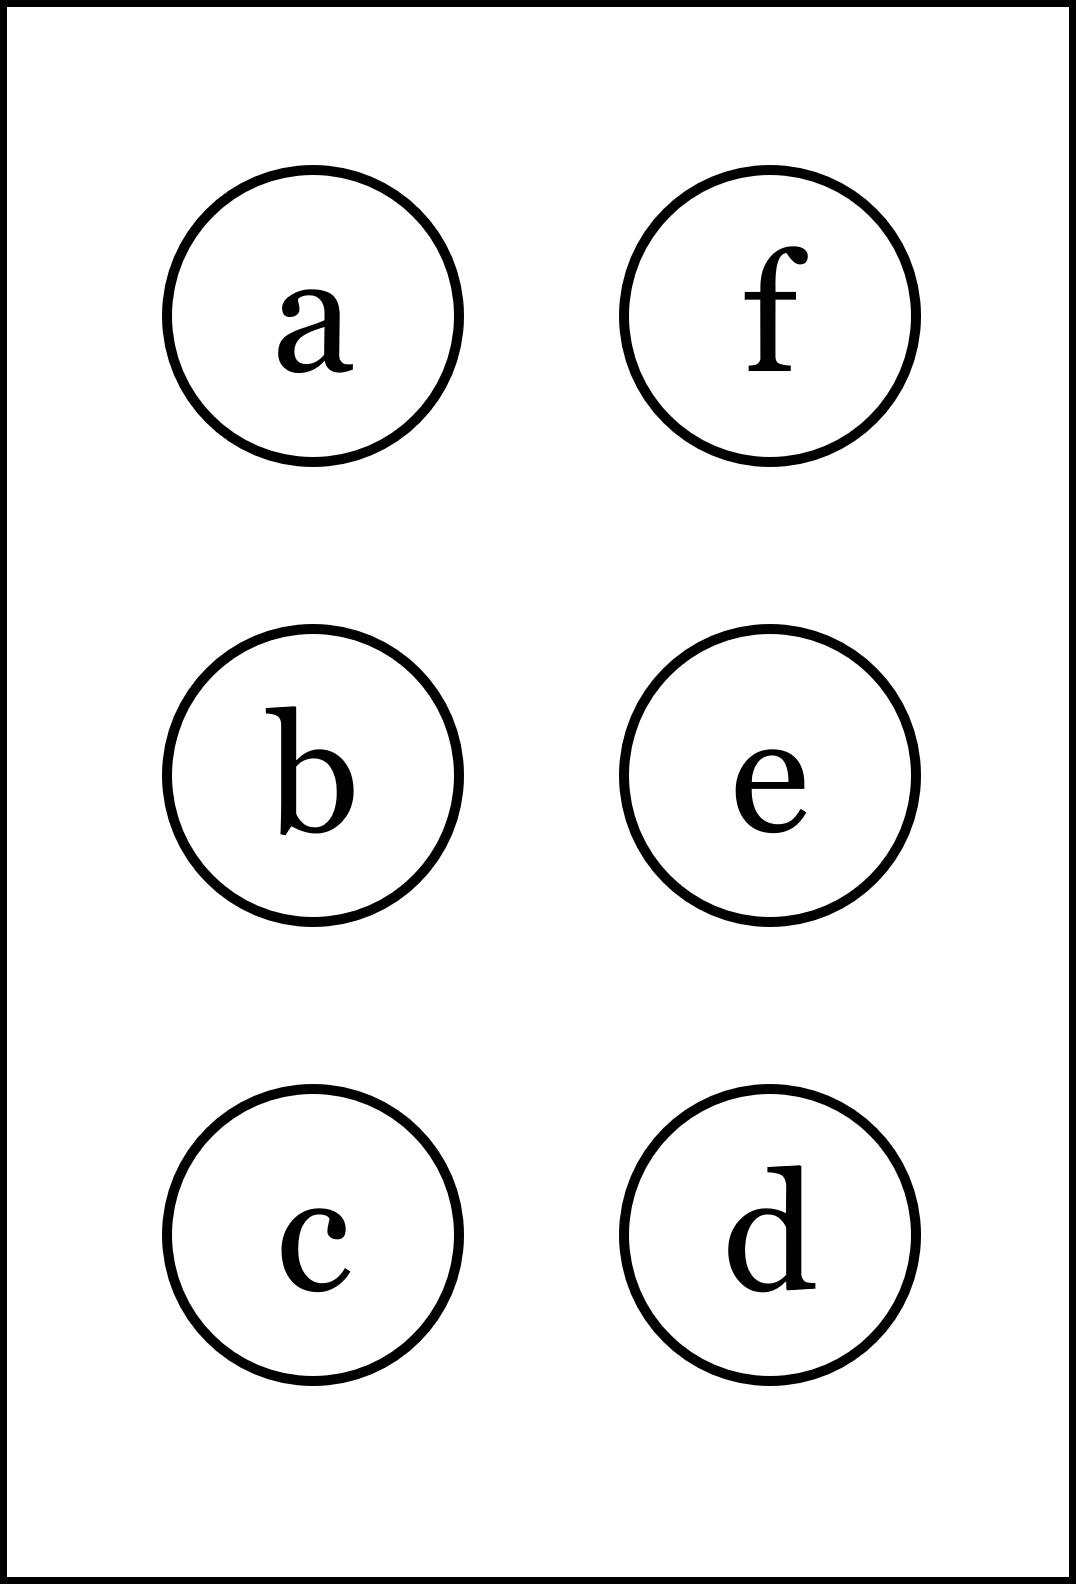
\includegraphics[height=40mm]{../images/braille.png}
{\small Písmeno Braillovej abecedy}
\end{center}
\end{minipage}
\end{center}
\end{minipage}
\\ \hdashline
\begin{minipage}[c][99mm][t]{0.49\linewidth}
\begin{center}
\vspace{7mm}
{\huge Kubická rovnice, skupina \textit{Alpha $\alpha$} -\romannumeral3}\\[4.5mm]
\textit{Meno:}\phantom{xxxxxxxxxxxxxxxxxxxxxxxxxxxxxxxxxxxxxxxxxxxxxxxxxxxxxxxxxxxxxxxxx}\\[3.5mm]
\textbf{Vypočítej součet kořenů kubické rovnice.} Dvojitý kořen považuj do součtu za dva.\\Analogicky pro trojitý kořen. Pokud ti vyjde stejný výsledek jako je za otazníky, tak\\napravo obarvi příslušející kroužek načerno. \textbf{Spolu odevzdejte výsledné slovo}.\\[3mm]
\begin{minipage}{0.77\linewidth}
\begin{center}
\begin{varwidth}{\textwidth}
\begin{enumerate}
\large
\item $2x^3+4x^2-16x=0$\quad \dotfill\; ???\;\dotfill \quad -2
\item $3x^3-21x^2+33x-15=0$\quad \dotfill\; ???\;\dotfill \quad 7
\item $-32x^3+80x^2-64x+16=0$\quad \dotfill\; ???\;\dotfill \quad $\nicefrac{-1}{2}$
\item $-8x^3+16x^2+18x-36=0$\quad \dotfill\; ???\;\dotfill \quad -5
\item \quad \dotfill\; ???\;\dotfill \quad vybarvi
\item \quad \dotfill\; ???\;\dotfill \quad nebarvi
\end{enumerate}
\end{varwidth}
\end{center}
\end{minipage}
\begin{minipage}{0.20\linewidth}
\begin{center}
{\Huge\bfseries 3.} \\[2mm]
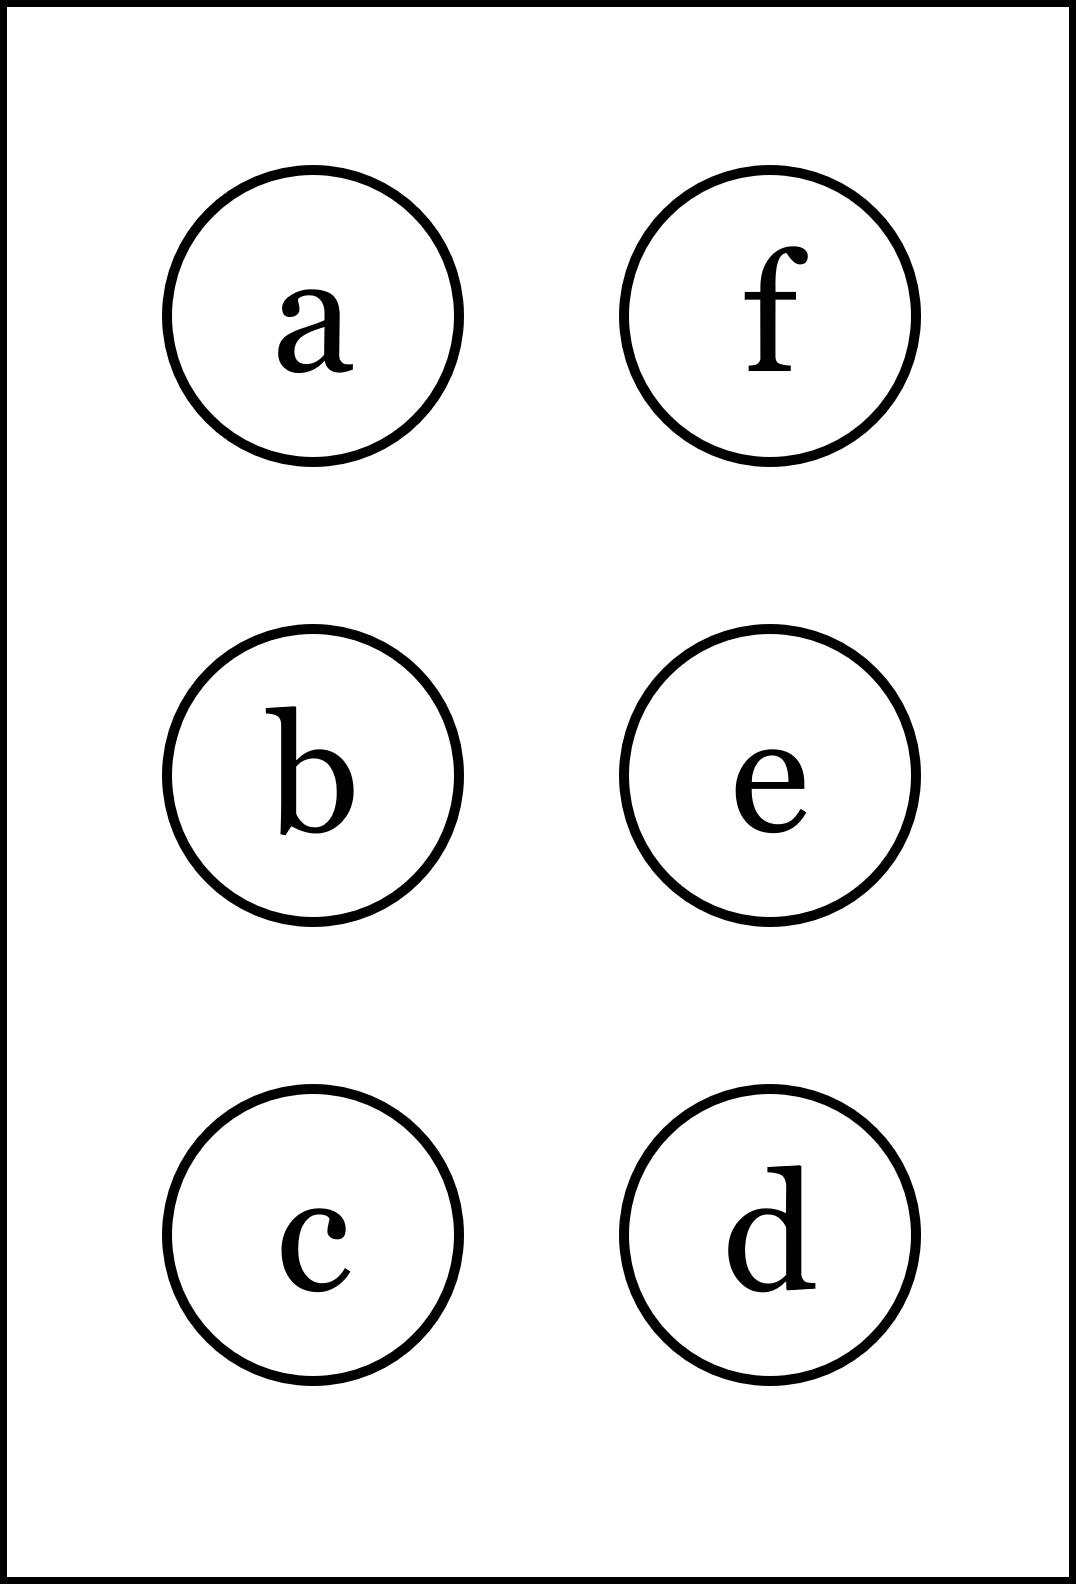
\includegraphics[height=40mm]{../images/braille.png}
{\small Písmeno Braillovej abecedy}
\end{center}
\end{minipage}
\end{center}
\end{minipage}
&
\begin{minipage}[c][99mm][t]{0.49\linewidth}
\begin{center}
\vspace{7mm}
{\huge Kubická rovnice, skupina \textit{Alpha $\alpha$} -\romannumeral4}\\[4.5mm]
\textit{Meno:}\phantom{xxxxxxxxxxxxxxxxxxxxxxxxxxxxxxxxxxxxxxxxxxxxxxxxxxxxxxxxxxxxxxxxx}\\[3.5mm]
\textbf{Vypočítej součet kořenů kubické rovnice.} Dvojitý kořen považuj do součtu za dva.\\Analogicky pro trojitý kořen. Pokud ti vyjde stejný výsledek jako je za otazníky, tak\\napravo obarvi příslušející kroužek načerno. \textbf{Spolu odevzdejte výsledné slovo}.\\[3mm]
\begin{minipage}{0.77\linewidth}
\begin{center}
\begin{varwidth}{\textwidth}
\begin{enumerate}
\large
\item $-x^3+4x^2-4x=0$\quad \dotfill\; ???\;\dotfill \quad 4
\item $2x^3-8x^2-2x+8=0$\quad \dotfill\; ???\;\dotfill \quad -6
\item $20x^3-70x^2+70x-20=0$\quad \dotfill\; ???\;\dotfill \quad $\nicefrac{7}{2}$
\item $-3x^3+5x^2+42x+40=0$\quad \dotfill\; ???\;\dotfill \quad $\nicefrac{17}{3}$
\item \quad \dotfill\; ???\;\dotfill \quad vybarvi
\item \quad \dotfill\; ???\;\dotfill \quad nebarvi
\end{enumerate}
\end{varwidth}
\end{center}
\end{minipage}
\begin{minipage}{0.20\linewidth}
\begin{center}
{\Huge\bfseries 4.} \\[2mm]
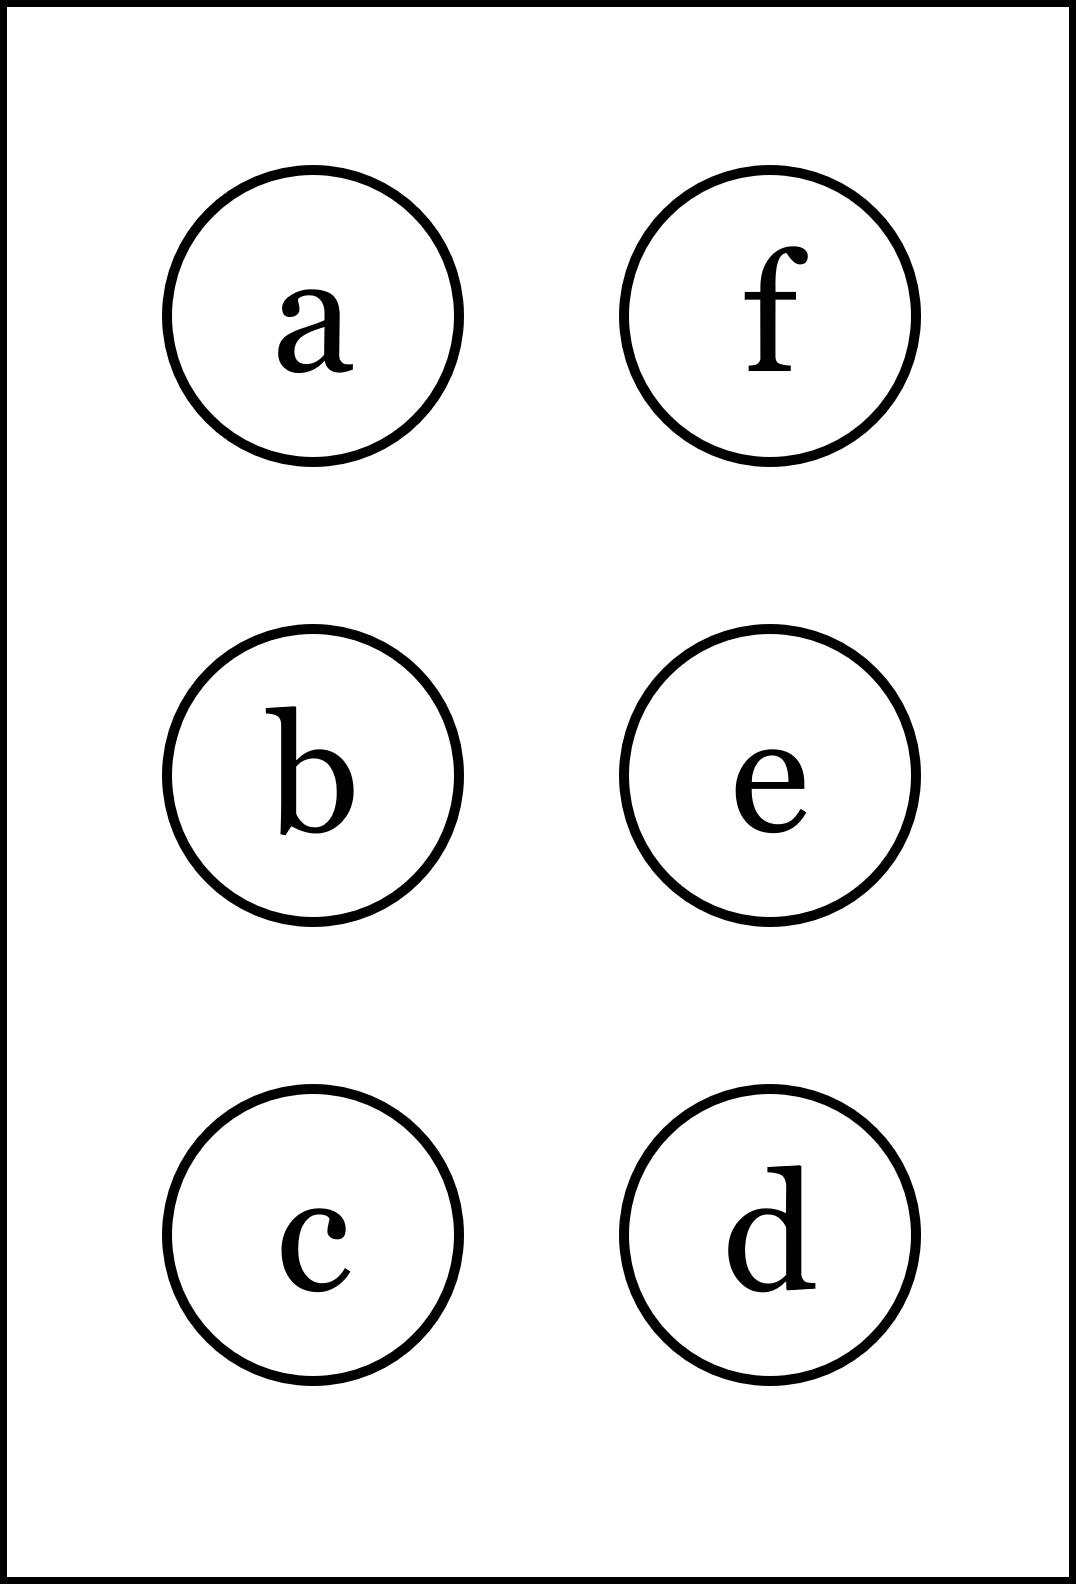
\includegraphics[height=40mm]{../images/braille.png}
{\small Písmeno Braillovej abecedy}
\end{center}
\end{minipage}
\end{center}
\end{minipage}

\end{tabular}
\begin{tikzpicture}[remember picture,overlay]\node[xshift=7mm,yshift=-100.6mm,anchor=north west] at (current page.north west){\ding{33}};\end{tikzpicture}
\begin{tikzpicture}[remember picture,overlay]\node[xshift=151.2mm,yshift=-7mm,anchor=north west,rotate=270] at (current page.north west){\ding{33}};\end{tikzpicture}
\clearpage
\thispagestyle{empty}
\begin{tabular}{c:c}
\begin{minipage}[c][99mm][t]{0.49\linewidth}
\begin{center}
\vspace{7mm}
{\huge Kubická rovnice, skupina \textit{Beta $\beta$} -\romannumeral1}\\[4.5mm]
\textit{Meno:}\phantom{xxxxxxxxxxxxxxxxxxxxxxxxxxxxxxxxxxxxxxxxxxxxxxxxxxxxxxxxxxxxxxxxx}\\[3.5mm]
\textbf{Vypočítej součet kořenů kubické rovnice.} Dvojitý kořen považuj do součtu za dva.\\Analogicky pro trojitý kořen. Pokud ti vyjde stejný výsledek jako je za otazníky, tak\\napravo obarvi příslušející kroužek načerno. \textbf{Spolu odevzdejte výsledné slovo}.\\[3mm]
\begin{minipage}{0.77\linewidth}
\begin{center}
\begin{varwidth}{\textwidth}
\begin{enumerate}
\large
\item $-2x^3+22x^2-60x=0$\quad \dotfill\; ???\;\dotfill \quad 11
\item $-3x^3-27x^2-69x-45=0$\quad \dotfill\; ???\;\dotfill \quad -9
\item $18x^3-74x+56=0$\quad \dotfill\; ???\;\dotfill \quad 0
\item $-36x^3+30x^2+36x-30=0$\quad \dotfill\; ???\;\dotfill \quad $\nicefrac{5}{6}$
\item \quad \dotfill\; ???\;\dotfill \quad vybarvi
\item \quad \dotfill\; ???\;\dotfill \quad nebarvi
\end{enumerate}
\end{varwidth}
\end{center}
\end{minipage}
\begin{minipage}{0.20\linewidth}
\begin{center}
{\Huge\bfseries 1.} \\[2mm]
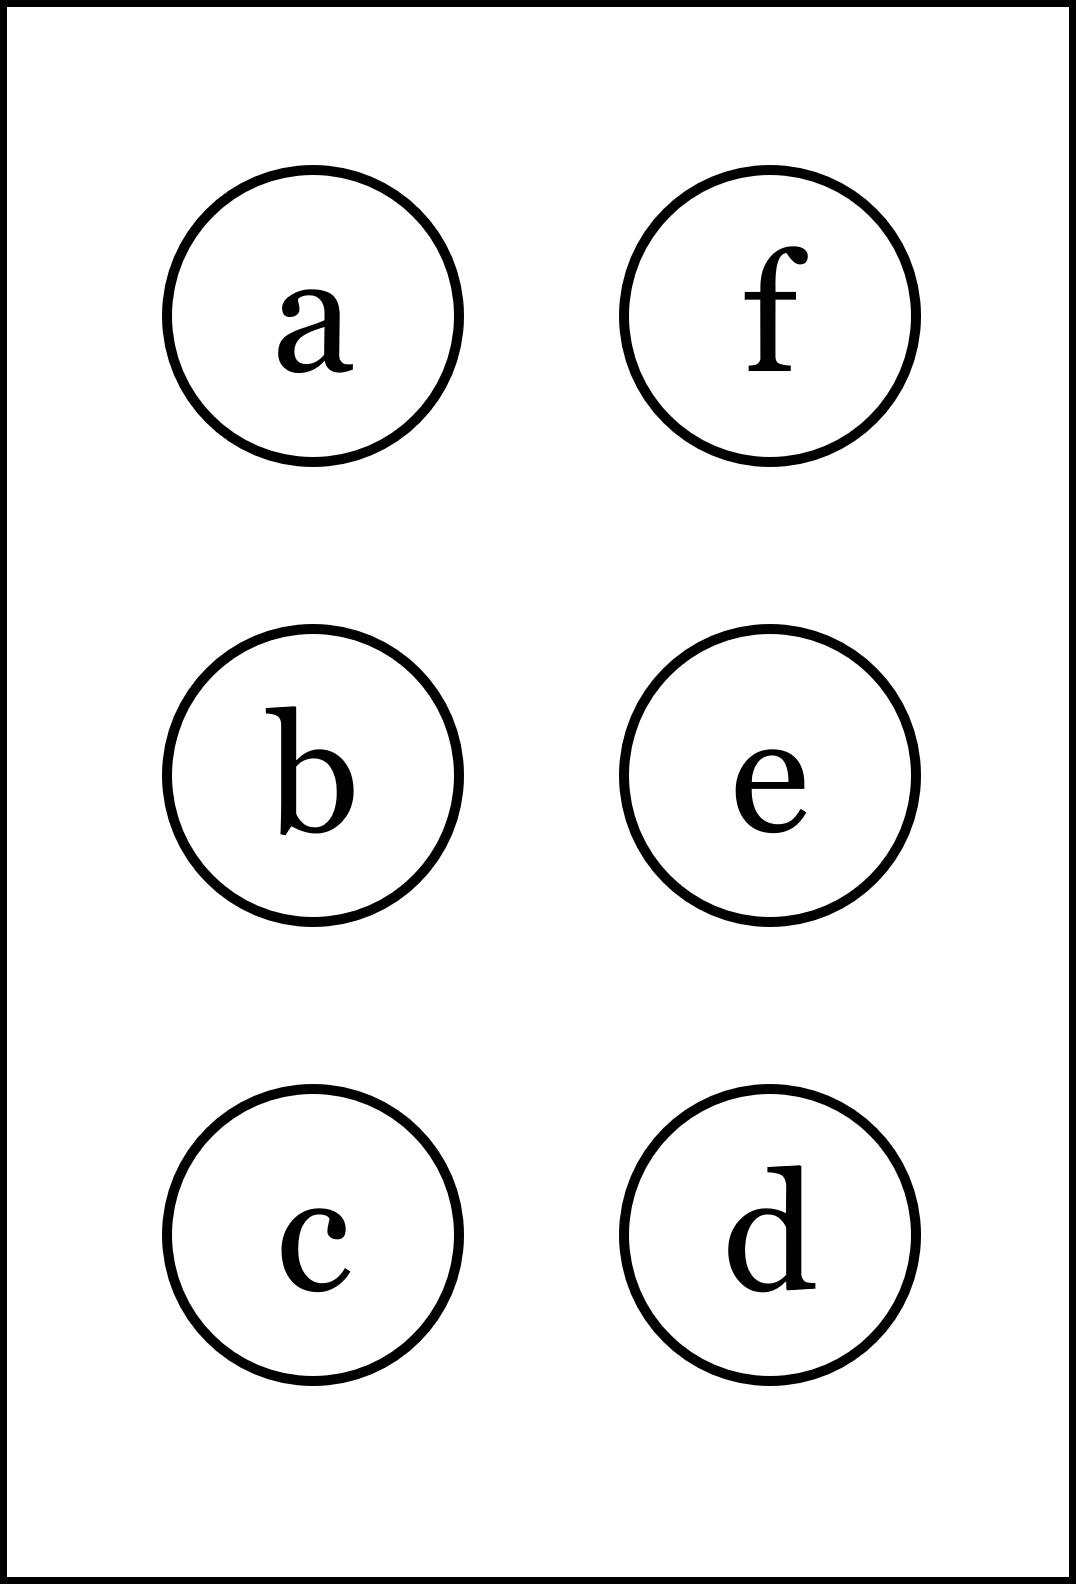
\includegraphics[height=40mm]{../images/braille.png}
{\small Písmeno Braillovej abecedy}
\end{center}
\end{minipage}
\end{center}
\end{minipage}
&
\begin{minipage}[c][99mm][t]{0.49\linewidth}
\begin{center}
\vspace{7mm}
{\huge Kubická rovnice, skupina \textit{Beta $\beta$} -\romannumeral2}\\[4.5mm]
\textit{Meno:}\phantom{xxxxxxxxxxxxxxxxxxxxxxxxxxxxxxxxxxxxxxxxxxxxxxxxxxxxxxxxxxxxxxxxx}\\[3.5mm]
\textbf{Vypočítej součet kořenů kubické rovnice.} Dvojitý kořen považuj do součtu za dva.\\Analogicky pro trojitý kořen. Pokud ti vyjde stejný výsledek jako je za otazníky, tak\\napravo obarvi příslušející kroužek načerno. \textbf{Spolu odevzdejte výsledné slovo}.\\[3mm]
\begin{minipage}{0.77\linewidth}
\begin{center}
\begin{varwidth}{\textwidth}
\begin{enumerate}
\large
\item $2x^3-20x^2+18x=0$\quad \dotfill\; ???\;\dotfill \quad 10
\item $-x^3-7x^2-7x+15=0$\quad \dotfill\; ???\;\dotfill \quad -1
\item $60x^3+20x^2-60x-20=0$\quad \dotfill\; ???\;\dotfill \quad $\nicefrac{-1}{3}$
\item $-24x^3+x^2+19x-6=0$\quad \dotfill\; ???\;\dotfill \quad $\nicefrac{31}{24}$
\item \quad \dotfill\; ???\;\dotfill \quad vybarvi
\item \quad \dotfill\; ???\;\dotfill \quad nebarvi
\end{enumerate}
\end{varwidth}
\end{center}
\end{minipage}
\begin{minipage}{0.20\linewidth}
\begin{center}
{\Huge\bfseries 2.} \\[2mm]
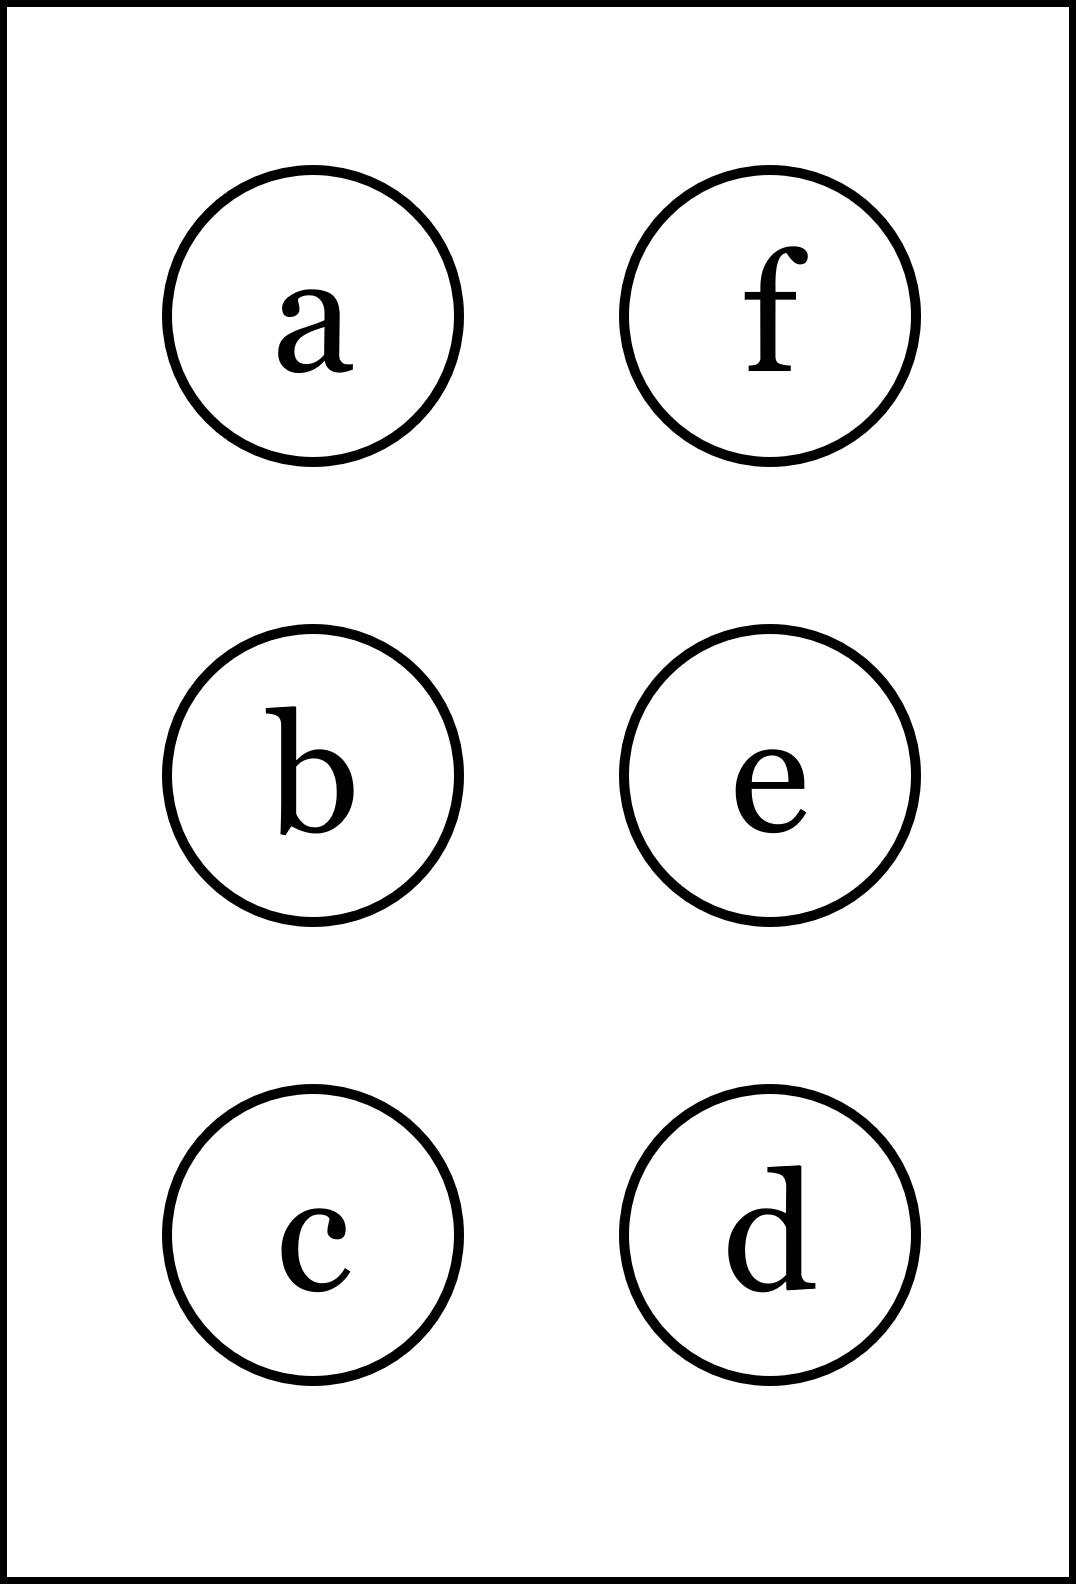
\includegraphics[height=40mm]{../images/braille.png}
{\small Písmeno Braillovej abecedy}
\end{center}
\end{minipage}
\end{center}
\end{minipage}
\\ \hdashline
\begin{minipage}[c][99mm][t]{0.49\linewidth}
\begin{center}
\vspace{7mm}
{\huge Kubická rovnice, skupina \textit{Beta $\beta$} -\romannumeral3}\\[4.5mm]
\textit{Meno:}\phantom{xxxxxxxxxxxxxxxxxxxxxxxxxxxxxxxxxxxxxxxxxxxxxxxxxxxxxxxxxxxxxxxxx}\\[3.5mm]
\textbf{Vypočítej součet kořenů kubické rovnice.} Dvojitý kořen považuj do součtu za dva.\\Analogicky pro trojitý kořen. Pokud ti vyjde stejný výsledek jako je za otazníky, tak\\napravo obarvi příslušející kroužek načerno. \textbf{Spolu odevzdejte výsledné slovo}.\\[3mm]
\begin{minipage}{0.77\linewidth}
\begin{center}
\begin{varwidth}{\textwidth}
\begin{enumerate}
\large
\item $x^3-7x^2+6x=0$\quad \dotfill\; ???\;\dotfill \quad 7
\item $x^3+7x^2+14x+8=0$\quad \dotfill\; ???\;\dotfill \quad 1
\item $-6x^3-3x^2+21x+18=0$\quad \dotfill\; ???\;\dotfill \quad $\nicefrac{-1}{2}$
\item $-9x^3-49x^2+34x+24=0$\quad \dotfill\; ???\;\dotfill \quad $\nicefrac{-59}{9}$
\item \quad \dotfill\; ???\;\dotfill \quad nebarvi
\item \quad \dotfill\; ???\;\dotfill \quad nebarvi
\end{enumerate}
\end{varwidth}
\end{center}
\end{minipage}
\begin{minipage}{0.20\linewidth}
\begin{center}
{\Huge\bfseries 3.} \\[2mm]
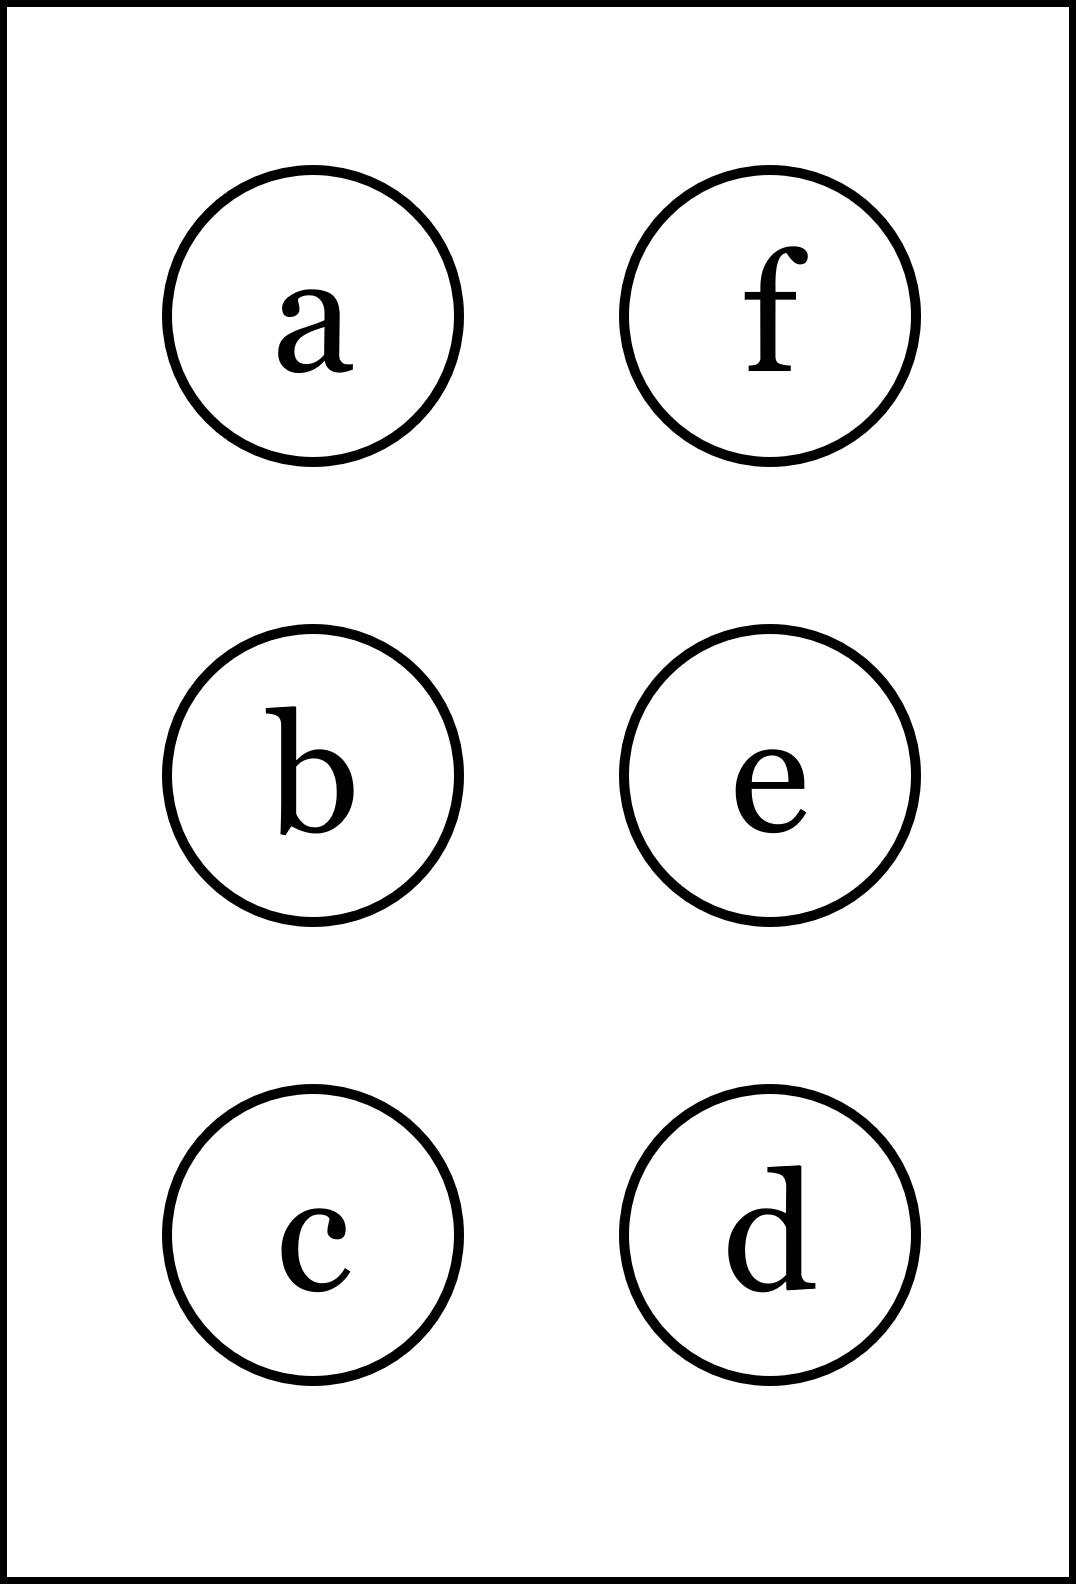
\includegraphics[height=40mm]{../images/braille.png}
{\small Písmeno Braillovej abecedy}
\end{center}
\end{minipage}
\end{center}
\end{minipage}
&
\begin{minipage}[c][99mm][t]{0.49\linewidth}
\begin{center}
\vspace{7mm}
{\huge Kubická rovnice, skupina \textit{Beta $\beta$} -\romannumeral4}\\[4.5mm]
\textit{Meno:}\phantom{xxxxxxxxxxxxxxxxxxxxxxxxxxxxxxxxxxxxxxxxxxxxxxxxxxxxxxxxxxxxxxxxx}\\[3.5mm]
\textbf{Vypočítej součet kořenů kubické rovnice.} Dvojitý kořen považuj do součtu za dva.\\Analogicky pro trojitý kořen. Pokud ti vyjde stejný výsledek jako je za otazníky, tak\\napravo obarvi příslušející kroužek načerno. \textbf{Spolu odevzdejte výsledné slovo}.\\[3mm]
\begin{minipage}{0.77\linewidth}
\begin{center}
\begin{varwidth}{\textwidth}
\begin{enumerate}
\large
\item $-x^3-4x^2+12x=0$\quad \dotfill\; ???\;\dotfill \quad -4
\item $-x^3+3x^2-3x+1=0$\quad \dotfill\; ???\;\dotfill \quad -1
\item $12x^3+18x^2-6=0$\quad \dotfill\; ???\;\dotfill \quad $\nicefrac{-5}{2}$
\item $-15x^3+22x^2+28x-24=0$\quad \dotfill\; ???\;\dotfill \quad $\nicefrac{-58}{15}$
\item \quad \dotfill\; ???\;\dotfill \quad nebarvi
\item \quad \dotfill\; ???\;\dotfill \quad nebarvi
\end{enumerate}
\end{varwidth}
\end{center}
\end{minipage}
\begin{minipage}{0.20\linewidth}
\begin{center}
{\Huge\bfseries 4.} \\[2mm]
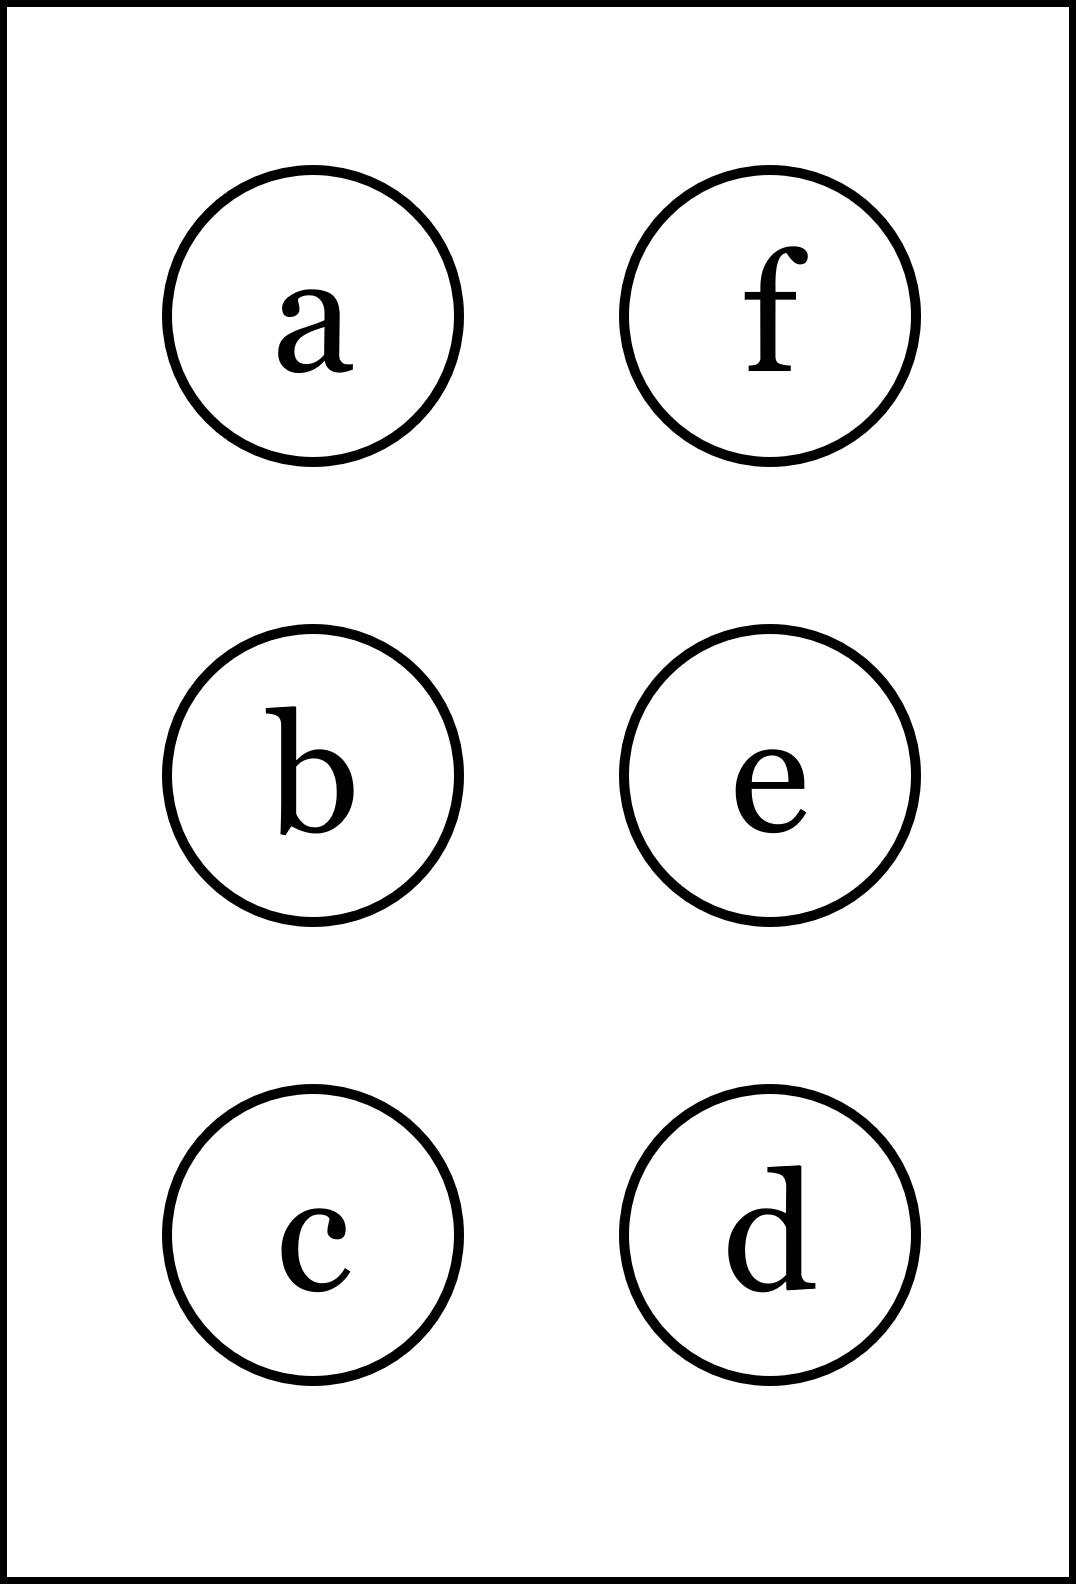
\includegraphics[height=40mm]{../images/braille.png}
{\small Písmeno Braillovej abecedy}
\end{center}
\end{minipage}
\end{center}
\end{minipage}

\end{tabular}
\begin{tikzpicture}[remember picture,overlay]\node[xshift=7mm,yshift=-100.6mm,anchor=north west] at (current page.north west){\ding{33}};\end{tikzpicture}
\begin{tikzpicture}[remember picture,overlay]\node[xshift=151.2mm,yshift=-7mm,anchor=north west,rotate=270] at (current page.north west){\ding{33}};\end{tikzpicture}
\clearpage
\thispagestyle{empty}
\begin{tabular}{c:c}
\begin{minipage}[c][99mm][t]{0.49\linewidth}
\begin{center}
\vspace{7mm}
{\huge Kubická rovnice, skupina \textit{Gamma $\gamma$} -\romannumeral1}\\[4.5mm]
\textit{Meno:}\phantom{xxxxxxxxxxxxxxxxxxxxxxxxxxxxxxxxxxxxxxxxxxxxxxxxxxxxxxxxxxxxxxxxx}\\[3.5mm]
\textbf{Vypočítej součet kořenů kubické rovnice.} Dvojitý kořen považuj do součtu za dva.\\Analogicky pro trojitý kořen. Pokud ti vyjde stejný výsledek jako je za otazníky, tak\\napravo obarvi příslušející kroužek načerno. \textbf{Spolu odevzdejte výsledné slovo}.\\[3mm]
\begin{minipage}{0.77\linewidth}
\begin{center}
\begin{varwidth}{\textwidth}
\begin{enumerate}
\large
\item $-2x^3+2x^2+24x=0$\quad \dotfill\; ???\;\dotfill \quad 1
\item $x^3+16x^2+69x+54=0$\quad \dotfill\; ???\;\dotfill \quad -4
\item $18x^3+42x^2+30x+6=0$\quad \dotfill\; ???\;\dotfill \quad $\nicefrac{5}{3}$
\item $x^3-4x^2-11x+30=0$\quad \dotfill\; ???\;\dotfill \quad 0
\item \quad \dotfill\; ???\;\dotfill \quad vybarvi
\item \quad \dotfill\; ???\;\dotfill \quad nebarvi
\end{enumerate}
\end{varwidth}
\end{center}
\end{minipage}
\begin{minipage}{0.20\linewidth}
\begin{center}
{\Huge\bfseries 1.} \\[2mm]
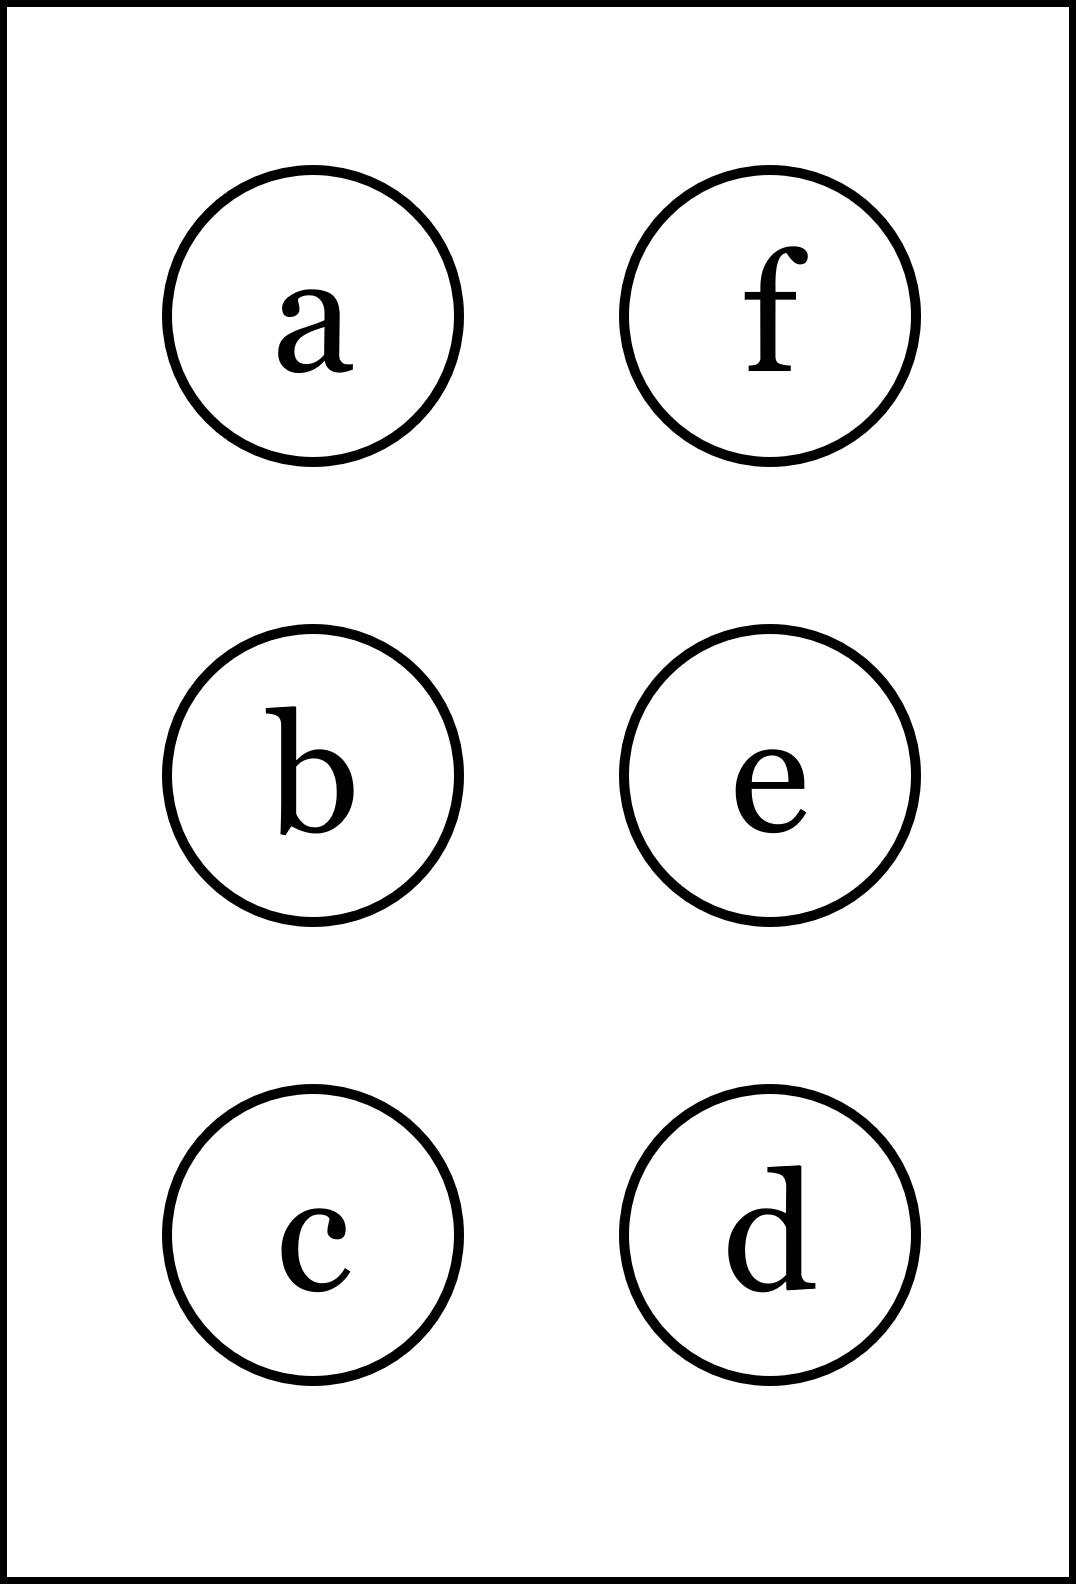
\includegraphics[height=40mm]{../images/braille.png}
{\small Písmeno Braillovej abecedy}
\end{center}
\end{minipage}
\end{center}
\end{minipage}
&
\begin{minipage}[c][99mm][t]{0.49\linewidth}
\begin{center}
\vspace{7mm}
{\huge Kubická rovnice, skupina \textit{Gamma $\gamma$} -\romannumeral2}\\[4.5mm]
\textit{Meno:}\phantom{xxxxxxxxxxxxxxxxxxxxxxxxxxxxxxxxxxxxxxxxxxxxxxxxxxxxxxxxxxxxxxxxx}\\[3.5mm]
\textbf{Vypočítej součet kořenů kubické rovnice.} Dvojitý kořen považuj do součtu za dva.\\Analogicky pro trojitý kořen. Pokud ti vyjde stejný výsledek jako je za otazníky, tak\\napravo obarvi příslušející kroužek načerno. \textbf{Spolu odevzdejte výsledné slovo}.\\[3mm]
\begin{minipage}{0.77\linewidth}
\begin{center}
\begin{varwidth}{\textwidth}
\begin{enumerate}
\large
\item $2x^3-2x^2-4x=0$\quad \dotfill\; ???\;\dotfill \quad 1
\item $-x^3-x^2+5x-3=0$\quad \dotfill\; ???\;\dotfill \quad -1
\item $24x^3-48x^2-24x+48=0$\quad \dotfill\; ???\;\dotfill \quad 2
\item $-16x^3+64x^2-51x+9=0$\quad \dotfill\; ???\;\dotfill \quad $\nicefrac{5}{2}$
\item \quad \dotfill\; ???\;\dotfill \quad nebarvi
\item \quad \dotfill\; ???\;\dotfill \quad vybarvi
\end{enumerate}
\end{varwidth}
\end{center}
\end{minipage}
\begin{minipage}{0.20\linewidth}
\begin{center}
{\Huge\bfseries 2.} \\[2mm]
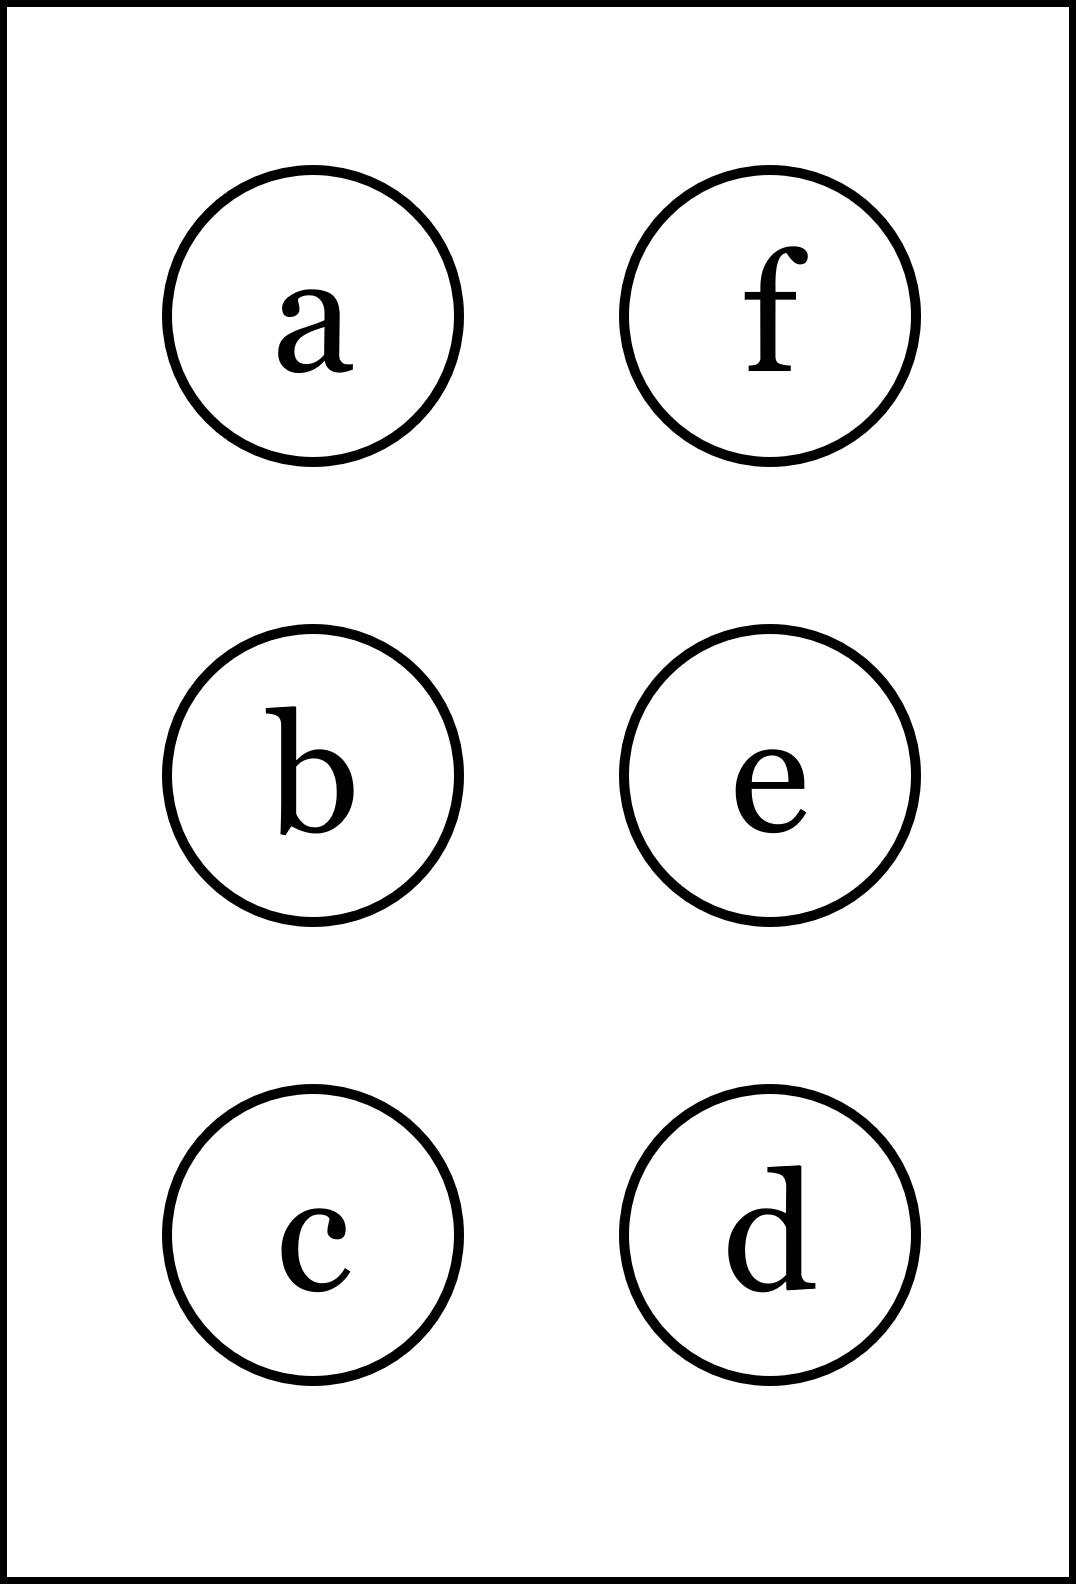
\includegraphics[height=40mm]{../images/braille.png}
{\small Písmeno Braillovej abecedy}
\end{center}
\end{minipage}
\end{center}
\end{minipage}
\\ \hdashline
\begin{minipage}[c][99mm][t]{0.49\linewidth}
\begin{center}
\vspace{7mm}
{\huge Kubická rovnice, skupina \textit{Gamma $\gamma$} -\romannumeral3}\\[4.5mm]
\textit{Meno:}\phantom{xxxxxxxxxxxxxxxxxxxxxxxxxxxxxxxxxxxxxxxxxxxxxxxxxxxxxxxxxxxxxxxxx}\\[3.5mm]
\textbf{Vypočítej součet kořenů kubické rovnice.} Dvojitý kořen považuj do součtu za dva.\\Analogicky pro trojitý kořen. Pokud ti vyjde stejný výsledek jako je za otazníky, tak\\napravo obarvi příslušející kroužek načerno. \textbf{Spolu odevzdejte výsledné slovo}.\\[3mm]
\begin{minipage}{0.77\linewidth}
\begin{center}
\begin{varwidth}{\textwidth}
\begin{enumerate}
\large
\item $-5x^3+20x=0$\quad \dotfill\; ???\;\dotfill \quad 0
\item $-x^3-5x^2+4x+20=0$\quad \dotfill\; ???\;\dotfill \quad 1
\item $-27x^3-72x^2-57x-12=0$\quad \dotfill\; ???\;\dotfill \quad $\nicefrac{-8}{3}$
\item $-8x^3-2x^2+11x+5=0$\quad \dotfill\; ???\;\dotfill \quad $\nicefrac{-11}{4}$
\item \quad \dotfill\; ???\;\dotfill \quad vybarvi
\item \quad \dotfill\; ???\;\dotfill \quad nebarvi
\end{enumerate}
\end{varwidth}
\end{center}
\end{minipage}
\begin{minipage}{0.20\linewidth}
\begin{center}
{\Huge\bfseries 3.} \\[2mm]
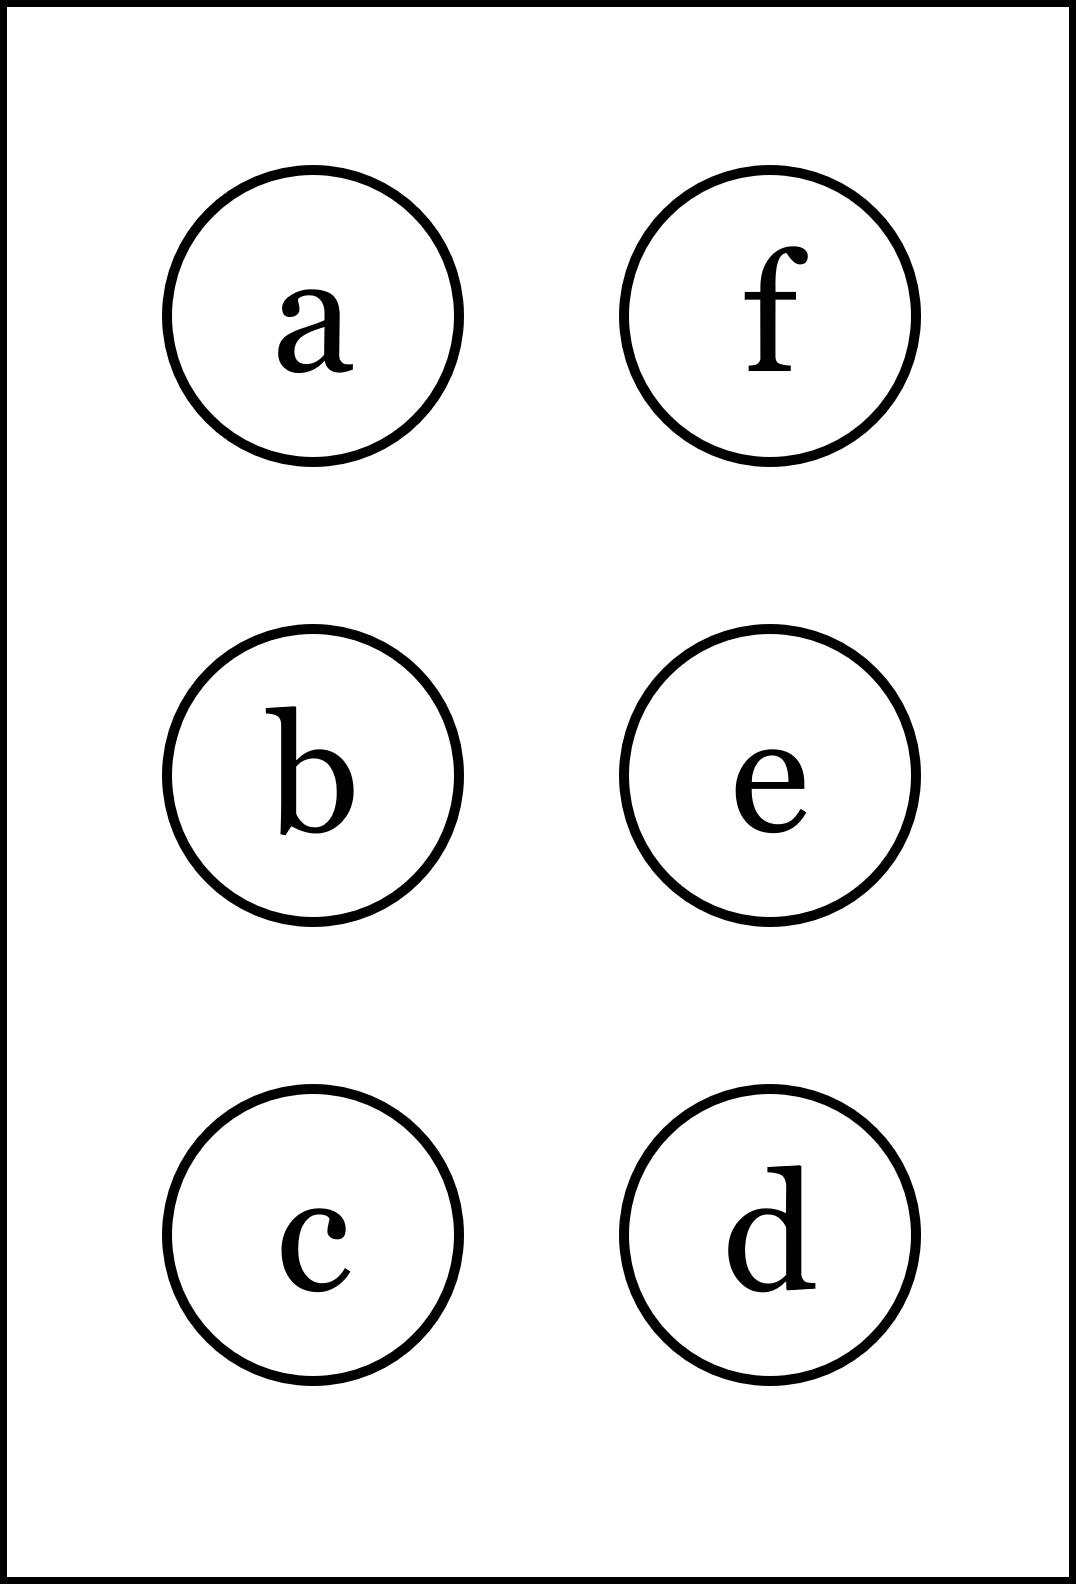
\includegraphics[height=40mm]{../images/braille.png}
{\small Písmeno Braillovej abecedy}
\end{center}
\end{minipage}
\end{center}
\end{minipage}
&
\begin{minipage}[c][99mm][t]{0.49\linewidth}
\begin{center}
\vspace{7mm}
{\huge Kubická rovnice, skupina \textit{Gamma $\gamma$} -\romannumeral4}\\[4.5mm]
\textit{Meno:}\phantom{xxxxxxxxxxxxxxxxxxxxxxxxxxxxxxxxxxxxxxxxxxxxxxxxxxxxxxxxxxxxxxxxx}\\[3.5mm]
\textbf{Vypočítej součet kořenů kubické rovnice.} Dvojitý kořen považuj do součtu za dva.\\Analogicky pro trojitý kořen. Pokud ti vyjde stejný výsledek jako je za otazníky, tak\\napravo obarvi příslušející kroužek načerno. \textbf{Spolu odevzdejte výsledné slovo}.\\[3mm]
\begin{minipage}{0.77\linewidth}
\begin{center}
\begin{varwidth}{\textwidth}
\begin{enumerate}
\large
\item $-3x^3-3x^2+6x=0$\quad \dotfill\; ???\;\dotfill \quad -3
\item $-2x^3-4x^2+42x-36=0$\quad \dotfill\; ???\;\dotfill \quad -2
\item $-3x^3+24x^2-51x+30=0$\quad \dotfill\; ???\;\dotfill \quad 8
\item $x^3-5x^2-x+5=0$\quad \dotfill\; ???\;\dotfill \quad -3
\item \quad \dotfill\; ???\;\dotfill \quad nebarvi
\item \quad \dotfill\; ???\;\dotfill \quad vybarvi
\end{enumerate}
\end{varwidth}
\end{center}
\end{minipage}
\begin{minipage}{0.20\linewidth}
\begin{center}
{\Huge\bfseries 4.} \\[2mm]
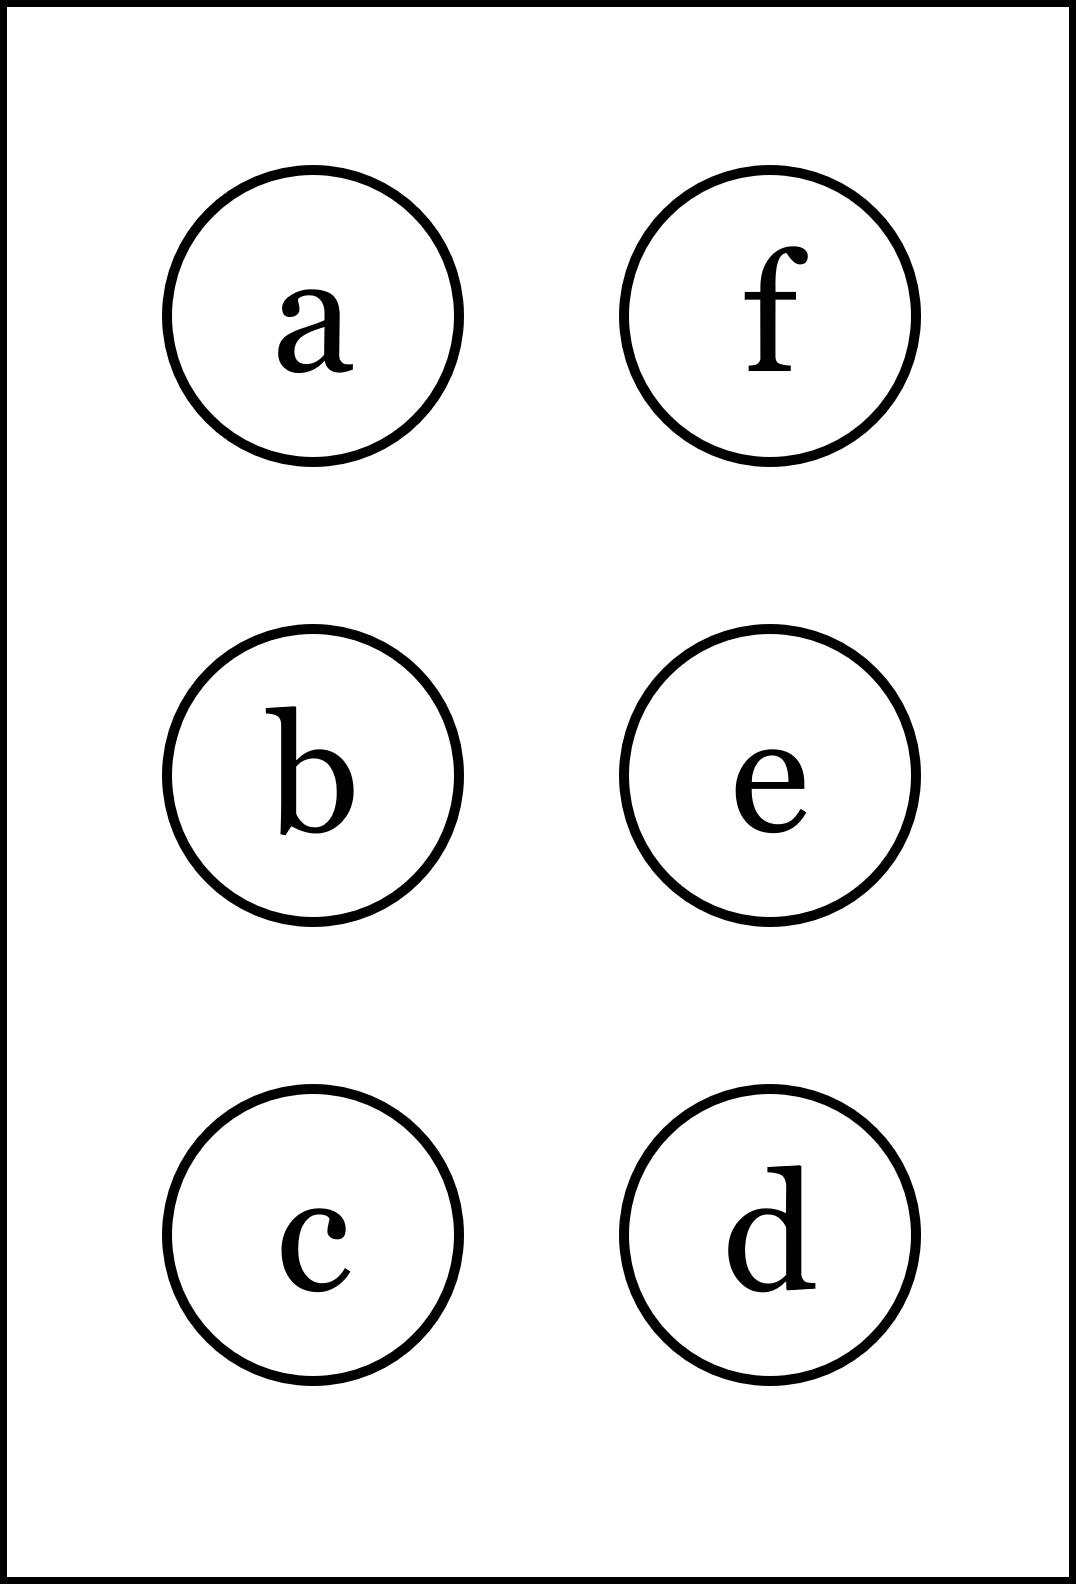
\includegraphics[height=40mm]{../images/braille.png}
{\small Písmeno Braillovej abecedy}
\end{center}
\end{minipage}
\end{center}
\end{minipage}

\end{tabular}
\begin{tikzpicture}[remember picture,overlay]\node[xshift=7mm,yshift=-100.6mm,anchor=north west] at (current page.north west){\ding{33}};\end{tikzpicture}
\begin{tikzpicture}[remember picture,overlay]\node[xshift=151.2mm,yshift=-7mm,anchor=north west,rotate=270] at (current page.north west){\ding{33}};\end{tikzpicture}
\clearpage
\thispagestyle{empty}
\begin{tabular}{c:c}
\begin{minipage}[c][99mm][t]{0.49\linewidth}
\begin{center}
\vspace{7mm}
{\huge Kubická rovnice, skupina \textit{Delta $\delta$} -\romannumeral1}\\[4.5mm]
\textit{Meno:}\phantom{xxxxxxxxxxxxxxxxxxxxxxxxxxxxxxxxxxxxxxxxxxxxxxxxxxxxxxxxxxxxxxxxx}\\[3.5mm]
\textbf{Vypočítej součet kořenů kubické rovnice.} Dvojitý kořen považuj do součtu za dva.\\Analogicky pro trojitý kořen. Pokud ti vyjde stejný výsledek jako je za otazníky, tak\\napravo obarvi příslušející kroužek načerno. \textbf{Spolu odevzdejte výsledné slovo}.\\[3mm]
\begin{minipage}{0.77\linewidth}
\begin{center}
\begin{varwidth}{\textwidth}
\begin{enumerate}
\large
\item $6x^3-12x^2+6x=0$\quad \dotfill\; ???\;\dotfill \quad 2
\item $3x^3+18x^2+27x+12=0$\quad \dotfill\; ???\;\dotfill \quad -6
\item $-2x^3-14x^2+2x+14=0$\quad \dotfill\; ???\;\dotfill \quad -7
\item $-2x^3+7x^2+14x-40=0$\quad \dotfill\; ???\;\dotfill \quad $\nicefrac{9}{2}$
\item \quad \dotfill\; ???\;\dotfill \quad vybarvi
\item \quad \dotfill\; ???\;\dotfill \quad nebarvi
\end{enumerate}
\end{varwidth}
\end{center}
\end{minipage}
\begin{minipage}{0.20\linewidth}
\begin{center}
{\Huge\bfseries 1.} \\[2mm]
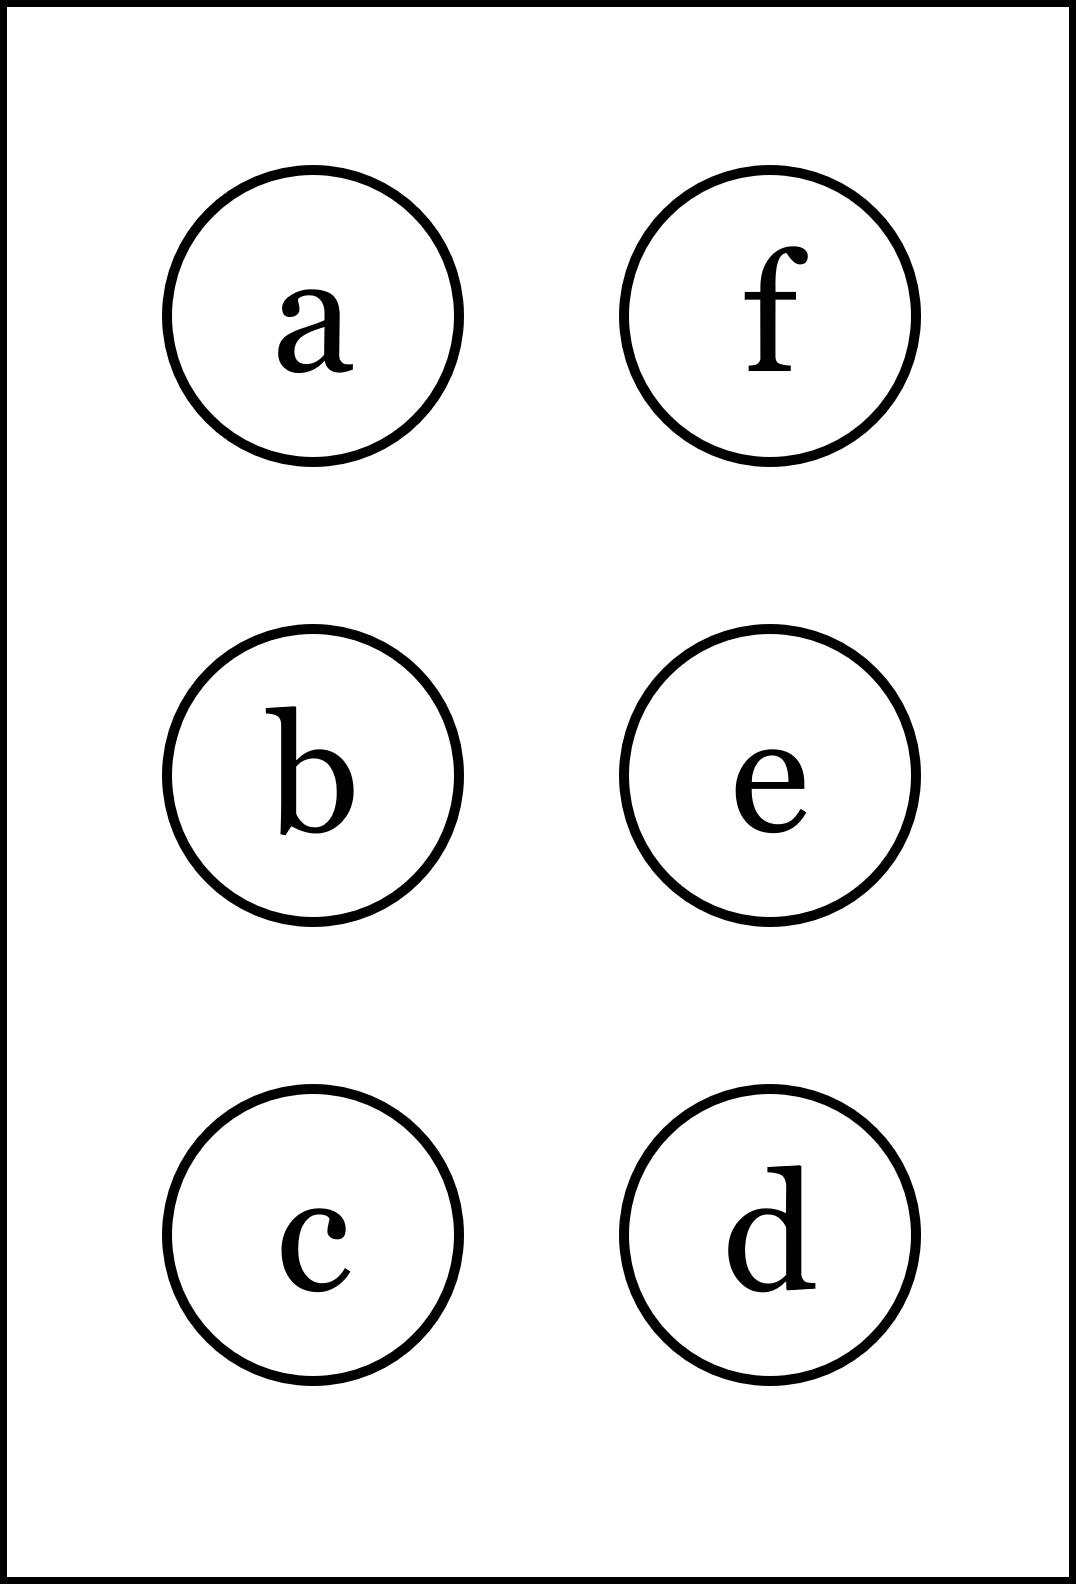
\includegraphics[height=40mm]{../images/braille.png}
{\small Písmeno Braillovej abecedy}
\end{center}
\end{minipage}
\end{center}
\end{minipage}
&
\begin{minipage}[c][99mm][t]{0.49\linewidth}
\begin{center}
\vspace{7mm}
{\huge Kubická rovnice, skupina \textit{Delta $\delta$} -\romannumeral2}\\[4.5mm]
\textit{Meno:}\phantom{xxxxxxxxxxxxxxxxxxxxxxxxxxxxxxxxxxxxxxxxxxxxxxxxxxxxxxxxxxxxxxxxx}\\[3.5mm]
\textbf{Vypočítej součet kořenů kubické rovnice.} Dvojitý kořen považuj do součtu za dva.\\Analogicky pro trojitý kořen. Pokud ti vyjde stejný výsledek jako je za otazníky, tak\\napravo obarvi příslušející kroužek načerno. \textbf{Spolu odevzdejte výsledné slovo}.\\[3mm]
\begin{minipage}{0.77\linewidth}
\begin{center}
\begin{varwidth}{\textwidth}
\begin{enumerate}
\large
\item $2x^3-12x^2+10x=0$\quad \dotfill\; ???\;\dotfill \quad 6
\item $-4x^3+24x^2-12x-40=0$\quad \dotfill\; ???\;\dotfill \quad -2
\item $48x^3+84x^2+24x-12=0$\quad \dotfill\; ???\;\dotfill \quad $\nicefrac{1}{4}$
\item $4x^3+9x^2-43x-60=0$\quad \dotfill\; ???\;\dotfill \quad $\nicefrac{-23}{4}$
\item \quad \dotfill\; ???\;\dotfill \quad nebarvi
\item \quad \dotfill\; ???\;\dotfill \quad nebarvi
\end{enumerate}
\end{varwidth}
\end{center}
\end{minipage}
\begin{minipage}{0.20\linewidth}
\begin{center}
{\Huge\bfseries 2.} \\[2mm]
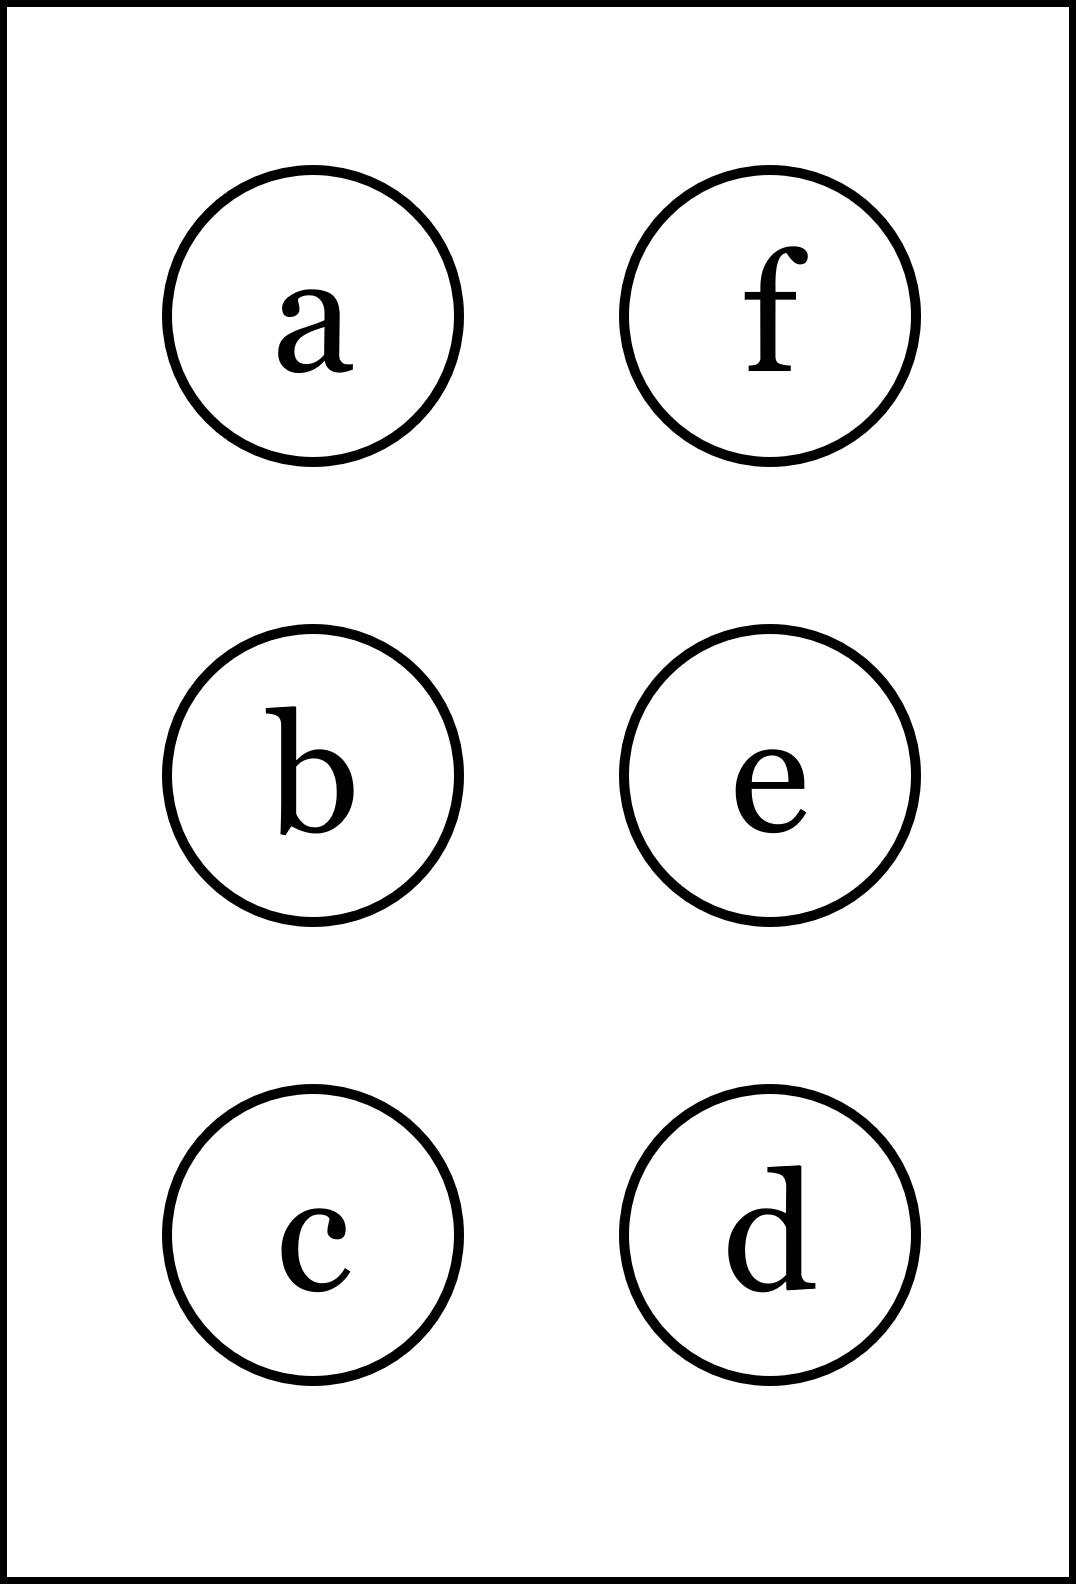
\includegraphics[height=40mm]{../images/braille.png}
{\small Písmeno Braillovej abecedy}
\end{center}
\end{minipage}
\end{center}
\end{minipage}
\\ \hdashline
\begin{minipage}[c][99mm][t]{0.49\linewidth}
\begin{center}
\vspace{7mm}
{\huge Kubická rovnice, skupina \textit{Delta $\delta$} -\romannumeral3}\\[4.5mm]
\textit{Meno:}\phantom{xxxxxxxxxxxxxxxxxxxxxxxxxxxxxxxxxxxxxxxxxxxxxxxxxxxxxxxxxxxxxxxxx}\\[3.5mm]
\textbf{Vypočítej součet kořenů kubické rovnice.} Dvojitý kořen považuj do součtu za dva.\\Analogicky pro trojitý kořen. Pokud ti vyjde stejný výsledek jako je za otazníky, tak\\napravo obarvi příslušející kroužek načerno. \textbf{Spolu odevzdejte výsledné slovo}.\\[3mm]
\begin{minipage}{0.77\linewidth}
\begin{center}
\begin{varwidth}{\textwidth}
\begin{enumerate}
\large
\item $2x^3+4x^2-6x=0$\quad \dotfill\; ???\;\dotfill \quad -4
\item $-2x^3-2x^2+8x+8=0$\quad \dotfill\; ???\;\dotfill \quad -1
\item $-48x^3-96x^2-60x-12=0$\quad \dotfill\; ???\;\dotfill \quad -2
\item $2x^3+13x^2+13x-10=0$\quad \dotfill\; ???\;\dotfill \quad $\nicefrac{15}{2}$
\item \quad \dotfill\; ???\;\dotfill \quad nebarvi
\item \quad \dotfill\; ???\;\dotfill \quad vybarvi
\end{enumerate}
\end{varwidth}
\end{center}
\end{minipage}
\begin{minipage}{0.20\linewidth}
\begin{center}
{\Huge\bfseries 3.} \\[2mm]
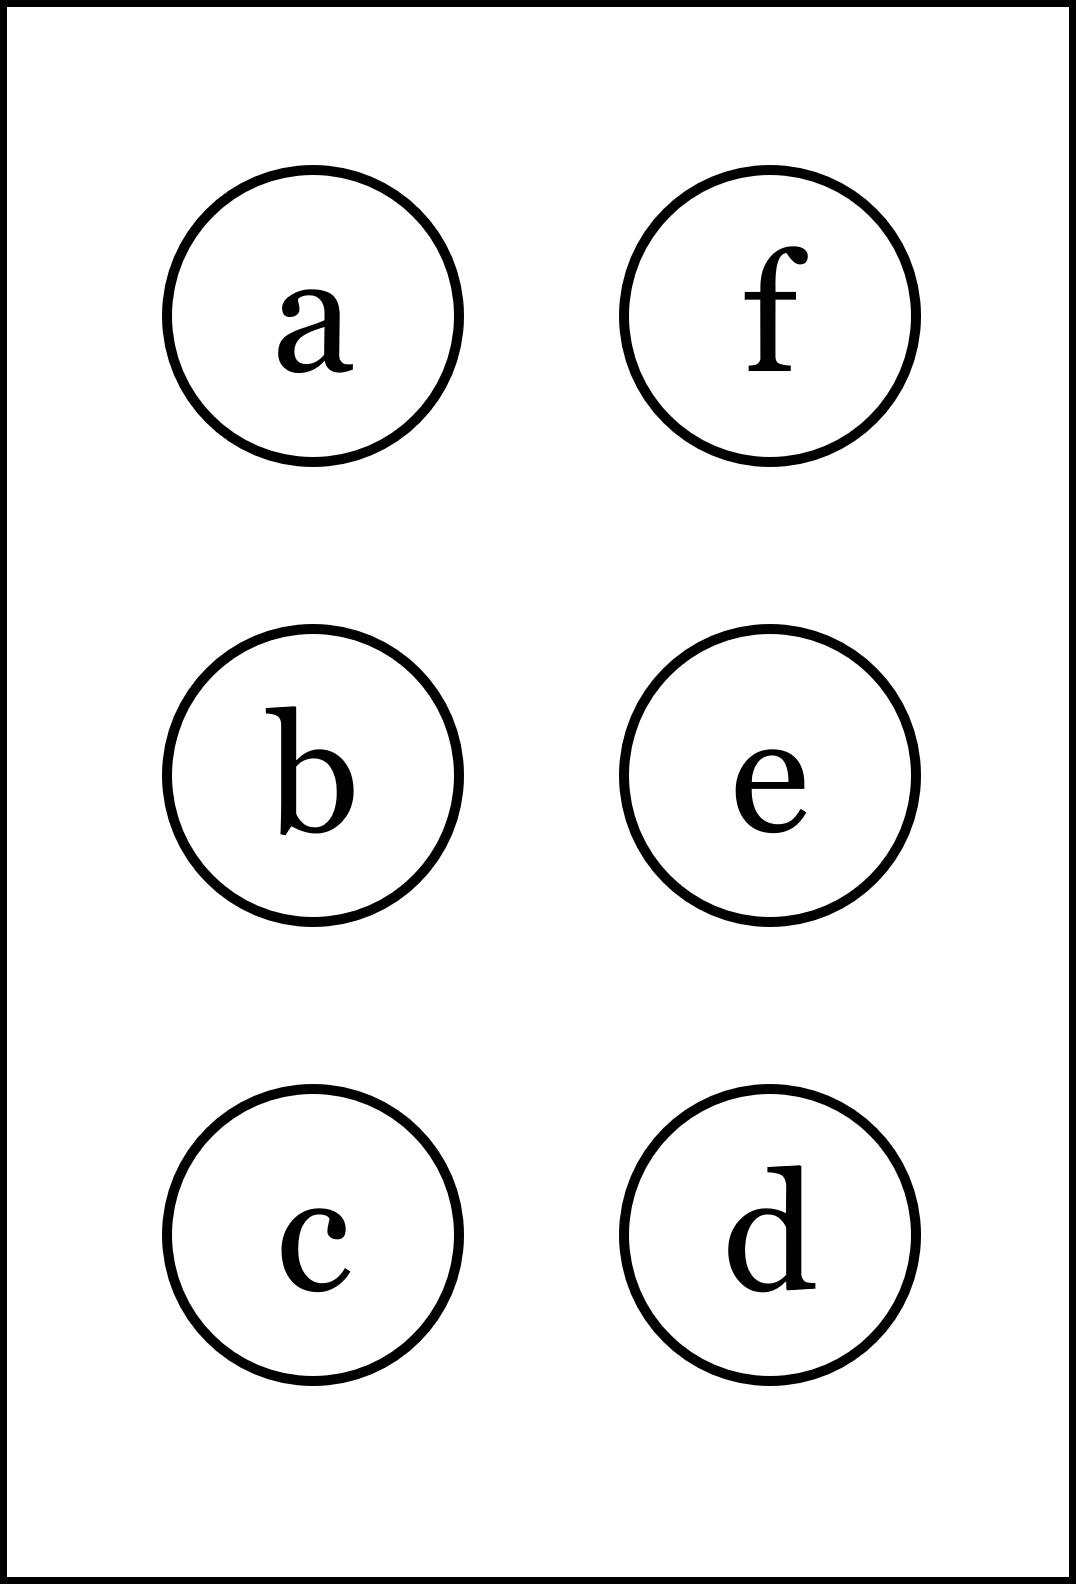
\includegraphics[height=40mm]{../images/braille.png}
{\small Písmeno Braillovej abecedy}
\end{center}
\end{minipage}
\end{center}
\end{minipage}
&
\begin{minipage}[c][99mm][t]{0.49\linewidth}
\begin{center}
\vspace{7mm}
{\huge Kubická rovnice, skupina \textit{Delta $\delta$} -\romannumeral4}\\[4.5mm]
\textit{Meno:}\phantom{xxxxxxxxxxxxxxxxxxxxxxxxxxxxxxxxxxxxxxxxxxxxxxxxxxxxxxxxxxxxxxxxx}\\[3.5mm]
\textbf{Vypočítej součet kořenů kubické rovnice.} Dvojitý kořen považuj do součtu za dva.\\Analogicky pro trojitý kořen. Pokud ti vyjde stejný výsledek jako je za otazníky, tak\\napravo obarvi příslušející kroužek načerno. \textbf{Spolu odevzdejte výsledné slovo}.\\[3mm]
\begin{minipage}{0.77\linewidth}
\begin{center}
\begin{varwidth}{\textwidth}
\begin{enumerate}
\large
\item $-6x^3-30x^2-36x=0$\quad \dotfill\; ???\;\dotfill \quad -5
\item $-2x^3-10x^2+16x+24=0$\quad \dotfill\; ???\;\dotfill \quad 7
\item $-5x^3-40x^2-85x-50=0$\quad \dotfill\; ???\;\dotfill \quad -4
\item $10x^3+3x^2-16x+3=0$\quad \dotfill\; ???\;\dotfill \quad $\nicefrac{-7}{10}$
\item \quad \dotfill\; ???\;\dotfill \quad nebarvi
\item \quad \dotfill\; ???\;\dotfill \quad nebarvi
\end{enumerate}
\end{varwidth}
\end{center}
\end{minipage}
\begin{minipage}{0.20\linewidth}
\begin{center}
{\Huge\bfseries 4.} \\[2mm]
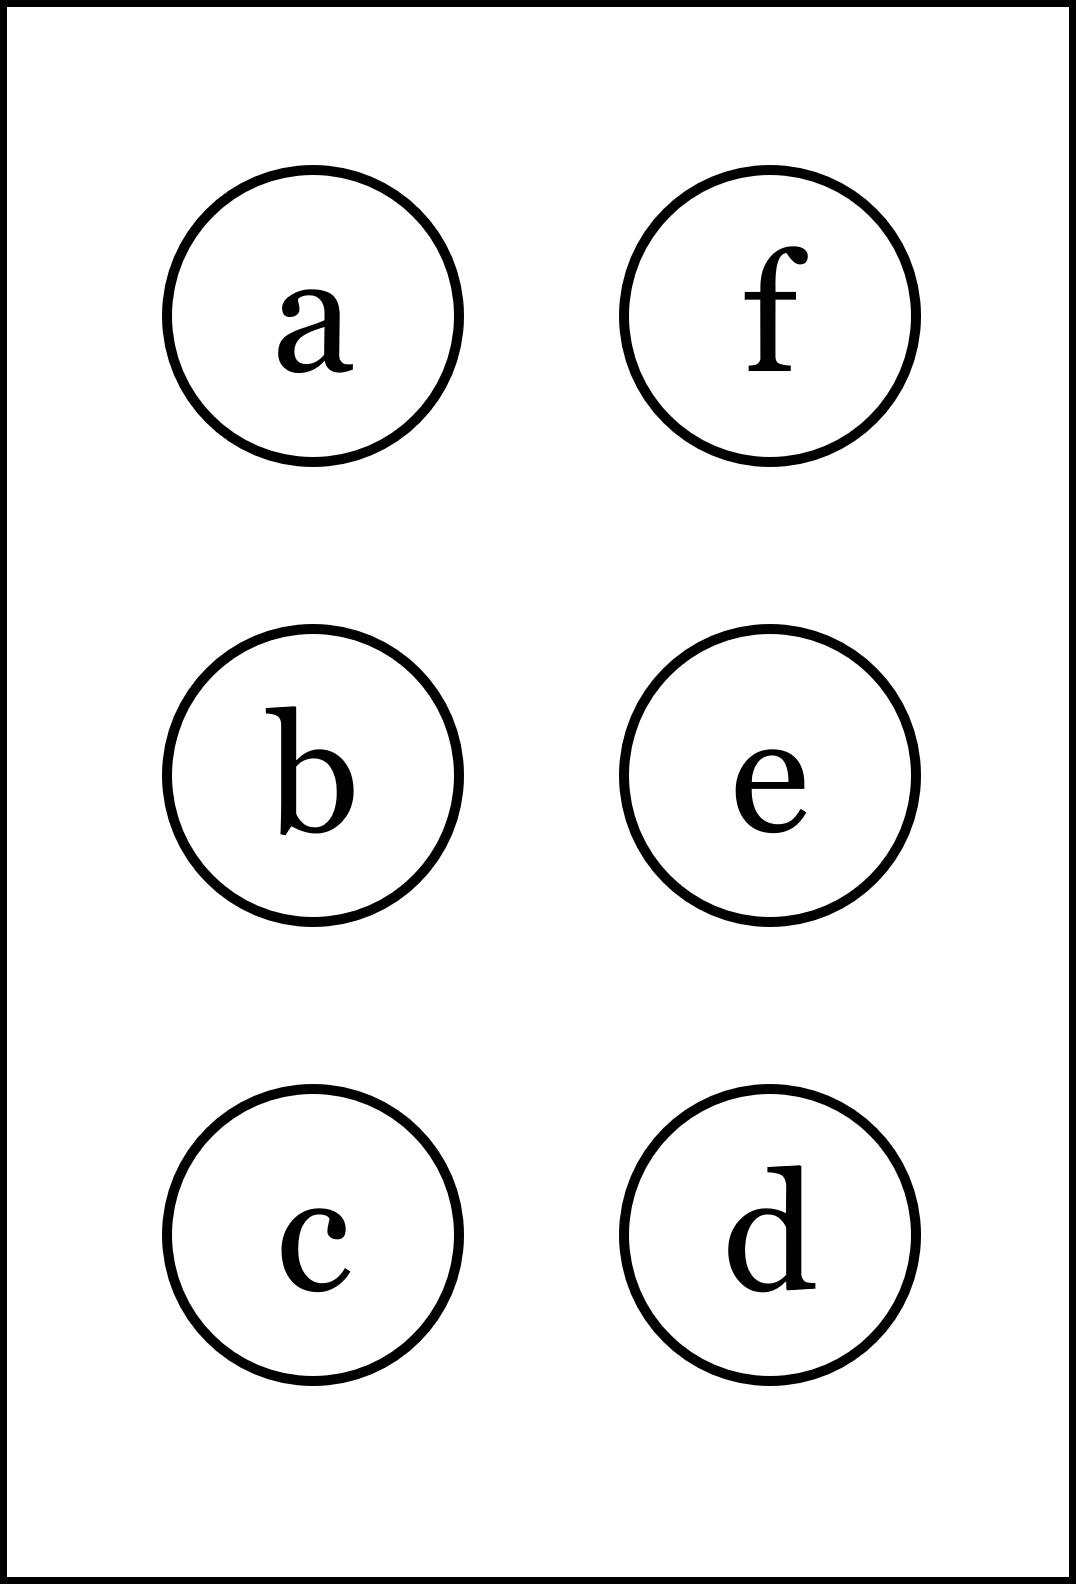
\includegraphics[height=40mm]{../images/braille.png}
{\small Písmeno Braillovej abecedy}
\end{center}
\end{minipage}
\end{center}
\end{minipage}

\end{tabular}
\begin{tikzpicture}[remember picture,overlay]\node[xshift=7mm,yshift=-100.6mm,anchor=north west] at (current page.north west){\ding{33}};\end{tikzpicture}
\begin{tikzpicture}[remember picture,overlay]\node[xshift=151.2mm,yshift=-7mm,anchor=north west,rotate=270] at (current page.north west){\ding{33}};\end{tikzpicture}
\clearpage
\thispagestyle{empty}
\begin{tabular}{c:c}
\begin{minipage}[c][99mm][t]{0.49\linewidth}
\begin{center}
\vspace{7mm}
{\huge Kubická rovnice, skupina \textit{Epsilon $\epsilon$} -\romannumeral1}\\[4.5mm]
\textit{Meno:}\phantom{xxxxxxxxxxxxxxxxxxxxxxxxxxxxxxxxxxxxxxxxxxxxxxxxxxxxxxxxxxxxxxxxx}\\[3.5mm]
\textbf{Vypočítej součet kořenů kubické rovnice.} Dvojitý kořen považuj do součtu za dva.\\Analogicky pro trojitý kořen. Pokud ti vyjde stejný výsledek jako je za otazníky, tak\\napravo obarvi příslušející kroužek načerno. \textbf{Spolu odevzdejte výsledné slovo}.\\[3mm]
\begin{minipage}{0.77\linewidth}
\begin{center}
\begin{varwidth}{\textwidth}
\begin{enumerate}
\large
\item $-2x^3-10x^2-8x=0$\quad \dotfill\; ???\;\dotfill \quad -5
\item $x^3+7x^2+4x-12=0$\quad \dotfill\; ???\;\dotfill \quad -7
\item $9x^3+17x^2-29x+3=0$\quad \dotfill\; ???\;\dotfill \quad $\nicefrac{19}{9}$
\item $-x^3-2x^2+19x+20=0$\quad \dotfill\; ???\;\dotfill \quad 8
\item \quad \dotfill\; ???\;\dotfill \quad vybarvi
\item \quad \dotfill\; ???\;\dotfill \quad nebarvi
\end{enumerate}
\end{varwidth}
\end{center}
\end{minipage}
\begin{minipage}{0.20\linewidth}
\begin{center}
{\Huge\bfseries 1.} \\[2mm]
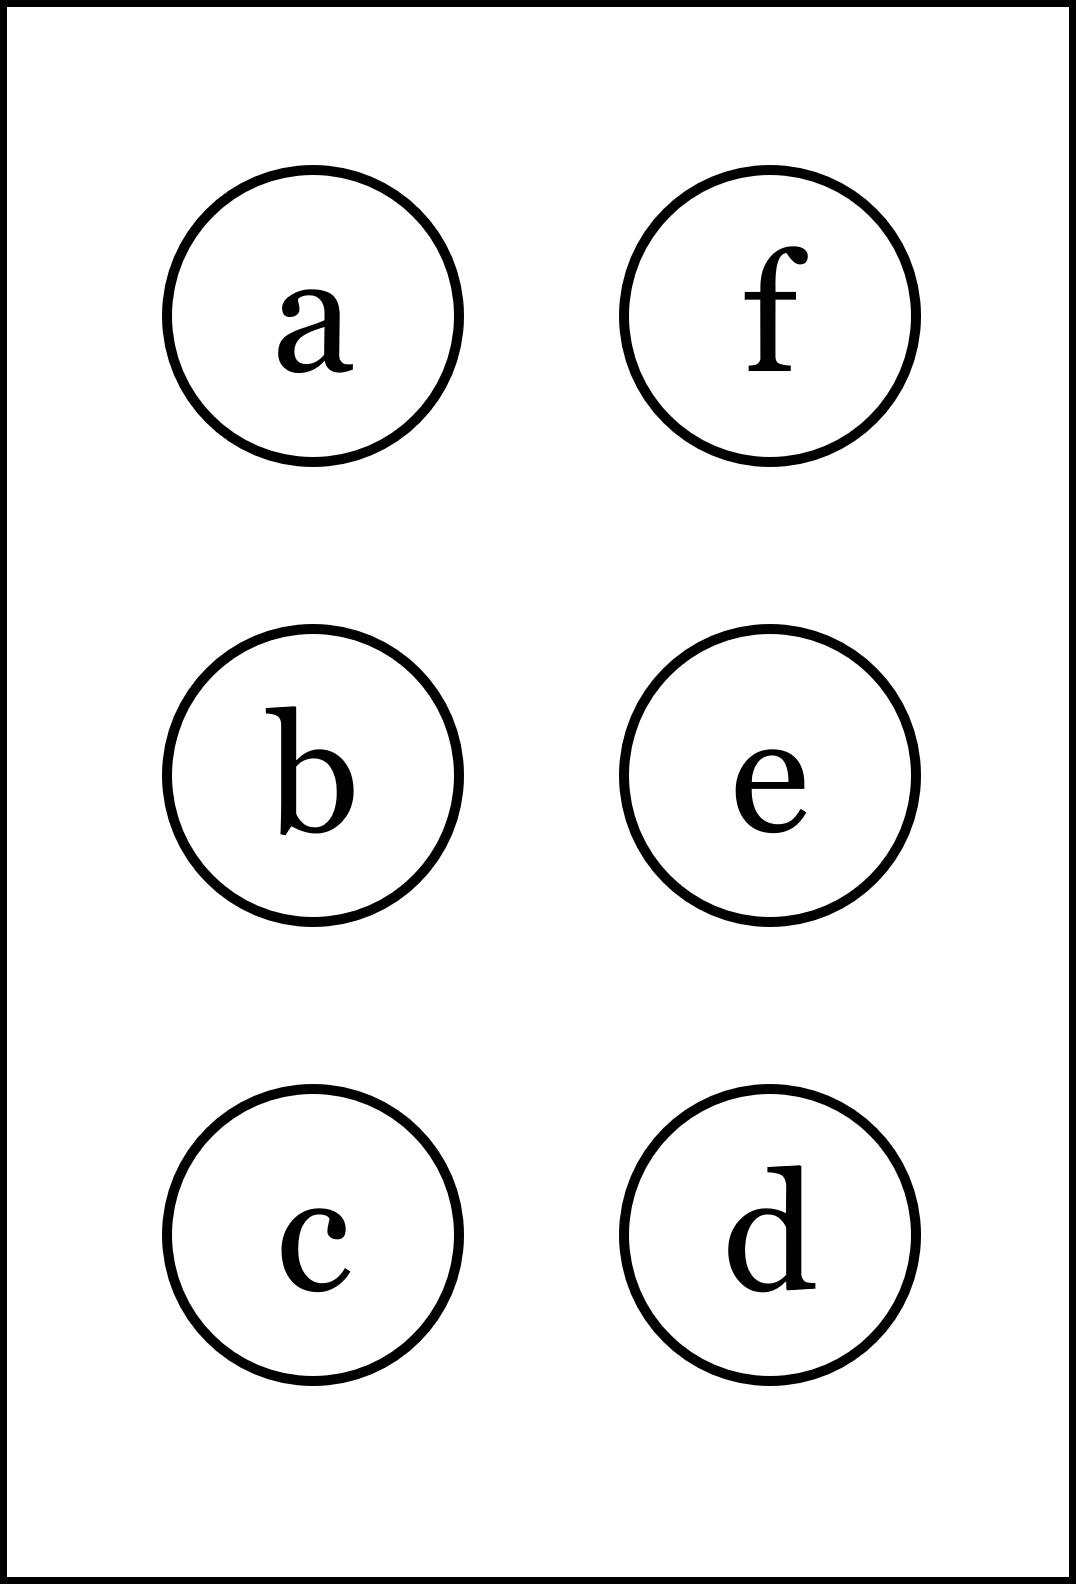
\includegraphics[height=40mm]{../images/braille.png}
{\small Písmeno Braillovej abecedy}
\end{center}
\end{minipage}
\end{center}
\end{minipage}
&
\begin{minipage}[c][99mm][t]{0.49\linewidth}
\begin{center}
\vspace{7mm}
{\huge Kubická rovnice, skupina \textit{Epsilon $\epsilon$} -\romannumeral2}\\[4.5mm]
\textit{Meno:}\phantom{xxxxxxxxxxxxxxxxxxxxxxxxxxxxxxxxxxxxxxxxxxxxxxxxxxxxxxxxxxxxxxxxx}\\[3.5mm]
\textbf{Vypočítej součet kořenů kubické rovnice.} Dvojitý kořen považuj do součtu za dva.\\Analogicky pro trojitý kořen. Pokud ti vyjde stejný výsledek jako je za otazníky, tak\\napravo obarvi příslušející kroužek načerno. \textbf{Spolu odevzdejte výsledné slovo}.\\[3mm]
\begin{minipage}{0.77\linewidth}
\begin{center}
\begin{varwidth}{\textwidth}
\begin{enumerate}
\large
\item $-2x^3+2x^2+40x=0$\quad \dotfill\; ???\;\dotfill \quad 1
\item $x^3+x^2-16x-16=0$\quad \dotfill\; ???\;\dotfill \quad 7
\item $-24x^3-16x^2+24x+16=0$\quad \dotfill\; ???\;\dotfill \quad $\nicefrac{-2}{3}$
\item $8x^3-6x+2=0$\quad \dotfill\; ???\;\dotfill \quad -1
\item \quad \dotfill\; ???\;\dotfill \quad vybarvi
\item \quad \dotfill\; ???\;\dotfill \quad nebarvi
\end{enumerate}
\end{varwidth}
\end{center}
\end{minipage}
\begin{minipage}{0.20\linewidth}
\begin{center}
{\Huge\bfseries 2.} \\[2mm]
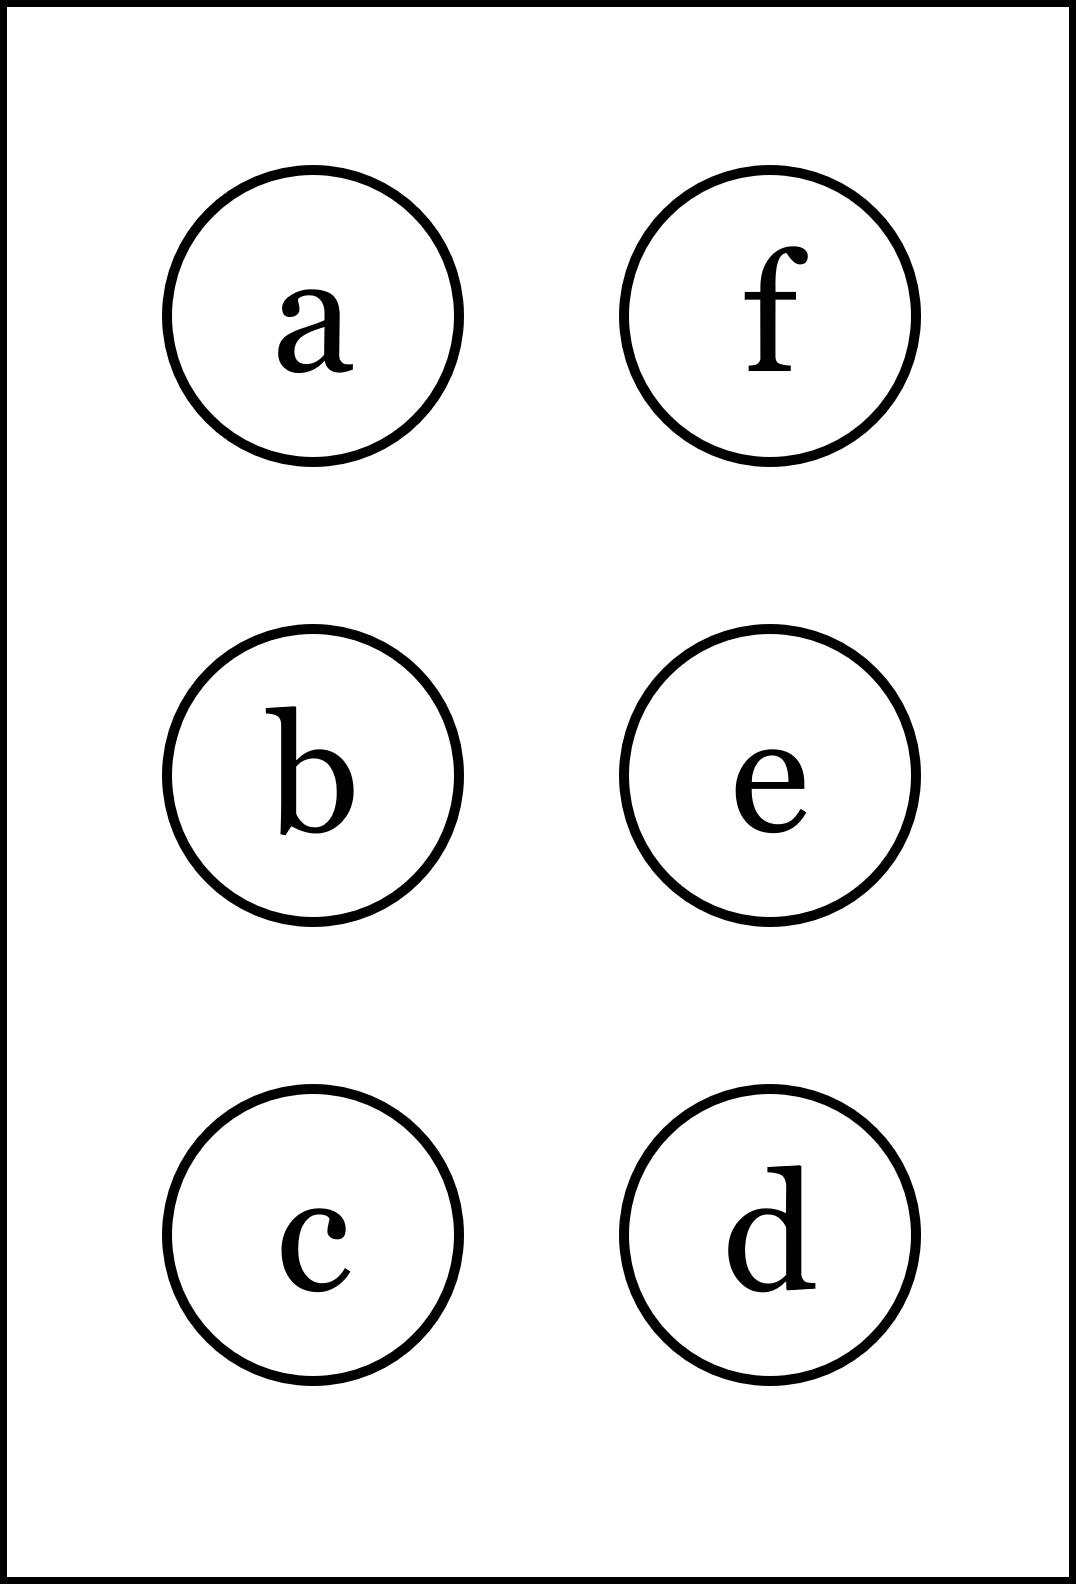
\includegraphics[height=40mm]{../images/braille.png}
{\small Písmeno Braillovej abecedy}
\end{center}
\end{minipage}
\end{center}
\end{minipage}
\\ \hdashline
\begin{minipage}[c][99mm][t]{0.49\linewidth}
\begin{center}
\vspace{7mm}
{\huge Kubická rovnice, skupina \textit{Epsilon $\epsilon$} -\romannumeral3}\\[4.5mm]
\textit{Meno:}\phantom{xxxxxxxxxxxxxxxxxxxxxxxxxxxxxxxxxxxxxxxxxxxxxxxxxxxxxxxxxxxxxxxxx}\\[3.5mm]
\textbf{Vypočítej součet kořenů kubické rovnice.} Dvojitý kořen považuj do součtu za dva.\\Analogicky pro trojitý kořen. Pokud ti vyjde stejný výsledek jako je za otazníky, tak\\napravo obarvi příslušející kroužek načerno. \textbf{Spolu odevzdejte výsledné slovo}.\\[3mm]
\begin{minipage}{0.77\linewidth}
\begin{center}
\begin{varwidth}{\textwidth}
\begin{enumerate}
\large
\item $x^3-2x^2+x=0$\quad \dotfill\; ???\;\dotfill \quad 2
\item $-x^3+3x^2+25x+21=0$\quad \dotfill\; ???\;\dotfill \quad 3
\item $3x^3+9x^2-3x-9=0$\quad \dotfill\; ???\;\dotfill \quad -3
\item $9x^3+39x^2-48=0$\quad \dotfill\; ???\;\dotfill \quad $\nicefrac{-5}{3}$
\item \quad \dotfill\; ???\;\dotfill \quad vybarvi
\item \quad \dotfill\; ???\;\dotfill \quad nebarvi
\end{enumerate}
\end{varwidth}
\end{center}
\end{minipage}
\begin{minipage}{0.20\linewidth}
\begin{center}
{\Huge\bfseries 3.} \\[2mm]
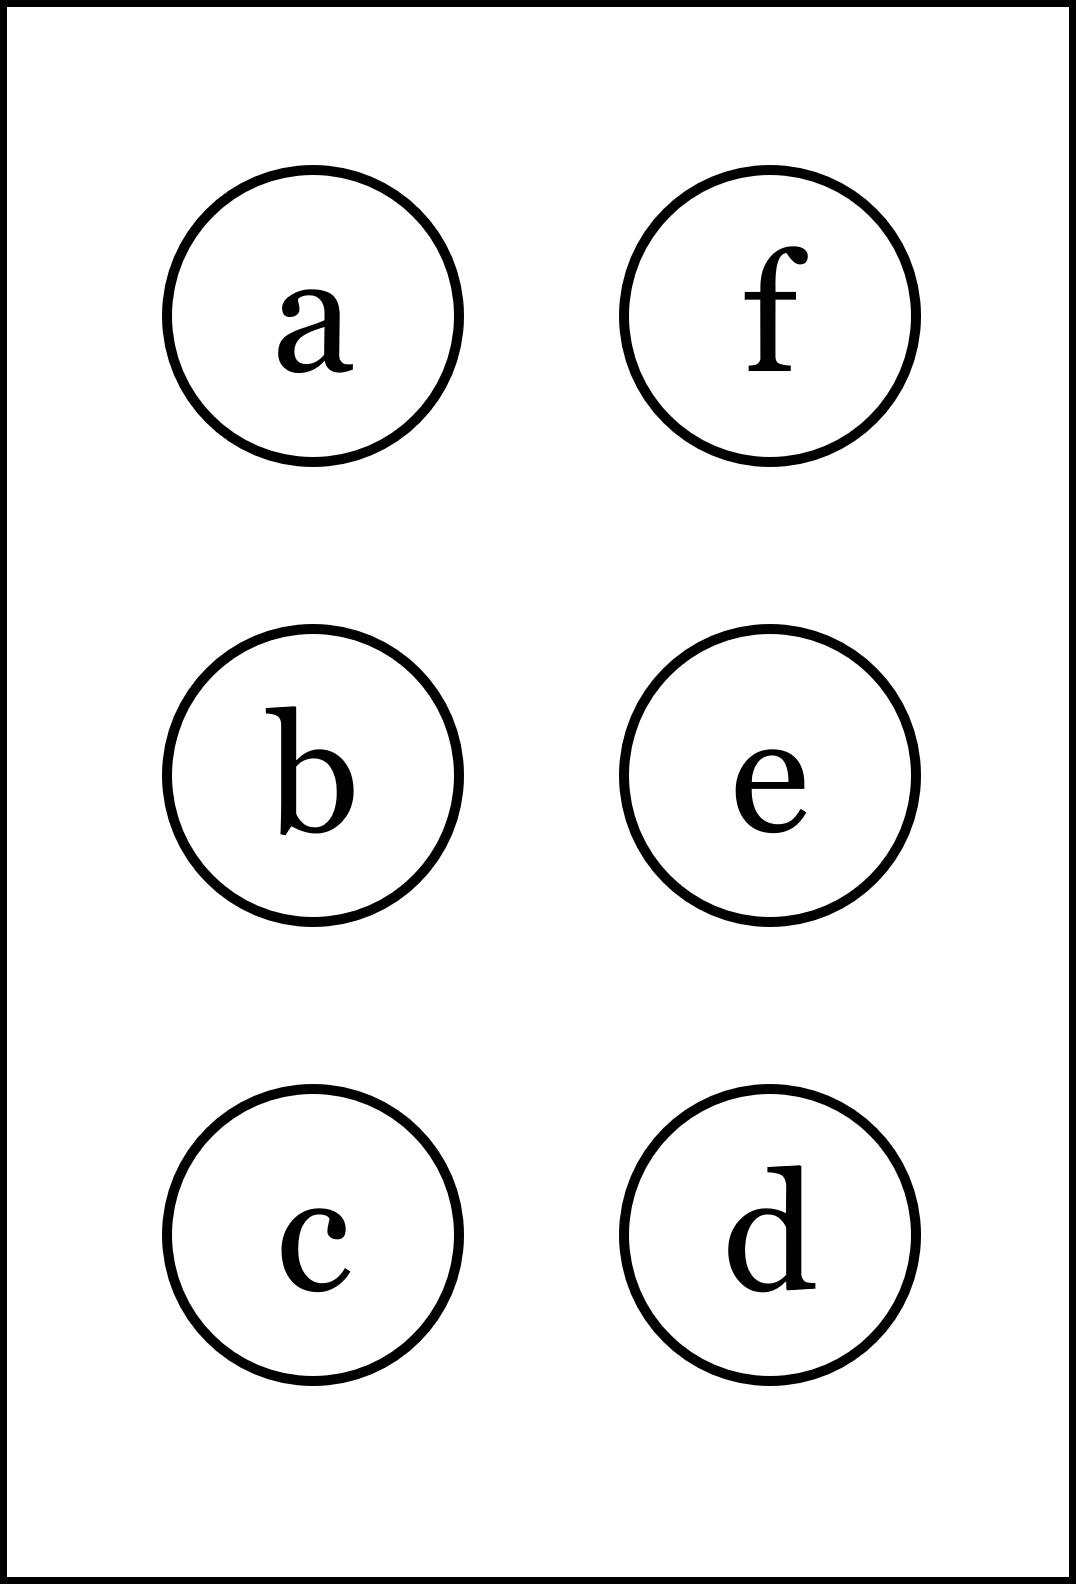
\includegraphics[height=40mm]{../images/braille.png}
{\small Písmeno Braillovej abecedy}
\end{center}
\end{minipage}
\end{center}
\end{minipage}
&
\begin{minipage}[c][99mm][t]{0.49\linewidth}
\begin{center}
\vspace{7mm}
{\huge Kubická rovnice, skupina \textit{Epsilon $\epsilon$} -\romannumeral4}\\[4.5mm]
\textit{Meno:}\phantom{xxxxxxxxxxxxxxxxxxxxxxxxxxxxxxxxxxxxxxxxxxxxxxxxxxxxxxxxxxxxxxxxx}\\[3.5mm]
\textbf{Vypočítej součet kořenů kubické rovnice.} Dvojitý kořen považuj do součtu za dva.\\Analogicky pro trojitý kořen. Pokud ti vyjde stejný výsledek jako je za otazníky, tak\\napravo obarvi příslušející kroužek načerno. \textbf{Spolu odevzdejte výsledné slovo}.\\[3mm]
\begin{minipage}{0.77\linewidth}
\begin{center}
\begin{varwidth}{\textwidth}
\begin{enumerate}
\large
\item $-x^3-x^2+30x=0$\quad \dotfill\; ???\;\dotfill \quad -1
\item $3x^3-15x^2+6x+24=0$\quad \dotfill\; ???\;\dotfill \quad -1
\item $4x^3-2x^2-34x-28=0$\quad \dotfill\; ???\;\dotfill \quad $\nicefrac{5}{2}$
\item $-8x^3-22x^2+43x+12=0$\quad \dotfill\; ???\;\dotfill \quad $\nicefrac{9}{4}$
\item \quad \dotfill\; ???\;\dotfill \quad nebarvi
\item \quad \dotfill\; ???\;\dotfill \quad nebarvi
\end{enumerate}
\end{varwidth}
\end{center}
\end{minipage}
\begin{minipage}{0.20\linewidth}
\begin{center}
{\Huge\bfseries 4.} \\[2mm]
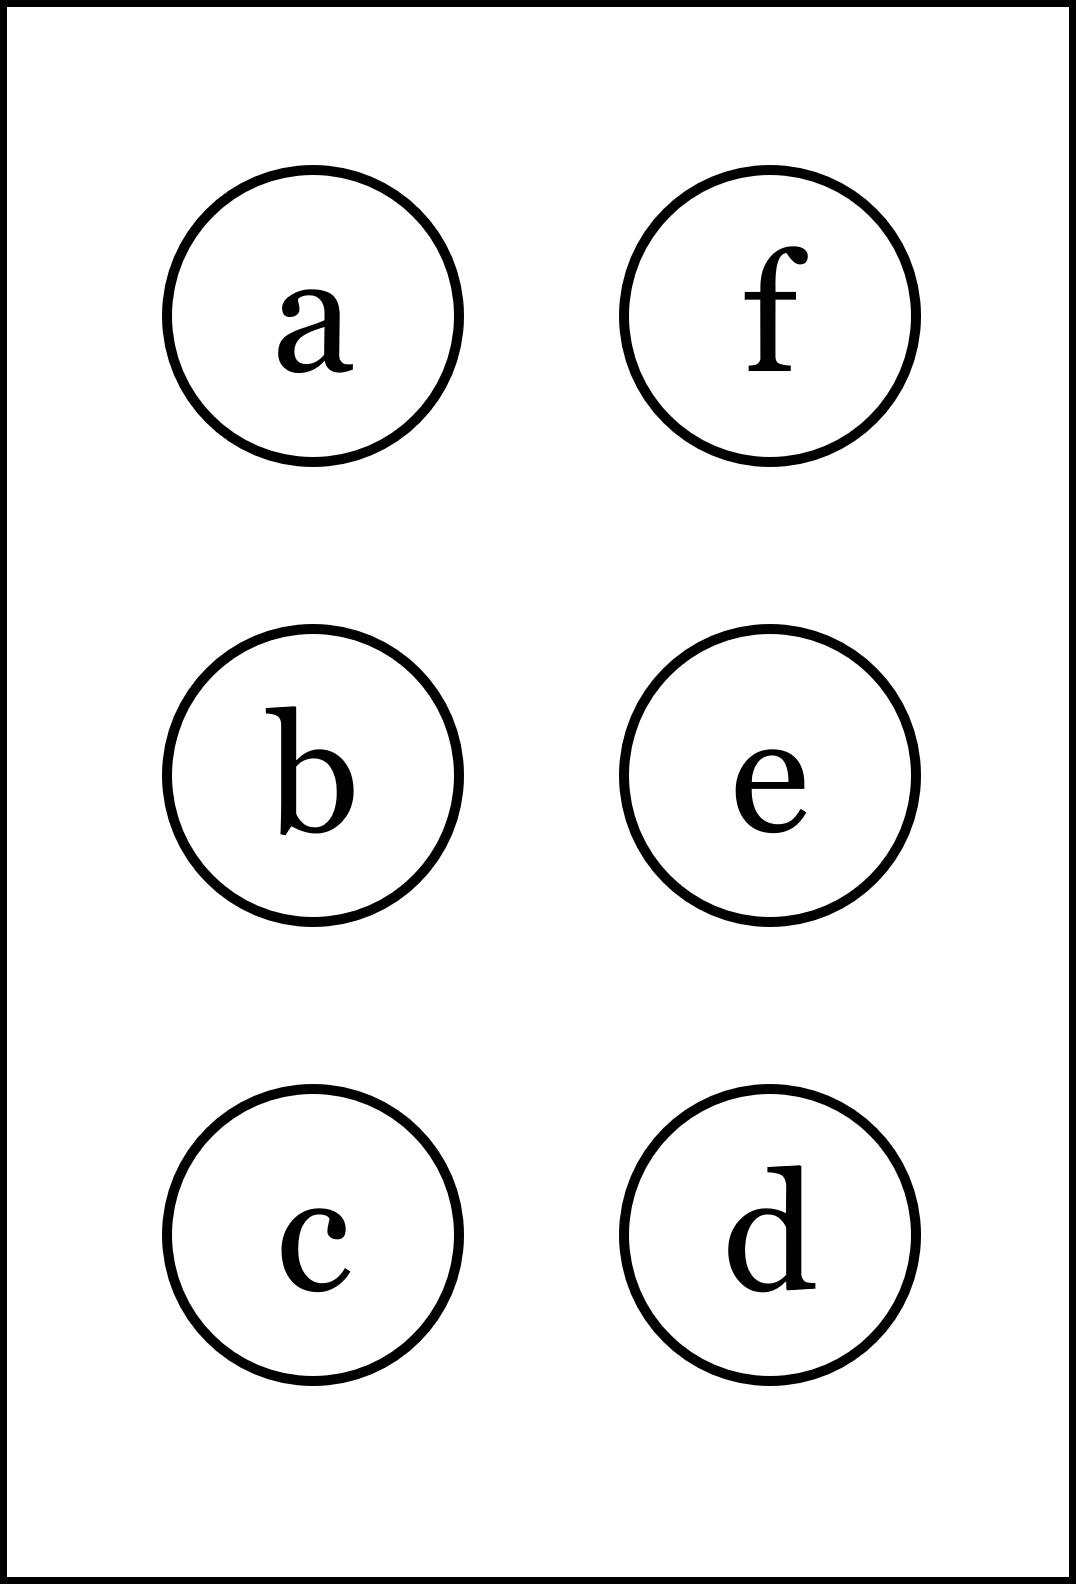
\includegraphics[height=40mm]{../images/braille.png}
{\small Písmeno Braillovej abecedy}
\end{center}
\end{minipage}
\end{center}
\end{minipage}

\end{tabular}
\begin{tikzpicture}[remember picture,overlay]\node[xshift=7mm,yshift=-100.6mm,anchor=north west] at (current page.north west){\ding{33}};\end{tikzpicture}
\begin{tikzpicture}[remember picture,overlay]\node[xshift=151.2mm,yshift=-7mm,anchor=north west,rotate=270] at (current page.north west){\ding{33}};\end{tikzpicture}
\clearpage
\thispagestyle{empty}
\begin{tabular}{c:c}
\begin{minipage}[c][99mm][t]{0.49\linewidth}
\begin{center}
\vspace{7mm}
{\huge Kubická rovnice, skupina \textit{Zeta $\zeta$} -\romannumeral1}\\[4.5mm]
\textit{Meno:}\phantom{xxxxxxxxxxxxxxxxxxxxxxxxxxxxxxxxxxxxxxxxxxxxxxxxxxxxxxxxxxxxxxxxx}\\[3.5mm]
\textbf{Vypočítej součet kořenů kubické rovnice.} Dvojitý kořen považuj do součtu za dva.\\Analogicky pro trojitý kořen. Pokud ti vyjde stejný výsledek jako je za otazníky, tak\\napravo obarvi příslušející kroužek načerno. \textbf{Spolu odevzdejte výsledné slovo}.\\[3mm]
\begin{minipage}{0.77\linewidth}
\begin{center}
\begin{varwidth}{\textwidth}
\begin{enumerate}
\large
\item $2x^3-16x^2+30x=0$\quad \dotfill\; ???\;\dotfill \quad 8
\item $-2x^3+4x^2+58x-60=0$\quad \dotfill\; ???\;\dotfill \quad 0
\item $-8x^3-7x^2+49x-6=0$\quad \dotfill\; ???\;\dotfill \quad $\nicefrac{9}{8}$
\item $12x^3+10x^2-4x-2=0$\quad \dotfill\; ???\;\dotfill \quad $\nicefrac{-5}{6}$
\item \quad \dotfill\; ???\;\dotfill \quad nebarvi
\item \quad \dotfill\; ???\;\dotfill \quad vybarvi
\end{enumerate}
\end{varwidth}
\end{center}
\end{minipage}
\begin{minipage}{0.20\linewidth}
\begin{center}
{\Huge\bfseries 1.} \\[2mm]
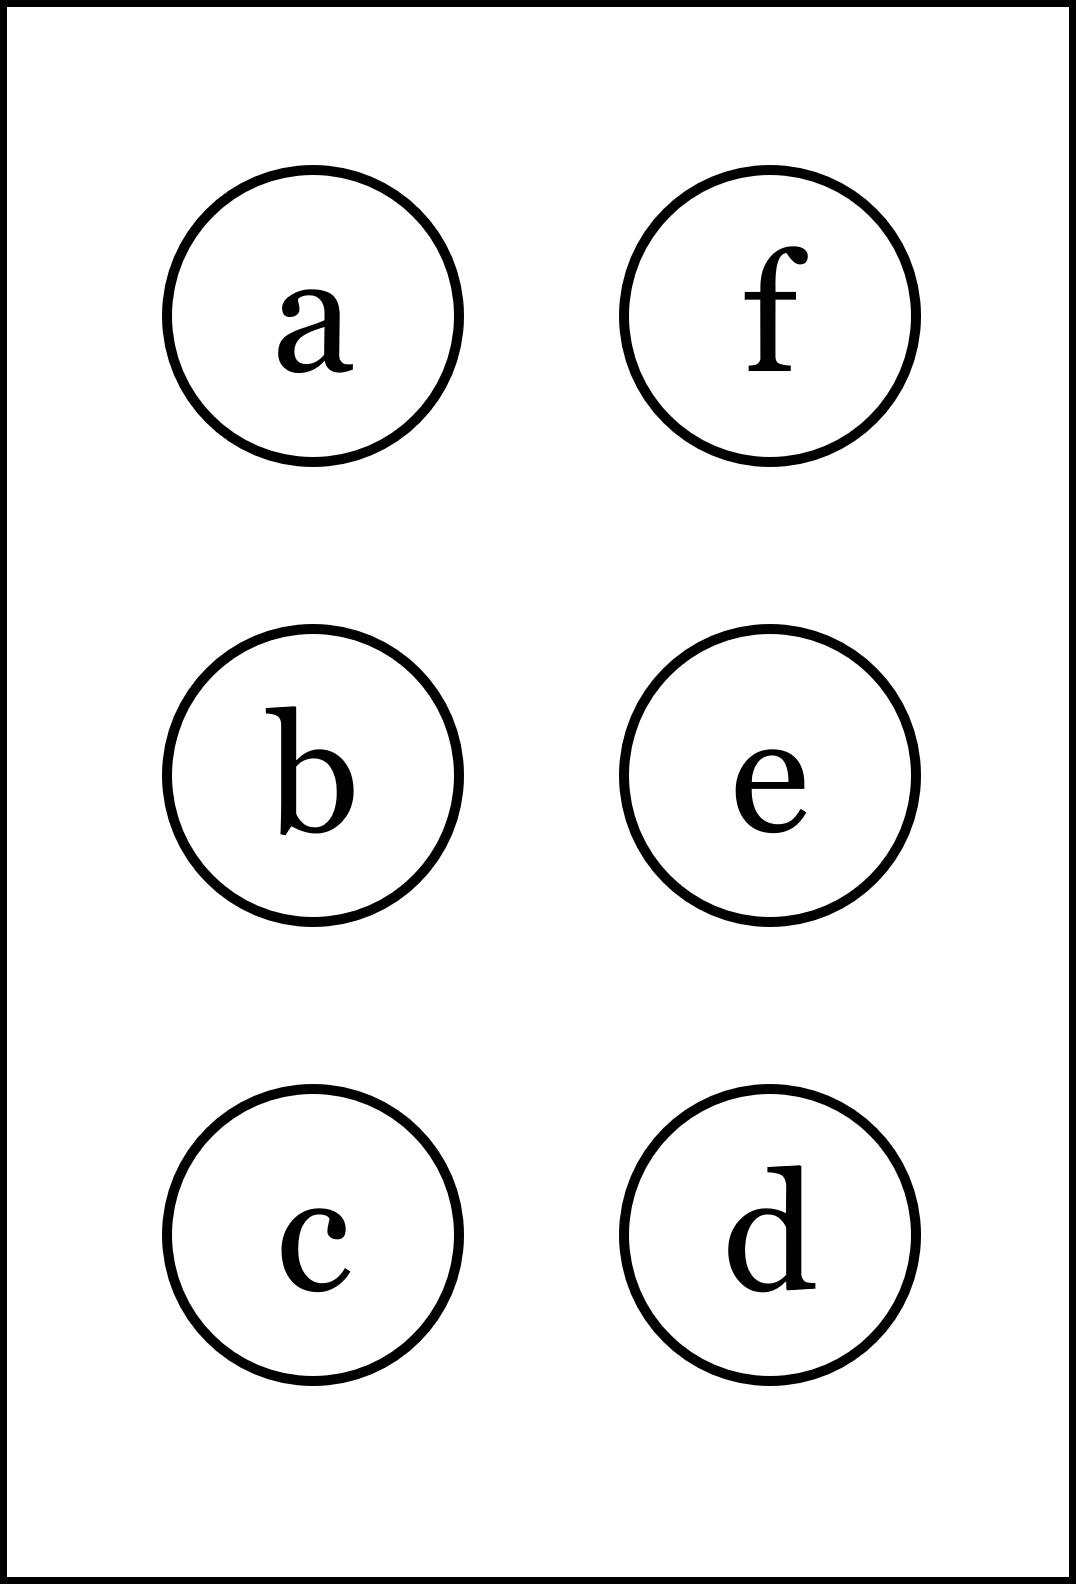
\includegraphics[height=40mm]{../images/braille.png}
{\small Písmeno Braillovej abecedy}
\end{center}
\end{minipage}
\end{center}
\end{minipage}
&
\begin{minipage}[c][99mm][t]{0.49\linewidth}
\begin{center}
\vspace{7mm}
{\huge Kubická rovnice, skupina \textit{Zeta $\zeta$} -\romannumeral2}\\[4.5mm]
\textit{Meno:}\phantom{xxxxxxxxxxxxxxxxxxxxxxxxxxxxxxxxxxxxxxxxxxxxxxxxxxxxxxxxxxxxxxxxx}\\[3.5mm]
\textbf{Vypočítej součet kořenů kubické rovnice.} Dvojitý kořen považuj do součtu za dva.\\Analogicky pro trojitý kořen. Pokud ti vyjde stejný výsledek jako je za otazníky, tak\\napravo obarvi příslušející kroužek načerno. \textbf{Spolu odevzdejte výsledné slovo}.\\[3mm]
\begin{minipage}{0.77\linewidth}
\begin{center}
\begin{varwidth}{\textwidth}
\begin{enumerate}
\large
\item $-x^3+9x^2-20x=0$\quad \dotfill\; ???\;\dotfill \quad -1
\item $-x^3-5x^2+32x-36=0$\quad \dotfill\; ???\;\dotfill \quad -9
\item $30x^3-18x^2-30x+18=0$\quad \dotfill\; ???\;\dotfill \quad $\nicefrac{3}{5}$
\item $-6x^3-19x^2+9x+36=0$\quad \dotfill\; ???\;\dotfill \quad $\nicefrac{1}{6}$
\item \quad \dotfill\; ???\;\dotfill \quad nebarvi
\item \quad \dotfill\; ???\;\dotfill \quad vybarvi
\end{enumerate}
\end{varwidth}
\end{center}
\end{minipage}
\begin{minipage}{0.20\linewidth}
\begin{center}
{\Huge\bfseries 2.} \\[2mm]
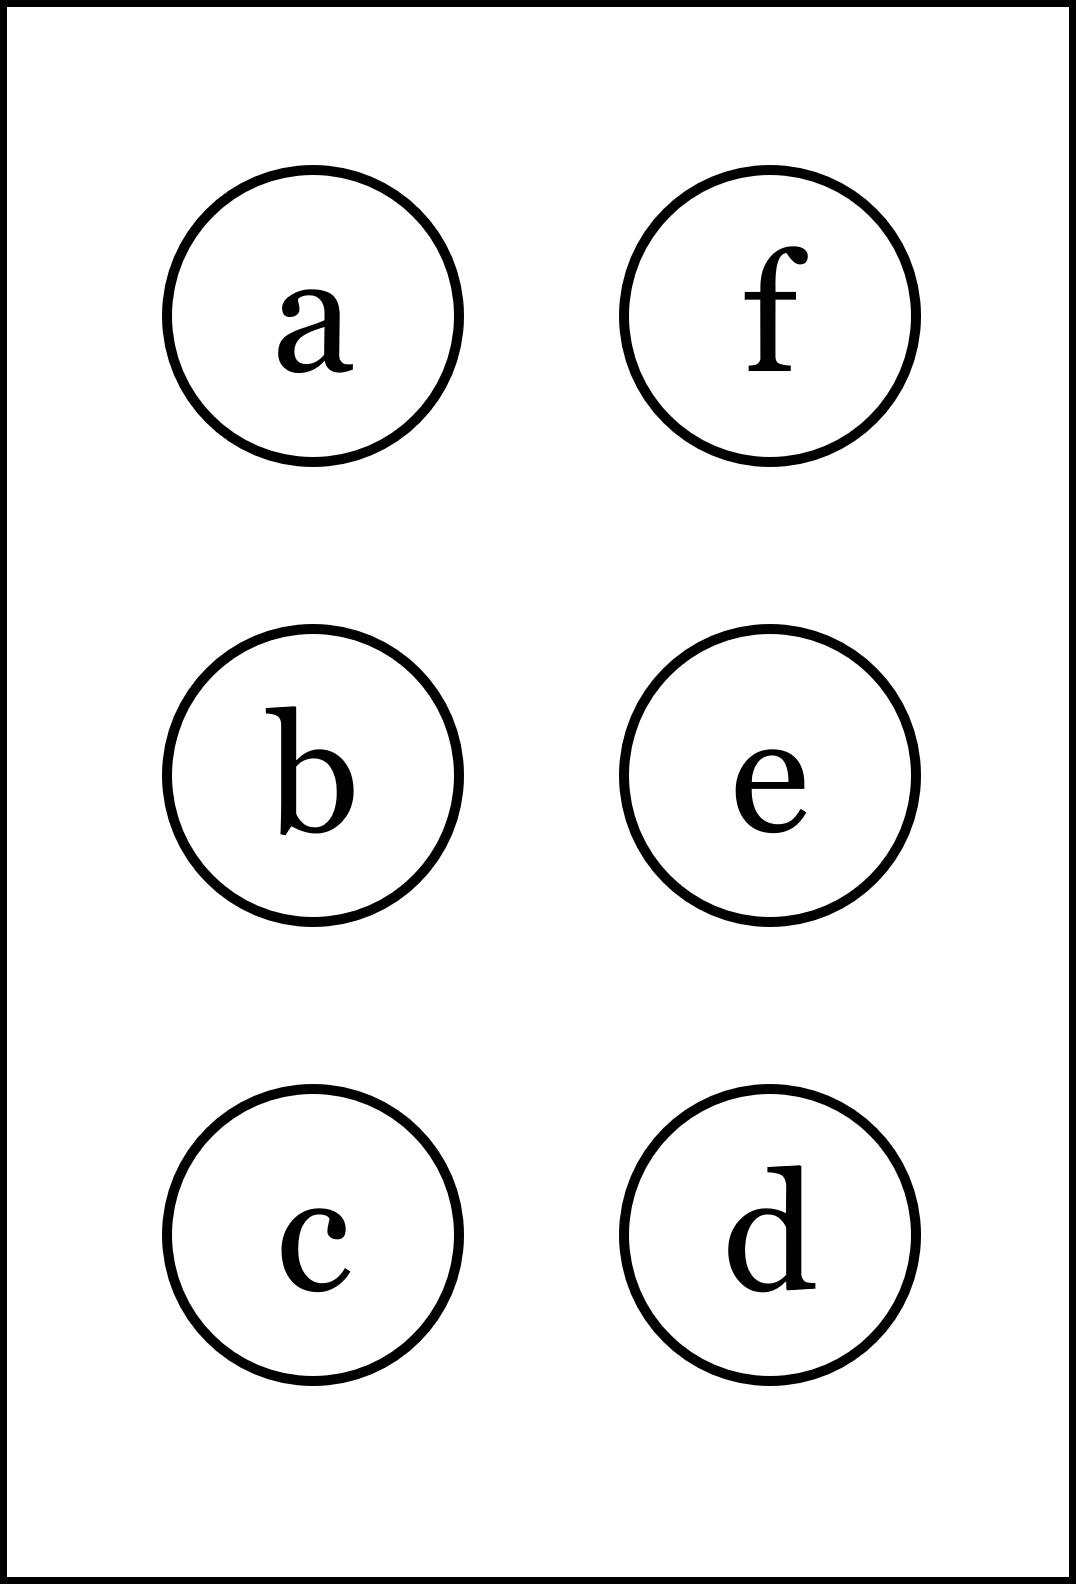
\includegraphics[height=40mm]{../images/braille.png}
{\small Písmeno Braillovej abecedy}
\end{center}
\end{minipage}
\end{center}
\end{minipage}
\\ \hdashline
\begin{minipage}[c][99mm][t]{0.49\linewidth}
\begin{center}
\vspace{7mm}
{\huge Kubická rovnice, skupina \textit{Zeta $\zeta$} -\romannumeral3}\\[4.5mm]
\textit{Meno:}\phantom{xxxxxxxxxxxxxxxxxxxxxxxxxxxxxxxxxxxxxxxxxxxxxxxxxxxxxxxxxxxxxxxxx}\\[3.5mm]
\textbf{Vypočítej součet kořenů kubické rovnice.} Dvojitý kořen považuj do součtu za dva.\\Analogicky pro trojitý kořen. Pokud ti vyjde stejný výsledek jako je za otazníky, tak\\napravo obarvi příslušející kroužek načerno. \textbf{Spolu odevzdejte výsledné slovo}.\\[3mm]
\begin{minipage}{0.77\linewidth}
\begin{center}
\begin{varwidth}{\textwidth}
\begin{enumerate}
\large
\item $-x^3-x^2+2x=0$\quad \dotfill\; ???\;\dotfill \quad -1
\item $-6x^3-6x^2+54x+54=0$\quad \dotfill\; ???\;\dotfill \quad -5
\item $54x^3+45x^2-39x-30=0$\quad \dotfill\; ???\;\dotfill \quad $\nicefrac{-5}{6}$
\item $-3x^3-5x^2+6x+8=0$\quad \dotfill\; ???\;\dotfill \quad $\nicefrac{13}{3}$
\item \quad \dotfill\; ???\;\dotfill \quad vybarvi
\item \quad \dotfill\; ???\;\dotfill \quad vybarvi
\end{enumerate}
\end{varwidth}
\end{center}
\end{minipage}
\begin{minipage}{0.20\linewidth}
\begin{center}
{\Huge\bfseries 3.} \\[2mm]
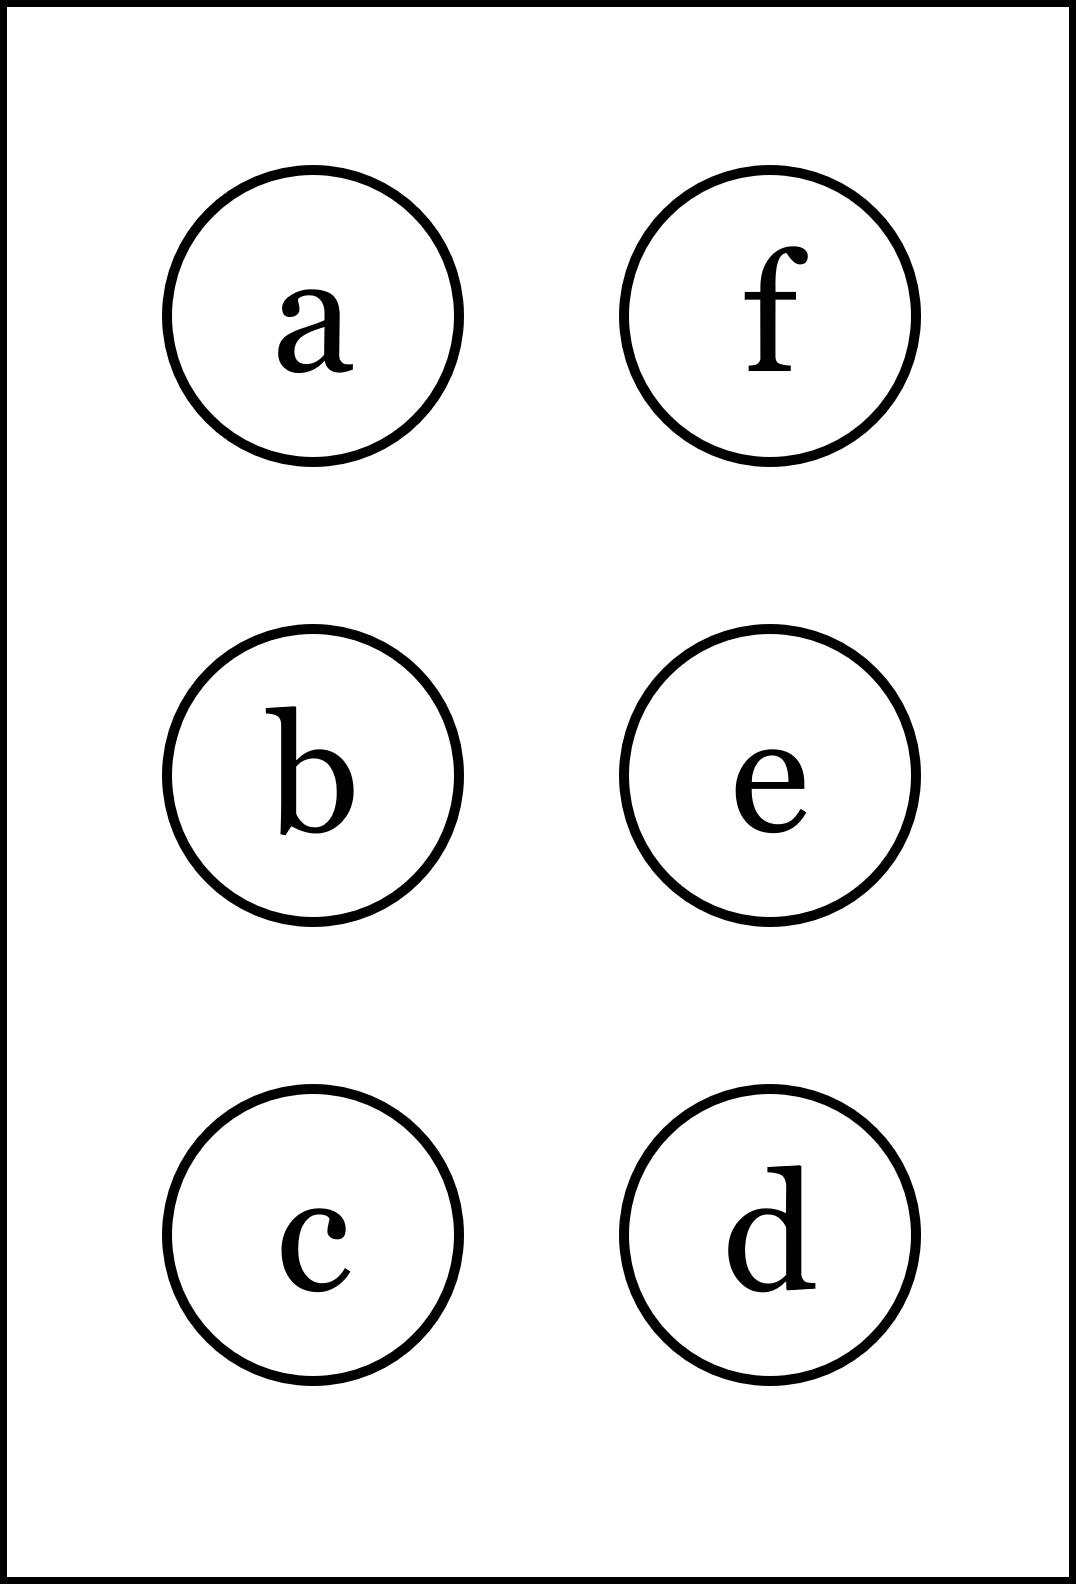
\includegraphics[height=40mm]{../images/braille.png}
{\small Písmeno Braillovej abecedy}
\end{center}
\end{minipage}
\end{center}
\end{minipage}
&
\begin{minipage}[c][99mm][t]{0.49\linewidth}
\begin{center}
\vspace{7mm}
{\huge Kubická rovnice, skupina \textit{Zeta $\zeta$} -\romannumeral4}\\[4.5mm]
\textit{Meno:}\phantom{xxxxxxxxxxxxxxxxxxxxxxxxxxxxxxxxxxxxxxxxxxxxxxxxxxxxxxxxxxxxxxxxx}\\[3.5mm]
\textbf{Vypočítej součet kořenů kubické rovnice.} Dvojitý kořen považuj do součtu za dva.\\Analogicky pro trojitý kořen. Pokud ti vyjde stejný výsledek jako je za otazníky, tak\\napravo obarvi příslušející kroužek načerno. \textbf{Spolu odevzdejte výsledné slovo}.\\[3mm]
\begin{minipage}{0.77\linewidth}
\begin{center}
\begin{varwidth}{\textwidth}
\begin{enumerate}
\large
\item $x^3-12x^2+35x=0$\quad \dotfill\; ???\;\dotfill \quad 12
\item $2x^3-14x^2-2x+14=0$\quad \dotfill\; ???\;\dotfill \quad 5
\item $-24x^3-66x^2-60x-18=0$\quad \dotfill\; ???\;\dotfill \quad $\nicefrac{5}{4}$
\item $-5x^3+21x^2+50x+24=0$\quad \dotfill\; ???\;\dotfill \quad $\nicefrac{-29}{5}$
\item \quad \dotfill\; ???\;\dotfill \quad nebarvi
\item \quad \dotfill\; ???\;\dotfill \quad nebarvi
\end{enumerate}
\end{varwidth}
\end{center}
\end{minipage}
\begin{minipage}{0.20\linewidth}
\begin{center}
{\Huge\bfseries 4.} \\[2mm]
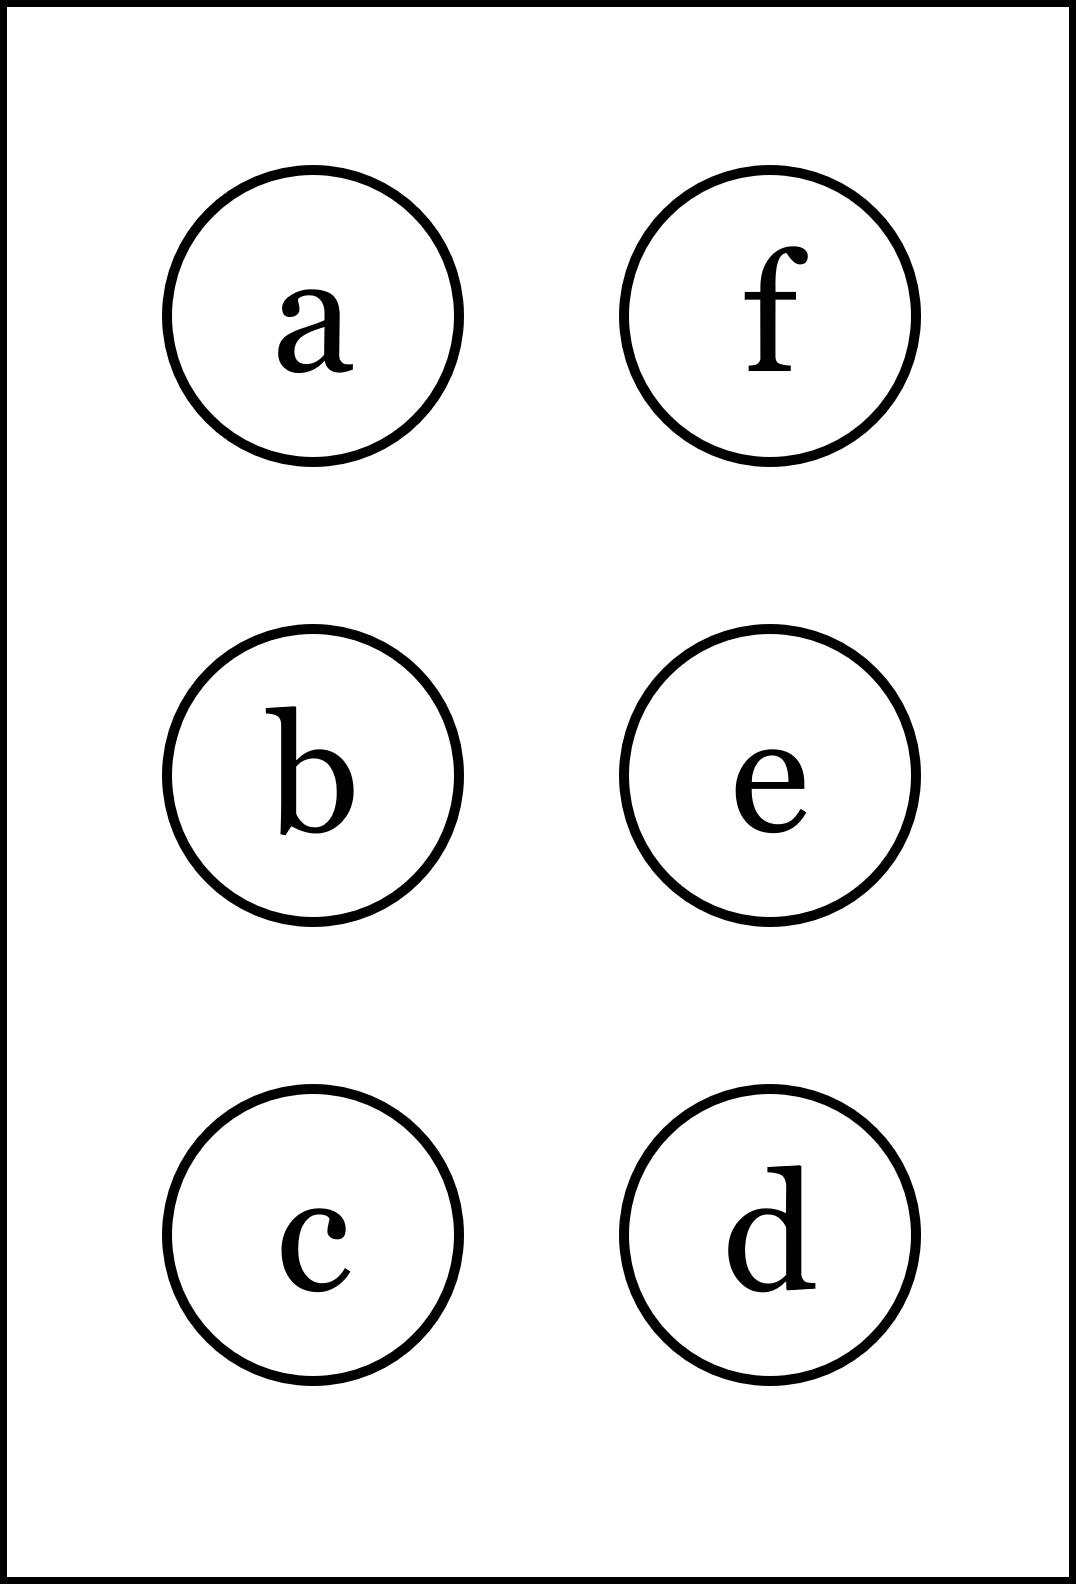
\includegraphics[height=40mm]{../images/braille.png}
{\small Písmeno Braillovej abecedy}
\end{center}
\end{minipage}
\end{center}
\end{minipage}

\end{tabular}
\begin{tikzpicture}[remember picture,overlay]\node[xshift=7mm,yshift=-100.6mm,anchor=north west] at (current page.north west){\ding{33}};\end{tikzpicture}
\begin{tikzpicture}[remember picture,overlay]\node[xshift=151.2mm,yshift=-7mm,anchor=north west,rotate=270] at (current page.north west){\ding{33}};\end{tikzpicture}
\clearpage
\thispagestyle{empty}
\begin{tabular}{c:c}
\begin{minipage}[c][99mm][t]{0.49\linewidth}
\begin{center}
\vspace{7mm}
{\huge Kubická rovnice, skupina \textit{Eta $\eta$} -\romannumeral1}\\[4.5mm]
\textit{Meno:}\phantom{xxxxxxxxxxxxxxxxxxxxxxxxxxxxxxxxxxxxxxxxxxxxxxxxxxxxxxxxxxxxxxxxx}\\[3.5mm]
\textbf{Vypočítej součet kořenů kubické rovnice.} Dvojitý kořen považuj do součtu za dva.\\Analogicky pro trojitý kořen. Pokud ti vyjde stejný výsledek jako je za otazníky, tak\\napravo obarvi příslušející kroužek načerno. \textbf{Spolu odevzdejte výsledné slovo}.\\[3mm]
\begin{minipage}{0.77\linewidth}
\begin{center}
\begin{varwidth}{\textwidth}
\begin{enumerate}
\large
\item $x^3+4x^2-21x=0$\quad \dotfill\; ???\;\dotfill \quad -4
\item $3x^3-9x-6=0$\quad \dotfill\; ???\;\dotfill \quad 0
\item $-24x^3-48x^2-6x+18=0$\quad \dotfill\; ???\;\dotfill \quad 1
\item $-30x^3+26x^2+6x-2=0$\quad \dotfill\; ???\;\dotfill \quad $\nicefrac{-23}{15}$
\item \quad \dotfill\; ???\;\dotfill \quad nebarvi
\item \quad \dotfill\; ???\;\dotfill \quad vybarvi
\end{enumerate}
\end{varwidth}
\end{center}
\end{minipage}
\begin{minipage}{0.20\linewidth}
\begin{center}
{\Huge\bfseries 1.} \\[2mm]
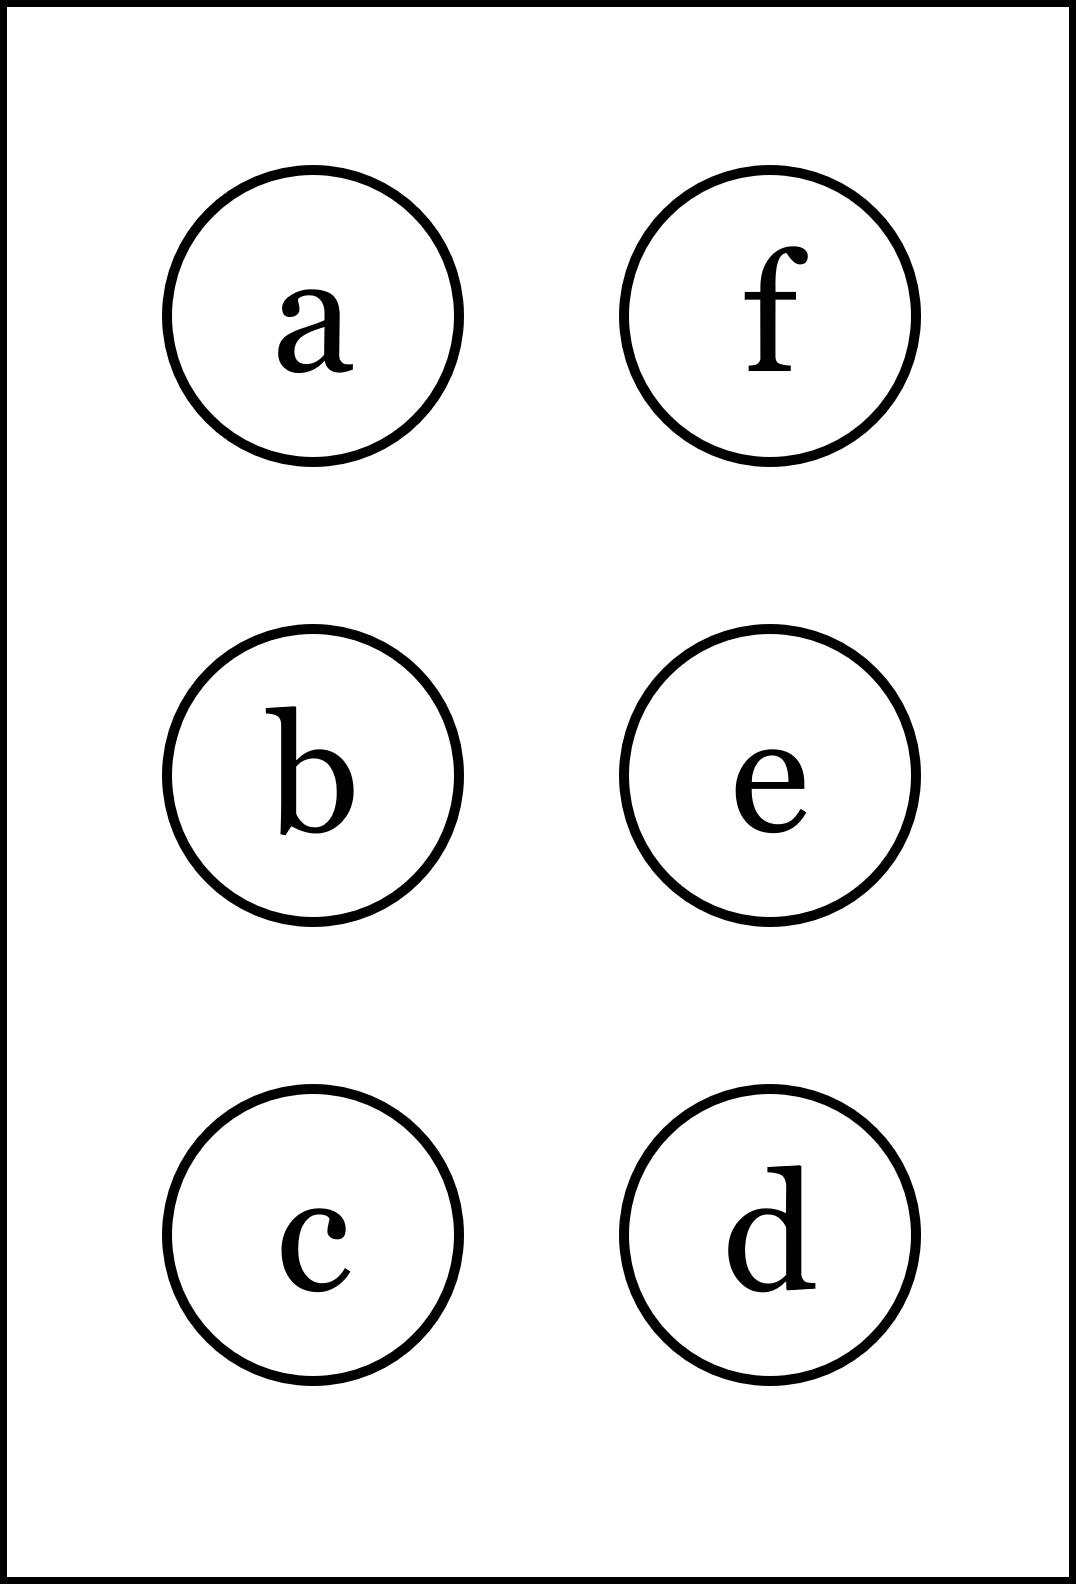
\includegraphics[height=40mm]{../images/braille.png}
{\small Písmeno Braillovej abecedy}
\end{center}
\end{minipage}
\end{center}
\end{minipage}
&
\begin{minipage}[c][99mm][t]{0.49\linewidth}
\begin{center}
\vspace{7mm}
{\huge Kubická rovnice, skupina \textit{Eta $\eta$} -\romannumeral2}\\[4.5mm]
\textit{Meno:}\phantom{xxxxxxxxxxxxxxxxxxxxxxxxxxxxxxxxxxxxxxxxxxxxxxxxxxxxxxxxxxxxxxxxx}\\[3.5mm]
\textbf{Vypočítej součet kořenů kubické rovnice.} Dvojitý kořen považuj do součtu za dva.\\Analogicky pro trojitý kořen. Pokud ti vyjde stejný výsledek jako je za otazníky, tak\\napravo obarvi příslušející kroužek načerno. \textbf{Spolu odevzdejte výsledné slovo}.\\[3mm]
\begin{minipage}{0.77\linewidth}
\begin{center}
\begin{varwidth}{\textwidth}
\begin{enumerate}
\large
\item $-2x^3-8x^2+10x=0$\quad \dotfill\; ???\;\dotfill \quad -4
\item $-6x^3-24x^2+6x+24=0$\quad \dotfill\; ???\;\dotfill \quad -2
\item $42x^3-21x^2-42x+21=0$\quad \dotfill\; ???\;\dotfill \quad $\nicefrac{1}{2}$
\item $-12x^3+35x^2+49x+12=0$\quad \dotfill\; ???\;\dotfill \quad $\nicefrac{-53}{12}$
\item \quad \dotfill\; ???\;\dotfill \quad vybarvi
\item \quad \dotfill\; ???\;\dotfill \quad nebarvi
\end{enumerate}
\end{varwidth}
\end{center}
\end{minipage}
\begin{minipage}{0.20\linewidth}
\begin{center}
{\Huge\bfseries 2.} \\[2mm]
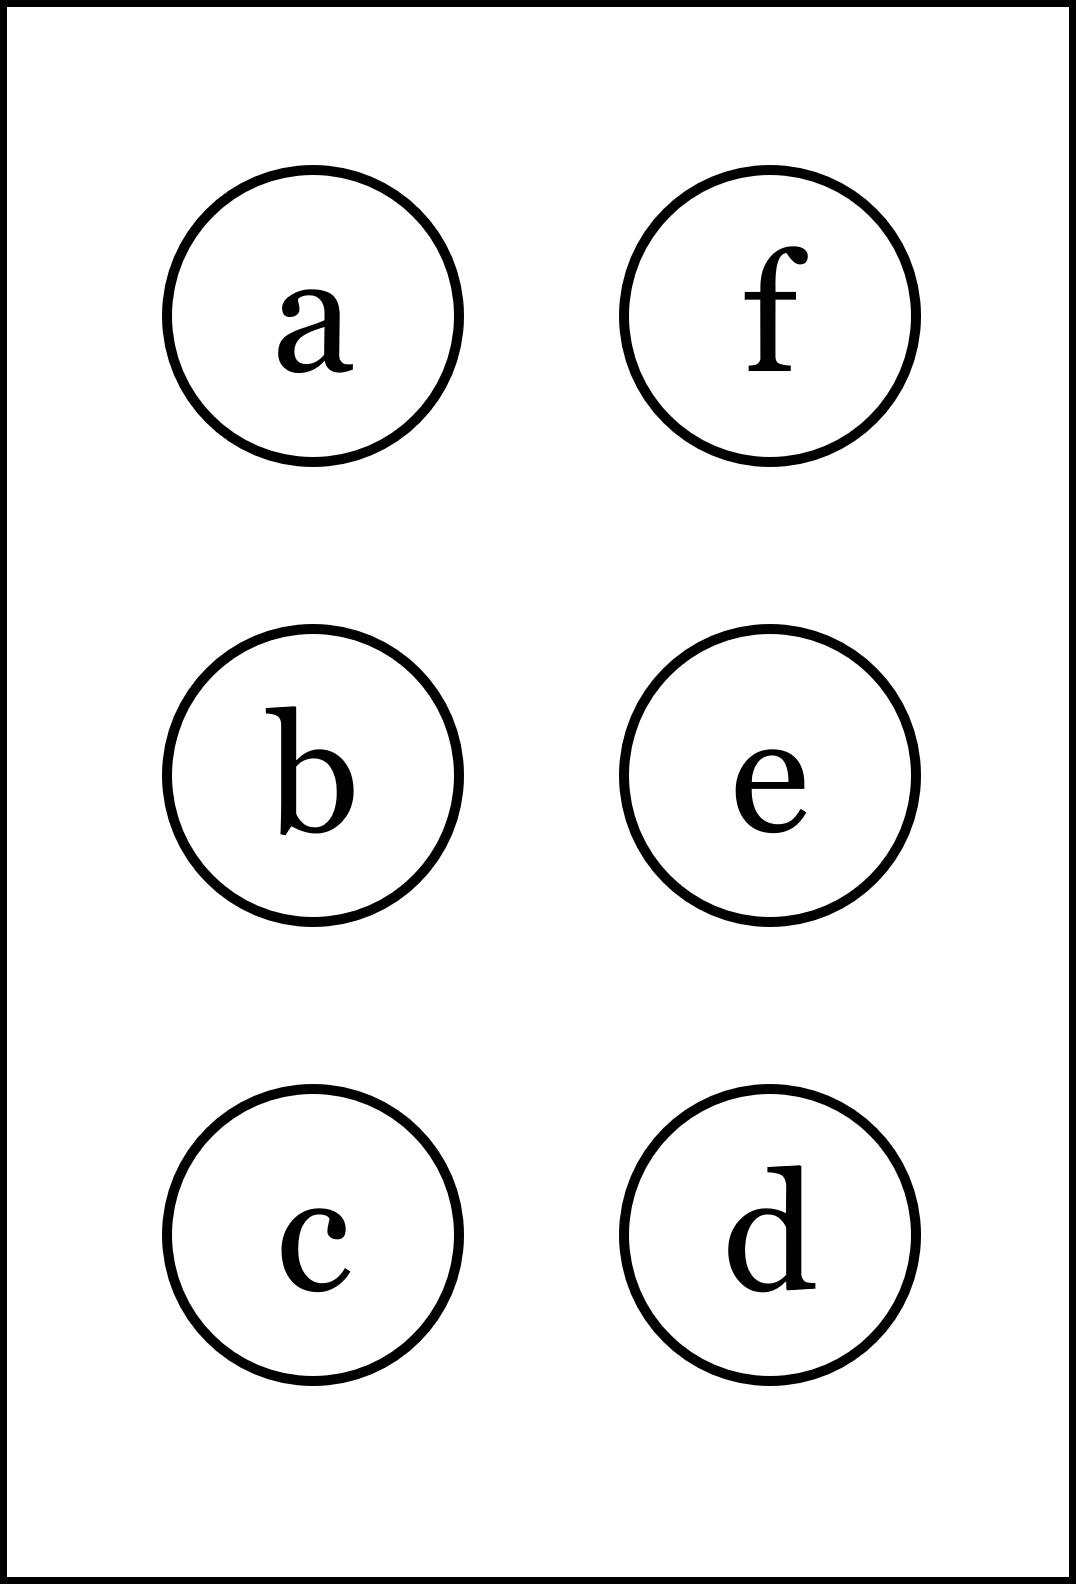
\includegraphics[height=40mm]{../images/braille.png}
{\small Písmeno Braillovej abecedy}
\end{center}
\end{minipage}
\end{center}
\end{minipage}
\\ \hdashline
\begin{minipage}[c][99mm][t]{0.49\linewidth}
\begin{center}
\vspace{7mm}
{\huge Kubická rovnice, skupina \textit{Eta $\eta$} -\romannumeral3}\\[4.5mm]
\textit{Meno:}\phantom{xxxxxxxxxxxxxxxxxxxxxxxxxxxxxxxxxxxxxxxxxxxxxxxxxxxxxxxxxxxxxxxxx}\\[3.5mm]
\textbf{Vypočítej součet kořenů kubické rovnice.} Dvojitý kořen považuj do součtu za dva.\\Analogicky pro trojitý kořen. Pokud ti vyjde stejný výsledek jako je za otazníky, tak\\napravo obarvi příslušející kroužek načerno. \textbf{Spolu odevzdejte výsledné slovo}.\\[3mm]
\begin{minipage}{0.77\linewidth}
\begin{center}
\begin{varwidth}{\textwidth}
\begin{enumerate}
\large
\item $8x^3-8x^2-48x=0$\quad \dotfill\; ???\;\dotfill \quad -5
\item $x^3-6x^2-x+6=0$\quad \dotfill\; ???\;\dotfill \quad 6
\item $-4x^3-34x^2-86x-56=0$\quad \dotfill\; ???\;\dotfill \quad $\nicefrac{-17}{2}$
\item $x^3+8x^2+11x-20=0$\quad \dotfill\; ???\;\dotfill \quad 10
\item \quad \dotfill\; ???\;\dotfill \quad vybarvi
\item \quad \dotfill\; ???\;\dotfill \quad vybarvi
\end{enumerate}
\end{varwidth}
\end{center}
\end{minipage}
\begin{minipage}{0.20\linewidth}
\begin{center}
{\Huge\bfseries 3.} \\[2mm]
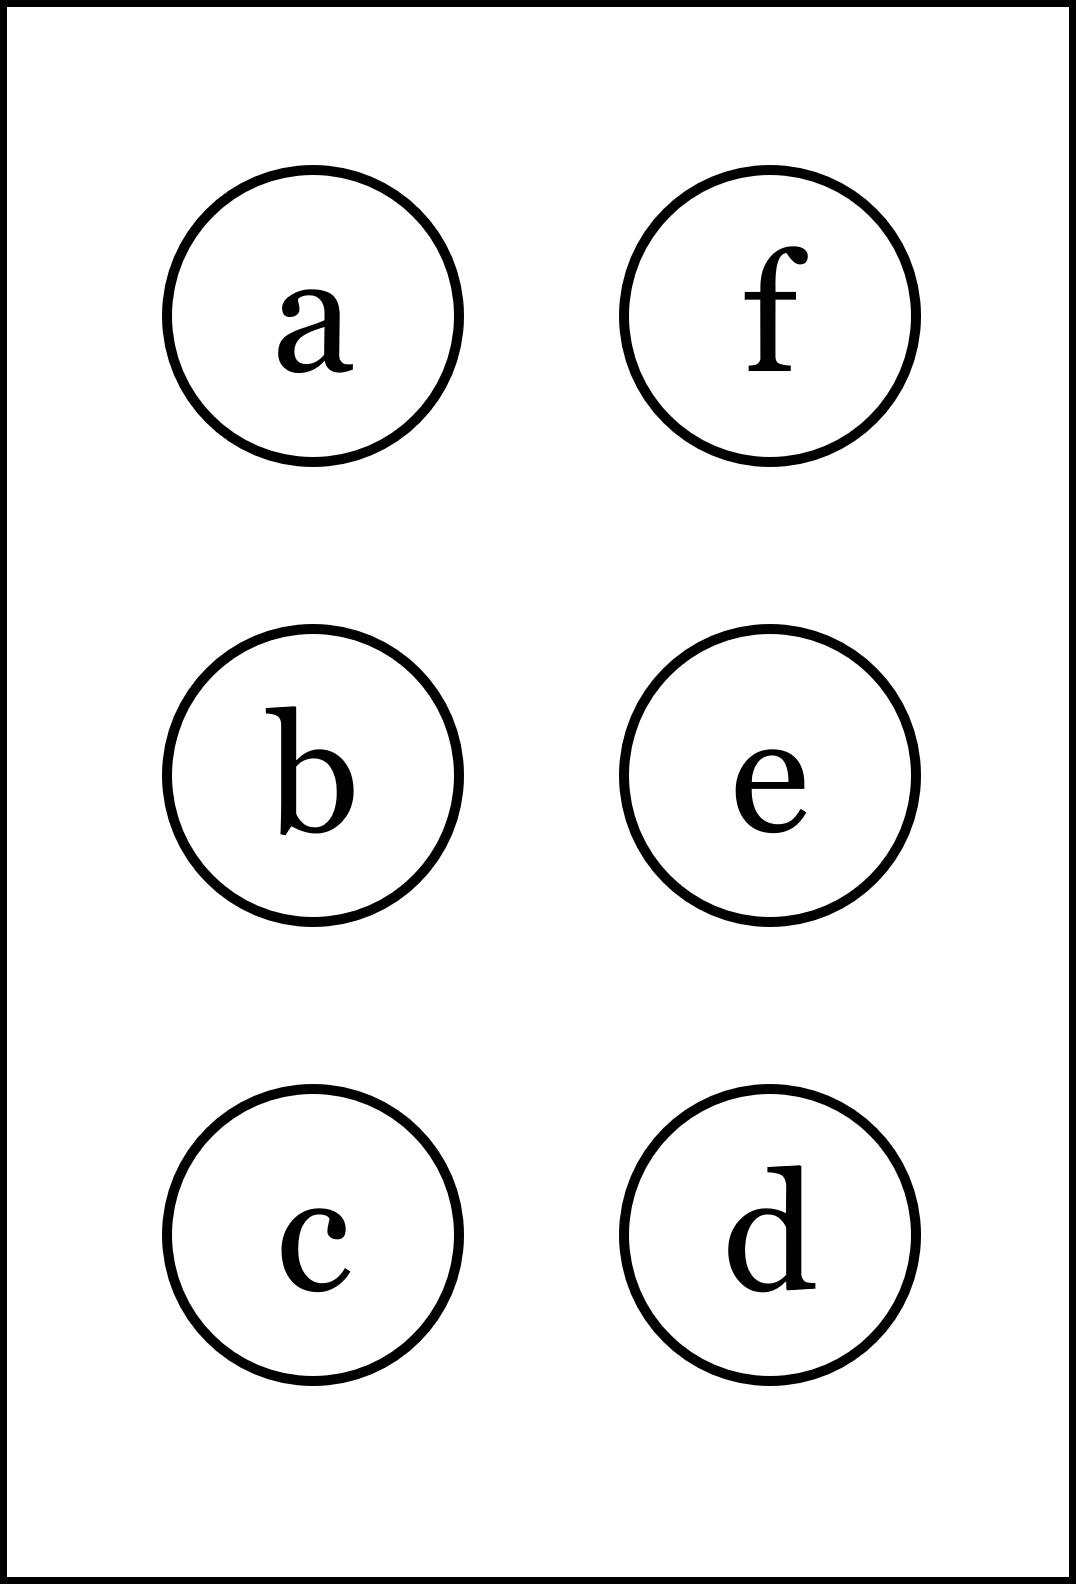
\includegraphics[height=40mm]{../images/braille.png}
{\small Písmeno Braillovej abecedy}
\end{center}
\end{minipage}
\end{center}
\end{minipage}
&
\begin{minipage}[c][99mm][t]{0.49\linewidth}
\begin{center}
\vspace{7mm}
{\huge Kubická rovnice, skupina \textit{Eta $\eta$} -\romannumeral4}\\[4.5mm]
\textit{Meno:}\phantom{xxxxxxxxxxxxxxxxxxxxxxxxxxxxxxxxxxxxxxxxxxxxxxxxxxxxxxxxxxxxxxxxx}\\[3.5mm]
\textbf{Vypočítej součet kořenů kubické rovnice.} Dvojitý kořen považuj do součtu za dva.\\Analogicky pro trojitý kořen. Pokud ti vyjde stejný výsledek jako je za otazníky, tak\\napravo obarvi příslušející kroužek načerno. \textbf{Spolu odevzdejte výsledné slovo}.\\[3mm]
\begin{minipage}{0.77\linewidth}
\begin{center}
\begin{varwidth}{\textwidth}
\begin{enumerate}
\large
\item $-x^3+4x=0$\quad \dotfill\; ???\;\dotfill \quad 0
\item $x^3+6x^2+11x+6=0$\quad \dotfill\; ???\;\dotfill \quad 0
\item $14x^3+2x^2-14x-2=0$\quad \dotfill\; ???\;\dotfill \quad $\nicefrac{-1}{7}$
\item $-7x^3-12x^2+60x-16=0$\quad \dotfill\; ???\;\dotfill \quad $\nicefrac{-40}{7}$
\item \quad \dotfill\; ???\;\dotfill \quad vybarvi
\item \quad \dotfill\; ???\;\dotfill \quad nebarvi
\end{enumerate}
\end{varwidth}
\end{center}
\end{minipage}
\begin{minipage}{0.20\linewidth}
\begin{center}
{\Huge\bfseries 4.} \\[2mm]
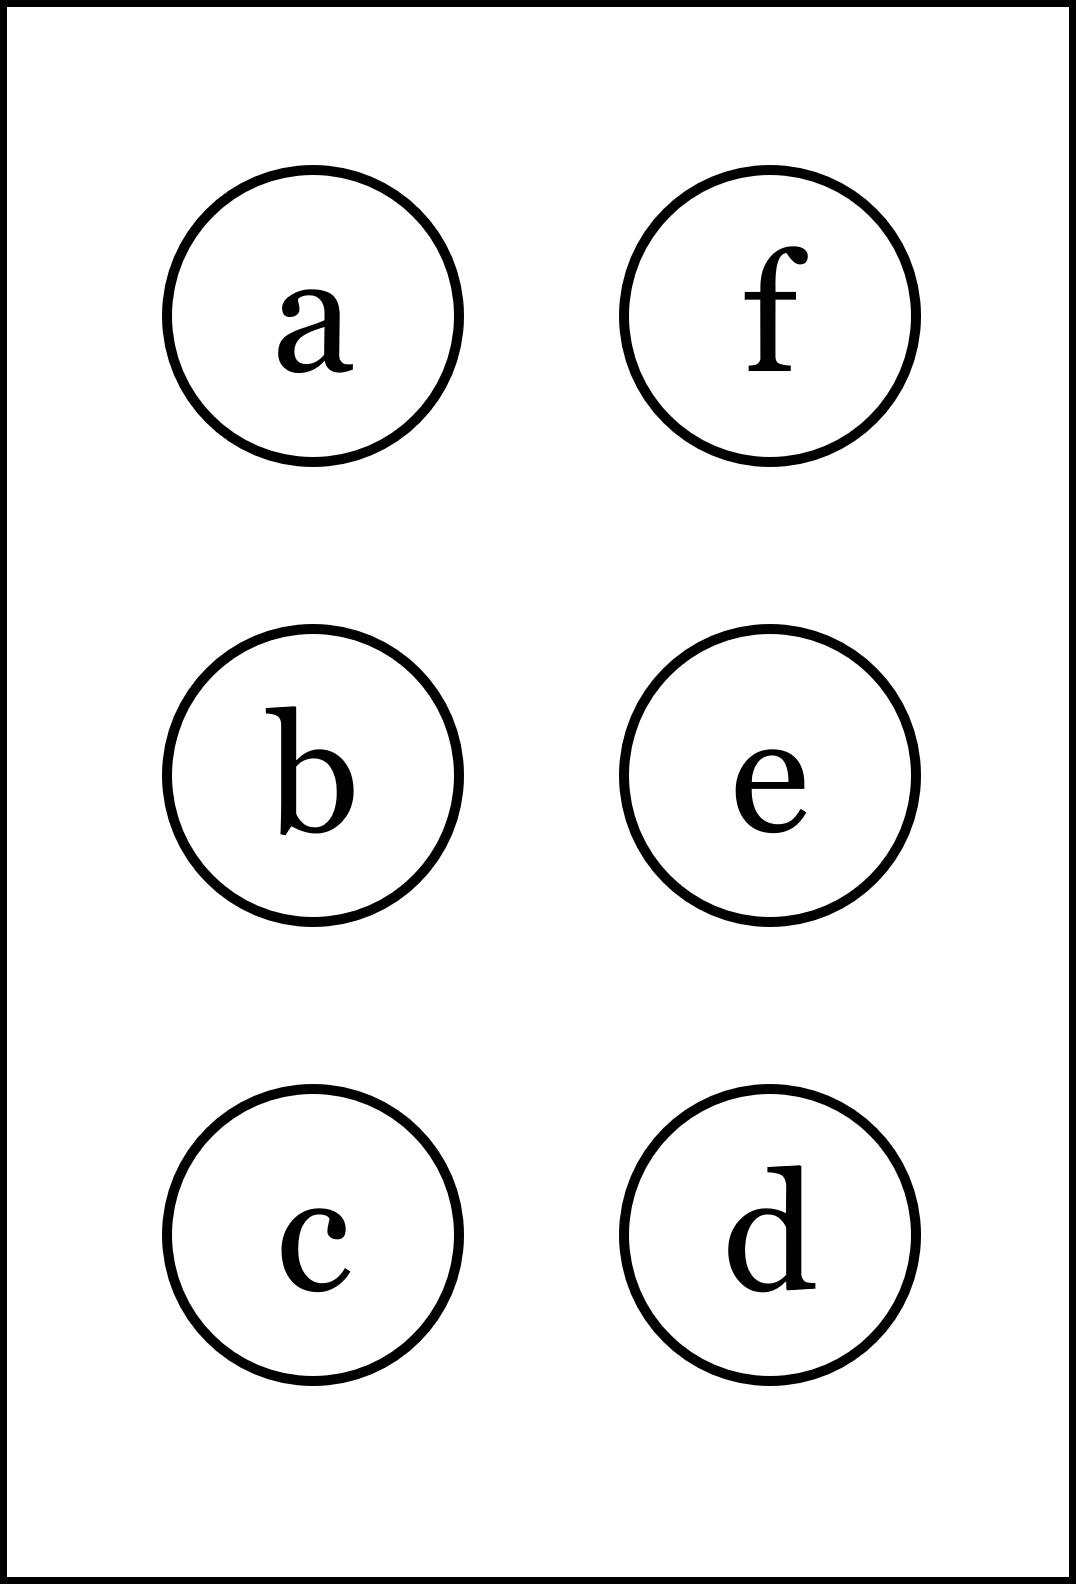
\includegraphics[height=40mm]{../images/braille.png}
{\small Písmeno Braillovej abecedy}
\end{center}
\end{minipage}
\end{center}
\end{minipage}

\end{tabular}
\begin{tikzpicture}[remember picture,overlay]\node[xshift=7mm,yshift=-100.6mm,anchor=north west] at (current page.north west){\ding{33}};\end{tikzpicture}
\begin{tikzpicture}[remember picture,overlay]\node[xshift=151.2mm,yshift=-7mm,anchor=north west,rotate=270] at (current page.north west){\ding{33}};\end{tikzpicture}
\clearpage
\thispagestyle{empty}
\begin{tabular}{c:c}
\begin{minipage}[c][99mm][t]{0.49\linewidth}
\begin{center}
\vspace{7mm}
{\huge Kubická rovnice, skupina \textit{Theta $\theta$} -\romannumeral1}\\[4.5mm]
\textit{Meno:}\phantom{xxxxxxxxxxxxxxxxxxxxxxxxxxxxxxxxxxxxxxxxxxxxxxxxxxxxxxxxxxxxxxxxx}\\[3.5mm]
\textbf{Vypočítej součet kořenů kubické rovnice.} Dvojitý kořen považuj do součtu za dva.\\Analogicky pro trojitý kořen. Pokud ti vyjde stejný výsledek jako je za otazníky, tak\\napravo obarvi příslušející kroužek načerno. \textbf{Spolu odevzdejte výsledné slovo}.\\[3mm]
\begin{minipage}{0.77\linewidth}
\begin{center}
\begin{varwidth}{\textwidth}
\begin{enumerate}
\large
\item $-2x^3-10x^2+12x=0$\quad \dotfill\; ???\;\dotfill \quad -5
\item $-x^3-x^2+32x+60=0$\quad \dotfill\; ???\;\dotfill \quad 3
\item $-5x^3+15x+10=0$\quad \dotfill\; ???\;\dotfill \quad -2
\item $8x^3-60x^2+24x+28=0$\quad \dotfill\; ???\;\dotfill \quad $\nicefrac{11}{2}$
\item \quad \dotfill\; ???\;\dotfill \quad nebarvi
\item \quad \dotfill\; ???\;\dotfill \quad nebarvi
\end{enumerate}
\end{varwidth}
\end{center}
\end{minipage}
\begin{minipage}{0.20\linewidth}
\begin{center}
{\Huge\bfseries 1.} \\[2mm]
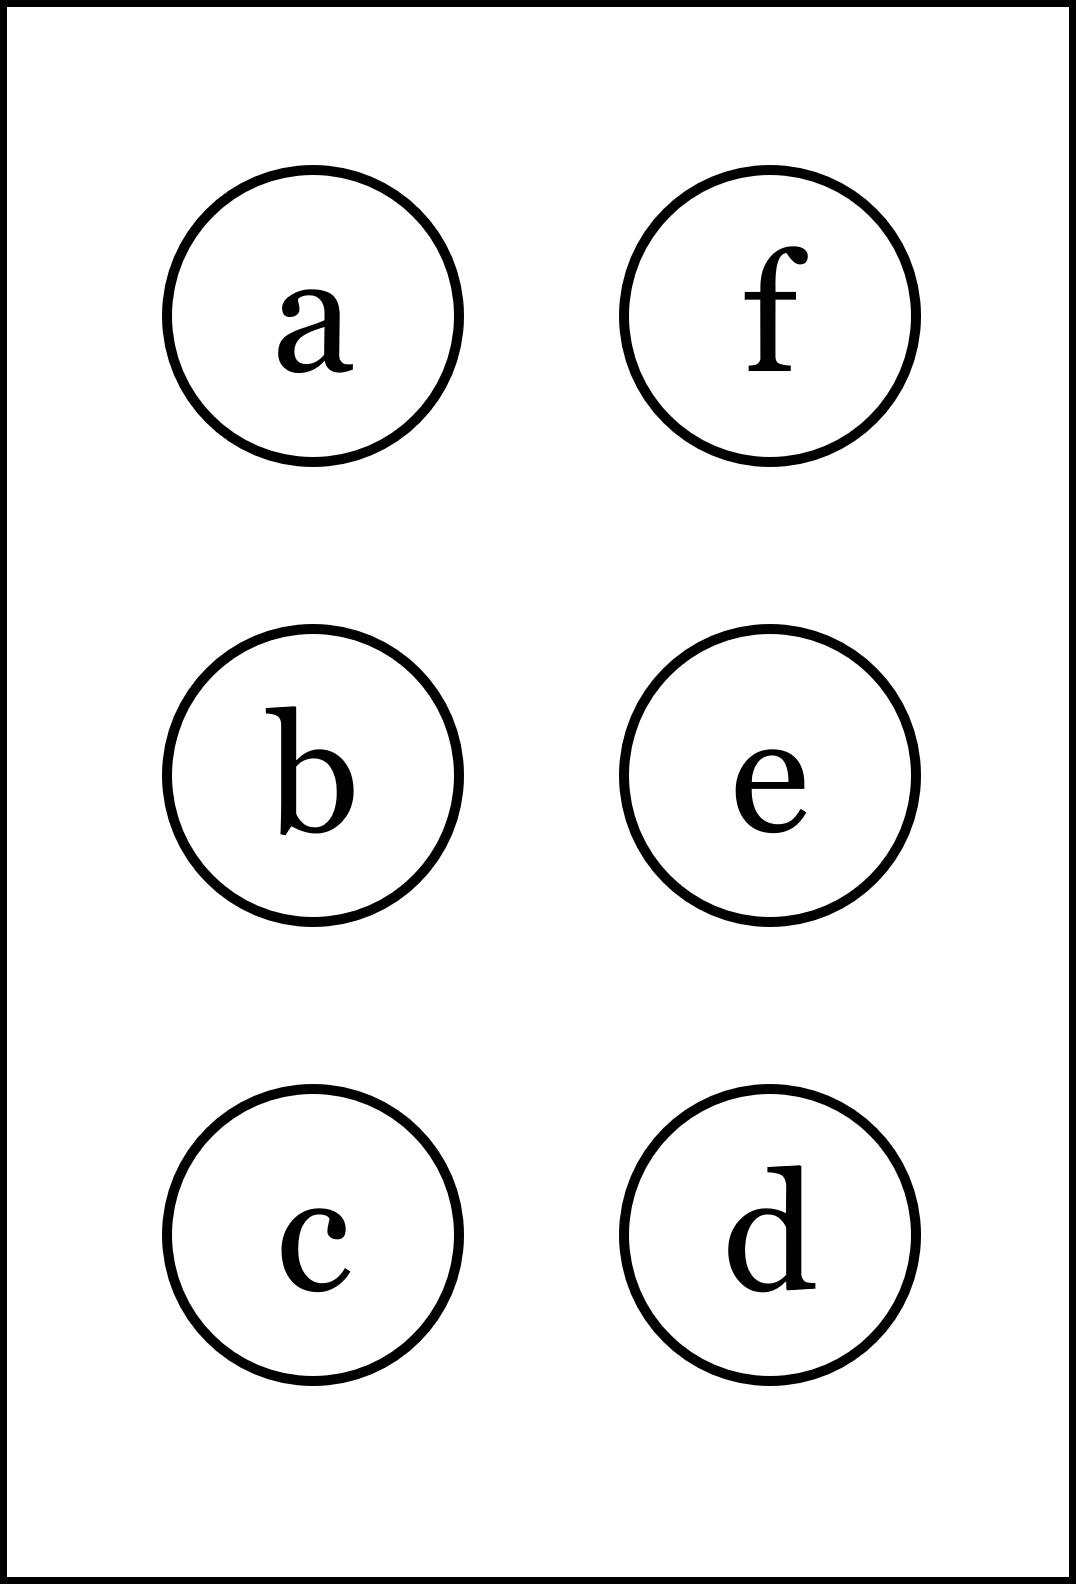
\includegraphics[height=40mm]{../images/braille.png}
{\small Písmeno Braillovej abecedy}
\end{center}
\end{minipage}
\end{center}
\end{minipage}
&
\begin{minipage}[c][99mm][t]{0.49\linewidth}
\begin{center}
\vspace{7mm}
{\huge Kubická rovnice, skupina \textit{Theta $\theta$} -\romannumeral2}\\[4.5mm]
\textit{Meno:}\phantom{xxxxxxxxxxxxxxxxxxxxxxxxxxxxxxxxxxxxxxxxxxxxxxxxxxxxxxxxxxxxxxxxx}\\[3.5mm]
\textbf{Vypočítej součet kořenů kubické rovnice.} Dvojitý kořen považuj do součtu za dva.\\Analogicky pro trojitý kořen. Pokud ti vyjde stejný výsledek jako je za otazníky, tak\\napravo obarvi příslušející kroužek načerno. \textbf{Spolu odevzdejte výsledné slovo}.\\[3mm]
\begin{minipage}{0.77\linewidth}
\begin{center}
\begin{varwidth}{\textwidth}
\begin{enumerate}
\large
\item $2x^3+16x^2+24x=0$\quad \dotfill\; ???\;\dotfill \quad -8
\item $-x^3+3x^2+6x-8=0$\quad \dotfill\; ???\;\dotfill \quad -5
\item $-3x^3+10x^2-11x+4=0$\quad \dotfill\; ???\;\dotfill \quad $\nicefrac{10}{3}$
\item $3x^3+2x^2-37x+12=0$\quad \dotfill\; ???\;\dotfill \quad $\nicefrac{22}{3}$
\item \quad \dotfill\; ???\;\dotfill \quad vybarvi
\item \quad \dotfill\; ???\;\dotfill \quad vybarvi
\end{enumerate}
\end{varwidth}
\end{center}
\end{minipage}
\begin{minipage}{0.20\linewidth}
\begin{center}
{\Huge\bfseries 2.} \\[2mm]
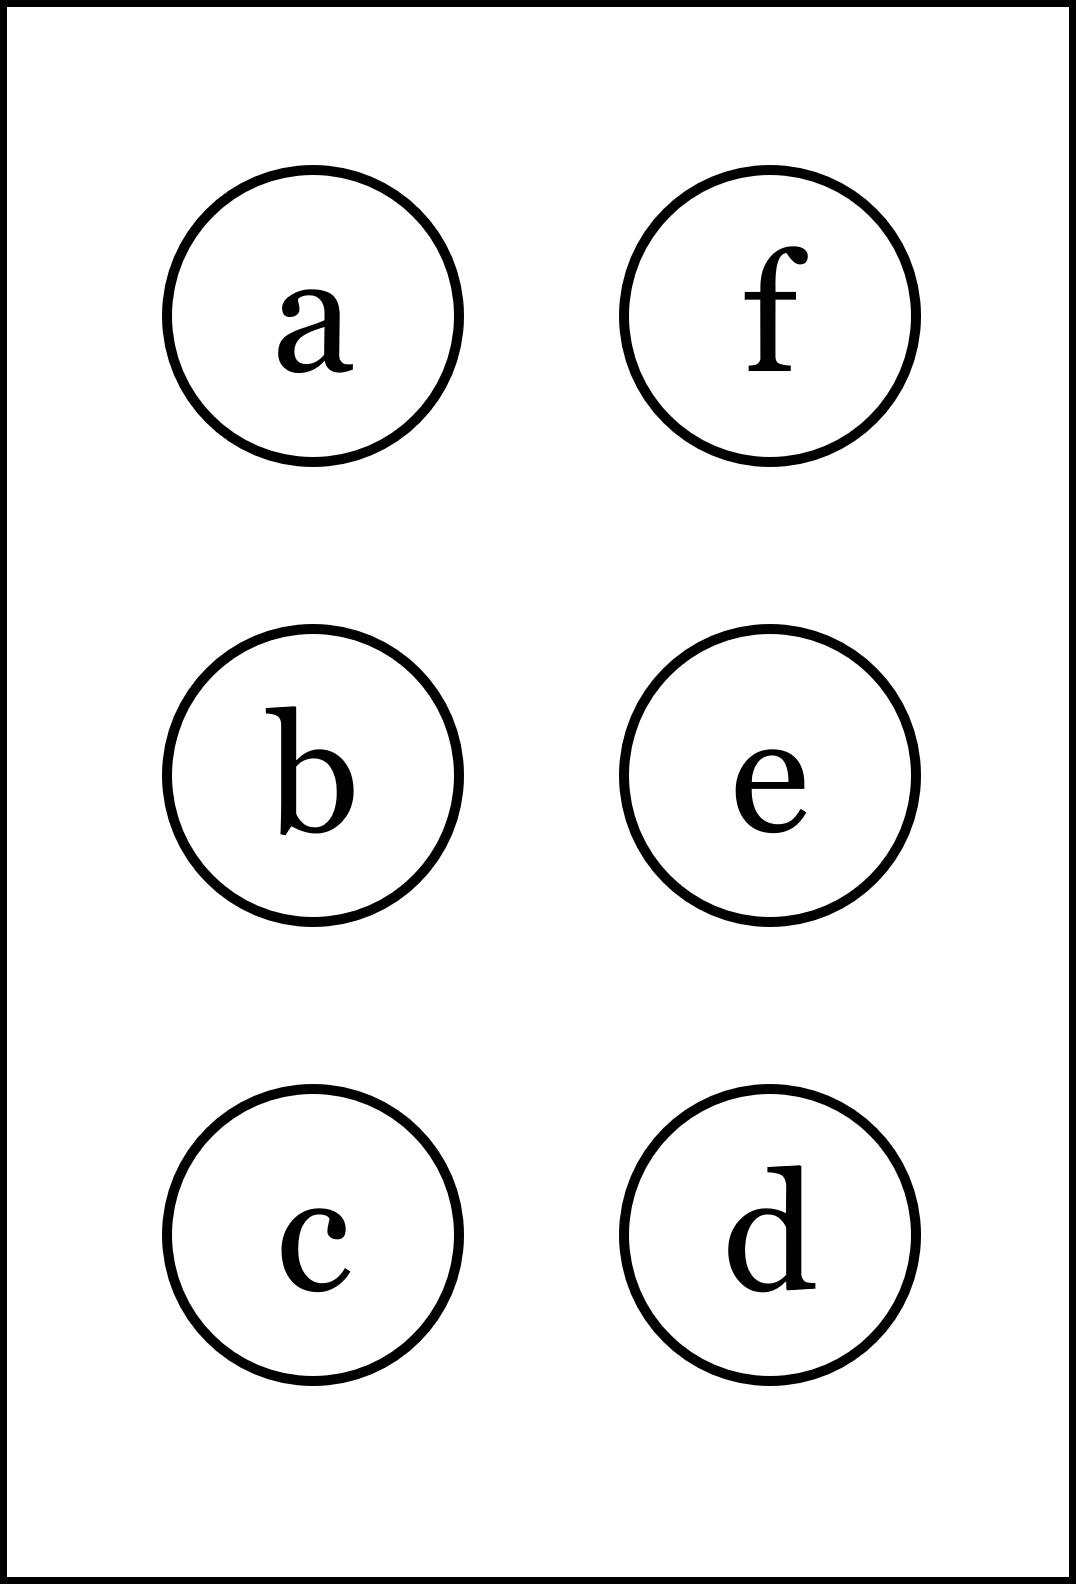
\includegraphics[height=40mm]{../images/braille.png}
{\small Písmeno Braillovej abecedy}
\end{center}
\end{minipage}
\end{center}
\end{minipage}
\\ \hdashline
\begin{minipage}[c][99mm][t]{0.49\linewidth}
\begin{center}
\vspace{7mm}
{\huge Kubická rovnice, skupina \textit{Theta $\theta$} -\romannumeral3}\\[4.5mm]
\textit{Meno:}\phantom{xxxxxxxxxxxxxxxxxxxxxxxxxxxxxxxxxxxxxxxxxxxxxxxxxxxxxxxxxxxxxxxxx}\\[3.5mm]
\textbf{Vypočítej součet kořenů kubické rovnice.} Dvojitý kořen považuj do součtu za dva.\\Analogicky pro trojitý kořen. Pokud ti vyjde stejný výsledek jako je za otazníky, tak\\napravo obarvi příslušející kroužek načerno. \textbf{Spolu odevzdejte výsledné slovo}.\\[3mm]
\begin{minipage}{0.77\linewidth}
\begin{center}
\begin{varwidth}{\textwidth}
\begin{enumerate}
\large
\item $5x^3-20x=0$\quad \dotfill\; ???\;\dotfill \quad 0
\item $2x^3+10x^2-34x-42=0$\quad \dotfill\; ???\;\dotfill \quad 9
\item $-14x^3-53x^2+17x+20=0$\quad \dotfill\; ???\;\dotfill \quad $\nicefrac{-53}{14}$
\item $-18x^3+60x^2-56x+16=0$\quad \dotfill\; ???\;\dotfill \quad 2
\item \quad \dotfill\; ???\;\dotfill \quad vybarvi
\item \quad \dotfill\; ???\;\dotfill \quad vybarvi
\end{enumerate}
\end{varwidth}
\end{center}
\end{minipage}
\begin{minipage}{0.20\linewidth}
\begin{center}
{\Huge\bfseries 3.} \\[2mm]
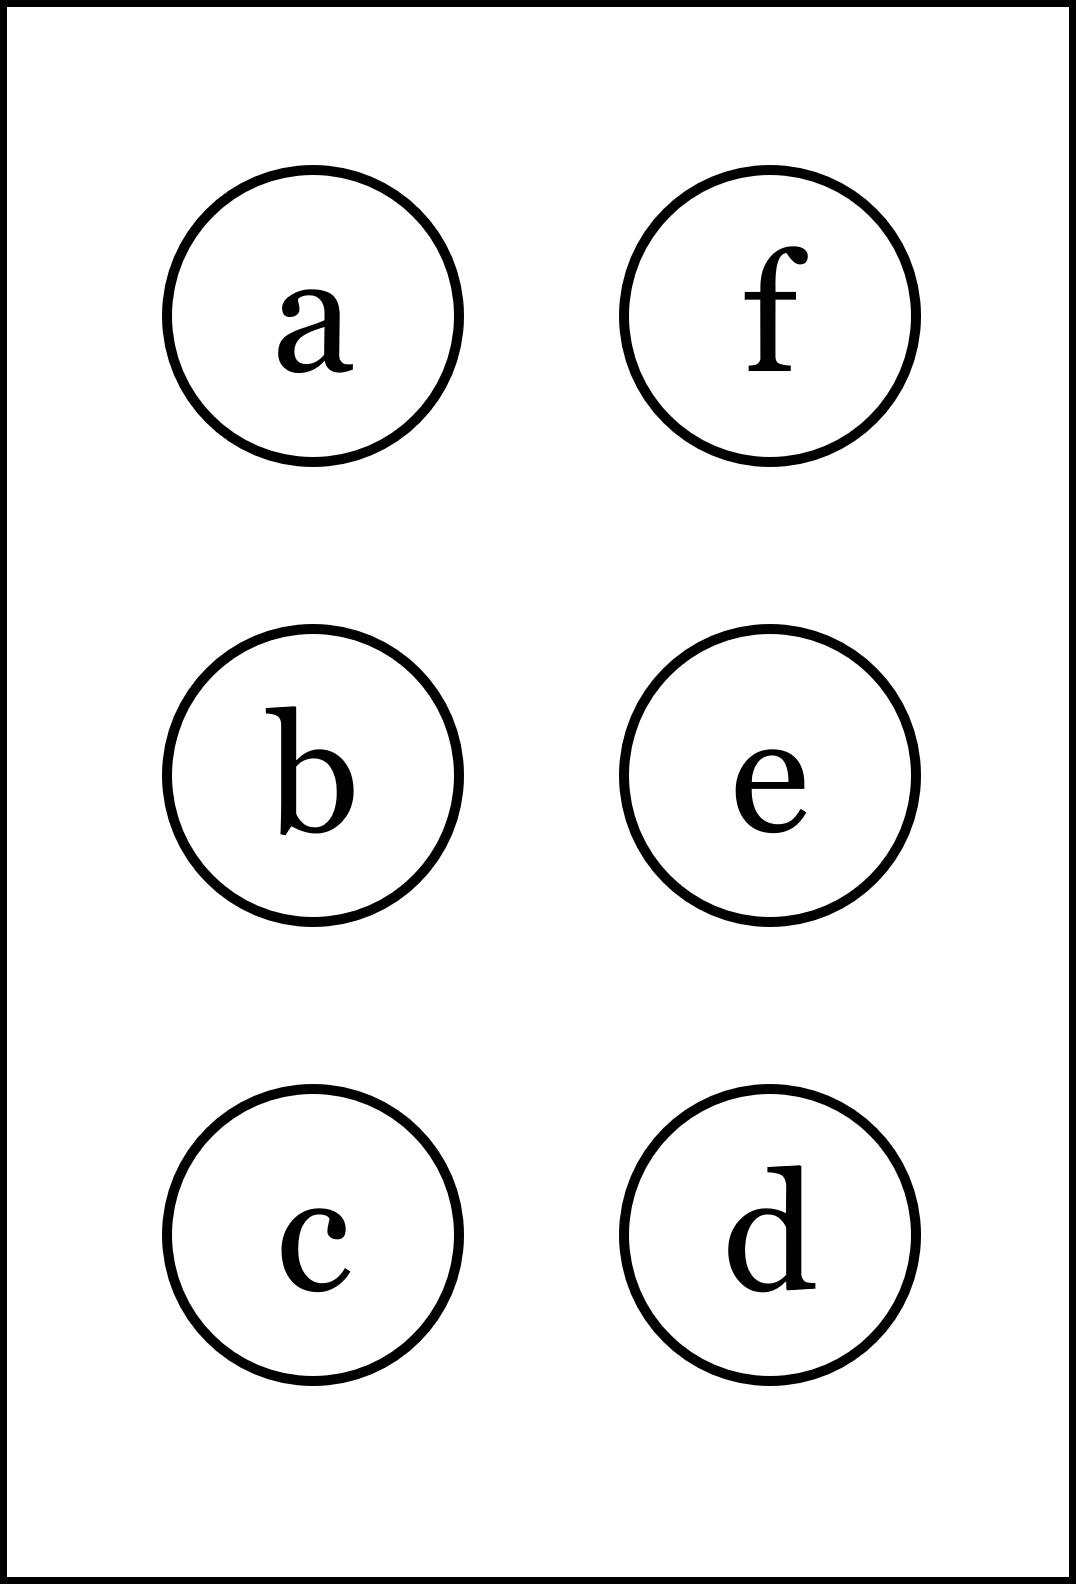
\includegraphics[height=40mm]{../images/braille.png}
{\small Písmeno Braillovej abecedy}
\end{center}
\end{minipage}
\end{center}
\end{minipage}
&
\begin{minipage}[c][99mm][t]{0.49\linewidth}
\begin{center}
\vspace{7mm}
{\huge Kubická rovnice, skupina \textit{Theta $\theta$} -\romannumeral4}\\[4.5mm]
\textit{Meno:}\phantom{xxxxxxxxxxxxxxxxxxxxxxxxxxxxxxxxxxxxxxxxxxxxxxxxxxxxxxxxxxxxxxxxx}\\[3.5mm]
\textbf{Vypočítej součet kořenů kubické rovnice.} Dvojitý kořen považuj do součtu za dva.\\Analogicky pro trojitý kořen. Pokud ti vyjde stejný výsledek jako je za otazníky, tak\\napravo obarvi příslušející kroužek načerno. \textbf{Spolu odevzdejte výsledné slovo}.\\[3mm]
\begin{minipage}{0.77\linewidth}
\begin{center}
\begin{varwidth}{\textwidth}
\begin{enumerate}
\large
\item $-2x^3+8x^2-8x=0$\quad \dotfill\; ???\;\dotfill \quad 4
\item $-3x^3+9x^2+12x-36=0$\quad \dotfill\; ???\;\dotfill \quad 3
\item $-9x^3+63x-54=0$\quad \dotfill\; ???\;\dotfill \quad -6
\item $x^3-13x^2+47x-35=0$\quad \dotfill\; ???\;\dotfill \quad 1
\item \quad \dotfill\; ???\;\dotfill \quad nebarvi
\item \quad \dotfill\; ???\;\dotfill \quad nebarvi
\end{enumerate}
\end{varwidth}
\end{center}
\end{minipage}
\begin{minipage}{0.20\linewidth}
\begin{center}
{\Huge\bfseries 4.} \\[2mm]
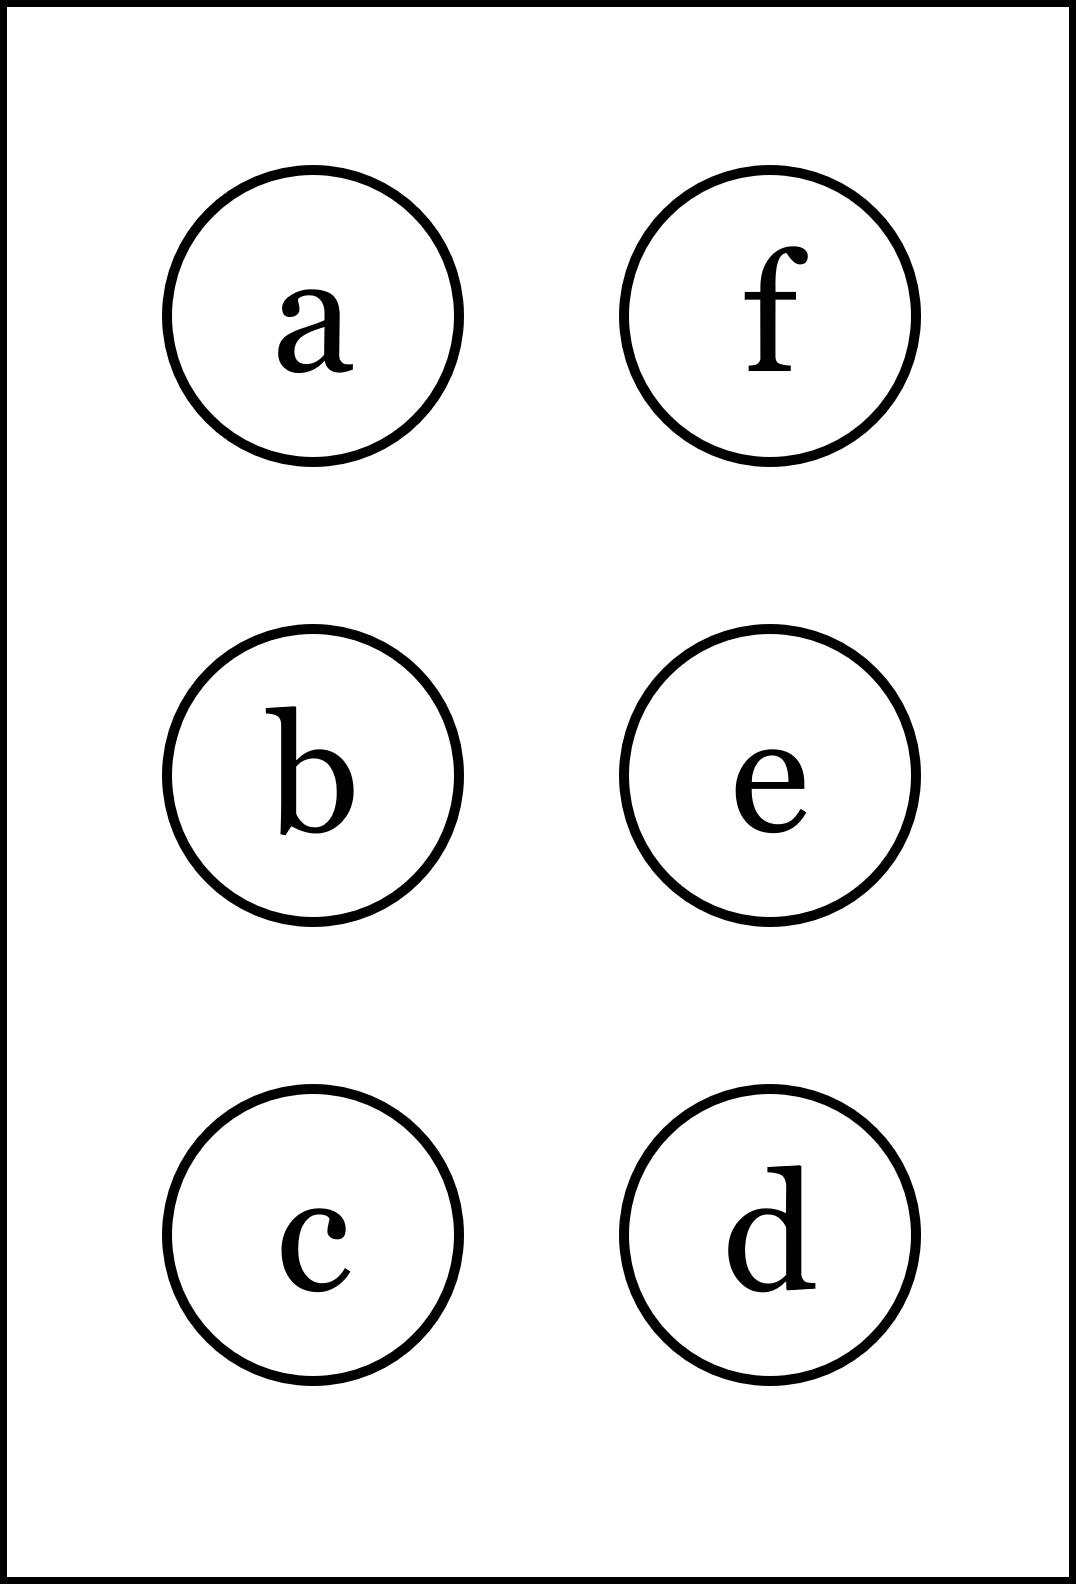
\includegraphics[height=40mm]{../images/braille.png}
{\small Písmeno Braillovej abecedy}
\end{center}
\end{minipage}
\end{center}
\end{minipage}

\end{tabular}
\begin{tikzpicture}[remember picture,overlay]\node[xshift=7mm,yshift=-100.6mm,anchor=north west] at (current page.north west){\ding{33}};\end{tikzpicture}
\begin{tikzpicture}[remember picture,overlay]\node[xshift=151.2mm,yshift=-7mm,anchor=north west,rotate=270] at (current page.north west){\ding{33}};\end{tikzpicture}
\clearpage
\thispagestyle{empty}
\begin{tabular}{c:c}
\begin{minipage}[c][99mm][t]{0.49\linewidth}
\begin{center}
\vspace{7mm}
{\huge Kubická rovnice, skupina \textit{Iota $\iota$} -\romannumeral1}\\[4.5mm]
\textit{Meno:}\phantom{xxxxxxxxxxxxxxxxxxxxxxxxxxxxxxxxxxxxxxxxxxxxxxxxxxxxxxxxxxxxxxxxx}\\[3.5mm]
\textbf{Vypočítej součet kořenů kubické rovnice.} Dvojitý kořen považuj do součtu za dva.\\Analogicky pro trojitý kořen. Pokud ti vyjde stejný výsledek jako je za otazníky, tak\\napravo obarvi příslušející kroužek načerno. \textbf{Spolu odevzdejte výsledné slovo}.\\[3mm]
\begin{minipage}{0.77\linewidth}
\begin{center}
\begin{varwidth}{\textwidth}
\begin{enumerate}
\large
\item $-x^3+9x=0$\quad \dotfill\; ???\;\dotfill \quad -6
\item $-3x^3-12x^2+33x-18=0$\quad \dotfill\; ???\;\dotfill \quad -4
\item $3x^3+10x^2-44x+24=0$\quad \dotfill\; ???\;\dotfill \quad $\nicefrac{14}{3}$
\item $4x^3-2x^2-24x-18=0$\quad \dotfill\; ???\;\dotfill \quad $\nicefrac{-5}{2}$
\item \quad \dotfill\; ???\;\dotfill \quad nebarvi
\item \quad \dotfill\; ???\;\dotfill \quad vybarvi
\end{enumerate}
\end{varwidth}
\end{center}
\end{minipage}
\begin{minipage}{0.20\linewidth}
\begin{center}
{\Huge\bfseries 1.} \\[2mm]
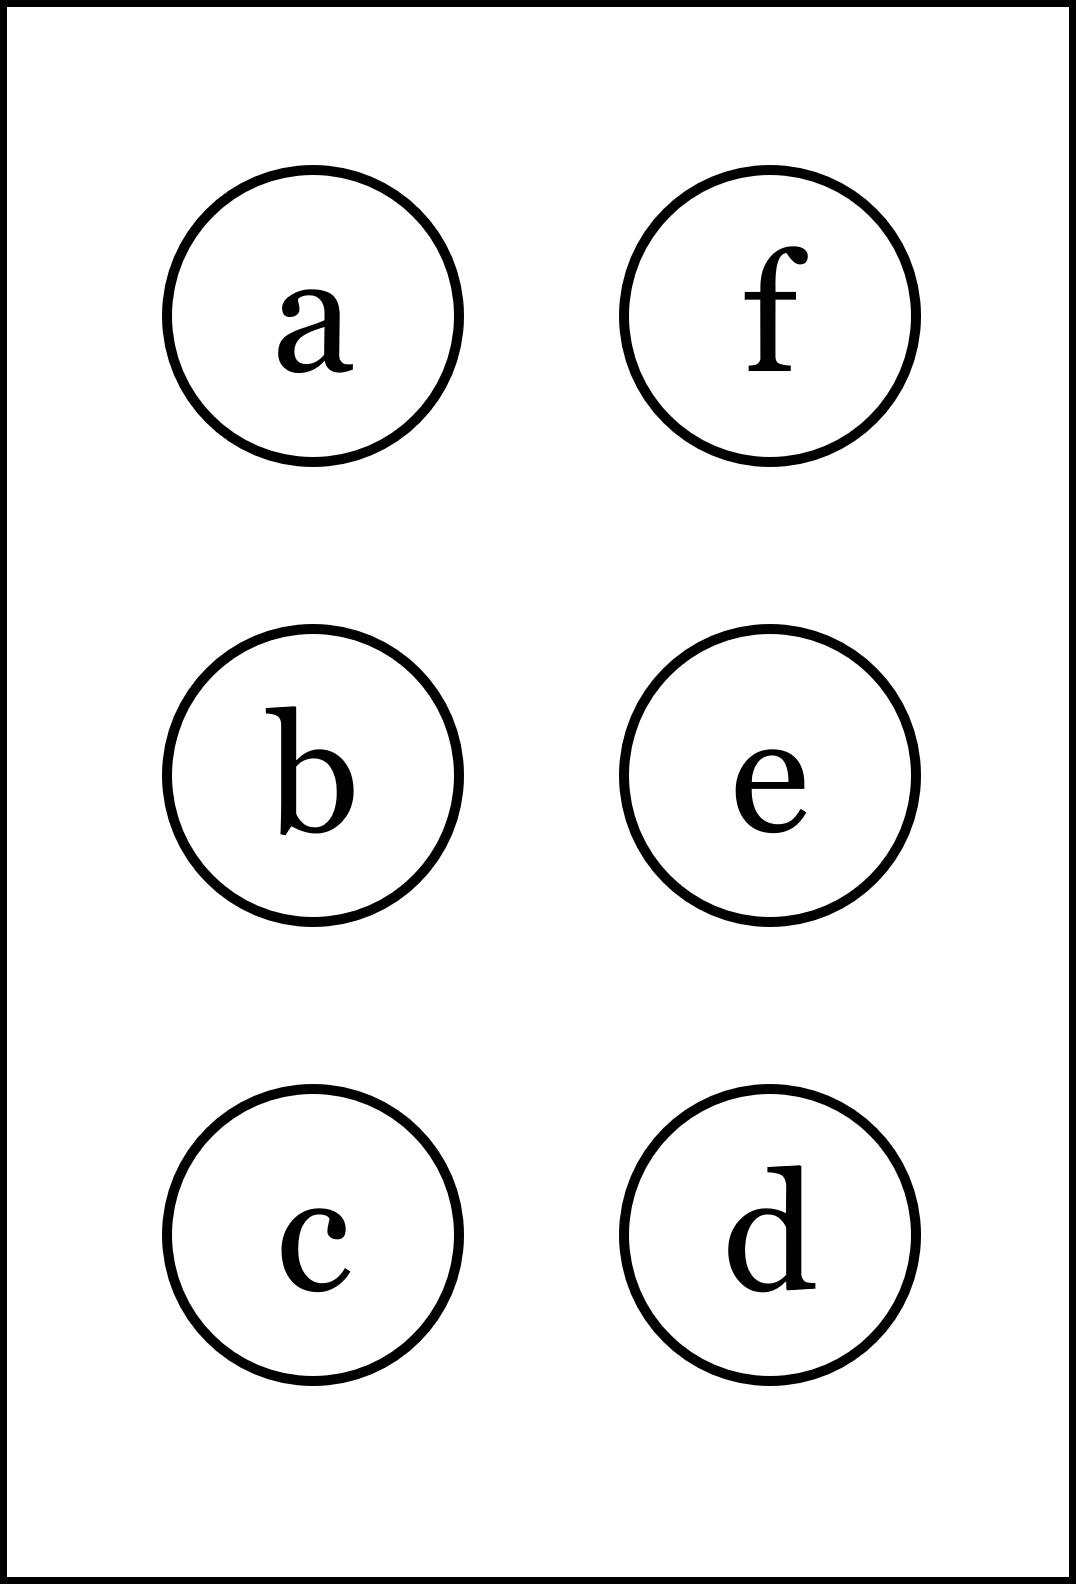
\includegraphics[height=40mm]{../images/braille.png}
{\small Písmeno Braillovej abecedy}
\end{center}
\end{minipage}
\end{center}
\end{minipage}
&
\begin{minipage}[c][99mm][t]{0.49\linewidth}
\begin{center}
\vspace{7mm}
{\huge Kubická rovnice, skupina \textit{Iota $\iota$} -\romannumeral2}\\[4.5mm]
\textit{Meno:}\phantom{xxxxxxxxxxxxxxxxxxxxxxxxxxxxxxxxxxxxxxxxxxxxxxxxxxxxxxxxxxxxxxxxx}\\[3.5mm]
\textbf{Vypočítej součet kořenů kubické rovnice.} Dvojitý kořen považuj do součtu za dva.\\Analogicky pro trojitý kořen. Pokud ti vyjde stejný výsledek jako je za otazníky, tak\\napravo obarvi příslušející kroužek načerno. \textbf{Spolu odevzdejte výsledné slovo}.\\[3mm]
\begin{minipage}{0.77\linewidth}
\begin{center}
\begin{varwidth}{\textwidth}
\begin{enumerate}
\large
\item $4x^3-32x^2-36x=0$\quad \dotfill\; ???\;\dotfill \quad 8
\item $3x^3-15x^2+9x+27=0$\quad \dotfill\; ???\;\dotfill \quad 5
\item $12x^3-9x-3=0$\quad \dotfill\; ???\;\dotfill \quad 1
\item $6x^3-20x^2+18x-4=0$\quad \dotfill\; ???\;\dotfill \quad $\nicefrac{-8}{3}$
\item \quad \dotfill\; ???\;\dotfill \quad vybarvi
\item \quad \dotfill\; ???\;\dotfill \quad vybarvi
\end{enumerate}
\end{varwidth}
\end{center}
\end{minipage}
\begin{minipage}{0.20\linewidth}
\begin{center}
{\Huge\bfseries 2.} \\[2mm]
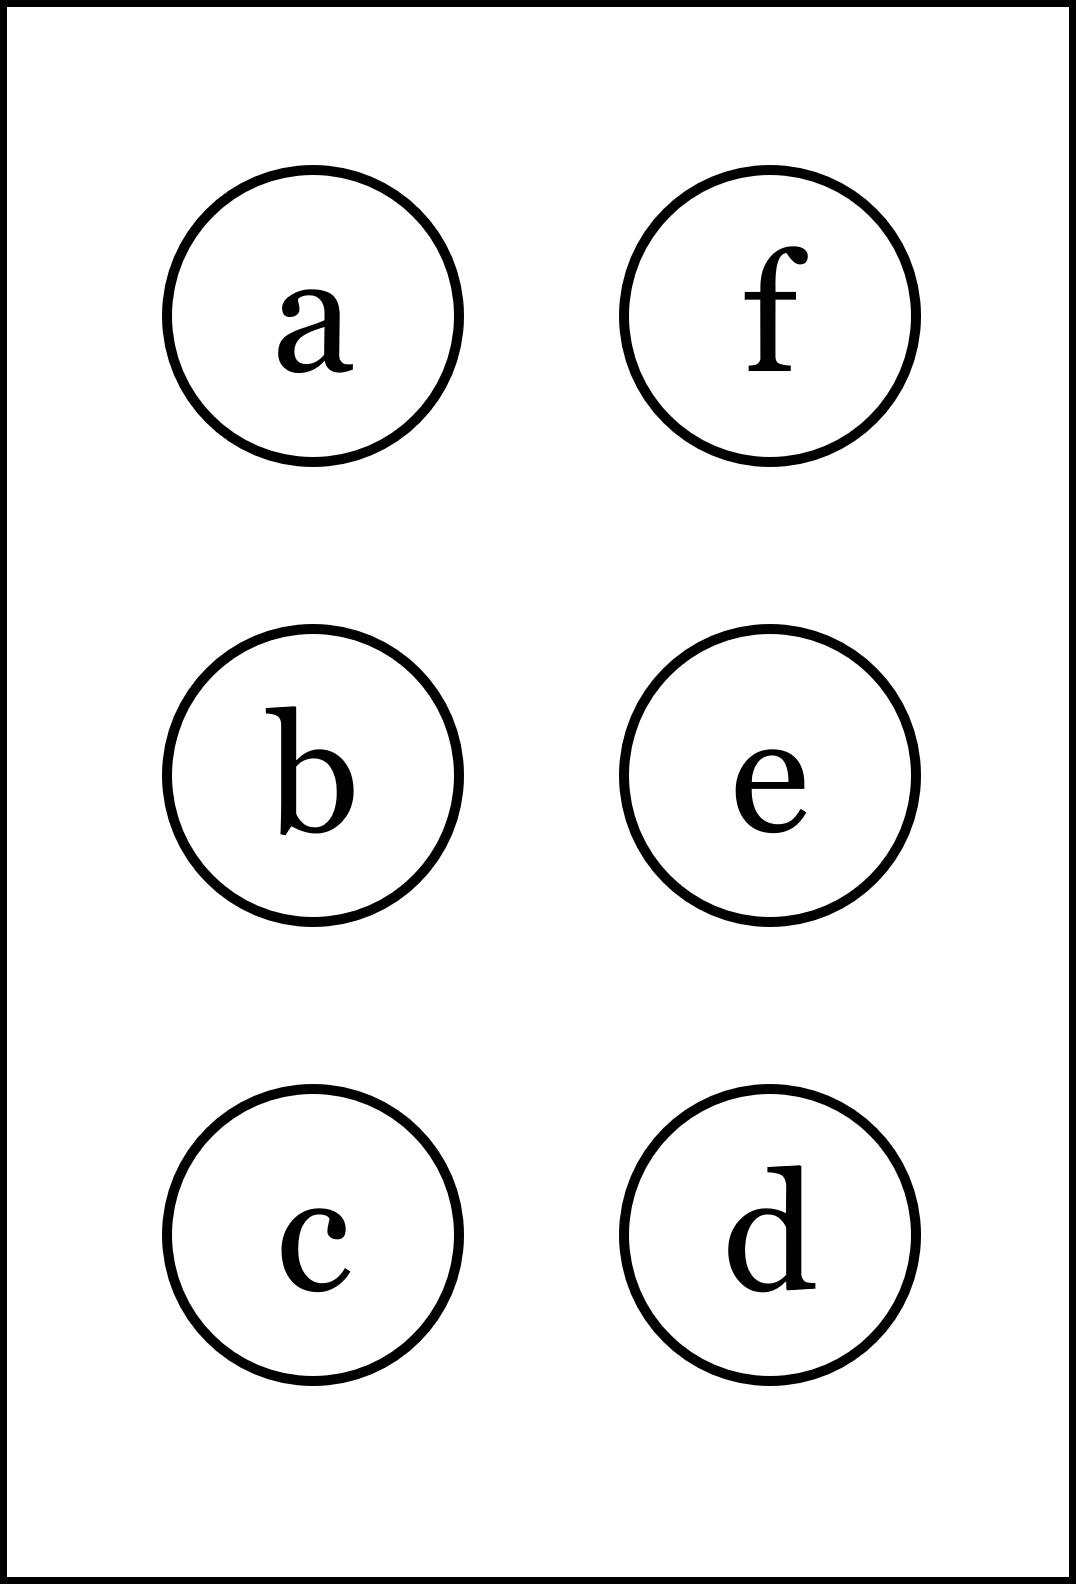
\includegraphics[height=40mm]{../images/braille.png}
{\small Písmeno Braillovej abecedy}
\end{center}
\end{minipage}
\end{center}
\end{minipage}
\\ \hdashline
\begin{minipage}[c][99mm][t]{0.49\linewidth}
\begin{center}
\vspace{7mm}
{\huge Kubická rovnice, skupina \textit{Iota $\iota$} -\romannumeral3}\\[4.5mm]
\textit{Meno:}\phantom{xxxxxxxxxxxxxxxxxxxxxxxxxxxxxxxxxxxxxxxxxxxxxxxxxxxxxxxxxxxxxxxxx}\\[3.5mm]
\textbf{Vypočítej součet kořenů kubické rovnice.} Dvojitý kořen považuj do součtu za dva.\\Analogicky pro trojitý kořen. Pokud ti vyjde stejný výsledek jako je za otazníky, tak\\napravo obarvi příslušející kroužek načerno. \textbf{Spolu odevzdejte výsledné slovo}.\\[3mm]
\begin{minipage}{0.77\linewidth}
\begin{center}
\begin{varwidth}{\textwidth}
\begin{enumerate}
\large
\item $-x^3-7x^2+8x=0$\quad \dotfill\; ???\;\dotfill \quad -7
\item $3x^3-12x^2-21x+30=0$\quad \dotfill\; ???\;\dotfill \quad 4
\item $-8x^3-48x^2-88x-48=0$\quad \dotfill\; ???\;\dotfill \quad -6
\item $-6x^3-7x^2+11x+12=0$\quad \dotfill\; ???\;\dotfill \quad $\nicefrac{11}{6}$
\item \quad \dotfill\; ???\;\dotfill \quad nebarvi
\item \quad \dotfill\; ???\;\dotfill \quad nebarvi
\end{enumerate}
\end{varwidth}
\end{center}
\end{minipage}
\begin{minipage}{0.20\linewidth}
\begin{center}
{\Huge\bfseries 3.} \\[2mm]
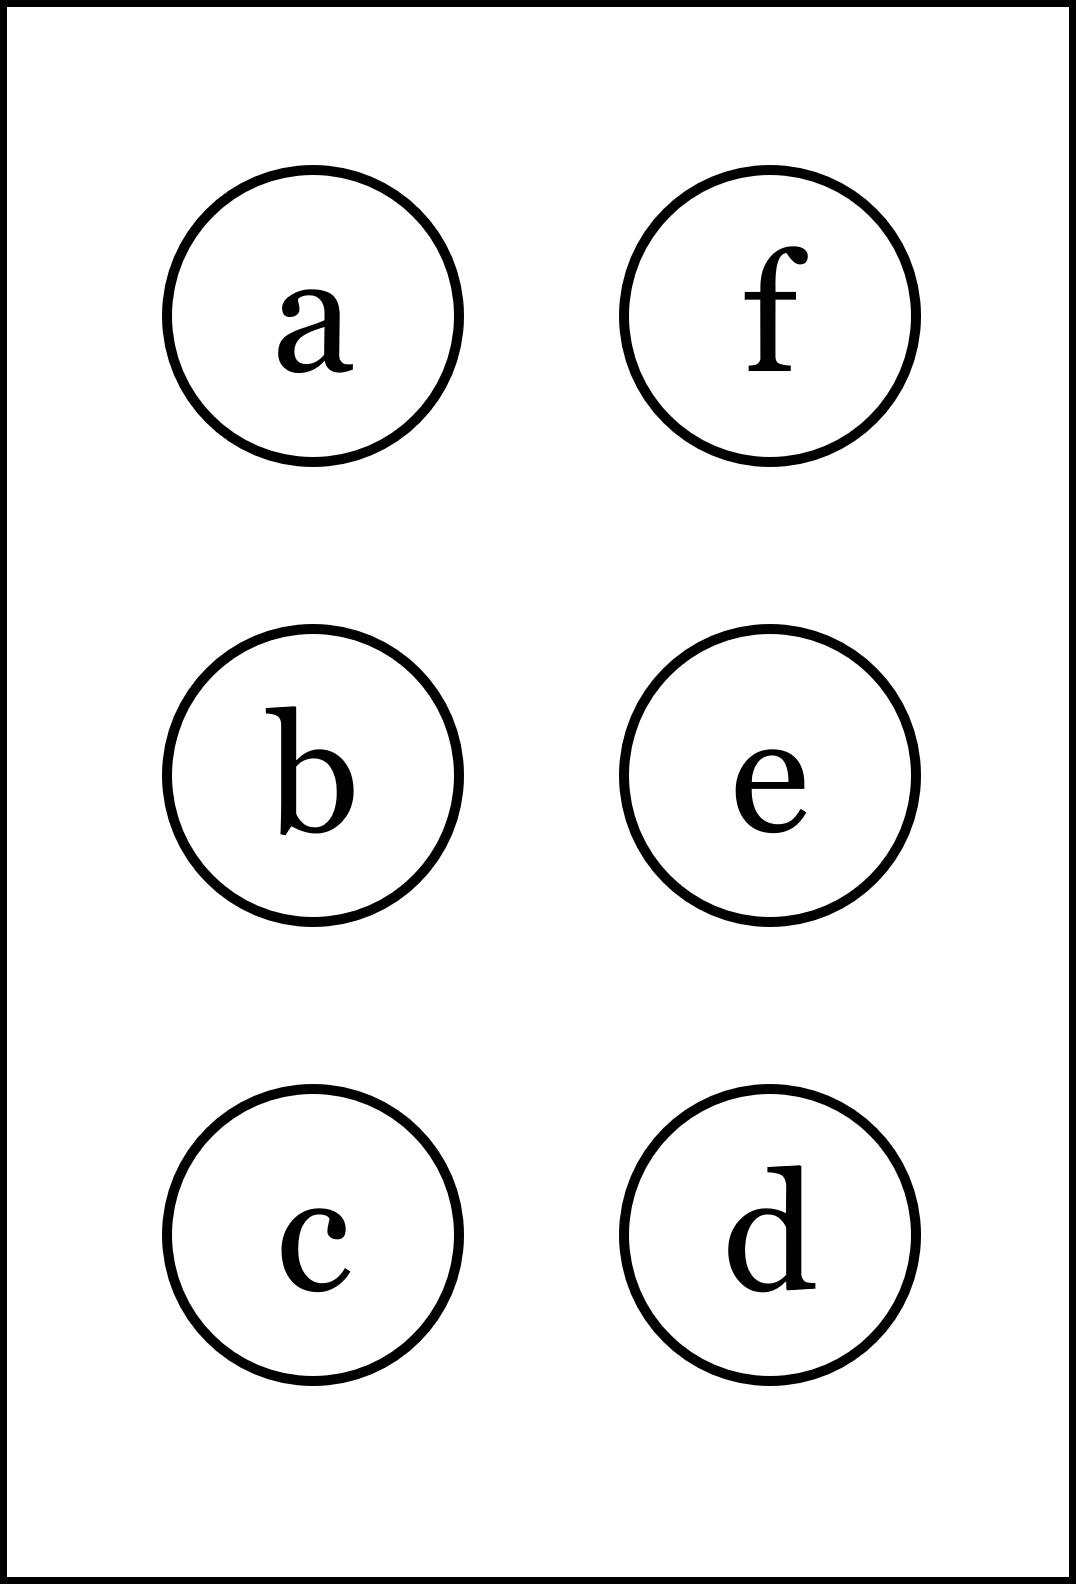
\includegraphics[height=40mm]{../images/braille.png}
{\small Písmeno Braillovej abecedy}
\end{center}
\end{minipage}
\end{center}
\end{minipage}
&
\begin{minipage}[c][99mm][t]{0.49\linewidth}
\begin{center}
\vspace{7mm}
{\huge Kubická rovnice, skupina \textit{Iota $\iota$} -\romannumeral4}\\[4.5mm]
\textit{Meno:}\phantom{xxxxxxxxxxxxxxxxxxxxxxxxxxxxxxxxxxxxxxxxxxxxxxxxxxxxxxxxxxxxxxxxx}\\[3.5mm]
\textbf{Vypočítej součet kořenů kubické rovnice.} Dvojitý kořen považuj do součtu za dva.\\Analogicky pro trojitý kořen. Pokud ti vyjde stejný výsledek jako je za otazníky, tak\\napravo obarvi příslušející kroužek načerno. \textbf{Spolu odevzdejte výsledné slovo}.\\[3mm]
\begin{minipage}{0.77\linewidth}
\begin{center}
\begin{varwidth}{\textwidth}
\begin{enumerate}
\large
\item $x^3-3x^2-18x=0$\quad \dotfill\; ???\;\dotfill \quad 3
\item $-2x^3-2x^2+10x-6=0$\quad \dotfill\; ???\;\dotfill \quad -3
\item $-12x^3+38x^2-4x-6=0$\quad \dotfill\; ???\;\dotfill \quad $\nicefrac{19}{6}$
\item $42x^3+55x^2+14x+1=0$\quad \dotfill\; ???\;\dotfill \quad $\nicefrac{-55}{42}$
\item \quad \dotfill\; ???\;\dotfill \quad nebarvi
\item \quad \dotfill\; ???\;\dotfill \quad nebarvi
\end{enumerate}
\end{varwidth}
\end{center}
\end{minipage}
\begin{minipage}{0.20\linewidth}
\begin{center}
{\Huge\bfseries 4.} \\[2mm]
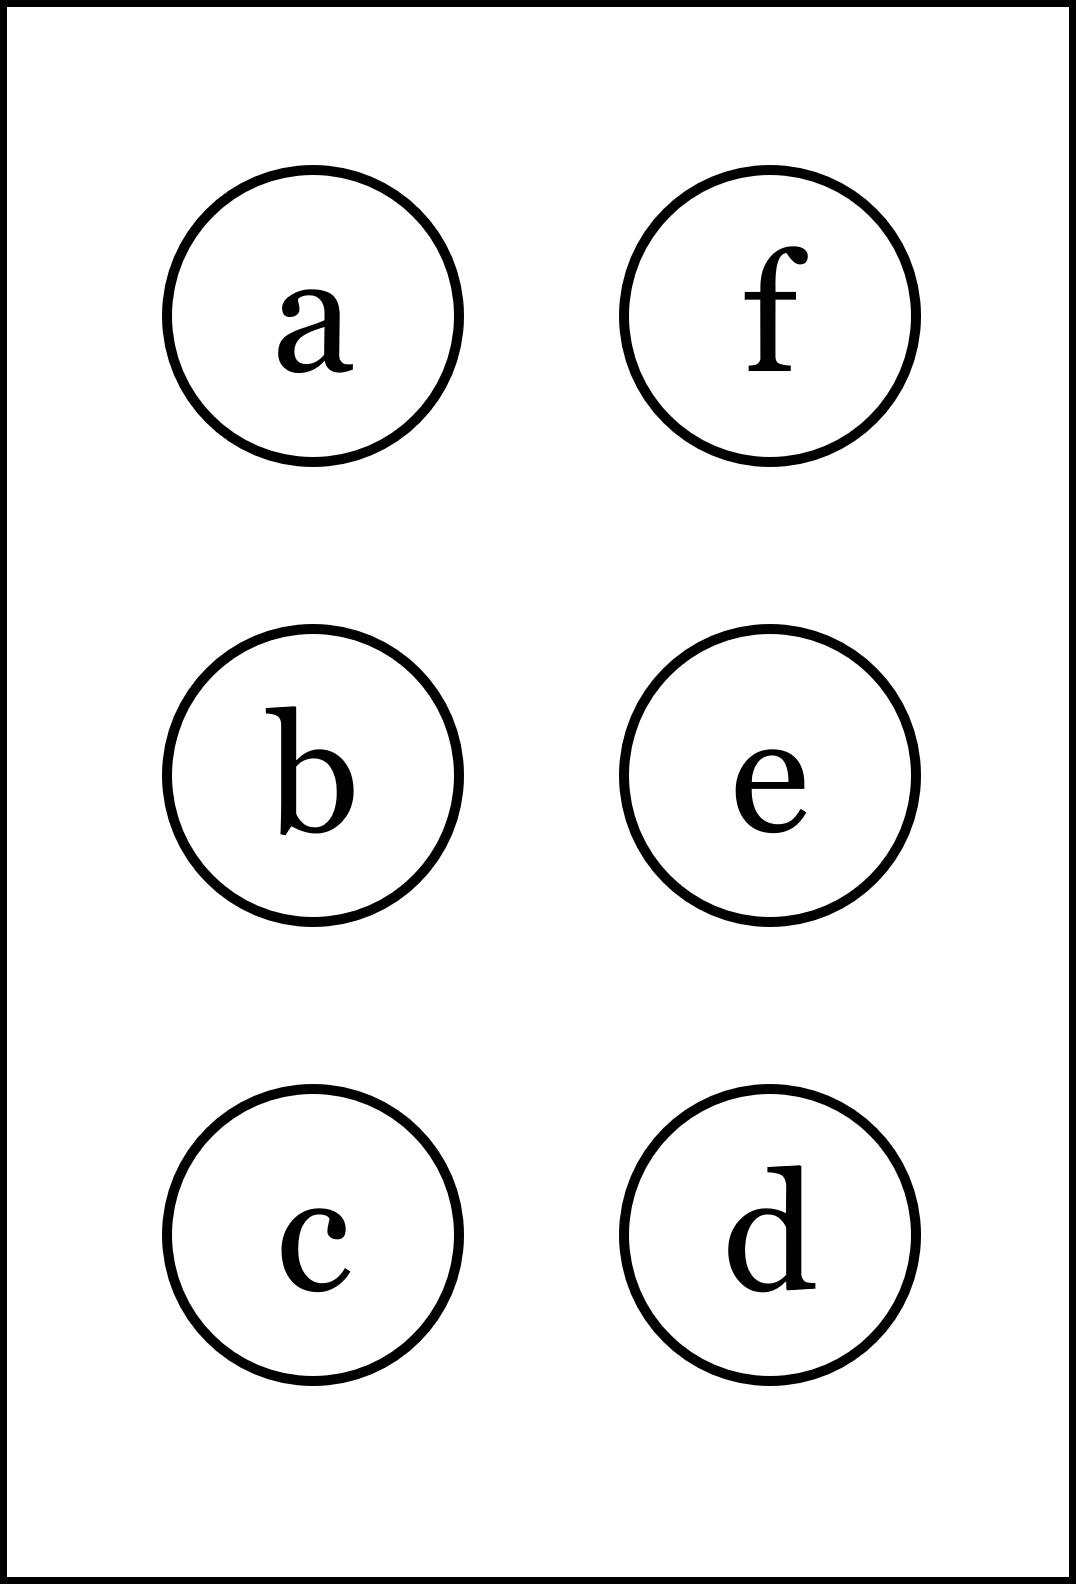
\includegraphics[height=40mm]{../images/braille.png}
{\small Písmeno Braillovej abecedy}
\end{center}
\end{minipage}
\end{center}
\end{minipage}

\end{tabular}
\begin{tikzpicture}[remember picture,overlay]\node[xshift=7mm,yshift=-100.6mm,anchor=north west] at (current page.north west){\ding{33}};\end{tikzpicture}
\begin{tikzpicture}[remember picture,overlay]\node[xshift=151.2mm,yshift=-7mm,anchor=north west,rotate=270] at (current page.north west){\ding{33}};\end{tikzpicture}
\clearpage
\thispagestyle{empty}
\begin{tabular}{c:c}
\begin{minipage}[c][99mm][t]{0.49\linewidth}
\begin{center}
\vspace{7mm}
{\huge Kubická rovnice, skupina \textit{Kappa $\kappa$} -\romannumeral1}\\[4.5mm]
\textit{Meno:}\phantom{xxxxxxxxxxxxxxxxxxxxxxxxxxxxxxxxxxxxxxxxxxxxxxxxxxxxxxxxxxxxxxxxx}\\[3.5mm]
\textbf{Vypočítej součet kořenů kubické rovnice.} Dvojitý kořen považuj do součtu za dva.\\Analogicky pro trojitý kořen. Pokud ti vyjde stejný výsledek jako je za otazníky, tak\\napravo obarvi příslušející kroužek načerno. \textbf{Spolu odevzdejte výsledné slovo}.\\[3mm]
\begin{minipage}{0.77\linewidth}
\begin{center}
\begin{varwidth}{\textwidth}
\begin{enumerate}
\large
\item $-x^3+6x^2-5x=0$\quad \dotfill\; ???\;\dotfill \quad 6
\item $x^3-4x^2-11x-6=0$\quad \dotfill\; ???\;\dotfill \quad 4
\item $-16x^3+28x^2+56x+12=0$\quad \dotfill\; ???\;\dotfill \quad $\nicefrac{15}{4}$
\item $9x^3-6x^2-20x-8=0$\quad \dotfill\; ???\;\dotfill \quad 2
\item \quad \dotfill\; ???\;\dotfill \quad vybarvi
\item \quad \dotfill\; ???\;\dotfill \quad nebarvi
\end{enumerate}
\end{varwidth}
\end{center}
\end{minipage}
\begin{minipage}{0.20\linewidth}
\begin{center}
{\Huge\bfseries 1.} \\[2mm]
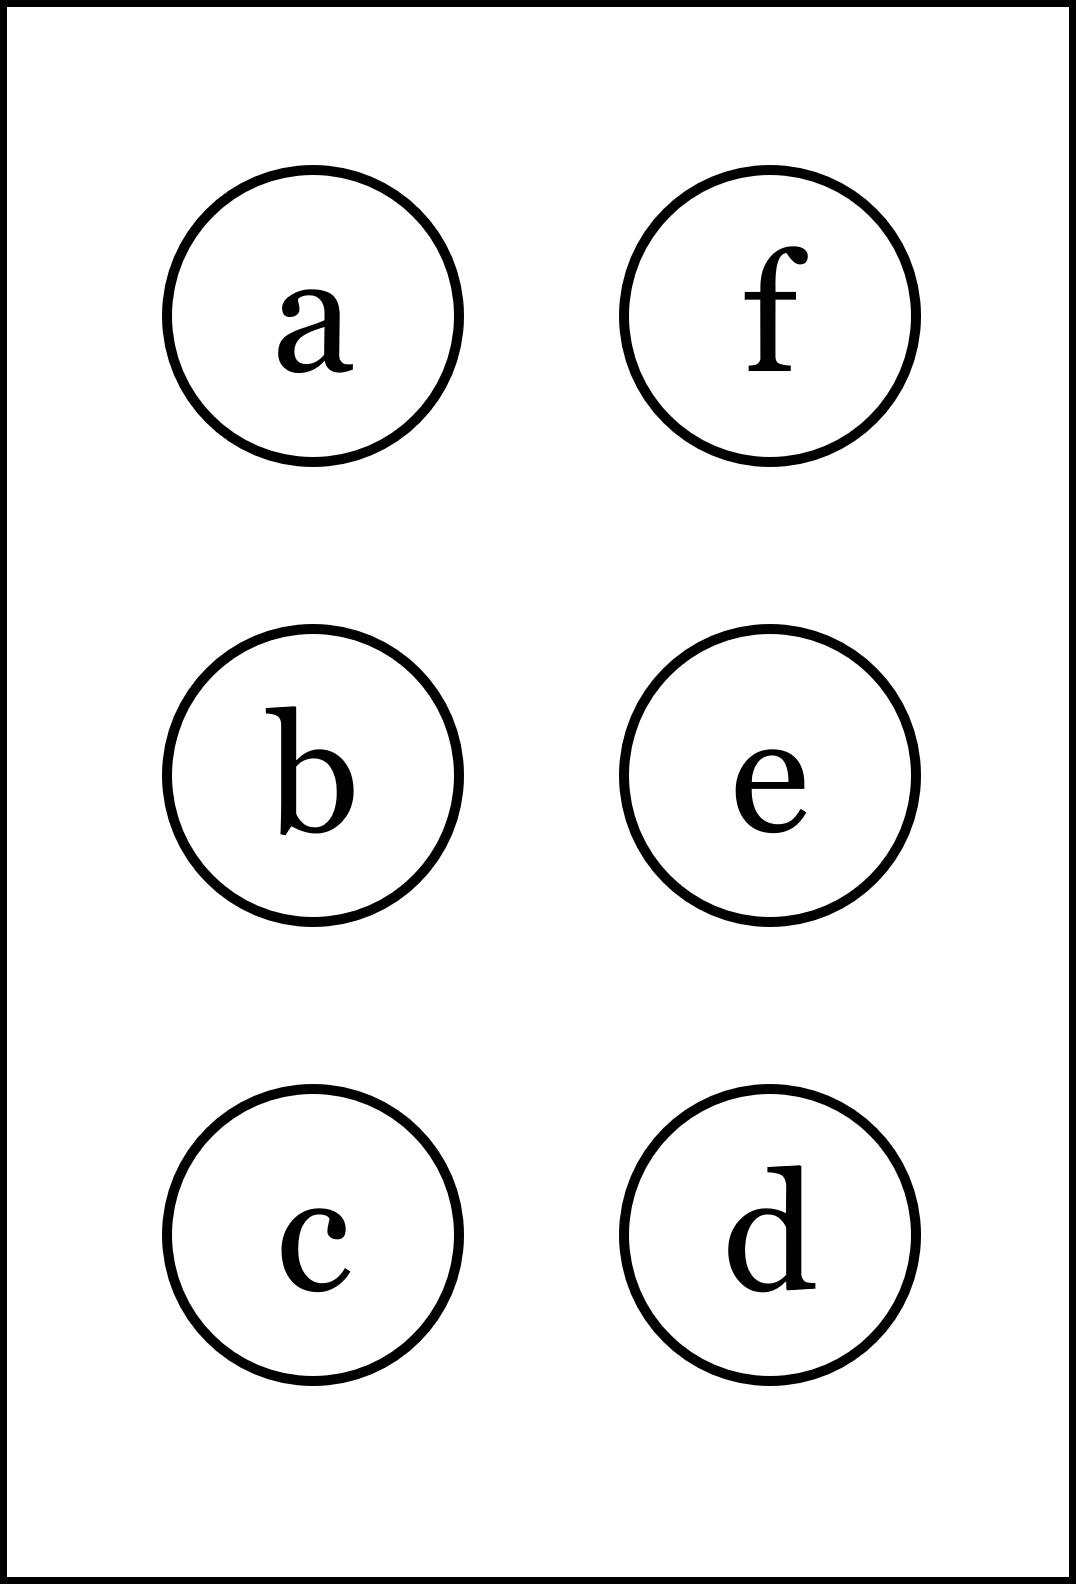
\includegraphics[height=40mm]{../images/braille.png}
{\small Písmeno Braillovej abecedy}
\end{center}
\end{minipage}
\end{center}
\end{minipage}
&
\begin{minipage}[c][99mm][t]{0.49\linewidth}
\begin{center}
\vspace{7mm}
{\huge Kubická rovnice, skupina \textit{Kappa $\kappa$} -\romannumeral2}\\[4.5mm]
\textit{Meno:}\phantom{xxxxxxxxxxxxxxxxxxxxxxxxxxxxxxxxxxxxxxxxxxxxxxxxxxxxxxxxxxxxxxxxx}\\[3.5mm]
\textbf{Vypočítej součet kořenů kubické rovnice.} Dvojitý kořen považuj do součtu za dva.\\Analogicky pro trojitý kořen. Pokud ti vyjde stejný výsledek jako je za otazníky, tak\\napravo obarvi příslušející kroužek načerno. \textbf{Spolu odevzdejte výsledné slovo}.\\[3mm]
\begin{minipage}{0.77\linewidth}
\begin{center}
\begin{varwidth}{\textwidth}
\begin{enumerate}
\large
\item $-x^3+3x^2-2x=0$\quad \dotfill\; ???\;\dotfill \quad 3
\item $7x^3+35x^2-7x-35=0$\quad \dotfill\; ???\;\dotfill \quad -5
\item $-6x^3+21x^2-12x-12=0$\quad \dotfill\; ???\;\dotfill \quad $\nicefrac{7}{2}$
\item $8x^3-10x^2+x+1=0$\quad \dotfill\; ???\;\dotfill \quad $\nicefrac{1}{4}$
\item \quad \dotfill\; ???\;\dotfill \quad nebarvi
\item \quad \dotfill\; ???\;\dotfill \quad nebarvi
\end{enumerate}
\end{varwidth}
\end{center}
\end{minipage}
\begin{minipage}{0.20\linewidth}
\begin{center}
{\Huge\bfseries 2.} \\[2mm]
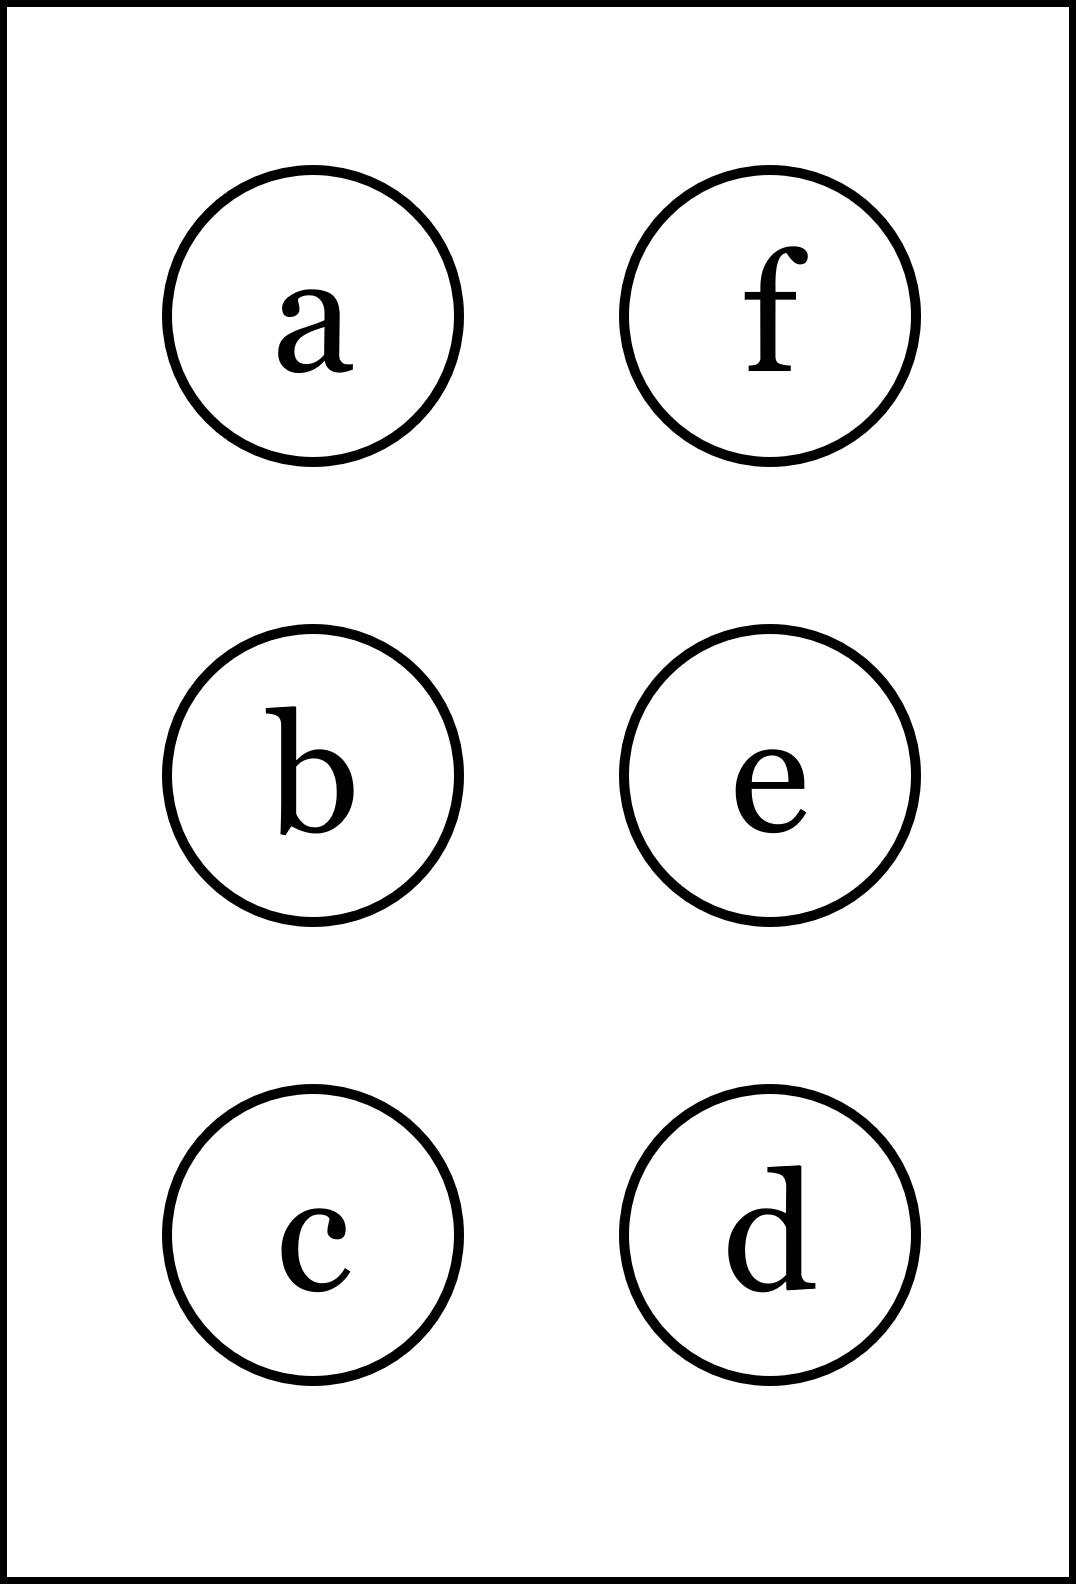
\includegraphics[height=40mm]{../images/braille.png}
{\small Písmeno Braillovej abecedy}
\end{center}
\end{minipage}
\end{center}
\end{minipage}
\\ \hdashline
\begin{minipage}[c][99mm][t]{0.49\linewidth}
\begin{center}
\vspace{7mm}
{\huge Kubická rovnice, skupina \textit{Kappa $\kappa$} -\romannumeral3}\\[4.5mm]
\textit{Meno:}\phantom{xxxxxxxxxxxxxxxxxxxxxxxxxxxxxxxxxxxxxxxxxxxxxxxxxxxxxxxxxxxxxxxxx}\\[3.5mm]
\textbf{Vypočítej součet kořenů kubické rovnice.} Dvojitý kořen považuj do součtu za dva.\\Analogicky pro trojitý kořen. Pokud ti vyjde stejný výsledek jako je za otazníky, tak\\napravo obarvi příslušející kroužek načerno. \textbf{Spolu odevzdejte výsledné slovo}.\\[3mm]
\begin{minipage}{0.77\linewidth}
\begin{center}
\begin{varwidth}{\textwidth}
\begin{enumerate}
\large
\item $-4x^3+16x=0$\quad \dotfill\; ???\;\dotfill \quad 0
\item $x^3-12x^2+47x-60=0$\quad \dotfill\; ???\;\dotfill \quad -4
\item $-4x^3+12x^2-9x+2=0$\quad \dotfill\; ???\;\dotfill \quad -2
\item $-15x^3+28x^2+47x+12=0$\quad \dotfill\; ???\;\dotfill \quad $\nicefrac{38}{15}$
\item \quad \dotfill\; ???\;\dotfill \quad nebarvi
\item \quad \dotfill\; ???\;\dotfill \quad nebarvi
\end{enumerate}
\end{varwidth}
\end{center}
\end{minipage}
\begin{minipage}{0.20\linewidth}
\begin{center}
{\Huge\bfseries 3.} \\[2mm]
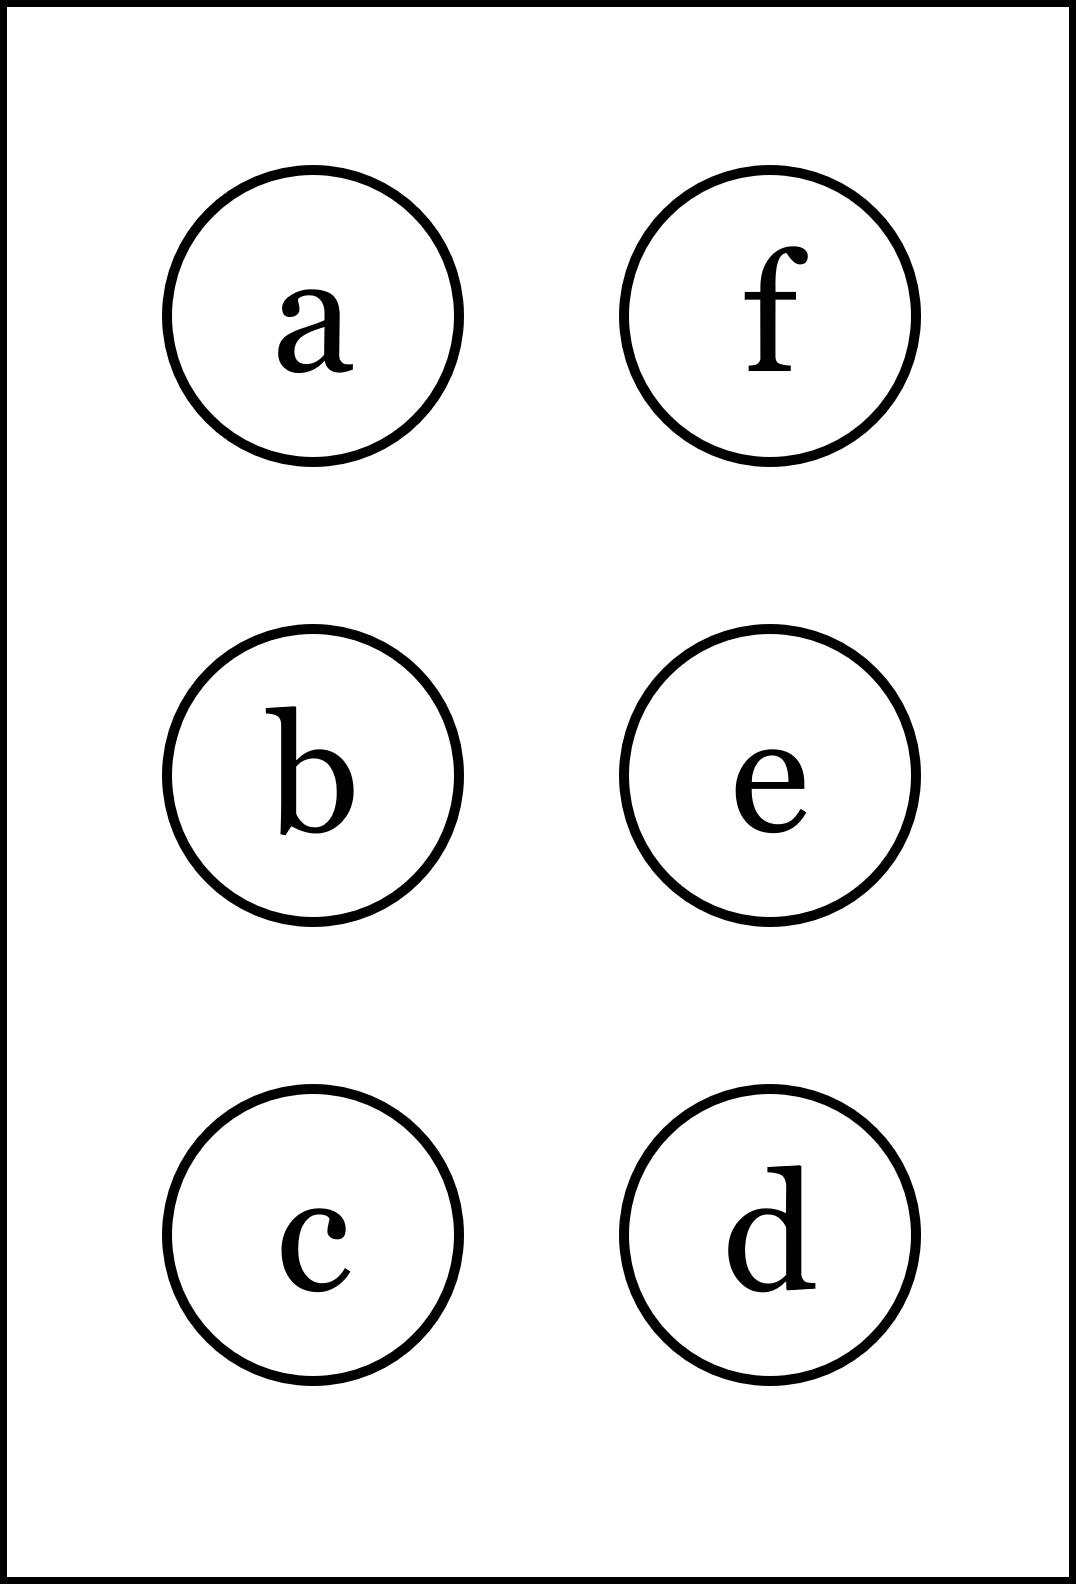
\includegraphics[height=40mm]{../images/braille.png}
{\small Písmeno Braillovej abecedy}
\end{center}
\end{minipage}
\end{center}
\end{minipage}
&
\begin{minipage}[c][99mm][t]{0.49\linewidth}
\begin{center}
\vspace{7mm}
{\huge Kubická rovnice, skupina \textit{Kappa $\kappa$} -\romannumeral4}\\[4.5mm]
\textit{Meno:}\phantom{xxxxxxxxxxxxxxxxxxxxxxxxxxxxxxxxxxxxxxxxxxxxxxxxxxxxxxxxxxxxxxxxx}\\[3.5mm]
\textbf{Vypočítej součet kořenů kubické rovnice.} Dvojitý kořen považuj do součtu za dva.\\Analogicky pro trojitý kořen. Pokud ti vyjde stejný výsledek jako je za otazníky, tak\\napravo obarvi příslušející kroužek načerno. \textbf{Spolu odevzdejte výsledné slovo}.\\[3mm]
\begin{minipage}{0.77\linewidth}
\begin{center}
\begin{varwidth}{\textwidth}
\begin{enumerate}
\large
\item $x^3-4x^2-5x=0$\quad \dotfill\; ???\;\dotfill \quad 4
\item $-x^3+4x^2+29x+24=0$\quad \dotfill\; ???\;\dotfill \quad -12
\item $-32x^3-32x^2+40x+24=0$\quad \dotfill\; ???\;\dotfill \quad 0
\item $-12x^3-49x^2-43x+14=0$\quad \dotfill\; ???\;\dotfill \quad $\nicefrac{7}{12}$
\item \quad \dotfill\; ???\;\dotfill \quad vybarvi
\item \quad \dotfill\; ???\;\dotfill \quad vybarvi
\end{enumerate}
\end{varwidth}
\end{center}
\end{minipage}
\begin{minipage}{0.20\linewidth}
\begin{center}
{\Huge\bfseries 4.} \\[2mm]
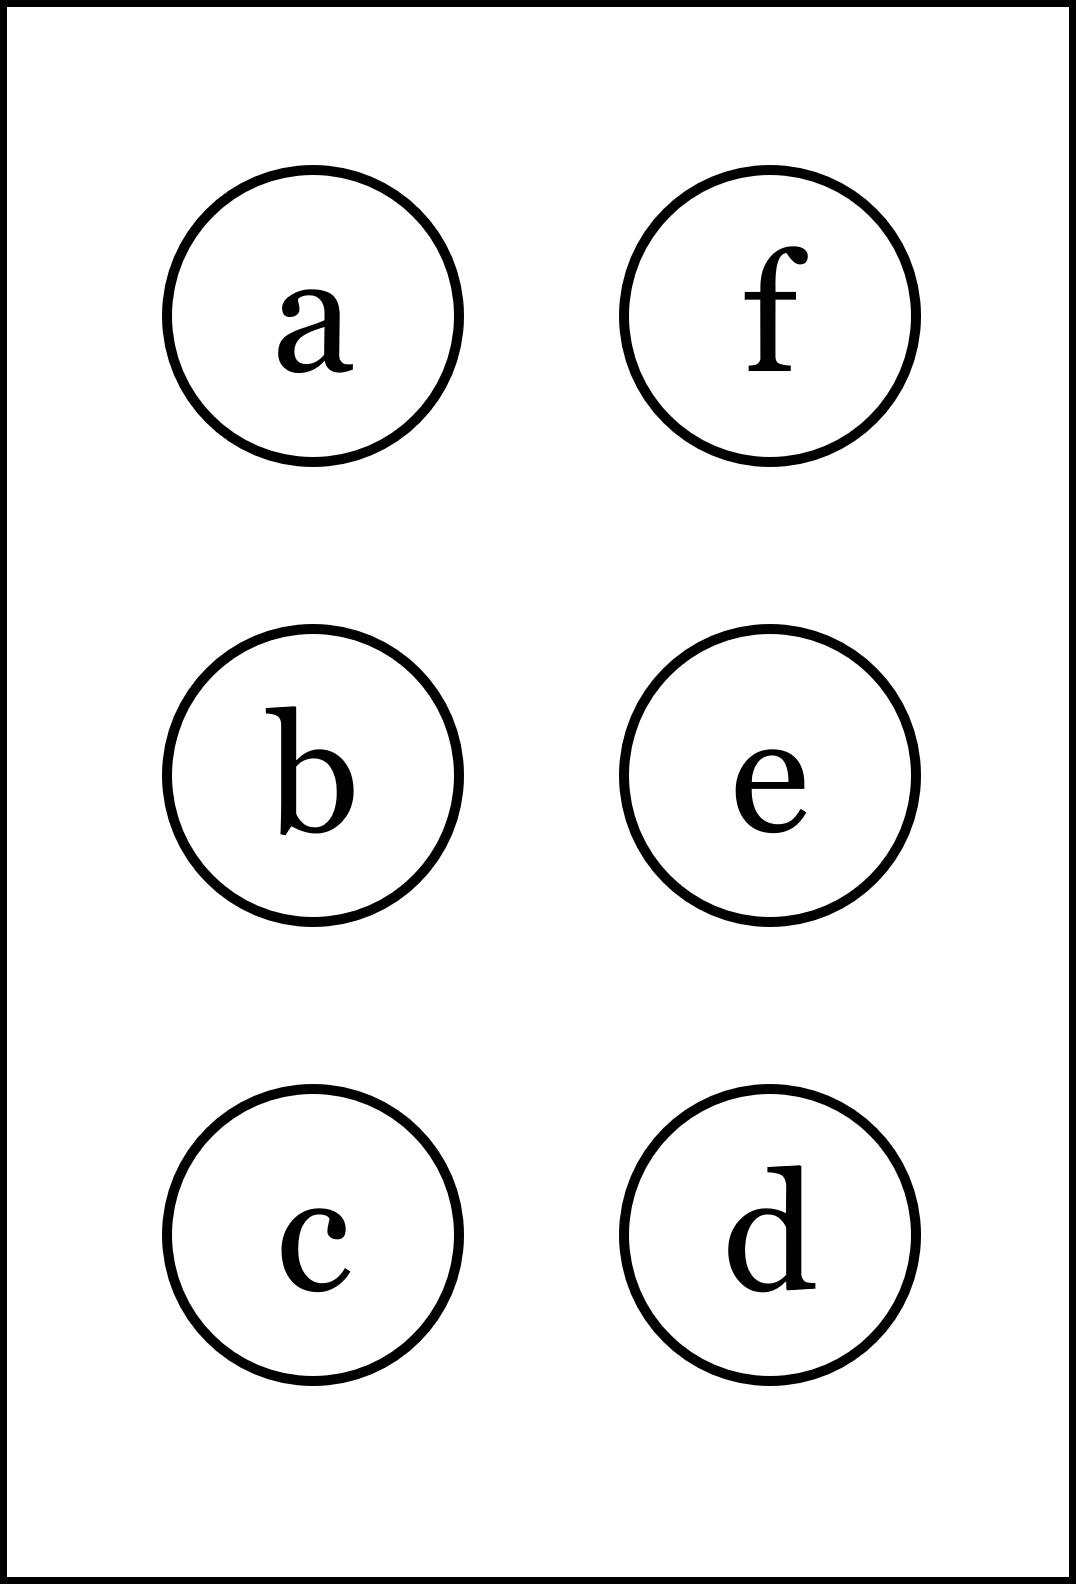
\includegraphics[height=40mm]{../images/braille.png}
{\small Písmeno Braillovej abecedy}
\end{center}
\end{minipage}
\end{center}
\end{minipage}

\end{tabular}
\begin{tikzpicture}[remember picture,overlay]\node[xshift=7mm,yshift=-100.6mm,anchor=north west] at (current page.north west){\ding{33}};\end{tikzpicture}
\begin{tikzpicture}[remember picture,overlay]\node[xshift=151.2mm,yshift=-7mm,anchor=north west,rotate=270] at (current page.north west){\ding{33}};\end{tikzpicture}
\clearpage
\thispagestyle{empty}
\begin{tabular}{c:c}
\begin{minipage}[c][99mm][t]{0.49\linewidth}
\begin{center}
\vspace{7mm}
{\huge Kubická rovnice, skupina \textit{Lambda $\lambda$} -\romannumeral1}\\[4.5mm]
\textit{Meno:}\phantom{xxxxxxxxxxxxxxxxxxxxxxxxxxxxxxxxxxxxxxxxxxxxxxxxxxxxxxxxxxxxxxxxx}\\[3.5mm]
\textbf{Vypočítej součet kořenů kubické rovnice.} Dvojitý kořen považuj do součtu za dva.\\Analogicky pro trojitý kořen. Pokud ti vyjde stejný výsledek jako je za otazníky, tak\\napravo obarvi příslušející kroužek načerno. \textbf{Spolu odevzdejte výsledné slovo}.\\[3mm]
\begin{minipage}{0.77\linewidth}
\begin{center}
\begin{varwidth}{\textwidth}
\begin{enumerate}
\large
\item $x^3-6x^2+8x=0$\quad \dotfill\; ???\;\dotfill \quad -2
\item $2x^3-4x^2-22x+24=0$\quad \dotfill\; ???\;\dotfill \quad 2
\item $-24x^3+34x^2-6x-4=0$\quad \dotfill\; ???\;\dotfill \quad $\nicefrac{17}{12}$
\item $2x^3-5x^2-26x+56=0$\quad \dotfill\; ???\;\dotfill \quad $\nicefrac{19}{2}$
\item \quad \dotfill\; ???\;\dotfill \quad vybarvi
\item \quad \dotfill\; ???\;\dotfill \quad vybarvi
\end{enumerate}
\end{varwidth}
\end{center}
\end{minipage}
\begin{minipage}{0.20\linewidth}
\begin{center}
{\Huge\bfseries 1.} \\[2mm]
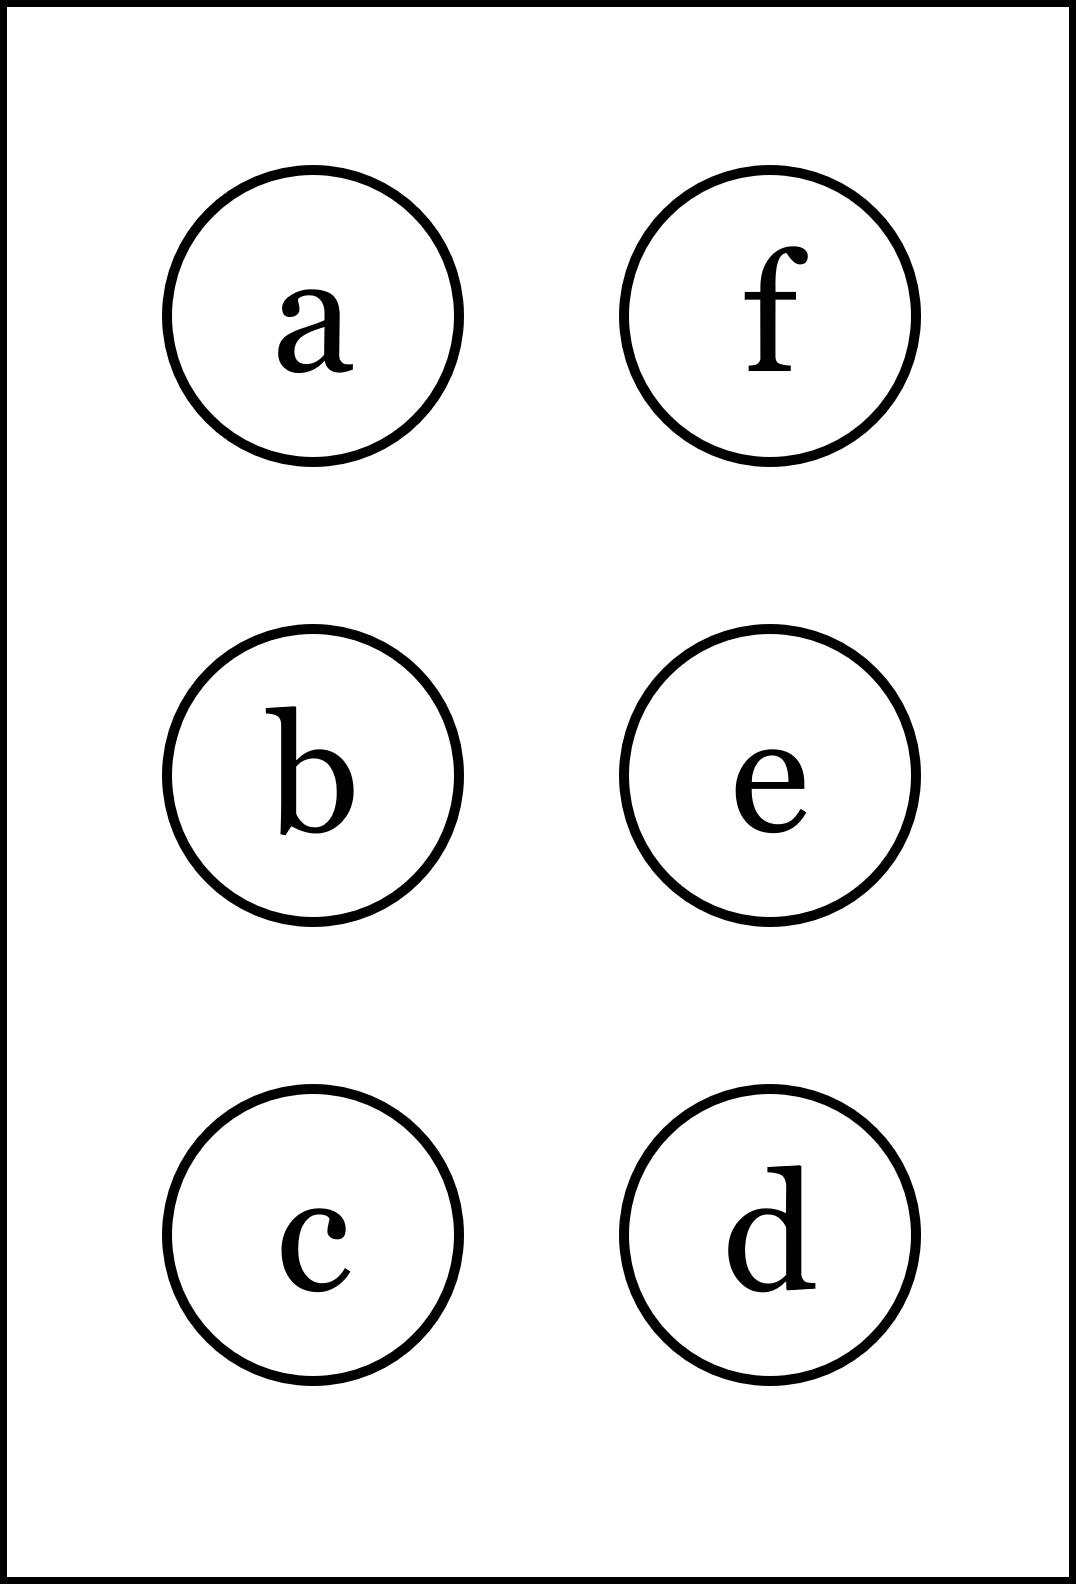
\includegraphics[height=40mm]{../images/braille.png}
{\small Písmeno Braillovej abecedy}
\end{center}
\end{minipage}
\end{center}
\end{minipage}
&
\begin{minipage}[c][99mm][t]{0.49\linewidth}
\begin{center}
\vspace{7mm}
{\huge Kubická rovnice, skupina \textit{Lambda $\lambda$} -\romannumeral2}\\[4.5mm]
\textit{Meno:}\phantom{xxxxxxxxxxxxxxxxxxxxxxxxxxxxxxxxxxxxxxxxxxxxxxxxxxxxxxxxxxxxxxxxx}\\[3.5mm]
\textbf{Vypočítej součet kořenů kubické rovnice.} Dvojitý kořen považuj do součtu za dva.\\Analogicky pro trojitý kořen. Pokud ti vyjde stejný výsledek jako je za otazníky, tak\\napravo obarvi příslušející kroužek načerno. \textbf{Spolu odevzdejte výsledné slovo}.\\[3mm]
\begin{minipage}{0.77\linewidth}
\begin{center}
\begin{varwidth}{\textwidth}
\begin{enumerate}
\large
\item $2x^3-2x^2-12x=0$\quad \dotfill\; ???\;\dotfill \quad 1
\item $x^3-3x^2-25x-21=0$\quad \dotfill\; ???\;\dotfill \quad 9
\item $-8x^3+52x^2+32x-28=0$\quad \dotfill\; ???\;\dotfill \quad $\nicefrac{-17}{2}$
\item $10x^3-38x^2-16x+32=0$\quad \dotfill\; ???\;\dotfill \quad $\nicefrac{19}{5}$
\item \quad \dotfill\; ???\;\dotfill \quad nebarvi
\item \quad \dotfill\; ???\;\dotfill \quad nebarvi
\end{enumerate}
\end{varwidth}
\end{center}
\end{minipage}
\begin{minipage}{0.20\linewidth}
\begin{center}
{\Huge\bfseries 2.} \\[2mm]
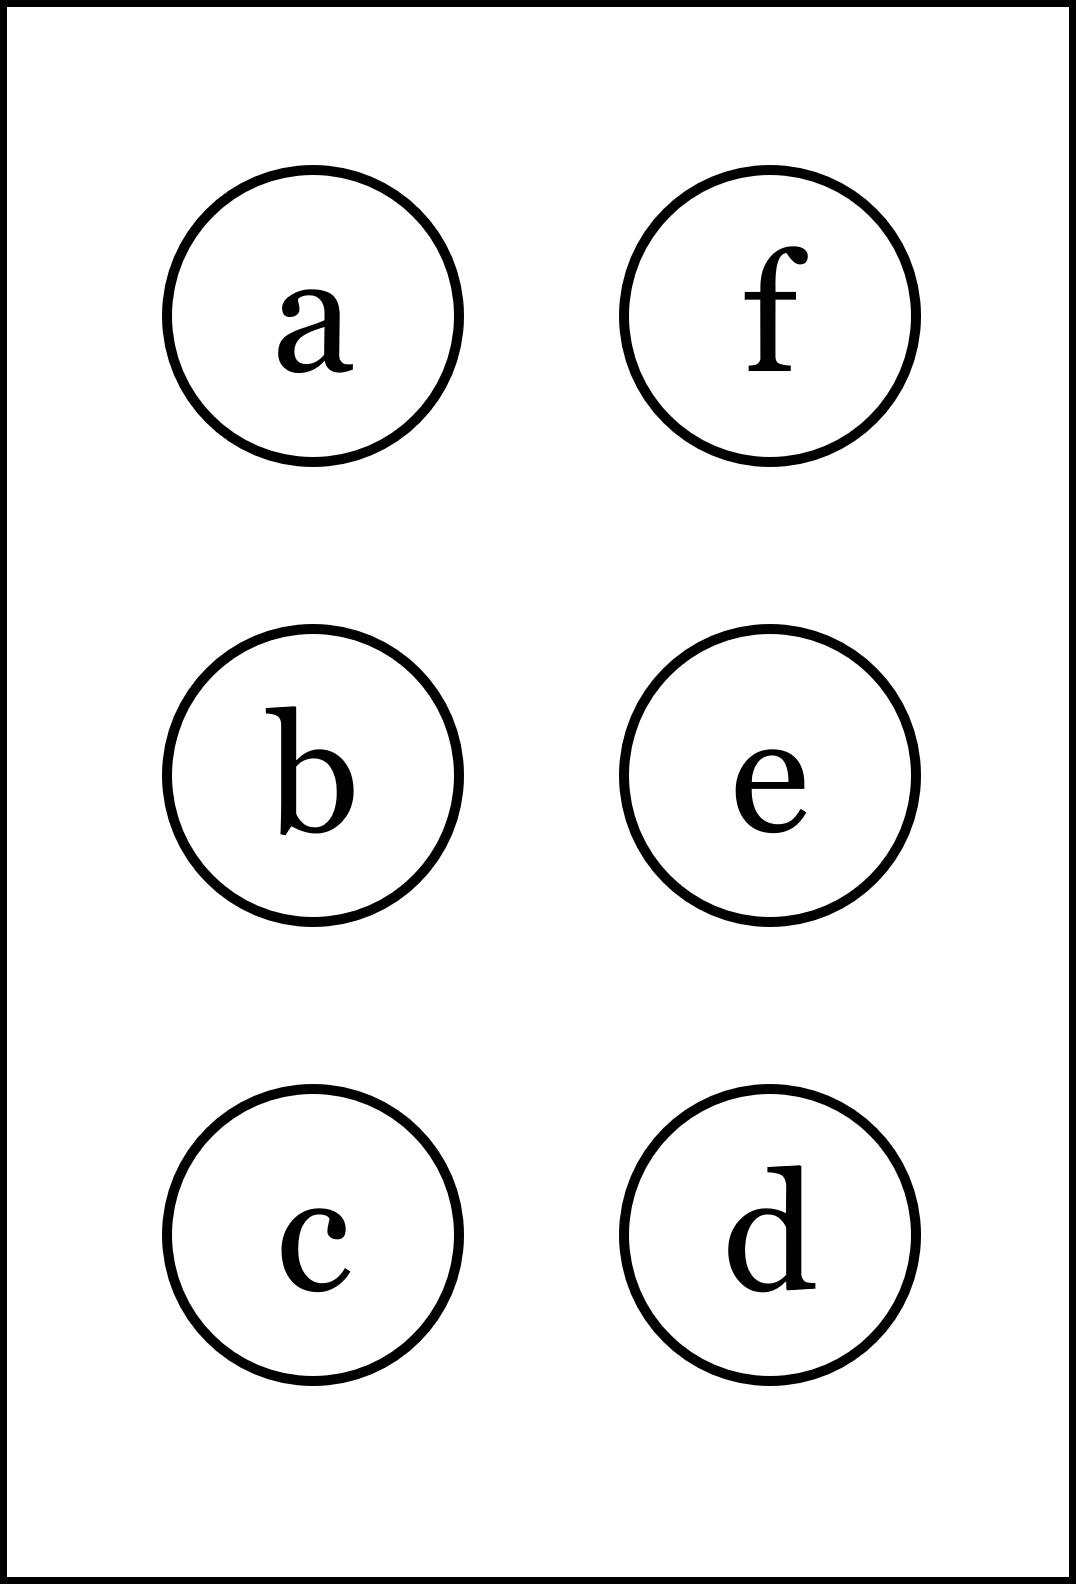
\includegraphics[height=40mm]{../images/braille.png}
{\small Písmeno Braillovej abecedy}
\end{center}
\end{minipage}
\end{center}
\end{minipage}
\\ \hdashline
\begin{minipage}[c][99mm][t]{0.49\linewidth}
\begin{center}
\vspace{7mm}
{\huge Kubická rovnice, skupina \textit{Lambda $\lambda$} -\romannumeral3}\\[4.5mm]
\textit{Meno:}\phantom{xxxxxxxxxxxxxxxxxxxxxxxxxxxxxxxxxxxxxxxxxxxxxxxxxxxxxxxxxxxxxxxxx}\\[3.5mm]
\textbf{Vypočítej součet kořenů kubické rovnice.} Dvojitý kořen považuj do součtu za dva.\\Analogicky pro trojitý kořen. Pokud ti vyjde stejný výsledek jako je za otazníky, tak\\napravo obarvi příslušející kroužek načerno. \textbf{Spolu odevzdejte výsledné slovo}.\\[3mm]
\begin{minipage}{0.77\linewidth}
\begin{center}
\begin{varwidth}{\textwidth}
\begin{enumerate}
\large
\item $3x^3+18x^2-21x=0$\quad \dotfill\; ???\;\dotfill \quad -8
\item $9x^3-36x^2-9x+36=0$\quad \dotfill\; ???\;\dotfill \quad 4
\item $-8x^3+7x^2+32x-28=0$\quad \dotfill\; ???\;\dotfill \quad $\nicefrac{7}{8}$
\item $2x^3-24x-32=0$\quad \dotfill\; ???\;\dotfill \quad 4
\item \quad \dotfill\; ???\;\dotfill \quad vybarvi
\item \quad \dotfill\; ???\;\dotfill \quad vybarvi
\end{enumerate}
\end{varwidth}
\end{center}
\end{minipage}
\begin{minipage}{0.20\linewidth}
\begin{center}
{\Huge\bfseries 3.} \\[2mm]
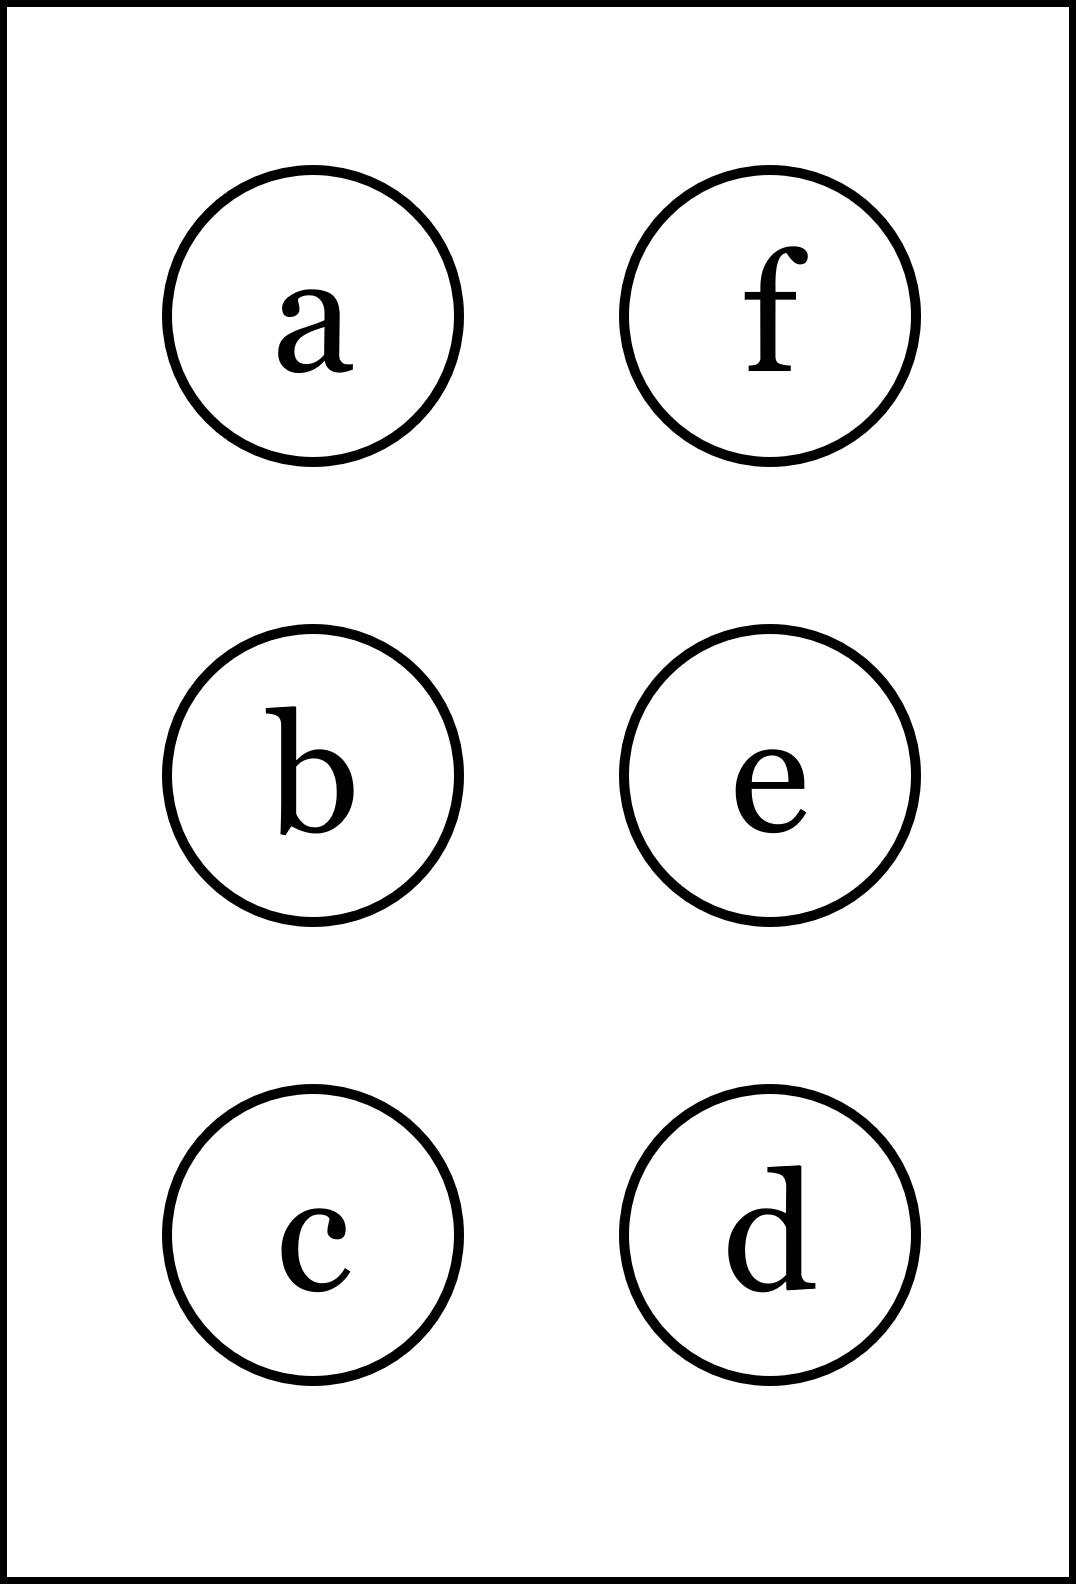
\includegraphics[height=40mm]{../images/braille.png}
{\small Písmeno Braillovej abecedy}
\end{center}
\end{minipage}
\end{center}
\end{minipage}
&
\begin{minipage}[c][99mm][t]{0.49\linewidth}
\begin{center}
\vspace{7mm}
{\huge Kubická rovnice, skupina \textit{Lambda $\lambda$} -\romannumeral4}\\[4.5mm]
\textit{Meno:}\phantom{xxxxxxxxxxxxxxxxxxxxxxxxxxxxxxxxxxxxxxxxxxxxxxxxxxxxxxxxxxxxxxxxx}\\[3.5mm]
\textbf{Vypočítej součet kořenů kubické rovnice.} Dvojitý kořen považuj do součtu za dva.\\Analogicky pro trojitý kořen. Pokud ti vyjde stejný výsledek jako je za otazníky, tak\\napravo obarvi příslušející kroužek načerno. \textbf{Spolu odevzdejte výsledné slovo}.\\[3mm]
\begin{minipage}{0.77\linewidth}
\begin{center}
\begin{varwidth}{\textwidth}
\begin{enumerate}
\large
\item $x^3-7x^2+10x=0$\quad \dotfill\; ???\;\dotfill \quad 7
\item $-5x^3-10x^2+35x-20=0$\quad \dotfill\; ???\;\dotfill \quad -6
\item $-16x^3+64x^2-43x-15=0$\quad \dotfill\; ???\;\dotfill \quad $\nicefrac{-3}{2}$
\item $-7x^3+18x^2+37x+12=0$\quad \dotfill\; ???\;\dotfill \quad $\nicefrac{38}{7}$
\item \quad \dotfill\; ???\;\dotfill \quad nebarvi
\item \quad \dotfill\; ???\;\dotfill \quad nebarvi
\end{enumerate}
\end{varwidth}
\end{center}
\end{minipage}
\begin{minipage}{0.20\linewidth}
\begin{center}
{\Huge\bfseries 4.} \\[2mm]
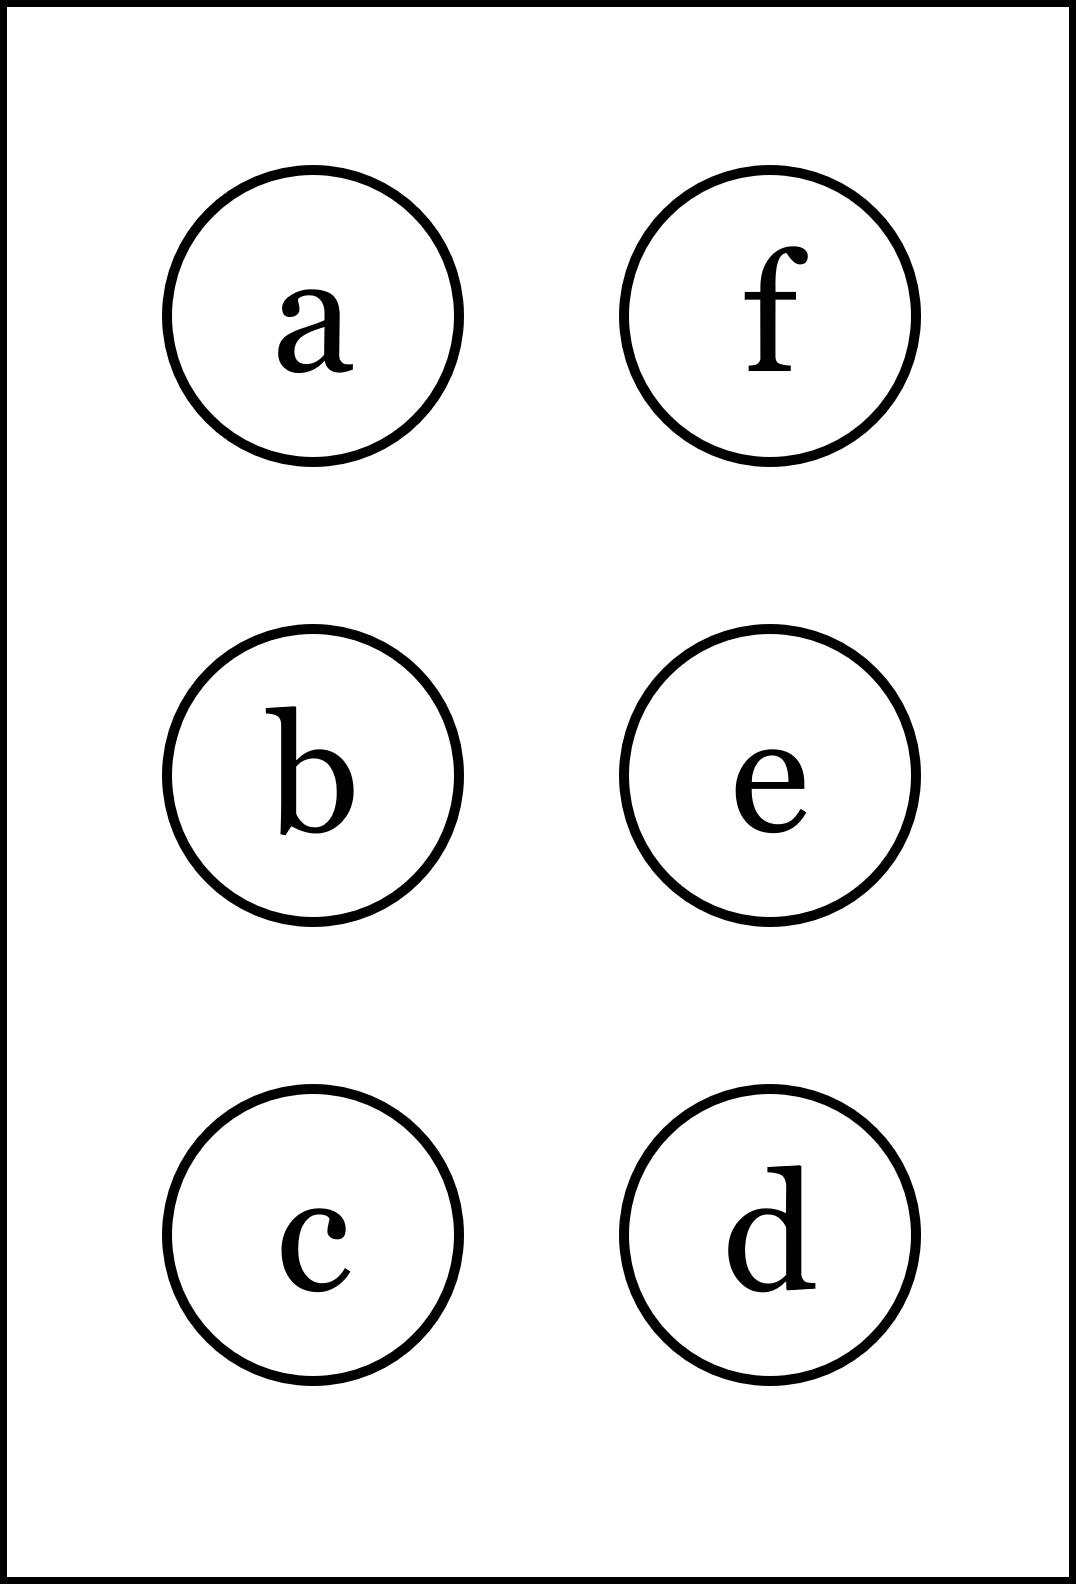
\includegraphics[height=40mm]{../images/braille.png}
{\small Písmeno Braillovej abecedy}
\end{center}
\end{minipage}
\end{center}
\end{minipage}

\end{tabular}
\begin{tikzpicture}[remember picture,overlay]\node[xshift=7mm,yshift=-100.6mm,anchor=north west] at (current page.north west){\ding{33}};\end{tikzpicture}
\begin{tikzpicture}[remember picture,overlay]\node[xshift=151.2mm,yshift=-7mm,anchor=north west,rotate=270] at (current page.north west){\ding{33}};\end{tikzpicture}
\clearpage
\thispagestyle{empty}
\begin{tabular}{c:c}
\begin{minipage}[c][99mm][t]{0.49\linewidth}
\begin{center}
\vspace{7mm}
{\huge Kubická rovnice, skupina \textit{Mu $\mu$} -\romannumeral1}\\[4.5mm]
\textit{Meno:}\phantom{xxxxxxxxxxxxxxxxxxxxxxxxxxxxxxxxxxxxxxxxxxxxxxxxxxxxxxxxxxxxxxxxx}\\[3.5mm]
\textbf{Vypočítej součet kořenů kubické rovnice.} Dvojitý kořen považuj do součtu za dva.\\Analogicky pro trojitý kořen. Pokud ti vyjde stejný výsledek jako je za otazníky, tak\\napravo obarvi příslušející kroužek načerno. \textbf{Spolu odevzdejte výsledné slovo}.\\[3mm]
\begin{minipage}{0.77\linewidth}
\begin{center}
\begin{varwidth}{\textwidth}
\begin{enumerate}
\large
\item $-x^3-4x^2+5x=0$\quad \dotfill\; ???\;\dotfill \quad -4
\item $2x^3+2x^2-28x-48=0$\quad \dotfill\; ???\;\dotfill \quad -9
\item $-4x^3+2x^2+24x+18=0$\quad \dotfill\; ???\;\dotfill \quad $\nicefrac{11}{2}$
\item $3x^3-x^2-38x-24=0$\quad \dotfill\; ???\;\dotfill \quad $\nicefrac{1}{3}$
\item \quad \dotfill\; ???\;\dotfill \quad vybarvi
\item \quad \dotfill\; ???\;\dotfill \quad nebarvi
\end{enumerate}
\end{varwidth}
\end{center}
\end{minipage}
\begin{minipage}{0.20\linewidth}
\begin{center}
{\Huge\bfseries 1.} \\[2mm]
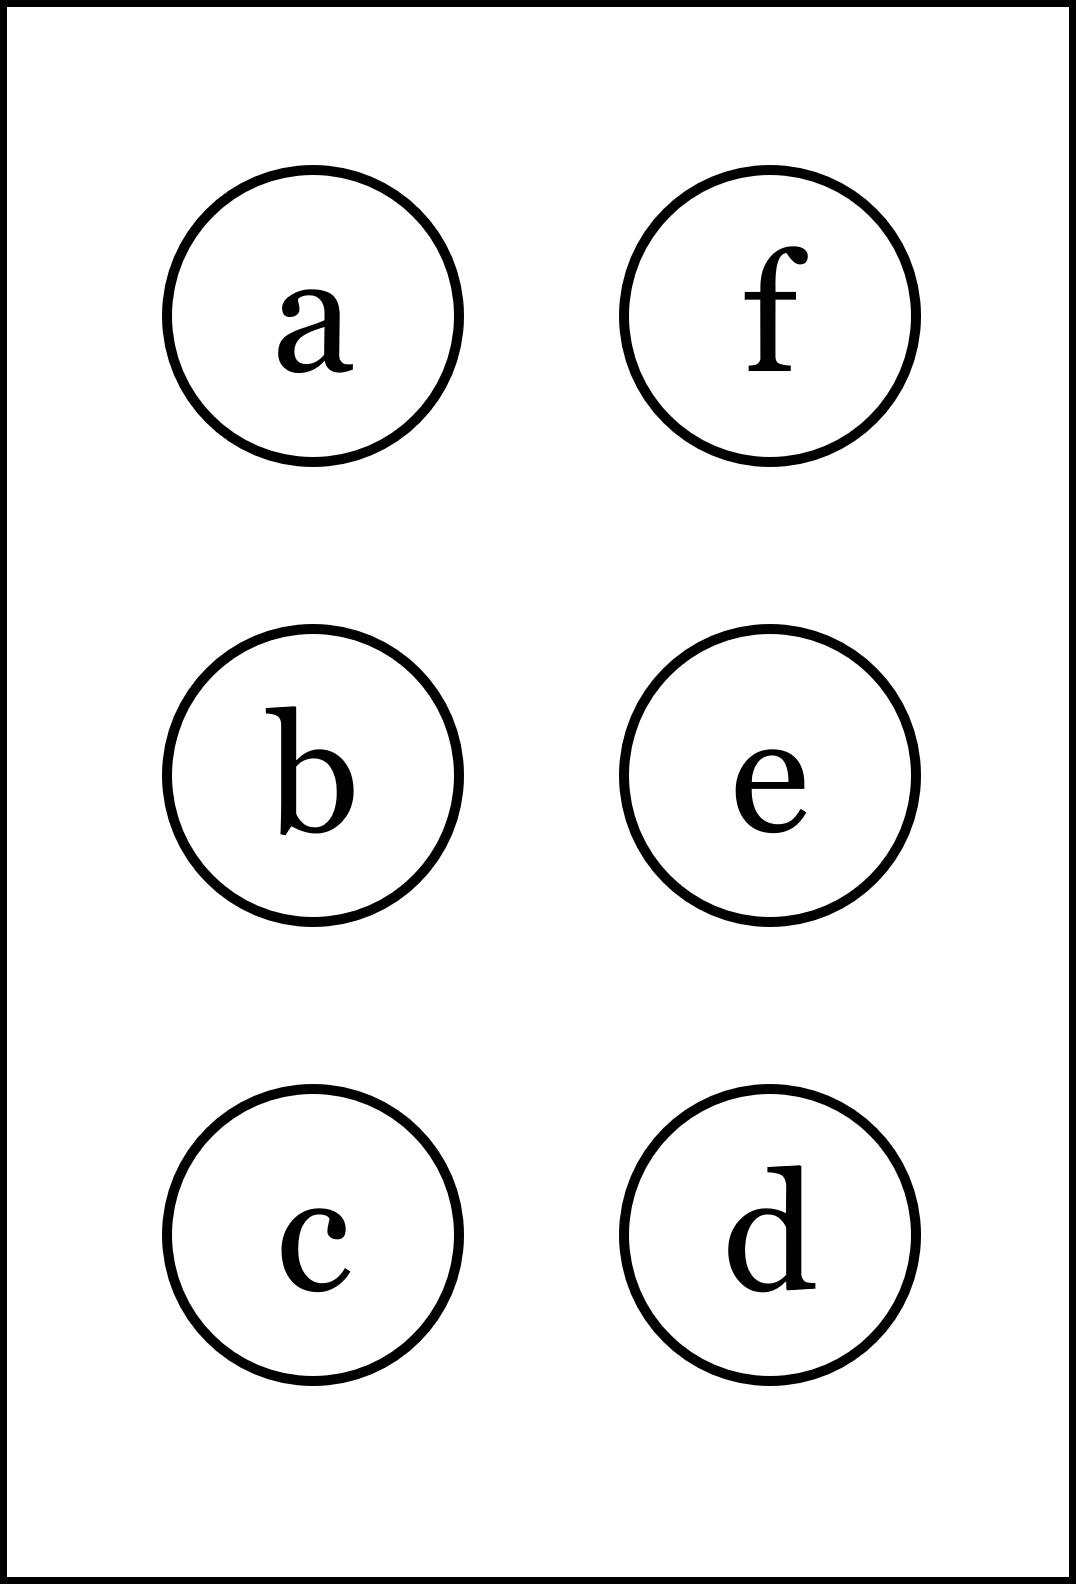
\includegraphics[height=40mm]{../images/braille.png}
{\small Písmeno Braillovej abecedy}
\end{center}
\end{minipage}
\end{center}
\end{minipage}
&
\begin{minipage}[c][99mm][t]{0.49\linewidth}
\begin{center}
\vspace{7mm}
{\huge Kubická rovnice, skupina \textit{Mu $\mu$} -\romannumeral2}\\[4.5mm]
\textit{Meno:}\phantom{xxxxxxxxxxxxxxxxxxxxxxxxxxxxxxxxxxxxxxxxxxxxxxxxxxxxxxxxxxxxxxxxx}\\[3.5mm]
\textbf{Vypočítej součet kořenů kubické rovnice.} Dvojitý kořen považuj do součtu za dva.\\Analogicky pro trojitý kořen. Pokud ti vyjde stejný výsledek jako je za otazníky, tak\\napravo obarvi příslušející kroužek načerno. \textbf{Spolu odevzdejte výsledné slovo}.\\[3mm]
\begin{minipage}{0.77\linewidth}
\begin{center}
\begin{varwidth}{\textwidth}
\begin{enumerate}
\large
\item $-2x^3-4x^2+16x=0$\quad \dotfill\; ???\;\dotfill \quad -2
\item $2x^3+4x^2-2x-4=0$\quad \dotfill\; ???\;\dotfill \quad 4
\item $-8x^3-12x^2+8x+12=0$\quad \dotfill\; ???\;\dotfill \quad $\nicefrac{-3}{2}$
\item $16x^3+52x^2+10x-6=0$\quad \dotfill\; ???\;\dotfill \quad $\nicefrac{9}{4}$
\item \quad \dotfill\; ???\;\dotfill \quad vybarvi
\item \quad \dotfill\; ???\;\dotfill \quad vybarvi
\end{enumerate}
\end{varwidth}
\end{center}
\end{minipage}
\begin{minipage}{0.20\linewidth}
\begin{center}
{\Huge\bfseries 2.} \\[2mm]
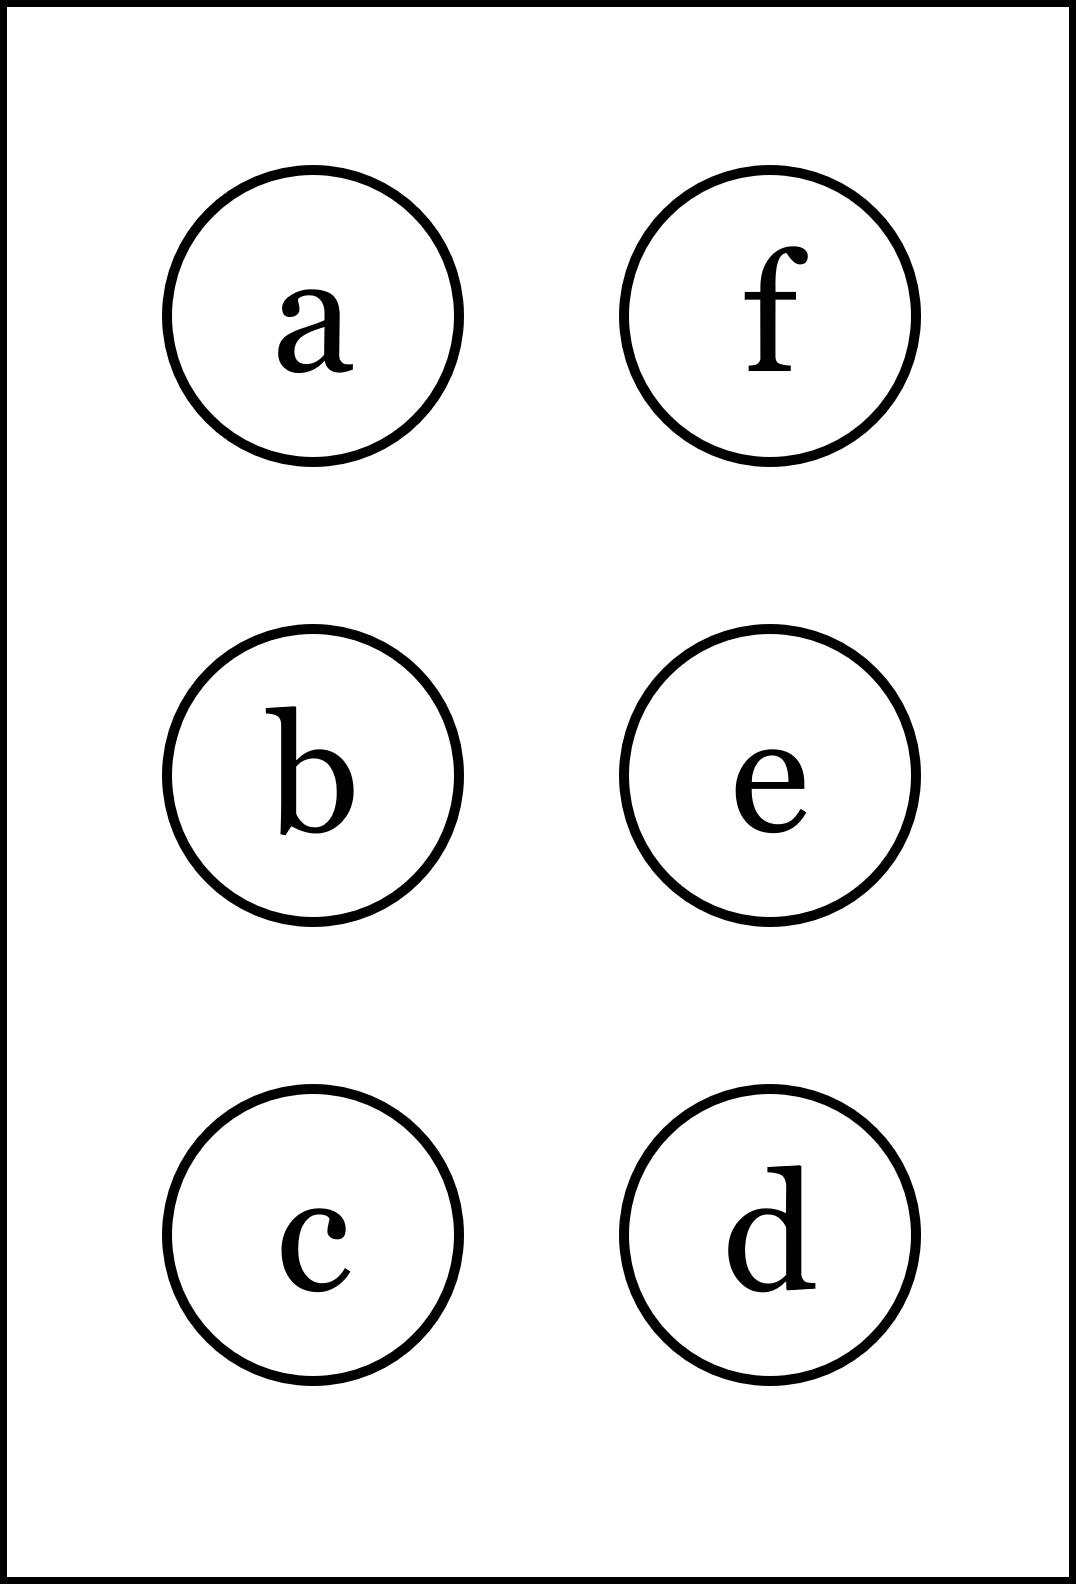
\includegraphics[height=40mm]{../images/braille.png}
{\small Písmeno Braillovej abecedy}
\end{center}
\end{minipage}
\end{center}
\end{minipage}
\\ \hdashline
\begin{minipage}[c][99mm][t]{0.49\linewidth}
\begin{center}
\vspace{7mm}
{\huge Kubická rovnice, skupina \textit{Mu $\mu$} -\romannumeral3}\\[4.5mm]
\textit{Meno:}\phantom{xxxxxxxxxxxxxxxxxxxxxxxxxxxxxxxxxxxxxxxxxxxxxxxxxxxxxxxxxxxxxxxxx}\\[3.5mm]
\textbf{Vypočítej součet kořenů kubické rovnice.} Dvojitý kořen považuj do součtu za dva.\\Analogicky pro trojitý kořen. Pokud ti vyjde stejný výsledek jako je za otazníky, tak\\napravo obarvi příslušející kroužek načerno. \textbf{Spolu odevzdejte výsledné slovo}.\\[3mm]
\begin{minipage}{0.77\linewidth}
\begin{center}
\begin{varwidth}{\textwidth}
\begin{enumerate}
\large
\item $x^3+5x^2+6x=0$\quad \dotfill\; ???\;\dotfill \quad -5
\item $-x^3-4x^2+15x+18=0$\quad \dotfill\; ???\;\dotfill \quad 8
\item $-28x^3+46x^2-2x-16=0$\quad \dotfill\; ???\;\dotfill \quad $\nicefrac{-9}{14}$
\item $-18x^3-50x^2-24x+8=0$\quad \dotfill\; ???\;\dotfill \quad $\nicefrac{7}{9}$
\item \quad \dotfill\; ???\;\dotfill \quad vybarvi
\item \quad \dotfill\; ???\;\dotfill \quad nebarvi
\end{enumerate}
\end{varwidth}
\end{center}
\end{minipage}
\begin{minipage}{0.20\linewidth}
\begin{center}
{\Huge\bfseries 3.} \\[2mm]
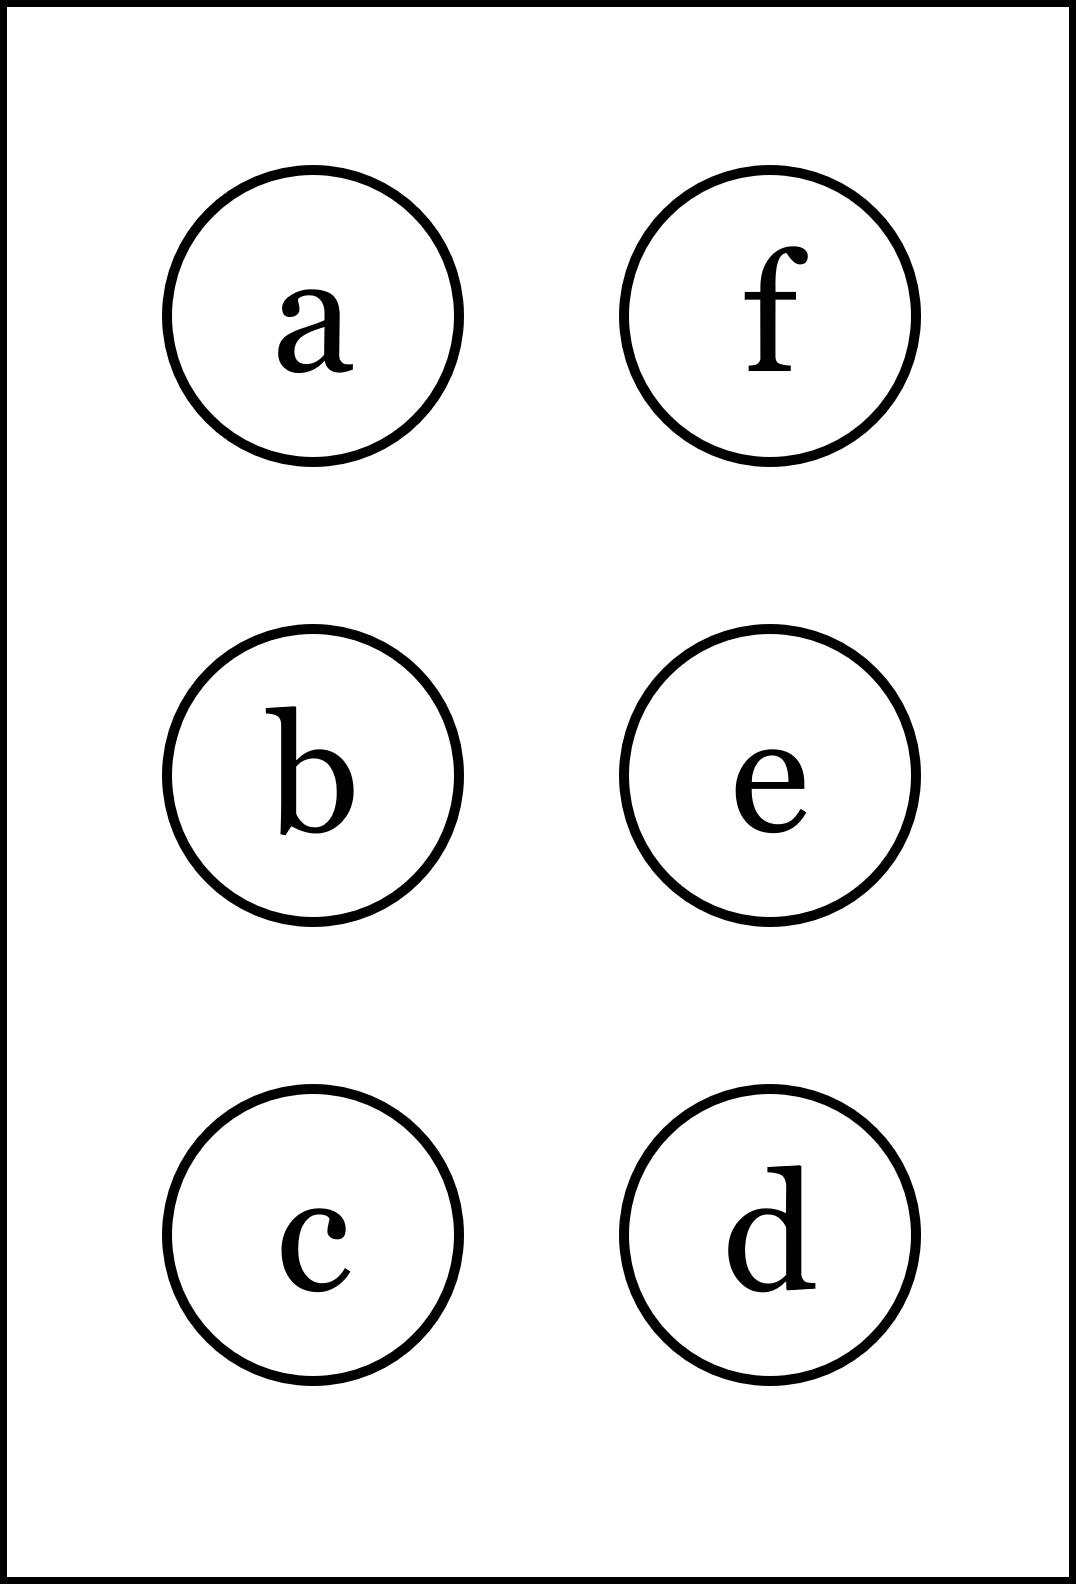
\includegraphics[height=40mm]{../images/braille.png}
{\small Písmeno Braillovej abecedy}
\end{center}
\end{minipage}
\end{center}
\end{minipage}
&
\begin{minipage}[c][99mm][t]{0.49\linewidth}
\begin{center}
\vspace{7mm}
{\huge Kubická rovnice, skupina \textit{Mu $\mu$} -\romannumeral4}\\[4.5mm]
\textit{Meno:}\phantom{xxxxxxxxxxxxxxxxxxxxxxxxxxxxxxxxxxxxxxxxxxxxxxxxxxxxxxxxxxxxxxxxx}\\[3.5mm]
\textbf{Vypočítej součet kořenů kubické rovnice.} Dvojitý kořen považuj do součtu za dva.\\Analogicky pro trojitý kořen. Pokud ti vyjde stejný výsledek jako je za otazníky, tak\\napravo obarvi příslušející kroužek načerno. \textbf{Spolu odevzdejte výsledné slovo}.\\[3mm]
\begin{minipage}{0.77\linewidth}
\begin{center}
\begin{varwidth}{\textwidth}
\begin{enumerate}
\large
\item $x^3-3x^2-4x=0$\quad \dotfill\; ???\;\dotfill \quad 3
\item $-x^3-8x^2-9x+18=0$\quad \dotfill\; ???\;\dotfill \quad 10
\item $-6x^3-39x^2-39x+30=0$\quad \dotfill\; ???\;\dotfill \quad $\nicefrac{-13}{2}$
\item $-10x^3-37x^2-22x-3=0$\quad \dotfill\; ???\;\dotfill \quad $\nicefrac{27}{10}$
\item \quad \dotfill\; ???\;\dotfill \quad nebarvi
\item \quad \dotfill\; ???\;\dotfill \quad nebarvi
\end{enumerate}
\end{varwidth}
\end{center}
\end{minipage}
\begin{minipage}{0.20\linewidth}
\begin{center}
{\Huge\bfseries 4.} \\[2mm]
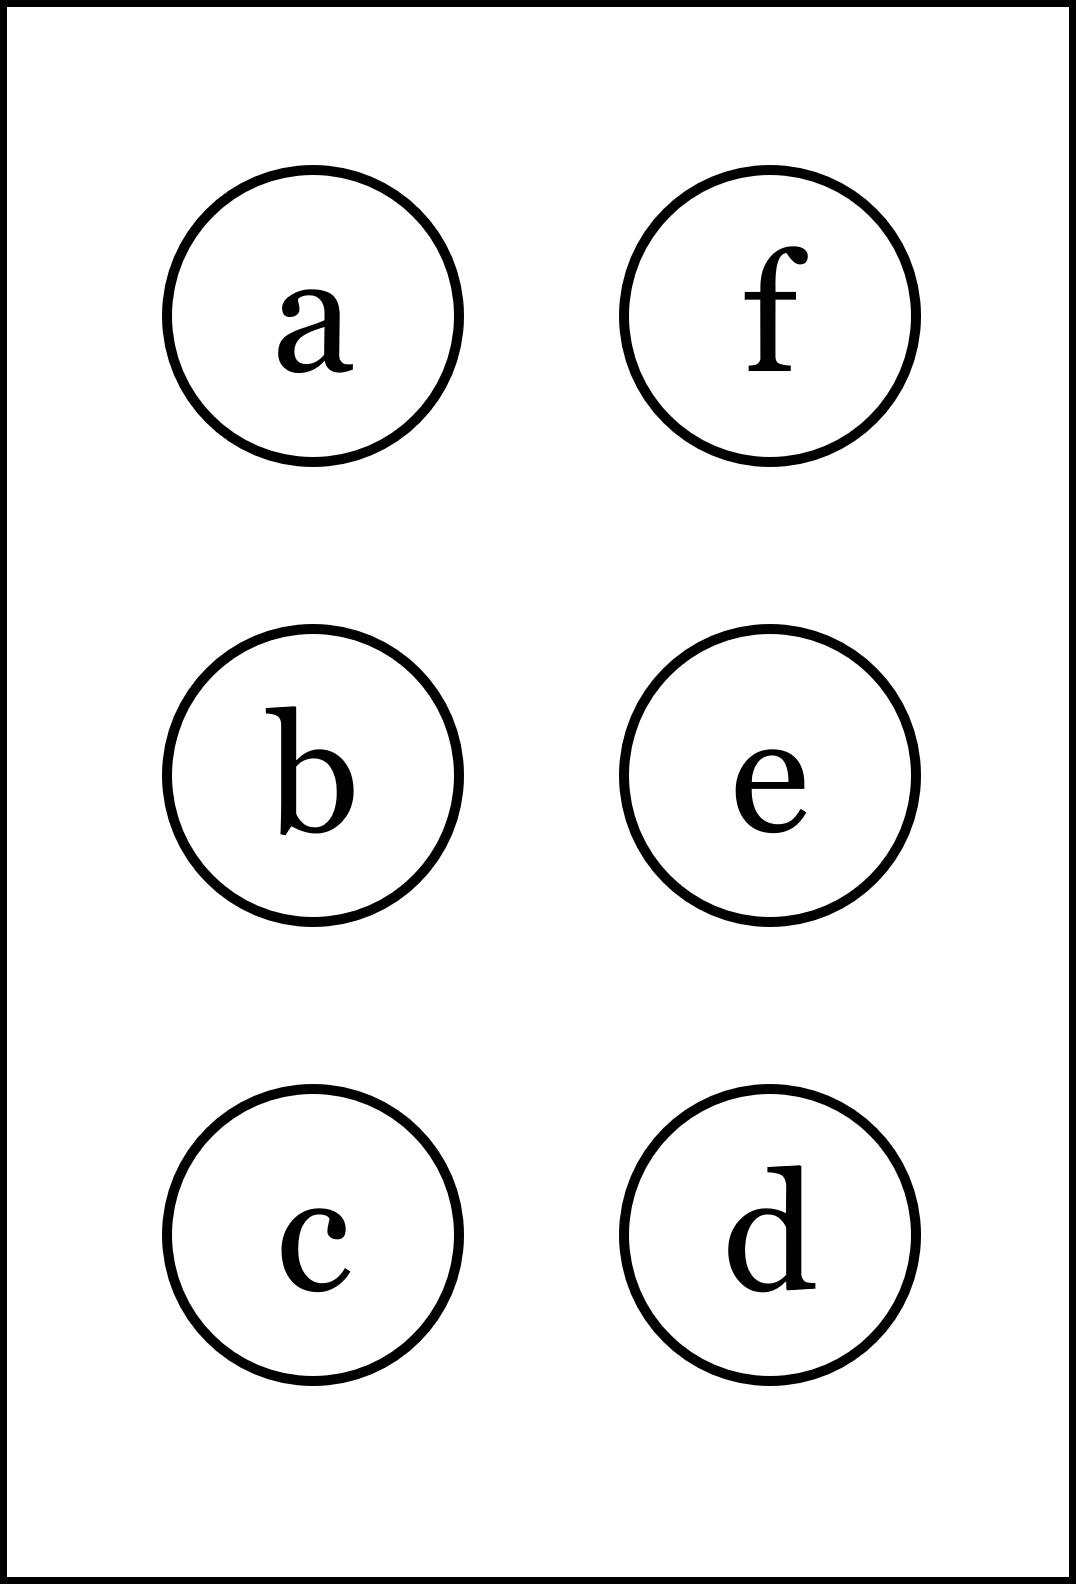
\includegraphics[height=40mm]{../images/braille.png}
{\small Písmeno Braillovej abecedy}
\end{center}
\end{minipage}
\end{center}
\end{minipage}

\end{tabular}
\begin{tikzpicture}[remember picture,overlay]\node[xshift=7mm,yshift=-100.6mm,anchor=north west] at (current page.north west){\ding{33}};\end{tikzpicture}
\begin{tikzpicture}[remember picture,overlay]\node[xshift=151.2mm,yshift=-7mm,anchor=north west,rotate=270] at (current page.north west){\ding{33}};\end{tikzpicture}
\clearpage
\thispagestyle{empty}
\begin{tabular}{c:c}
\begin{minipage}[c][99mm][t]{0.49\linewidth}
\begin{center}
\vspace{7mm}
{\huge Kubická rovnice, skupina \textit{Nu $\nu$} -\romannumeral1}\\[4.5mm]
\textit{Meno:}\phantom{xxxxxxxxxxxxxxxxxxxxxxxxxxxxxxxxxxxxxxxxxxxxxxxxxxxxxxxxxxxxxxxxx}\\[3.5mm]
\textbf{Vypočítej součet kořenů kubické rovnice.} Dvojitý kořen považuj do součtu za dva.\\Analogicky pro trojitý kořen. Pokud ti vyjde stejný výsledek jako je za otazníky, tak\\napravo obarvi příslušející kroužek načerno. \textbf{Spolu odevzdejte výsledné slovo}.\\[3mm]
\begin{minipage}{0.77\linewidth}
\begin{center}
\begin{varwidth}{\textwidth}
\begin{enumerate}
\large
\item $-3x^3+15x^2-12x=0$\quad \dotfill\; ???\;\dotfill \quad -3
\item $-2x^3+14x^2-22x+10=0$\quad \dotfill\; ???\;\dotfill \quad 7
\item $-3x^3-22x^2-43x-12=0$\quad \dotfill\; ???\;\dotfill \quad $\nicefrac{20}{3}$
\item $8x^3-22x^2+10x+4=0$\quad \dotfill\; ???\;\dotfill \quad $\nicefrac{3}{4}$
\item \quad \dotfill\; ???\;\dotfill \quad vybarvi
\item \quad \dotfill\; ???\;\dotfill \quad vybarvi
\end{enumerate}
\end{varwidth}
\end{center}
\end{minipage}
\begin{minipage}{0.20\linewidth}
\begin{center}
{\Huge\bfseries 1.} \\[2mm]
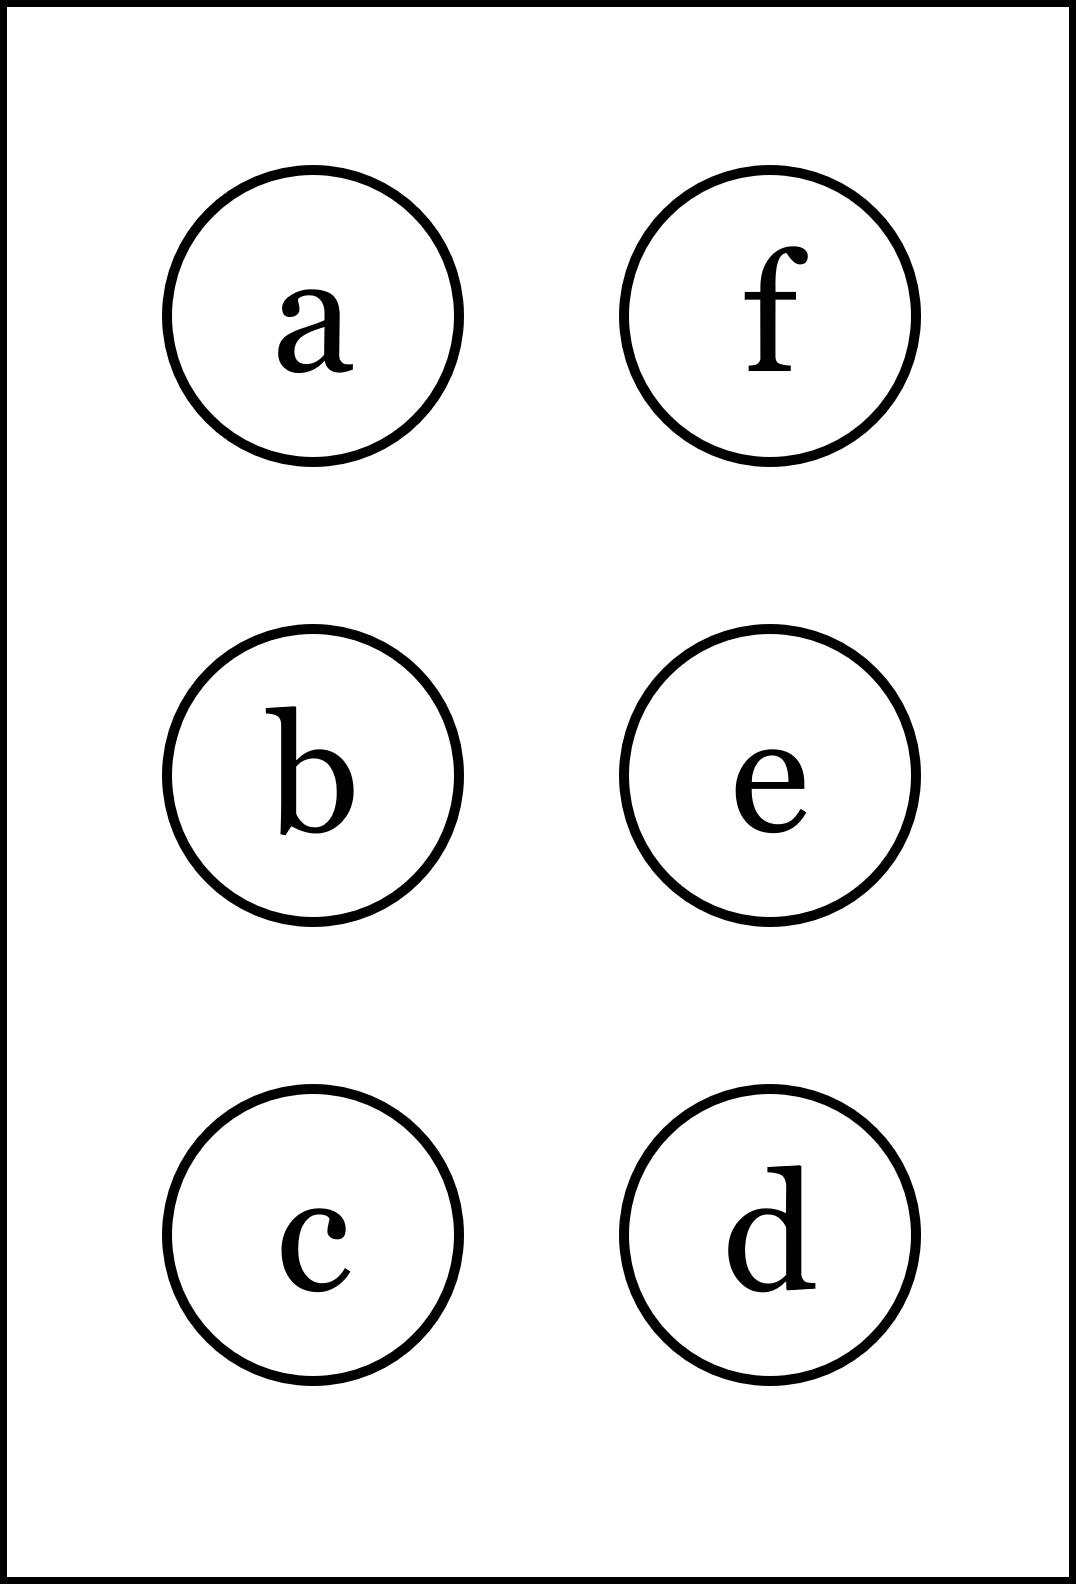
\includegraphics[height=40mm]{../images/braille.png}
{\small Písmeno Braillovej abecedy}
\end{center}
\end{minipage}
\end{center}
\end{minipage}
&
\begin{minipage}[c][99mm][t]{0.49\linewidth}
\begin{center}
\vspace{7mm}
{\huge Kubická rovnice, skupina \textit{Nu $\nu$} -\romannumeral2}\\[4.5mm]
\textit{Meno:}\phantom{xxxxxxxxxxxxxxxxxxxxxxxxxxxxxxxxxxxxxxxxxxxxxxxxxxxxxxxxxxxxxxxxx}\\[3.5mm]
\textbf{Vypočítej součet kořenů kubické rovnice.} Dvojitý kořen považuj do součtu za dva.\\Analogicky pro trojitý kořen. Pokud ti vyjde stejný výsledek jako je za otazníky, tak\\napravo obarvi příslušející kroužek načerno. \textbf{Spolu odevzdejte výsledné slovo}.\\[3mm]
\begin{minipage}{0.77\linewidth}
\begin{center}
\begin{varwidth}{\textwidth}
\begin{enumerate}
\large
\item $-x^3+4x^2+12x=0$\quad \dotfill\; ???\;\dotfill \quad 4
\item $-x^3-5x^2+9x+45=0$\quad \dotfill\; ???\;\dotfill \quad 11
\item $32x^3-36x^2-47x+21=0$\quad \dotfill\; ???\;\dotfill \quad $\nicefrac{-19}{8}$
\item $40x^3+49x^2-x-10=0$\quad \dotfill\; ???\;\dotfill \quad $\nicefrac{-49}{40}$
\item \quad \dotfill\; ???\;\dotfill \quad nebarvi
\item \quad \dotfill\; ???\;\dotfill \quad nebarvi
\end{enumerate}
\end{varwidth}
\end{center}
\end{minipage}
\begin{minipage}{0.20\linewidth}
\begin{center}
{\Huge\bfseries 2.} \\[2mm]
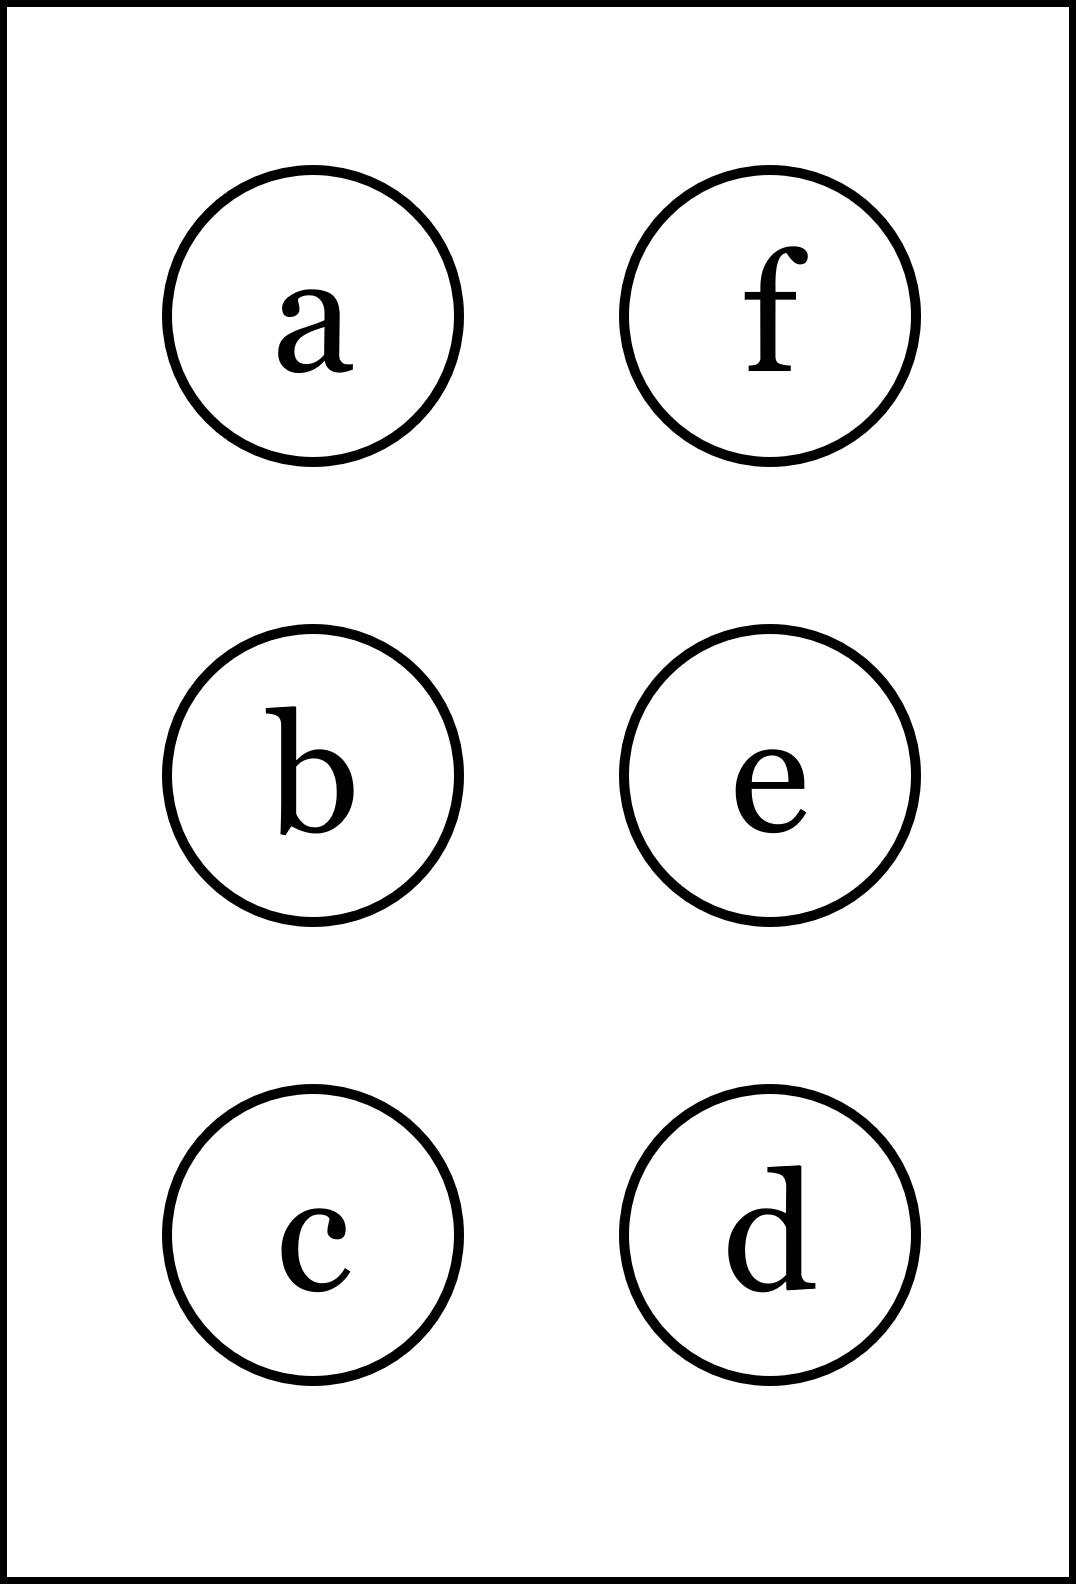
\includegraphics[height=40mm]{../images/braille.png}
{\small Písmeno Braillovej abecedy}
\end{center}
\end{minipage}
\end{center}
\end{minipage}
\\ \hdashline
\begin{minipage}[c][99mm][t]{0.49\linewidth}
\begin{center}
\vspace{7mm}
{\huge Kubická rovnice, skupina \textit{Nu $\nu$} -\romannumeral3}\\[4.5mm]
\textit{Meno:}\phantom{xxxxxxxxxxxxxxxxxxxxxxxxxxxxxxxxxxxxxxxxxxxxxxxxxxxxxxxxxxxxxxxxx}\\[3.5mm]
\textbf{Vypočítej součet kořenů kubické rovnice.} Dvojitý kořen považuj do součtu za dva.\\Analogicky pro trojitý kořen. Pokud ti vyjde stejný výsledek jako je za otazníky, tak\\napravo obarvi příslušející kroužek načerno. \textbf{Spolu odevzdejte výsledné slovo}.\\[3mm]
\begin{minipage}{0.77\linewidth}
\begin{center}
\begin{varwidth}{\textwidth}
\begin{enumerate}
\large
\item $2x^3-6x^2+4x=0$\quad \dotfill\; ???\;\dotfill \quad 3
\item $x^3+x^2-9x-9=0$\quad \dotfill\; ???\;\dotfill \quad -5
\item $42x^3+34x^2-10x-2=0$\quad \dotfill\; ???\;\dotfill \quad $\nicefrac{-17}{21}$
\item $24x^3-18x^2-24x+18=0$\quad \dotfill\; ???\;\dotfill \quad $\nicefrac{-11}{4}$
\item \quad \dotfill\; ???\;\dotfill \quad nebarvi
\item \quad \dotfill\; ???\;\dotfill \quad vybarvi
\end{enumerate}
\end{varwidth}
\end{center}
\end{minipage}
\begin{minipage}{0.20\linewidth}
\begin{center}
{\Huge\bfseries 3.} \\[2mm]
\includegraphics[height=40mm]{../images/braille.png}
{\small Písmeno Braillovej abecedy}
\end{center}
\end{minipage}
\end{center}
\end{minipage}
&
\begin{minipage}[c][99mm][t]{0.49\linewidth}
\begin{center}
\vspace{7mm}
{\huge Kubická rovnice, skupina \textit{Nu $\nu$} -\romannumeral4}\\[4.5mm]
\textit{Meno:}\phantom{xxxxxxxxxxxxxxxxxxxxxxxxxxxxxxxxxxxxxxxxxxxxxxxxxxxxxxxxxxxxxxxxx}\\[3.5mm]
\textbf{Vypočítej součet kořenů kubické rovnice.} Dvojitý kořen považuj do součtu za dva.\\Analogicky pro trojitý kořen. Pokud ti vyjde stejný výsledek jako je za otazníky, tak\\napravo obarvi příslušející kroužek načerno. \textbf{Spolu odevzdejte výsledné slovo}.\\[3mm]
\begin{minipage}{0.77\linewidth}
\begin{center}
\begin{varwidth}{\textwidth}
\begin{enumerate}
\large
\item $x^3+5x^2+6x=0$\quad \dotfill\; ???\;\dotfill \quad -5
\item $-x^3+8x^2-9x-18=0$\quad \dotfill\; ???\;\dotfill \quad 4
\item $-3x^3-4x^2+13x+14=0$\quad \dotfill\; ???\;\dotfill \quad $\nicefrac{2}{3}$
\item $5x^3+32x^2+65x+42=0$\quad \dotfill\; ???\;\dotfill \quad $\nicefrac{-18}{5}$
\item \quad \dotfill\; ???\;\dotfill \quad nebarvi
\item \quad \dotfill\; ???\;\dotfill \quad nebarvi
\end{enumerate}
\end{varwidth}
\end{center}
\end{minipage}
\begin{minipage}{0.20\linewidth}
\begin{center}
{\Huge\bfseries 4.} \\[2mm]
\includegraphics[height=40mm]{../images/braille.png}
{\small Písmeno Braillovej abecedy}
\end{center}
\end{minipage}
\end{center}
\end{minipage}

\end{tabular}
\begin{tikzpicture}[remember picture,overlay]\node[xshift=7mm,yshift=-100.6mm,anchor=north west] at (current page.north west){\ding{33}};\end{tikzpicture}
\begin{tikzpicture}[remember picture,overlay]\node[xshift=151.2mm,yshift=-7mm,anchor=north west,rotate=270] at (current page.north west){\ding{33}};\end{tikzpicture}
\clearpage
\thispagestyle{empty}
\begin{tabular}{c:c}
\begin{minipage}[c][99mm][t]{0.49\linewidth}
\begin{center}
\vspace{7mm}
{\huge Kubická rovnice, skupina \textit{Xi $\xi$} -\romannumeral1}\\[4.5mm]
\textit{Meno:}\phantom{xxxxxxxxxxxxxxxxxxxxxxxxxxxxxxxxxxxxxxxxxxxxxxxxxxxxxxxxxxxxxxxxx}\\[3.5mm]
\textbf{Vypočítej součet kořenů kubické rovnice.} Dvojitý kořen považuj do součtu za dva.\\Analogicky pro trojitý kořen. Pokud ti vyjde stejný výsledek jako je za otazníky, tak\\napravo obarvi příslušející kroužek načerno. \textbf{Spolu odevzdejte výsledné slovo}.\\[3mm]
\begin{minipage}{0.77\linewidth}
\begin{center}
\begin{varwidth}{\textwidth}
\begin{enumerate}
\large
\item $-3x^3+12x^2+15x=0$\quad \dotfill\; ???\;\dotfill \quad 6
\item $-x^3-5x^2-3x+9=0$\quad \dotfill\; ???\;\dotfill \quad -1
\item $-15x^3-27x^2-9x+3=0$\quad \dotfill\; ???\;\dotfill \quad $\nicefrac{-9}{5}$
\item $-4x^3-24x^2-44x-24=0$\quad \dotfill\; ???\;\dotfill \quad -6
\item \quad \dotfill\; ???\;\dotfill \quad nebarvi
\item \quad \dotfill\; ???\;\dotfill \quad vybarvi
\end{enumerate}
\end{varwidth}
\end{center}
\end{minipage}
\begin{minipage}{0.20\linewidth}
\begin{center}
{\Huge\bfseries 1.} \\[2mm]
\includegraphics[height=40mm]{../images/braille.png}
{\small Písmeno Braillovej abecedy}
\end{center}
\end{minipage}
\end{center}
\end{minipage}
&
\begin{minipage}[c][99mm][t]{0.49\linewidth}
\begin{center}
\vspace{7mm}
{\huge Kubická rovnice, skupina \textit{Xi $\xi$} -\romannumeral2}\\[4.5mm]
\textit{Meno:}\phantom{xxxxxxxxxxxxxxxxxxxxxxxxxxxxxxxxxxxxxxxxxxxxxxxxxxxxxxxxxxxxxxxxx}\\[3.5mm]
\textbf{Vypočítej součet kořenů kubické rovnice.} Dvojitý kořen považuj do součtu za dva.\\Analogicky pro trojitý kořen. Pokud ti vyjde stejný výsledek jako je za otazníky, tak\\napravo obarvi příslušející kroužek načerno. \textbf{Spolu odevzdejte výsledné slovo}.\\[3mm]
\begin{minipage}{0.77\linewidth}
\begin{center}
\begin{varwidth}{\textwidth}
\begin{enumerate}
\large
\item $4x^3+8x^2+4x=0$\quad \dotfill\; ???\;\dotfill \quad -2
\item $-x^3-5x^2+8x+12=0$\quad \dotfill\; ???\;\dotfill \quad -5
\item $20x^3+32x^2-44x-56=0$\quad \dotfill\; ???\;\dotfill \quad $\nicefrac{22}{5}$
\item $30x^3-39x^2-42x+27=0$\quad \dotfill\; ???\;\dotfill \quad $\nicefrac{-3}{10}$
\item \quad \dotfill\; ???\;\dotfill \quad vybarvi
\item \quad \dotfill\; ???\;\dotfill \quad nebarvi
\end{enumerate}
\end{varwidth}
\end{center}
\end{minipage}
\begin{minipage}{0.20\linewidth}
\begin{center}
{\Huge\bfseries 2.} \\[2mm]
\includegraphics[height=40mm]{../images/braille.png}
{\small Písmeno Braillovej abecedy}
\end{center}
\end{minipage}
\end{center}
\end{minipage}
\\ \hdashline
\begin{minipage}[c][99mm][t]{0.49\linewidth}
\begin{center}
\vspace{7mm}
{\huge Kubická rovnice, skupina \textit{Xi $\xi$} -\romannumeral3}\\[4.5mm]
\textit{Meno:}\phantom{xxxxxxxxxxxxxxxxxxxxxxxxxxxxxxxxxxxxxxxxxxxxxxxxxxxxxxxxxxxxxxxxx}\\[3.5mm]
\textbf{Vypočítej součet kořenů kubické rovnice.} Dvojitý kořen považuj do součtu za dva.\\Analogicky pro trojitý kořen. Pokud ti vyjde stejný výsledek jako je za otazníky, tak\\napravo obarvi příslušející kroužek načerno. \textbf{Spolu odevzdejte výsledné slovo}.\\[3mm]
\begin{minipage}{0.77\linewidth}
\begin{center}
\begin{varwidth}{\textwidth}
\begin{enumerate}
\large
\item $-x^3-4x^2-3x=0$\quad \dotfill\; ???\;\dotfill \quad -4
\item $3x^3+18x^2+9x-30=0$\quad \dotfill\; ???\;\dotfill \quad -2
\item $-36x^3+90x^2-72x+18=0$\quad \dotfill\; ???\;\dotfill \quad $\nicefrac{1}{2}$
\item $2x^3-15x^2+27x-10=0$\quad \dotfill\; ???\;\dotfill \quad $\nicefrac{13}{2}$
\item \quad \dotfill\; ???\;\dotfill \quad vybarvi
\item \quad \dotfill\; ???\;\dotfill \quad nebarvi
\end{enumerate}
\end{varwidth}
\end{center}
\end{minipage}
\begin{minipage}{0.20\linewidth}
\begin{center}
{\Huge\bfseries 3.} \\[2mm]
\includegraphics[height=40mm]{../images/braille.png}
{\small Písmeno Braillovej abecedy}
\end{center}
\end{minipage}
\end{center}
\end{minipage}
&
\begin{minipage}[c][99mm][t]{0.49\linewidth}
\begin{center}
\vspace{7mm}
{\huge Kubická rovnice, skupina \textit{Xi $\xi$} -\romannumeral4}\\[4.5mm]
\textit{Meno:}\phantom{xxxxxxxxxxxxxxxxxxxxxxxxxxxxxxxxxxxxxxxxxxxxxxxxxxxxxxxxxxxxxxxxx}\\[3.5mm]
\textbf{Vypočítej součet kořenů kubické rovnice.} Dvojitý kořen považuj do součtu za dva.\\Analogicky pro trojitý kořen. Pokud ti vyjde stejný výsledek jako je za otazníky, tak\\napravo obarvi příslušející kroužek načerno. \textbf{Spolu odevzdejte výsledné slovo}.\\[3mm]
\begin{minipage}{0.77\linewidth}
\begin{center}
\begin{varwidth}{\textwidth}
\begin{enumerate}
\large
\item $-x^3-4x^2+21x=0$\quad \dotfill\; ???\;\dotfill \quad -4
\item $-6x^3-18x^2+36x+48=0$\quad \dotfill\; ???\;\dotfill \quad -3
\item $24x^3-40x^2-32x+32=0$\quad \dotfill\; ???\;\dotfill \quad $\nicefrac{5}{3}$
\item $6x^3+36x^2+54x+24=0$\quad \dotfill\; ???\;\dotfill \quad -2
\item \quad \dotfill\; ???\;\dotfill \quad nebarvi
\item \quad \dotfill\; ???\;\dotfill \quad nebarvi
\end{enumerate}
\end{varwidth}
\end{center}
\end{minipage}
\begin{minipage}{0.20\linewidth}
\begin{center}
{\Huge\bfseries 4.} \\[2mm]
\includegraphics[height=40mm]{../images/braille.png}
{\small Písmeno Braillovej abecedy}
\end{center}
\end{minipage}
\end{center}
\end{minipage}

\end{tabular}
\begin{tikzpicture}[remember picture,overlay]\node[xshift=7mm,yshift=-100.6mm,anchor=north west] at (current page.north west){\ding{33}};\end{tikzpicture}
\begin{tikzpicture}[remember picture,overlay]\node[xshift=151.2mm,yshift=-7mm,anchor=north west,rotate=270] at (current page.north west){\ding{33}};\end{tikzpicture}
\clearpage
\thispagestyle{empty}
\begin{tabular}{c:c}
\begin{minipage}[c][99mm][t]{0.49\linewidth}
\begin{center}
\vspace{7mm}
{\huge Kubická rovnice, skupina \textit{Omicron $\omicron$} -\romannumeral1}\\[4.5mm]
\textit{Meno:}\phantom{xxxxxxxxxxxxxxxxxxxxxxxxxxxxxxxxxxxxxxxxxxxxxxxxxxxxxxxxxxxxxxxxx}\\[3.5mm]
\textbf{Vypočítej součet kořenů kubické rovnice.} Dvojitý kořen považuj do součtu za dva.\\Analogicky pro trojitý kořen. Pokud ti vyjde stejný výsledek jako je za otazníky, tak\\napravo obarvi příslušející kroužek načerno. \textbf{Spolu odevzdejte výsledné slovo}.\\[3mm]
\begin{minipage}{0.77\linewidth}
\begin{center}
\begin{varwidth}{\textwidth}
\begin{enumerate}
\large
\item $2x^3-14x^2+20x=0$\quad \dotfill\; ???\;\dotfill \quad 3
\item $x^3-2x^2-x+2=0$\quad \dotfill\; ???\;\dotfill \quad 2
\item $-28x^3-82x^2-58x-12=0$\quad \dotfill\; ???\;\dotfill \quad $\nicefrac{-41}{14}$
\item $10x^3-23x^2-65x-12=0$\quad \dotfill\; ???\;\dotfill \quad $\nicefrac{-27}{10}$
\item \quad \dotfill\; ???\;\dotfill \quad vybarvi
\item \quad \dotfill\; ???\;\dotfill \quad vybarvi
\end{enumerate}
\end{varwidth}
\end{center}
\end{minipage}
\begin{minipage}{0.20\linewidth}
\begin{center}
{\Huge\bfseries 1.} \\[2mm]
\includegraphics[height=40mm]{../images/braille.png}
{\small Písmeno Braillovej abecedy}
\end{center}
\end{minipage}
\end{center}
\end{minipage}
&
\begin{minipage}[c][99mm][t]{0.49\linewidth}
\begin{center}
\vspace{7mm}
{\huge Kubická rovnice, skupina \textit{Omicron $\omicron$} -\romannumeral2}\\[4.5mm]
\textit{Meno:}\phantom{xxxxxxxxxxxxxxxxxxxxxxxxxxxxxxxxxxxxxxxxxxxxxxxxxxxxxxxxxxxxxxxxx}\\[3.5mm]
\textbf{Vypočítej součet kořenů kubické rovnice.} Dvojitý kořen považuj do součtu za dva.\\Analogicky pro trojitý kořen. Pokud ti vyjde stejný výsledek jako je za otazníky, tak\\napravo obarvi příslušející kroužek načerno. \textbf{Spolu odevzdejte výsledné slovo}.\\[3mm]
\begin{minipage}{0.77\linewidth}
\begin{center}
\begin{varwidth}{\textwidth}
\begin{enumerate}
\large
\item $-2x^3+12x^2-16x=0$\quad \dotfill\; ???\;\dotfill \quad 6
\item $-3x^3-27x^2-60x-36=0$\quad \dotfill\; ???\;\dotfill \quad -9
\item $60x^3+96x^2+12x-24=0$\quad \dotfill\; ???\;\dotfill \quad $\nicefrac{-8}{5}$
\item $-3x^3+2x^2+7x+2=0$\quad \dotfill\; ???\;\dotfill \quad $\nicefrac{10}{3}$
\item \quad \dotfill\; ???\;\dotfill \quad nebarvi
\item \quad \dotfill\; ???\;\dotfill \quad nebarvi
\end{enumerate}
\end{varwidth}
\end{center}
\end{minipage}
\begin{minipage}{0.20\linewidth}
\begin{center}
{\Huge\bfseries 2.} \\[2mm]
\includegraphics[height=40mm]{../images/braille.png}
{\small Písmeno Braillovej abecedy}
\end{center}
\end{minipage}
\end{center}
\end{minipage}
\\ \hdashline
\begin{minipage}[c][99mm][t]{0.49\linewidth}
\begin{center}
\vspace{7mm}
{\huge Kubická rovnice, skupina \textit{Omicron $\omicron$} -\romannumeral3}\\[4.5mm]
\textit{Meno:}\phantom{xxxxxxxxxxxxxxxxxxxxxxxxxxxxxxxxxxxxxxxxxxxxxxxxxxxxxxxxxxxxxxxxx}\\[3.5mm]
\textbf{Vypočítej součet kořenů kubické rovnice.} Dvojitý kořen považuj do součtu za dva.\\Analogicky pro trojitý kořen. Pokud ti vyjde stejný výsledek jako je za otazníky, tak\\napravo obarvi příslušející kroužek načerno. \textbf{Spolu odevzdejte výsledné slovo}.\\[3mm]
\begin{minipage}{0.77\linewidth}
\begin{center}
\begin{varwidth}{\textwidth}
\begin{enumerate}
\large
\item $6x^3-6x^2-12x=0$\quad \dotfill\; ???\;\dotfill \quad 1
\item $3x^3+6x^2-63x+54=0$\quad \dotfill\; ???\;\dotfill \quad -10
\item $9x^3-36x^2-99x-54=0$\quad \dotfill\; ???\;\dotfill \quad -6
\item $4x^3+20x^2+13x-12=0$\quad \dotfill\; ???\;\dotfill \quad 6
\item \quad \dotfill\; ???\;\dotfill \quad nebarvi
\item \quad \dotfill\; ???\;\dotfill \quad nebarvi
\end{enumerate}
\end{varwidth}
\end{center}
\end{minipage}
\begin{minipage}{0.20\linewidth}
\begin{center}
{\Huge\bfseries 3.} \\[2mm]
\includegraphics[height=40mm]{../images/braille.png}
{\small Písmeno Braillovej abecedy}
\end{center}
\end{minipage}
\end{center}
\end{minipage}
&
\begin{minipage}[c][99mm][t]{0.49\linewidth}
\begin{center}
\vspace{7mm}
{\huge Kubická rovnice, skupina \textit{Omicron $\omicron$} -\romannumeral4}\\[4.5mm]
\textit{Meno:}\phantom{xxxxxxxxxxxxxxxxxxxxxxxxxxxxxxxxxxxxxxxxxxxxxxxxxxxxxxxxxxxxxxxxx}\\[3.5mm]
\textbf{Vypočítej součet kořenů kubické rovnice.} Dvojitý kořen považuj do součtu za dva.\\Analogicky pro trojitý kořen. Pokud ti vyjde stejný výsledek jako je za otazníky, tak\\napravo obarvi příslušející kroužek načerno. \textbf{Spolu odevzdejte výsledné slovo}.\\[3mm]
\begin{minipage}{0.77\linewidth}
\begin{center}
\begin{varwidth}{\textwidth}
\begin{enumerate}
\large
\item $2x^3-14x^2+24x=0$\quad \dotfill\; ???\;\dotfill \quad 7
\item $3x^3+12x^2-57x+42=0$\quad \dotfill\; ???\;\dotfill \quad -8
\item $-12x^3-22x^2+8x+8=0$\quad \dotfill\; ???\;\dotfill \quad $\nicefrac{-11}{6}$
\item $15x^3+26x^2-3x-14=0$\quad \dotfill\; ???\;\dotfill \quad $\nicefrac{-16}{15}$
\item \quad \dotfill\; ???\;\dotfill \quad nebarvi
\item \quad \dotfill\; ???\;\dotfill \quad nebarvi
\end{enumerate}
\end{varwidth}
\end{center}
\end{minipage}
\begin{minipage}{0.20\linewidth}
\begin{center}
{\Huge\bfseries 4.} \\[2mm]
\includegraphics[height=40mm]{../images/braille.png}
{\small Písmeno Braillovej abecedy}
\end{center}
\end{minipage}
\end{center}
\end{minipage}

\end{tabular}
\begin{tikzpicture}[remember picture,overlay]\node[xshift=7mm,yshift=-100.6mm,anchor=north west] at (current page.north west){\ding{33}};\end{tikzpicture}
\begin{tikzpicture}[remember picture,overlay]\node[xshift=151.2mm,yshift=-7mm,anchor=north west,rotate=270] at (current page.north west){\ding{33}};\end{tikzpicture}
\clearpage
\thispagestyle{empty}
\begin{tabular}{c:c}
\begin{minipage}[c][99mm][t]{0.49\linewidth}
\begin{center}
\vspace{7mm}
{\huge Kubická rovnice, skupina \textit{Pi $\pi$} -\romannumeral1}\\[4.5mm]
\textit{Meno:}\phantom{xxxxxxxxxxxxxxxxxxxxxxxxxxxxxxxxxxxxxxxxxxxxxxxxxxxxxxxxxxxxxxxxx}\\[3.5mm]
\textbf{Vypočítej součet kořenů kubické rovnice.} Dvojitý kořen považuj do součtu za dva.\\Analogicky pro trojitý kořen. Pokud ti vyjde stejný výsledek jako je za otazníky, tak\\napravo obarvi příslušející kroužek načerno. \textbf{Spolu odevzdejte výsledné slovo}.\\[3mm]
\begin{minipage}{0.77\linewidth}
\begin{center}
\begin{varwidth}{\textwidth}
\begin{enumerate}
\large
\item $x^3-x^2-6x=0$\quad \dotfill\; ???\;\dotfill \quad 5
\item $2x^3+4x^2-18x-36=0$\quad \dotfill\; ???\;\dotfill \quad -2
\item $-20x^3-80x^2-100x-40=0$\quad \dotfill\; ???\;\dotfill \quad -2
\item $9x^3+54x^2+81x+36=0$\quad \dotfill\; ???\;\dotfill \quad 4
\item \quad \dotfill\; ???\;\dotfill \quad nebarvi
\item \quad \dotfill\; ???\;\dotfill \quad vybarvi
\end{enumerate}
\end{varwidth}
\end{center}
\end{minipage}
\begin{minipage}{0.20\linewidth}
\begin{center}
{\Huge\bfseries 1.} \\[2mm]
\includegraphics[height=40mm]{../images/braille.png}
{\small Písmeno Braillovej abecedy}
\end{center}
\end{minipage}
\end{center}
\end{minipage}
&
\begin{minipage}[c][99mm][t]{0.49\linewidth}
\begin{center}
\vspace{7mm}
{\huge Kubická rovnice, skupina \textit{Pi $\pi$} -\romannumeral2}\\[4.5mm]
\textit{Meno:}\phantom{xxxxxxxxxxxxxxxxxxxxxxxxxxxxxxxxxxxxxxxxxxxxxxxxxxxxxxxxxxxxxxxxx}\\[3.5mm]
\textbf{Vypočítej součet kořenů kubické rovnice.} Dvojitý kořen považuj do součtu za dva.\\Analogicky pro trojitý kořen. Pokud ti vyjde stejný výsledek jako je za otazníky, tak\\napravo obarvi příslušející kroužek načerno. \textbf{Spolu odevzdejte výsledné slovo}.\\[3mm]
\begin{minipage}{0.77\linewidth}
\begin{center}
\begin{varwidth}{\textwidth}
\begin{enumerate}
\large
\item $-x^3-3x^2-2x=0$\quad \dotfill\; ???\;\dotfill \quad -3
\item $-x^3+13x-12=0$\quad \dotfill\; ???\;\dotfill \quad 0
\item $-12x^3+44x^2+76x+20=0$\quad \dotfill\; ???\;\dotfill \quad $\nicefrac{-17}{3}$
\item $-8x^3+46x^2-28x-10=0$\quad \dotfill\; ???\;\dotfill \quad $\nicefrac{15}{4}$
\item \quad \dotfill\; ???\;\dotfill \quad vybarvi
\item \quad \dotfill\; ???\;\dotfill \quad vybarvi
\end{enumerate}
\end{varwidth}
\end{center}
\end{minipage}
\begin{minipage}{0.20\linewidth}
\begin{center}
{\Huge\bfseries 2.} \\[2mm]
\includegraphics[height=40mm]{../images/braille.png}
{\small Písmeno Braillovej abecedy}
\end{center}
\end{minipage}
\end{center}
\end{minipage}
\\ \hdashline
\begin{minipage}[c][99mm][t]{0.49\linewidth}
\begin{center}
\vspace{7mm}
{\huge Kubická rovnice, skupina \textit{Pi $\pi$} -\romannumeral3}\\[4.5mm]
\textit{Meno:}\phantom{xxxxxxxxxxxxxxxxxxxxxxxxxxxxxxxxxxxxxxxxxxxxxxxxxxxxxxxxxxxxxxxxx}\\[3.5mm]
\textbf{Vypočítej součet kořenů kubické rovnice.} Dvojitý kořen považuj do součtu za dva.\\Analogicky pro trojitý kořen. Pokud ti vyjde stejný výsledek jako je za otazníky, tak\\napravo obarvi příslušející kroužek načerno. \textbf{Spolu odevzdejte výsledné slovo}.\\[3mm]
\begin{minipage}{0.77\linewidth}
\begin{center}
\begin{varwidth}{\textwidth}
\begin{enumerate}
\large
\item $-x^3+x=0$\quad \dotfill\; ???\;\dotfill \quad 0
\item $2x^3-16x^2+26x-12=0$\quad \dotfill\; ???\;\dotfill \quad 6
\item $4x^3+18x^2+14x-12=0$\quad \dotfill\; ???\;\dotfill \quad $\nicefrac{-9}{2}$
\item $48x^3-112x^2+80x-16=0$\quad \dotfill\; ???\;\dotfill \quad $\nicefrac{-1}{3}$
\item \quad \dotfill\; ???\;\dotfill \quad vybarvi
\item \quad \dotfill\; ???\;\dotfill \quad nebarvi
\end{enumerate}
\end{varwidth}
\end{center}
\end{minipage}
\begin{minipage}{0.20\linewidth}
\begin{center}
{\Huge\bfseries 3.} \\[2mm]
\includegraphics[height=40mm]{../images/braille.png}
{\small Písmeno Braillovej abecedy}
\end{center}
\end{minipage}
\end{center}
\end{minipage}
&
\begin{minipage}[c][99mm][t]{0.49\linewidth}
\begin{center}
\vspace{7mm}
{\huge Kubická rovnice, skupina \textit{Pi $\pi$} -\romannumeral4}\\[4.5mm]
\textit{Meno:}\phantom{xxxxxxxxxxxxxxxxxxxxxxxxxxxxxxxxxxxxxxxxxxxxxxxxxxxxxxxxxxxxxxxxx}\\[3.5mm]
\textbf{Vypočítej součet kořenů kubické rovnice.} Dvojitý kořen považuj do součtu za dva.\\Analogicky pro trojitý kořen. Pokud ti vyjde stejný výsledek jako je za otazníky, tak\\napravo obarvi příslušející kroužek načerno. \textbf{Spolu odevzdejte výsledné slovo}.\\[3mm]
\begin{minipage}{0.77\linewidth}
\begin{center}
\begin{varwidth}{\textwidth}
\begin{enumerate}
\large
\item $-6x^3+6x^2+12x=0$\quad \dotfill\; ???\;\dotfill \quad 1
\item $-x^3+2x^2+5x-6=0$\quad \dotfill\; ???\;\dotfill \quad 2
\item $12x^3+44x^2+32x-16=0$\quad \dotfill\; ???\;\dotfill \quad $\nicefrac{-11}{3}$
\item $x^3-13x+12=0$\quad \dotfill\; ???\;\dotfill \quad -6
\item \quad \dotfill\; ???\;\dotfill \quad vybarvi
\item \quad \dotfill\; ???\;\dotfill \quad nebarvi
\end{enumerate}
\end{varwidth}
\end{center}
\end{minipage}
\begin{minipage}{0.20\linewidth}
\begin{center}
{\Huge\bfseries 4.} \\[2mm]
\includegraphics[height=40mm]{../images/braille.png}
{\small Písmeno Braillovej abecedy}
\end{center}
\end{minipage}
\end{center}
\end{minipage}

\end{tabular}
\begin{tikzpicture}[remember picture,overlay]\node[xshift=7mm,yshift=-100.6mm,anchor=north west] at (current page.north west){\ding{33}};\end{tikzpicture}
\begin{tikzpicture}[remember picture,overlay]\node[xshift=151.2mm,yshift=-7mm,anchor=north west,rotate=270] at (current page.north west){\ding{33}};\end{tikzpicture}
\clearpage
\thispagestyle{empty}
\begin{tabular}{c:c}
\begin{minipage}[c][99mm][t]{0.49\linewidth}
\begin{center}
\vspace{7mm}
{\huge Kubická rovnice, skupina \textit{Rho $\rho$} -\romannumeral1}\\[4.5mm]
\textit{Meno:}\phantom{xxxxxxxxxxxxxxxxxxxxxxxxxxxxxxxxxxxxxxxxxxxxxxxxxxxxxxxxxxxxxxxxx}\\[3.5mm]
\textbf{Vypočítej součet kořenů kubické rovnice.} Dvojitý kořen považuj do součtu za dva.\\Analogicky pro trojitý kořen. Pokud ti vyjde stejný výsledek jako je za otazníky, tak\\napravo obarvi příslušející kroužek načerno. \textbf{Spolu odevzdejte výsledné slovo}.\\[3mm]
\begin{minipage}{0.77\linewidth}
\begin{center}
\begin{varwidth}{\textwidth}
\begin{enumerate}
\large
\item $-x^3+2x^2+24x=0$\quad \dotfill\; ???\;\dotfill \quad 2
\item $-x^3+2x^2+9x-18=0$\quad \dotfill\; ???\;\dotfill \quad -2
\item $8x^3+48x^2-8x-48=0$\quad \dotfill\; ???\;\dotfill \quad -4
\item $-4x^3+24x^2-36x+16=0$\quad \dotfill\; ???\;\dotfill \quad -4
\item \quad \dotfill\; ???\;\dotfill \quad nebarvi
\item \quad \dotfill\; ???\;\dotfill \quad vybarvi
\end{enumerate}
\end{varwidth}
\end{center}
\end{minipage}
\begin{minipage}{0.20\linewidth}
\begin{center}
{\Huge\bfseries 1.} \\[2mm]
\includegraphics[height=40mm]{../images/braille.png}
{\small Písmeno Braillovej abecedy}
\end{center}
\end{minipage}
\end{center}
\end{minipage}
&
\begin{minipage}[c][99mm][t]{0.49\linewidth}
\begin{center}
\vspace{7mm}
{\huge Kubická rovnice, skupina \textit{Rho $\rho$} -\romannumeral2}\\[4.5mm]
\textit{Meno:}\phantom{xxxxxxxxxxxxxxxxxxxxxxxxxxxxxxxxxxxxxxxxxxxxxxxxxxxxxxxxxxxxxxxxx}\\[3.5mm]
\textbf{Vypočítej součet kořenů kubické rovnice.} Dvojitý kořen považuj do součtu za dva.\\Analogicky pro trojitý kořen. Pokud ti vyjde stejný výsledek jako je za otazníky, tak\\napravo obarvi příslušející kroužek načerno. \textbf{Spolu odevzdejte výsledné slovo}.\\[3mm]
\begin{minipage}{0.77\linewidth}
\begin{center}
\begin{varwidth}{\textwidth}
\begin{enumerate}
\large
\item $-3x^3-15x^2+42x=0$\quad \dotfill\; ???\;\dotfill \quad -5
\item $x^3+4x^2-11x-30=0$\quad \dotfill\; ???\;\dotfill \quad 6
\item $4x^3-11x^2-26x+24=0$\quad \dotfill\; ???\;\dotfill \quad $\nicefrac{-5}{4}$
\item $9x^3-15x^2-8x+4=0$\quad \dotfill\; ???\;\dotfill \quad -1
\item \quad \dotfill\; ???\;\dotfill \quad vybarvi
\item \quad \dotfill\; ???\;\dotfill \quad nebarvi
\end{enumerate}
\end{varwidth}
\end{center}
\end{minipage}
\begin{minipage}{0.20\linewidth}
\begin{center}
{\Huge\bfseries 2.} \\[2mm]
\includegraphics[height=40mm]{../images/braille.png}
{\small Písmeno Braillovej abecedy}
\end{center}
\end{minipage}
\end{center}
\end{minipage}
\\ \hdashline
\begin{minipage}[c][99mm][t]{0.49\linewidth}
\begin{center}
\vspace{7mm}
{\huge Kubická rovnice, skupina \textit{Rho $\rho$} -\romannumeral3}\\[4.5mm]
\textit{Meno:}\phantom{xxxxxxxxxxxxxxxxxxxxxxxxxxxxxxxxxxxxxxxxxxxxxxxxxxxxxxxxxxxxxxxxx}\\[3.5mm]
\textbf{Vypočítej součet kořenů kubické rovnice.} Dvojitý kořen považuj do součtu za dva.\\Analogicky pro trojitý kořen. Pokud ti vyjde stejný výsledek jako je za otazníky, tak\\napravo obarvi příslušející kroužek načerno. \textbf{Spolu odevzdejte výsledné slovo}.\\[3mm]
\begin{minipage}{0.77\linewidth}
\begin{center}
\begin{varwidth}{\textwidth}
\begin{enumerate}
\large
\item $-3x^3-21x^2+24x=0$\quad \dotfill\; ???\;\dotfill \quad -7
\item $-x^3+9x^2+4x-36=0$\quad \dotfill\; ???\;\dotfill \quad 9
\item $4x^3+22x^2-40x+14=0$\quad \dotfill\; ???\;\dotfill \quad $\nicefrac{-11}{2}$
\item $-9x^3-30x^2-27x-6=0$\quad \dotfill\; ???\;\dotfill \quad $\nicefrac{8}{3}$
\item \quad \dotfill\; ???\;\dotfill \quad vybarvi
\item \quad \dotfill\; ???\;\dotfill \quad vybarvi
\end{enumerate}
\end{varwidth}
\end{center}
\end{minipage}
\begin{minipage}{0.20\linewidth}
\begin{center}
{\Huge\bfseries 3.} \\[2mm]
\includegraphics[height=40mm]{../images/braille.png}
{\small Písmeno Braillovej abecedy}
\end{center}
\end{minipage}
\end{center}
\end{minipage}
&
\begin{minipage}[c][99mm][t]{0.49\linewidth}
\begin{center}
\vspace{7mm}
{\huge Kubická rovnice, skupina \textit{Rho $\rho$} -\romannumeral4}\\[4.5mm]
\textit{Meno:}\phantom{xxxxxxxxxxxxxxxxxxxxxxxxxxxxxxxxxxxxxxxxxxxxxxxxxxxxxxxxxxxxxxxxx}\\[3.5mm]
\textbf{Vypočítej součet kořenů kubické rovnice.} Dvojitý kořen považuj do součtu za dva.\\Analogicky pro trojitý kořen. Pokud ti vyjde stejný výsledek jako je za otazníky, tak\\napravo obarvi příslušející kroužek načerno. \textbf{Spolu odevzdejte výsledné slovo}.\\[3mm]
\begin{minipage}{0.77\linewidth}
\begin{center}
\begin{varwidth}{\textwidth}
\begin{enumerate}
\large
\item $-x^3-9x^2-14x=0$\quad \dotfill\; ???\;\dotfill \quad -9
\item $-x^3+9x^2-6x-16=0$\quad \dotfill\; ???\;\dotfill \quad 7
\item $-12x^3-36x^2+12x+36=0$\quad \dotfill\; ???\;\dotfill \quad 5
\item $2x^3-24x+32=0$\quad \dotfill\; ???\;\dotfill \quad -4
\item \quad \dotfill\; ???\;\dotfill \quad nebarvi
\item \quad \dotfill\; ???\;\dotfill \quad nebarvi
\end{enumerate}
\end{varwidth}
\end{center}
\end{minipage}
\begin{minipage}{0.20\linewidth}
\begin{center}
{\Huge\bfseries 4.} \\[2mm]
\includegraphics[height=40mm]{../images/braille.png}
{\small Písmeno Braillovej abecedy}
\end{center}
\end{minipage}
\end{center}
\end{minipage}

\end{tabular}
\begin{tikzpicture}[remember picture,overlay]\node[xshift=7mm,yshift=-100.6mm,anchor=north west] at (current page.north west){\ding{33}};\end{tikzpicture}
\begin{tikzpicture}[remember picture,overlay]\node[xshift=151.2mm,yshift=-7mm,anchor=north west,rotate=270] at (current page.north west){\ding{33}};\end{tikzpicture}
\clearpage
\thispagestyle{empty}
\begin{tabular}{c:c}
\begin{minipage}[c][99mm][t]{0.49\linewidth}
\begin{center}
\vspace{7mm}
{\huge Kubická rovnice, skupina \textit{Sigma $\sigma$} -\romannumeral1}\\[4.5mm]
\textit{Meno:}\phantom{xxxxxxxxxxxxxxxxxxxxxxxxxxxxxxxxxxxxxxxxxxxxxxxxxxxxxxxxxxxxxxxxx}\\[3.5mm]
\textbf{Vypočítej součet kořenů kubické rovnice.} Dvojitý kořen považuj do součtu za dva.\\Analogicky pro trojitý kořen. Pokud ti vyjde stejný výsledek jako je za otazníky, tak\\napravo obarvi příslušející kroužek načerno. \textbf{Spolu odevzdejte výsledné slovo}.\\[3mm]
\begin{minipage}{0.77\linewidth}
\begin{center}
\begin{varwidth}{\textwidth}
\begin{enumerate}
\large
\item $-4x^3+4x=0$\quad \dotfill\; ???\;\dotfill \quad 0
\item $-3x^3+15x^2+3x-15=0$\quad \dotfill\; ???\;\dotfill \quad 3
\item $-6x^3-30x^2+6x+30=0$\quad \dotfill\; ???\;\dotfill \quad 5
\item $-6x^3+37x^2-47x-20=0$\quad \dotfill\; ???\;\dotfill \quad $\nicefrac{41}{6}$
\item \quad \dotfill\; ???\;\dotfill \quad nebarvi
\item \quad \dotfill\; ???\;\dotfill \quad vybarvi
\end{enumerate}
\end{varwidth}
\end{center}
\end{minipage}
\begin{minipage}{0.20\linewidth}
\begin{center}
{\Huge\bfseries 1.} \\[2mm]
\includegraphics[height=40mm]{../images/braille.png}
{\small Písmeno Braillovej abecedy}
\end{center}
\end{minipage}
\end{center}
\end{minipage}
&
\begin{minipage}[c][99mm][t]{0.49\linewidth}
\begin{center}
\vspace{7mm}
{\huge Kubická rovnice, skupina \textit{Sigma $\sigma$} -\romannumeral2}\\[4.5mm]
\textit{Meno:}\phantom{xxxxxxxxxxxxxxxxxxxxxxxxxxxxxxxxxxxxxxxxxxxxxxxxxxxxxxxxxxxxxxxxx}\\[3.5mm]
\textbf{Vypočítej součet kořenů kubické rovnice.} Dvojitý kořen považuj do součtu za dva.\\Analogicky pro trojitý kořen. Pokud ti vyjde stejný výsledek jako je za otazníky, tak\\napravo obarvi příslušející kroužek načerno. \textbf{Spolu odevzdejte výsledné slovo}.\\[3mm]
\begin{minipage}{0.77\linewidth}
\begin{center}
\begin{varwidth}{\textwidth}
\begin{enumerate}
\large
\item $-2x^3+8x^2-8x=0$\quad \dotfill\; ???\;\dotfill \quad 4
\item $2x^3-16x^2-22x+36=0$\quad \dotfill\; ???\;\dotfill \quad -12
\item $-5x^3-33x^2-10x+48=0$\quad \dotfill\; ???\;\dotfill \quad $\nicefrac{-33}{5}$
\item $-6x^3-34x^2-64x-40=0$\quad \dotfill\; ???\;\dotfill \quad $\nicefrac{-7}{3}$
\item \quad \dotfill\; ???\;\dotfill \quad vybarvi
\item \quad \dotfill\; ???\;\dotfill \quad nebarvi
\end{enumerate}
\end{varwidth}
\end{center}
\end{minipage}
\begin{minipage}{0.20\linewidth}
\begin{center}
{\Huge\bfseries 2.} \\[2mm]
\includegraphics[height=40mm]{../images/braille.png}
{\small Písmeno Braillovej abecedy}
\end{center}
\end{minipage}
\end{center}
\end{minipage}
\\ \hdashline
\begin{minipage}[c][99mm][t]{0.49\linewidth}
\begin{center}
\vspace{7mm}
{\huge Kubická rovnice, skupina \textit{Sigma $\sigma$} -\romannumeral3}\\[4.5mm]
\textit{Meno:}\phantom{xxxxxxxxxxxxxxxxxxxxxxxxxxxxxxxxxxxxxxxxxxxxxxxxxxxxxxxxxxxxxxxxx}\\[3.5mm]
\textbf{Vypočítej součet kořenů kubické rovnice.} Dvojitý kořen považuj do součtu za dva.\\Analogicky pro trojitý kořen. Pokud ti vyjde stejný výsledek jako je za otazníky, tak\\napravo obarvi příslušející kroužek načerno. \textbf{Spolu odevzdejte výsledné slovo}.\\[3mm]
\begin{minipage}{0.77\linewidth}
\begin{center}
\begin{varwidth}{\textwidth}
\begin{enumerate}
\large
\item $x^3-7x^2+6x=0$\quad \dotfill\; ???\;\dotfill \quad 7
\item $-x^3+12x^2-44x+48=0$\quad \dotfill\; ???\;\dotfill \quad 12
\item $-12x^3+12x^2+60x+36=0$\quad \dotfill\; ???\;\dotfill \quad 1
\item $18x^3-75x^2+93x-30=0$\quad \dotfill\; ???\;\dotfill \quad $\nicefrac{-5}{6}$
\item \quad \dotfill\; ???\;\dotfill \quad nebarvi
\item \quad \dotfill\; ???\;\dotfill \quad vybarvi
\end{enumerate}
\end{varwidth}
\end{center}
\end{minipage}
\begin{minipage}{0.20\linewidth}
\begin{center}
{\Huge\bfseries 3.} \\[2mm]
\includegraphics[height=40mm]{../images/braille.png}
{\small Písmeno Braillovej abecedy}
\end{center}
\end{minipage}
\end{center}
\end{minipage}
&
\begin{minipage}[c][99mm][t]{0.49\linewidth}
\begin{center}
\vspace{7mm}
{\huge Kubická rovnice, skupina \textit{Sigma $\sigma$} -\romannumeral4}\\[4.5mm]
\textit{Meno:}\phantom{xxxxxxxxxxxxxxxxxxxxxxxxxxxxxxxxxxxxxxxxxxxxxxxxxxxxxxxxxxxxxxxxx}\\[3.5mm]
\textbf{Vypočítej součet kořenů kubické rovnice.} Dvojitý kořen považuj do součtu za dva.\\Analogicky pro trojitý kořen. Pokud ti vyjde stejný výsledek jako je za otazníky, tak\\napravo obarvi příslušející kroužek načerno. \textbf{Spolu odevzdejte výsledné slovo}.\\[3mm]
\begin{minipage}{0.77\linewidth}
\begin{center}
\begin{varwidth}{\textwidth}
\begin{enumerate}
\large
\item $x^3+8x^2+16x=0$\quad \dotfill\; ???\;\dotfill \quad -8
\item $x^3-4x^2-4x+16=0$\quad \dotfill\; ???\;\dotfill \quad 8
\item $x^3-10x^2+28x-24=0$\quad \dotfill\; ???\;\dotfill \quad 10
\item $48x^3+4x^2-40x-12=0$\quad \dotfill\; ???\;\dotfill \quad $\nicefrac{-1}{12}$
\item \quad \dotfill\; ???\;\dotfill \quad vybarvi
\item \quad \dotfill\; ???\;\dotfill \quad vybarvi
\end{enumerate}
\end{varwidth}
\end{center}
\end{minipage}
\begin{minipage}{0.20\linewidth}
\begin{center}
{\Huge\bfseries 4.} \\[2mm]
\includegraphics[height=40mm]{../images/braille.png}
{\small Písmeno Braillovej abecedy}
\end{center}
\end{minipage}
\end{center}
\end{minipage}

\end{tabular}
\begin{tikzpicture}[remember picture,overlay]\node[xshift=7mm,yshift=-100.6mm,anchor=north west] at (current page.north west){\ding{33}};\end{tikzpicture}
\begin{tikzpicture}[remember picture,overlay]\node[xshift=151.2mm,yshift=-7mm,anchor=north west,rotate=270] at (current page.north west){\ding{33}};\end{tikzpicture}
\clearpage
\thispagestyle{empty}
\begin{tabular}{c:c}
\begin{minipage}[c][99mm][t]{0.49\linewidth}
\begin{center}
\vspace{7mm}
{\huge Kubická rovnice, skupina \textit{Tau $\tau$} -\romannumeral1}\\[4.5mm]
\textit{Meno:}\phantom{xxxxxxxxxxxxxxxxxxxxxxxxxxxxxxxxxxxxxxxxxxxxxxxxxxxxxxxxxxxxxxxxx}\\[3.5mm]
\textbf{Vypočítej součet kořenů kubické rovnice.} Dvojitý kořen považuj do součtu za dva.\\Analogicky pro trojitý kořen. Pokud ti vyjde stejný výsledek jako je za otazníky, tak\\napravo obarvi příslušející kroužek načerno. \textbf{Spolu odevzdejte výsledné slovo}.\\[3mm]
\begin{minipage}{0.77\linewidth}
\begin{center}
\begin{varwidth}{\textwidth}
\begin{enumerate}
\large
\item $x^3+9x^2+18x=0$\quad \dotfill\; ???\;\dotfill \quad -9
\item $-4x^3+20x^2-28x+12=0$\quad \dotfill\; ???\;\dotfill \quad 1
\item $16x^3-54x^2+8x+30=0$\quad \dotfill\; ???\;\dotfill \quad $\nicefrac{37}{8}$
\item $-20x^3+15x^2+20x-15=0$\quad \dotfill\; ???\;\dotfill \quad $\nicefrac{3}{4}$
\item \quad \dotfill\; ???\;\dotfill \quad nebarvi
\item \quad \dotfill\; ???\;\dotfill \quad vybarvi
\end{enumerate}
\end{varwidth}
\end{center}
\end{minipage}
\begin{minipage}{0.20\linewidth}
\begin{center}
{\Huge\bfseries 1.} \\[2mm]
\includegraphics[height=40mm]{../images/braille.png}
{\small Písmeno Braillovej abecedy}
\end{center}
\end{minipage}
\end{center}
\end{minipage}
&
\begin{minipage}[c][99mm][t]{0.49\linewidth}
\begin{center}
\vspace{7mm}
{\huge Kubická rovnice, skupina \textit{Tau $\tau$} -\romannumeral2}\\[4.5mm]
\textit{Meno:}\phantom{xxxxxxxxxxxxxxxxxxxxxxxxxxxxxxxxxxxxxxxxxxxxxxxxxxxxxxxxxxxxxxxxx}\\[3.5mm]
\textbf{Vypočítej součet kořenů kubické rovnice.} Dvojitý kořen považuj do součtu za dva.\\Analogicky pro trojitý kořen. Pokud ti vyjde stejný výsledek jako je za otazníky, tak\\napravo obarvi příslušející kroužek načerno. \textbf{Spolu odevzdejte výsledné slovo}.\\[3mm]
\begin{minipage}{0.77\linewidth}
\begin{center}
\begin{varwidth}{\textwidth}
\begin{enumerate}
\large
\item $5x^3+5x^2-10x=0$\quad \dotfill\; ???\;\dotfill \quad -1
\item $x^3-9x^2+6x+56=0$\quad \dotfill\; ???\;\dotfill \quad -1
\item $12x^3+3x^2-39x-30=0$\quad \dotfill\; ???\;\dotfill \quad $\nicefrac{-7}{4}$
\item $-8x^3+28x^2-36=0$\quad \dotfill\; ???\;\dotfill \quad $\nicefrac{-5}{2}$
\item \quad \dotfill\; ???\;\dotfill \quad vybarvi
\item \quad \dotfill\; ???\;\dotfill \quad nebarvi
\end{enumerate}
\end{varwidth}
\end{center}
\end{minipage}
\begin{minipage}{0.20\linewidth}
\begin{center}
{\Huge\bfseries 2.} \\[2mm]
\includegraphics[height=40mm]{../images/braille.png}
{\small Písmeno Braillovej abecedy}
\end{center}
\end{minipage}
\end{center}
\end{minipage}
\\ \hdashline
\begin{minipage}[c][99mm][t]{0.49\linewidth}
\begin{center}
\vspace{7mm}
{\huge Kubická rovnice, skupina \textit{Tau $\tau$} -\romannumeral3}\\[4.5mm]
\textit{Meno:}\phantom{xxxxxxxxxxxxxxxxxxxxxxxxxxxxxxxxxxxxxxxxxxxxxxxxxxxxxxxxxxxxxxxxx}\\[3.5mm]
\textbf{Vypočítej součet kořenů kubické rovnice.} Dvojitý kořen považuj do součtu za dva.\\Analogicky pro trojitý kořen. Pokud ti vyjde stejný výsledek jako je za otazníky, tak\\napravo obarvi příslušející kroužek načerno. \textbf{Spolu odevzdejte výsledné slovo}.\\[3mm]
\begin{minipage}{0.77\linewidth}
\begin{center}
\begin{varwidth}{\textwidth}
\begin{enumerate}
\large
\item $5x^3+35x^2+30x=0$\quad \dotfill\; ???\;\dotfill \quad -7
\item $2x^3+8x^2-2x-8=0$\quad \dotfill\; ???\;\dotfill \quad -4
\item $-24x^3-42x^2-12x+6=0$\quad \dotfill\; ???\;\dotfill \quad $\nicefrac{-7}{4}$
\item $-10x^3-34x^2+74x-30=0$\quad \dotfill\; ???\;\dotfill \quad $\nicefrac{-23}{5}$
\item \quad \dotfill\; ???\;\dotfill \quad nebarvi
\item \quad \dotfill\; ???\;\dotfill \quad nebarvi
\end{enumerate}
\end{varwidth}
\end{center}
\end{minipage}
\begin{minipage}{0.20\linewidth}
\begin{center}
{\Huge\bfseries 3.} \\[2mm]
\includegraphics[height=40mm]{../images/braille.png}
{\small Písmeno Braillovej abecedy}
\end{center}
\end{minipage}
\end{center}
\end{minipage}
&
\begin{minipage}[c][99mm][t]{0.49\linewidth}
\begin{center}
\vspace{7mm}
{\huge Kubická rovnice, skupina \textit{Tau $\tau$} -\romannumeral4}\\[4.5mm]
\textit{Meno:}\phantom{xxxxxxxxxxxxxxxxxxxxxxxxxxxxxxxxxxxxxxxxxxxxxxxxxxxxxxxxxxxxxxxxx}\\[3.5mm]
\textbf{Vypočítej součet kořenů kubické rovnice.} Dvojitý kořen považuj do součtu za dva.\\Analogicky pro trojitý kořen. Pokud ti vyjde stejný výsledek jako je za otazníky, tak\\napravo obarvi příslušející kroužek načerno. \textbf{Spolu odevzdejte výsledné slovo}.\\[3mm]
\begin{minipage}{0.77\linewidth}
\begin{center}
\begin{varwidth}{\textwidth}
\begin{enumerate}
\large
\item $5x^3+5x^2-10x=0$\quad \dotfill\; ???\;\dotfill \quad -1
\item $x^3+5x^2-22x+16=0$\quad \dotfill\; ???\;\dotfill \quad -7
\item $4x^3-5x^2-36x+45=0$\quad \dotfill\; ???\;\dotfill \quad $\nicefrac{5}{4}$
\item $10x^3-13x^2-14x+9=0$\quad \dotfill\; ???\;\dotfill \quad $\nicefrac{3}{10}$
\item \quad \dotfill\; ???\;\dotfill \quad vybarvi
\item \quad \dotfill\; ???\;\dotfill \quad nebarvi
\end{enumerate}
\end{varwidth}
\end{center}
\end{minipage}
\begin{minipage}{0.20\linewidth}
\begin{center}
{\Huge\bfseries 4.} \\[2mm]
\includegraphics[height=40mm]{../images/braille.png}
{\small Písmeno Braillovej abecedy}
\end{center}
\end{minipage}
\end{center}
\end{minipage}

\end{tabular}
\begin{tikzpicture}[remember picture,overlay]\node[xshift=7mm,yshift=-100.6mm,anchor=north west] at (current page.north west){\ding{33}};\end{tikzpicture}
\begin{tikzpicture}[remember picture,overlay]\node[xshift=151.2mm,yshift=-7mm,anchor=north west,rotate=270] at (current page.north west){\ding{33}};\end{tikzpicture}
\clearpage
\thispagestyle{empty}
\begin{tabular}{c:c}
\begin{minipage}[c][99mm][t]{0.49\linewidth}
\begin{center}
\vspace{7mm}
{\huge Kubická rovnice, skupina \textit{Upsilon $\upsilon$} -\romannumeral1}\\[4.5mm]
\textit{Meno:}\phantom{xxxxxxxxxxxxxxxxxxxxxxxxxxxxxxxxxxxxxxxxxxxxxxxxxxxxxxxxxxxxxxxxx}\\[3.5mm]
\textbf{Vypočítej součet kořenů kubické rovnice.} Dvojitý kořen považuj do součtu za dva.\\Analogicky pro trojitý kořen. Pokud ti vyjde stejný výsledek jako je za otazníky, tak\\napravo obarvi příslušející kroužek načerno. \textbf{Spolu odevzdejte výsledné slovo}.\\[3mm]
\begin{minipage}{0.77\linewidth}
\begin{center}
\begin{varwidth}{\textwidth}
\begin{enumerate}
\large
\item $x^3+x^2-20x=0$\quad \dotfill\; ???\;\dotfill \quad -1
\item $x^3+8x^2+17x+10=0$\quad \dotfill\; ???\;\dotfill \quad -4
\item $-4x^3+2x^2+16x-8=0$\quad \dotfill\; ???\;\dotfill \quad $\nicefrac{-1}{2}$
\item $35x^3-33x^2-3x+1=0$\quad \dotfill\; ???\;\dotfill \quad $\nicefrac{33}{35}$
\item \quad \dotfill\; ???\;\dotfill \quad nebarvi
\item \quad \dotfill\; ???\;\dotfill \quad vybarvi
\end{enumerate}
\end{varwidth}
\end{center}
\end{minipage}
\begin{minipage}{0.20\linewidth}
\begin{center}
{\Huge\bfseries 1.} \\[2mm]
\includegraphics[height=40mm]{../images/braille.png}
{\small Písmeno Braillovej abecedy}
\end{center}
\end{minipage}
\end{center}
\end{minipage}
&
\begin{minipage}[c][99mm][t]{0.49\linewidth}
\begin{center}
\vspace{7mm}
{\huge Kubická rovnice, skupina \textit{Upsilon $\upsilon$} -\romannumeral2}\\[4.5mm]
\textit{Meno:}\phantom{xxxxxxxxxxxxxxxxxxxxxxxxxxxxxxxxxxxxxxxxxxxxxxxxxxxxxxxxxxxxxxxxx}\\[3.5mm]
\textbf{Vypočítej součet kořenů kubické rovnice.} Dvojitý kořen považuj do součtu za dva.\\Analogicky pro trojitý kořen. Pokud ti vyjde stejný výsledek jako je za otazníky, tak\\napravo obarvi příslušející kroužek načerno. \textbf{Spolu odevzdejte výsledné slovo}.\\[3mm]
\begin{minipage}{0.77\linewidth}
\begin{center}
\begin{varwidth}{\textwidth}
\begin{enumerate}
\large
\item $-2x^3+14x^2-20x=0$\quad \dotfill\; ???\;\dotfill \quad 7
\item $x^3-4x^2-29x-24=0$\quad \dotfill\; ???\;\dotfill \quad -12
\item $12x^3+10x^2-48x-40=0$\quad \dotfill\; ???\;\dotfill \quad $\nicefrac{5}{6}$
\item $-x^3+3x^2+x-3=0$\quad \dotfill\; ???\;\dotfill \quad -1
\item \quad \dotfill\; ???\;\dotfill \quad vybarvi
\item \quad \dotfill\; ???\;\dotfill \quad nebarvi
\end{enumerate}
\end{varwidth}
\end{center}
\end{minipage}
\begin{minipage}{0.20\linewidth}
\begin{center}
{\Huge\bfseries 2.} \\[2mm]
\includegraphics[height=40mm]{../images/braille.png}
{\small Písmeno Braillovej abecedy}
\end{center}
\end{minipage}
\end{center}
\end{minipage}
\\ \hdashline
\begin{minipage}[c][99mm][t]{0.49\linewidth}
\begin{center}
\vspace{7mm}
{\huge Kubická rovnice, skupina \textit{Upsilon $\upsilon$} -\romannumeral3}\\[4.5mm]
\textit{Meno:}\phantom{xxxxxxxxxxxxxxxxxxxxxxxxxxxxxxxxxxxxxxxxxxxxxxxxxxxxxxxxxxxxxxxxx}\\[3.5mm]
\textbf{Vypočítej součet kořenů kubické rovnice.} Dvojitý kořen považuj do součtu za dva.\\Analogicky pro trojitý kořen. Pokud ti vyjde stejný výsledek jako je za otazníky, tak\\napravo obarvi příslušející kroužek načerno. \textbf{Spolu odevzdejte výsledné slovo}.\\[3mm]
\begin{minipage}{0.77\linewidth}
\begin{center}
\begin{varwidth}{\textwidth}
\begin{enumerate}
\large
\item $-x^3-8x^2-16x=0$\quad \dotfill\; ???\;\dotfill \quad 0
\item $-3x^3-9x^2+18x+24=0$\quad \dotfill\; ???\;\dotfill \quad -3
\item $14x^3-44x^2+34x-4=0$\quad \dotfill\; ???\;\dotfill \quad $\nicefrac{22}{7}$
\item $-6x^3+x^2+21x-10=0$\quad \dotfill\; ???\;\dotfill \quad $\nicefrac{-19}{6}$
\item \quad \dotfill\; ???\;\dotfill \quad nebarvi
\item \quad \dotfill\; ???\;\dotfill \quad vybarvi
\end{enumerate}
\end{varwidth}
\end{center}
\end{minipage}
\begin{minipage}{0.20\linewidth}
\begin{center}
{\Huge\bfseries 3.} \\[2mm]
\includegraphics[height=40mm]{../images/braille.png}
{\small Písmeno Braillovej abecedy}
\end{center}
\end{minipage}
\end{center}
\end{minipage}
&
\begin{minipage}[c][99mm][t]{0.49\linewidth}
\begin{center}
\vspace{7mm}
{\huge Kubická rovnice, skupina \textit{Upsilon $\upsilon$} -\romannumeral4}\\[4.5mm]
\textit{Meno:}\phantom{xxxxxxxxxxxxxxxxxxxxxxxxxxxxxxxxxxxxxxxxxxxxxxxxxxxxxxxxxxxxxxxxx}\\[3.5mm]
\textbf{Vypočítej součet kořenů kubické rovnice.} Dvojitý kořen považuj do součtu za dva.\\Analogicky pro trojitý kořen. Pokud ti vyjde stejný výsledek jako je za otazníky, tak\\napravo obarvi příslušející kroužek načerno. \textbf{Spolu odevzdejte výsledné slovo}.\\[3mm]
\begin{minipage}{0.77\linewidth}
\begin{center}
\begin{varwidth}{\textwidth}
\begin{enumerate}
\large
\item $x^3-4x=0$\quad \dotfill\; ???\;\dotfill \quad -4
\item $-x^3+2x^2+29x-30=0$\quad \dotfill\; ???\;\dotfill \quad 2
\item $8x^3+34x^2-32x-10=0$\quad \dotfill\; ???\;\dotfill \quad $\nicefrac{-17}{4}$
\item $16x^3-44x^2-24x+36=0$\quad \dotfill\; ???\;\dotfill \quad $\nicefrac{5}{4}$
\item \quad \dotfill\; ???\;\dotfill \quad vybarvi
\item \quad \dotfill\; ???\;\dotfill \quad vybarvi
\end{enumerate}
\end{varwidth}
\end{center}
\end{minipage}
\begin{minipage}{0.20\linewidth}
\begin{center}
{\Huge\bfseries 4.} \\[2mm]
\includegraphics[height=40mm]{../images/braille.png}
{\small Písmeno Braillovej abecedy}
\end{center}
\end{minipage}
\end{center}
\end{minipage}

\end{tabular}
\begin{tikzpicture}[remember picture,overlay]\node[xshift=7mm,yshift=-100.6mm,anchor=north west] at (current page.north west){\ding{33}};\end{tikzpicture}
\begin{tikzpicture}[remember picture,overlay]\node[xshift=151.2mm,yshift=-7mm,anchor=north west,rotate=270] at (current page.north west){\ding{33}};\end{tikzpicture}
\clearpage
\thispagestyle{empty}
\begin{tabular}{c:c}
\begin{minipage}[c][99mm][t]{0.49\linewidth}
\begin{center}
\vspace{7mm}
{\huge Kubická rovnice, skupina \textit{Phi $\phi$} -\romannumeral1}\\[4.5mm]
\textit{Meno:}\phantom{xxxxxxxxxxxxxxxxxxxxxxxxxxxxxxxxxxxxxxxxxxxxxxxxxxxxxxxxxxxxxxxxx}\\[3.5mm]
\textbf{Vypočítej součet kořenů kubické rovnice.} Dvojitý kořen považuj do součtu za dva.\\Analogicky pro trojitý kořen. Pokud ti vyjde stejný výsledek jako je za otazníky, tak\\napravo obarvi příslušející kroužek načerno. \textbf{Spolu odevzdejte výsledné slovo}.\\[3mm]
\begin{minipage}{0.77\linewidth}
\begin{center}
\begin{varwidth}{\textwidth}
\begin{enumerate}
\large
\item $-6x^3+30x^2-24x=0$\quad \dotfill\; ???\;\dotfill \quad 5
\item $-5x^3-15x^2+20=0$\quad \dotfill\; ???\;\dotfill \quad -3
\item $-4x^3+x^2+16x-4=0$\quad \dotfill\; ???\;\dotfill \quad $\nicefrac{1}{4}$
\item $-20x^3-24x^2+20x+24=0$\quad \dotfill\; ???\;\dotfill \quad $\nicefrac{-6}{5}$
\item \quad \dotfill\; ???\;\dotfill \quad nebarvi
\item \quad \dotfill\; ???\;\dotfill \quad nebarvi
\end{enumerate}
\end{varwidth}
\end{center}
\end{minipage}
\begin{minipage}{0.20\linewidth}
\begin{center}
{\Huge\bfseries 1.} \\[2mm]
\includegraphics[height=40mm]{../images/braille.png}
{\small Písmeno Braillovej abecedy}
\end{center}
\end{minipage}
\end{center}
\end{minipage}
&
\begin{minipage}[c][99mm][t]{0.49\linewidth}
\begin{center}
\vspace{7mm}
{\huge Kubická rovnice, skupina \textit{Phi $\phi$} -\romannumeral2}\\[4.5mm]
\textit{Meno:}\phantom{xxxxxxxxxxxxxxxxxxxxxxxxxxxxxxxxxxxxxxxxxxxxxxxxxxxxxxxxxxxxxxxxx}\\[3.5mm]
\textbf{Vypočítej součet kořenů kubické rovnice.} Dvojitý kořen považuj do součtu za dva.\\Analogicky pro trojitý kořen. Pokud ti vyjde stejný výsledek jako je za otazníky, tak\\napravo obarvi příslušející kroužek načerno. \textbf{Spolu odevzdejte výsledné slovo}.\\[3mm]
\begin{minipage}{0.77\linewidth}
\begin{center}
\begin{varwidth}{\textwidth}
\begin{enumerate}
\large
\item $x^3+5x^2+6x=0$\quad \dotfill\; ???\;\dotfill \quad -5
\item $x^3+13x^2+52x+60=0$\quad \dotfill\; ???\;\dotfill \quad 1
\item $-8x^3-4x^2+20x-8=0$\quad \dotfill\; ???\;\dotfill \quad $\nicefrac{-1}{2}$
\item $-30x^3+33x^2+3x-6=0$\quad \dotfill\; ???\;\dotfill \quad $\nicefrac{11}{10}$
\item \quad \dotfill\; ???\;\dotfill \quad nebarvi
\item \quad \dotfill\; ???\;\dotfill \quad nebarvi
\end{enumerate}
\end{varwidth}
\end{center}
\end{minipage}
\begin{minipage}{0.20\linewidth}
\begin{center}
{\Huge\bfseries 2.} \\[2mm]
\includegraphics[height=40mm]{../images/braille.png}
{\small Písmeno Braillovej abecedy}
\end{center}
\end{minipage}
\end{center}
\end{minipage}
\\ \hdashline
\begin{minipage}[c][99mm][t]{0.49\linewidth}
\begin{center}
\vspace{7mm}
{\huge Kubická rovnice, skupina \textit{Phi $\phi$} -\romannumeral3}\\[4.5mm]
\textit{Meno:}\phantom{xxxxxxxxxxxxxxxxxxxxxxxxxxxxxxxxxxxxxxxxxxxxxxxxxxxxxxxxxxxxxxxxx}\\[3.5mm]
\textbf{Vypočítej součet kořenů kubické rovnice.} Dvojitý kořen považuj do součtu za dva.\\Analogicky pro trojitý kořen. Pokud ti vyjde stejný výsledek jako je za otazníky, tak\\napravo obarvi příslušející kroužek načerno. \textbf{Spolu odevzdejte výsledné slovo}.\\[3mm]
\begin{minipage}{0.77\linewidth}
\begin{center}
\begin{varwidth}{\textwidth}
\begin{enumerate}
\large
\item $x^3+x^2-2x=0$\quad \dotfill\; ???\;\dotfill \quad -1
\item $-2x^3+26x-24=0$\quad \dotfill\; ???\;\dotfill \quad 0
\item $4x^3-22x^2-2x+60=0$\quad \dotfill\; ???\;\dotfill \quad $\nicefrac{11}{2}$
\item $6x^3+36x^2+66x+36=0$\quad \dotfill\; ???\;\dotfill \quad 0
\item \quad \dotfill\; ???\;\dotfill \quad nebarvi
\item \quad \dotfill\; ???\;\dotfill \quad vybarvi
\end{enumerate}
\end{varwidth}
\end{center}
\end{minipage}
\begin{minipage}{0.20\linewidth}
\begin{center}
{\Huge\bfseries 3.} \\[2mm]
\includegraphics[height=40mm]{../images/braille.png}
{\small Písmeno Braillovej abecedy}
\end{center}
\end{minipage}
\end{center}
\end{minipage}
&
\begin{minipage}[c][99mm][t]{0.49\linewidth}
\begin{center}
\vspace{7mm}
{\huge Kubická rovnice, skupina \textit{Phi $\phi$} -\romannumeral4}\\[4.5mm]
\textit{Meno:}\phantom{xxxxxxxxxxxxxxxxxxxxxxxxxxxxxxxxxxxxxxxxxxxxxxxxxxxxxxxxxxxxxxxxx}\\[3.5mm]
\textbf{Vypočítej součet kořenů kubické rovnice.} Dvojitý kořen považuj do součtu za dva.\\Analogicky pro trojitý kořen. Pokud ti vyjde stejný výsledek jako je za otazníky, tak\\napravo obarvi příslušející kroužek načerno. \textbf{Spolu odevzdejte výsledné slovo}.\\[3mm]
\begin{minipage}{0.77\linewidth}
\begin{center}
\begin{varwidth}{\textwidth}
\begin{enumerate}
\large
\item $-x^3+9x=0$\quad \dotfill\; ???\;\dotfill \quad 0
\item $-x^3+x^2+14x-24=0$\quad \dotfill\; ???\;\dotfill \quad -9
\item $-20x^3-52x^2-16x+16=0$\quad \dotfill\; ???\;\dotfill \quad $\nicefrac{-7}{5}$
\item $2x^3-3x^2-5x+6=0$\quad \dotfill\; ???\;\dotfill \quad $\nicefrac{1}{2}$
\item \quad \dotfill\; ???\;\dotfill \quad nebarvi
\item \quad \dotfill\; ???\;\dotfill \quad nebarvi
\end{enumerate}
\end{varwidth}
\end{center}
\end{minipage}
\begin{minipage}{0.20\linewidth}
\begin{center}
{\Huge\bfseries 4.} \\[2mm]
\includegraphics[height=40mm]{../images/braille.png}
{\small Písmeno Braillovej abecedy}
\end{center}
\end{minipage}
\end{center}
\end{minipage}

\end{tabular}
\begin{tikzpicture}[remember picture,overlay]\node[xshift=7mm,yshift=-100.6mm,anchor=north west] at (current page.north west){\ding{33}};\end{tikzpicture}
\begin{tikzpicture}[remember picture,overlay]\node[xshift=151.2mm,yshift=-7mm,anchor=north west,rotate=270] at (current page.north west){\ding{33}};\end{tikzpicture}
\clearpage
\thispagestyle{empty}
\begin{tabular}{c:c}
\begin{minipage}[c][99mm][t]{0.49\linewidth}
\begin{center}
\vspace{7mm}
{\huge Kubická rovnice, skupina \textit{Chi $\chi$} -\romannumeral1}\\[4.5mm]
\textit{Meno:}\phantom{xxxxxxxxxxxxxxxxxxxxxxxxxxxxxxxxxxxxxxxxxxxxxxxxxxxxxxxxxxxxxxxxx}\\[3.5mm]
\textbf{Vypočítej součet kořenů kubické rovnice.} Dvojitý kořen považuj do součtu za dva.\\Analogicky pro trojitý kořen. Pokud ti vyjde stejný výsledek jako je za otazníky, tak\\napravo obarvi příslušející kroužek načerno. \textbf{Spolu odevzdejte výsledné slovo}.\\[3mm]
\begin{minipage}{0.77\linewidth}
\begin{center}
\begin{varwidth}{\textwidth}
\begin{enumerate}
\large
\item $-4x^3+12x^2-8x=0$\quad \dotfill\; ???\;\dotfill \quad 3
\item $-x^3+x^2+4x-4=0$\quad \dotfill\; ???\;\dotfill \quad -5
\item $16x^3-28x^2-14x+12=0$\quad \dotfill\; ???\;\dotfill \quad $\nicefrac{13}{4}$
\item $-4x^3+22x^2-26x+8=0$\quad \dotfill\; ???\;\dotfill \quad $\nicefrac{-9}{2}$
\item \quad \dotfill\; ???\;\dotfill \quad nebarvi
\item \quad \dotfill\; ???\;\dotfill \quad vybarvi
\end{enumerate}
\end{varwidth}
\end{center}
\end{minipage}
\begin{minipage}{0.20\linewidth}
\begin{center}
{\Huge\bfseries 1.} \\[2mm]
\includegraphics[height=40mm]{../images/braille.png}
{\small Písmeno Braillovej abecedy}
\end{center}
\end{minipage}
\end{center}
\end{minipage}
&
\begin{minipage}[c][99mm][t]{0.49\linewidth}
\begin{center}
\vspace{7mm}
{\huge Kubická rovnice, skupina \textit{Chi $\chi$} -\romannumeral2}\\[4.5mm]
\textit{Meno:}\phantom{xxxxxxxxxxxxxxxxxxxxxxxxxxxxxxxxxxxxxxxxxxxxxxxxxxxxxxxxxxxxxxxxx}\\[3.5mm]
\textbf{Vypočítej součet kořenů kubické rovnice.} Dvojitý kořen považuj do součtu za dva.\\Analogicky pro trojitý kořen. Pokud ti vyjde stejný výsledek jako je za otazníky, tak\\napravo obarvi příslušející kroužek načerno. \textbf{Spolu odevzdejte výsledné slovo}.\\[3mm]
\begin{minipage}{0.77\linewidth}
\begin{center}
\begin{varwidth}{\textwidth}
\begin{enumerate}
\large
\item $3x^3-21x^2+30x=0$\quad \dotfill\; ???\;\dotfill \quad 7
\item $x^3-x^2-37x-35=0$\quad \dotfill\; ???\;\dotfill \quad 13
\item $40x^3+38x^2-42x-36=0$\quad \dotfill\; ???\;\dotfill \quad $\nicefrac{-19}{20}$
\item $-6x^3-14x^2+14x+6=0$\quad \dotfill\; ???\;\dotfill \quad $\nicefrac{-7}{3}$
\item \quad \dotfill\; ???\;\dotfill \quad nebarvi
\item \quad \dotfill\; ???\;\dotfill \quad nebarvi
\end{enumerate}
\end{varwidth}
\end{center}
\end{minipage}
\begin{minipage}{0.20\linewidth}
\begin{center}
{\Huge\bfseries 2.} \\[2mm]
\includegraphics[height=40mm]{../images/braille.png}
{\small Písmeno Braillovej abecedy}
\end{center}
\end{minipage}
\end{center}
\end{minipage}
\\ \hdashline
\begin{minipage}[c][99mm][t]{0.49\linewidth}
\begin{center}
\vspace{7mm}
{\huge Kubická rovnice, skupina \textit{Chi $\chi$} -\romannumeral3}\\[4.5mm]
\textit{Meno:}\phantom{xxxxxxxxxxxxxxxxxxxxxxxxxxxxxxxxxxxxxxxxxxxxxxxxxxxxxxxxxxxxxxxxx}\\[3.5mm]
\textbf{Vypočítej součet kořenů kubické rovnice.} Dvojitý kořen považuj do součtu za dva.\\Analogicky pro trojitý kořen. Pokud ti vyjde stejný výsledek jako je za otazníky, tak\\napravo obarvi příslušející kroužek načerno. \textbf{Spolu odevzdejte výsledné slovo}.\\[3mm]
\begin{minipage}{0.77\linewidth}
\begin{center}
\begin{varwidth}{\textwidth}
\begin{enumerate}
\large
\item $x^3+9x^2+18x=0$\quad \dotfill\; ???\;\dotfill \quad -9
\item $-x^3-4x^2+11x-6=0$\quad \dotfill\; ???\;\dotfill \quad -6
\item $-4x^3+24x^2-20x-48=0$\quad \dotfill\; ???\;\dotfill \quad 6
\item $-14x^3-15x^2+2x+3=0$\quad \dotfill\; ???\;\dotfill \quad $\nicefrac{-27}{14}$
\item \quad \dotfill\; ???\;\dotfill \quad nebarvi
\item \quad \dotfill\; ???\;\dotfill \quad nebarvi
\end{enumerate}
\end{varwidth}
\end{center}
\end{minipage}
\begin{minipage}{0.20\linewidth}
\begin{center}
{\Huge\bfseries 3.} \\[2mm]
\includegraphics[height=40mm]{../images/braille.png}
{\small Písmeno Braillovej abecedy}
\end{center}
\end{minipage}
\end{center}
\end{minipage}
&
\begin{minipage}[c][99mm][t]{0.49\linewidth}
\begin{center}
\vspace{7mm}
{\huge Kubická rovnice, skupina \textit{Chi $\chi$} -\romannumeral4}\\[4.5mm]
\textit{Meno:}\phantom{xxxxxxxxxxxxxxxxxxxxxxxxxxxxxxxxxxxxxxxxxxxxxxxxxxxxxxxxxxxxxxxxx}\\[3.5mm]
\textbf{Vypočítej součet kořenů kubické rovnice.} Dvojitý kořen považuj do součtu za dva.\\Analogicky pro trojitý kořen. Pokud ti vyjde stejný výsledek jako je za otazníky, tak\\napravo obarvi příslušející kroužek načerno. \textbf{Spolu odevzdejte výsledné slovo}.\\[3mm]
\begin{minipage}{0.77\linewidth}
\begin{center}
\begin{varwidth}{\textwidth}
\begin{enumerate}
\large
\item $-2x^3-6x^2+8x=0$\quad \dotfill\; ???\;\dotfill \quad -3
\item $-x^3-5x^2+22x+56=0$\quad \dotfill\; ???\;\dotfill \quad -5
\item $-4x^3-10x^2+8x+6=0$\quad \dotfill\; ???\;\dotfill \quad $\nicefrac{-5}{2}$
\item $25x^3-95x^2+110x-40=0$\quad \dotfill\; ???\;\dotfill \quad $\nicefrac{9}{5}$
\item \quad \dotfill\; ???\;\dotfill \quad vybarvi
\item \quad \dotfill\; ???\;\dotfill \quad nebarvi
\end{enumerate}
\end{varwidth}
\end{center}
\end{minipage}
\begin{minipage}{0.20\linewidth}
\begin{center}
{\Huge\bfseries 4.} \\[2mm]
\includegraphics[height=40mm]{../images/braille.png}
{\small Písmeno Braillovej abecedy}
\end{center}
\end{minipage}
\end{center}
\end{minipage}

\end{tabular}
\begin{tikzpicture}[remember picture,overlay]\node[xshift=7mm,yshift=-100.6mm,anchor=north west] at (current page.north west){\ding{33}};\end{tikzpicture}
\begin{tikzpicture}[remember picture,overlay]\node[xshift=151.2mm,yshift=-7mm,anchor=north west,rotate=270] at (current page.north west){\ding{33}};\end{tikzpicture}
\clearpage
\thispagestyle{empty}
\begin{tabular}{c:c}
\begin{minipage}[c][99mm][t]{0.49\linewidth}
\begin{center}
\vspace{7mm}
{\huge Kubická rovnice, skupina \textit{Psi $\psi$} -\romannumeral1}\\[4.5mm]
\textit{Meno:}\phantom{xxxxxxxxxxxxxxxxxxxxxxxxxxxxxxxxxxxxxxxxxxxxxxxxxxxxxxxxxxxxxxxxx}\\[3.5mm]
\textbf{Vypočítej součet kořenů kubické rovnice.} Dvojitý kořen považuj do součtu za dva.\\Analogicky pro trojitý kořen. Pokud ti vyjde stejný výsledek jako je za otazníky, tak\\napravo obarvi příslušející kroužek načerno. \textbf{Spolu odevzdejte výsledné slovo}.\\[3mm]
\begin{minipage}{0.77\linewidth}
\begin{center}
\begin{varwidth}{\textwidth}
\begin{enumerate}
\large
\item $3x^3+15x^2+18x=0$\quad \dotfill\; ???\;\dotfill \quad 1
\item $-x^3-2x^2+x+2=0$\quad \dotfill\; ???\;\dotfill \quad 0
\item $-24x^3+16x^2+56x+16=0$\quad \dotfill\; ???\;\dotfill \quad $\nicefrac{2}{3}$
\item $4x^3-14x^2+18=0$\quad \dotfill\; ???\;\dotfill \quad $\nicefrac{7}{2}$
\item \quad \dotfill\; ???\;\dotfill \quad nebarvi
\item \quad \dotfill\; ???\;\dotfill \quad vybarvi
\end{enumerate}
\end{varwidth}
\end{center}
\end{minipage}
\begin{minipage}{0.20\linewidth}
\begin{center}
{\Huge\bfseries 1.} \\[2mm]
\includegraphics[height=40mm]{../images/braille.png}
{\small Písmeno Braillovej abecedy}
\end{center}
\end{minipage}
\end{center}
\end{minipage}
&
\begin{minipage}[c][99mm][t]{0.49\linewidth}
\begin{center}
\vspace{7mm}
{\huge Kubická rovnice, skupina \textit{Psi $\psi$} -\romannumeral2}\\[4.5mm]
\textit{Meno:}\phantom{xxxxxxxxxxxxxxxxxxxxxxxxxxxxxxxxxxxxxxxxxxxxxxxxxxxxxxxxxxxxxxxxx}\\[3.5mm]
\textbf{Vypočítej součet kořenů kubické rovnice.} Dvojitý kořen považuj do součtu za dva.\\Analogicky pro trojitý kořen. Pokud ti vyjde stejný výsledek jako je za otazníky, tak\\napravo obarvi příslušející kroužek načerno. \textbf{Spolu odevzdejte výsledné slovo}.\\[3mm]
\begin{minipage}{0.77\linewidth}
\begin{center}
\begin{varwidth}{\textwidth}
\begin{enumerate}
\large
\item $3x^3+15x^2-18x=0$\quad \dotfill\; ???\;\dotfill \quad -5
\item $x^3-10x^2+17x+28=0$\quad \dotfill\; ???\;\dotfill \quad 10
\item $32x^3+112x^2+128x+48=0$\quad \dotfill\; ???\;\dotfill \quad $\nicefrac{-7}{2}$
\item $-6x^3-26x^2-26x-6=0$\quad \dotfill\; ???\;\dotfill \quad $\nicefrac{7}{3}$
\item \quad \dotfill\; ???\;\dotfill \quad nebarvi
\item \quad \dotfill\; ???\;\dotfill \quad vybarvi
\end{enumerate}
\end{varwidth}
\end{center}
\end{minipage}
\begin{minipage}{0.20\linewidth}
\begin{center}
{\Huge\bfseries 2.} \\[2mm]
\includegraphics[height=40mm]{../images/braille.png}
{\small Písmeno Braillovej abecedy}
\end{center}
\end{minipage}
\end{center}
\end{minipage}
\\ \hdashline
\begin{minipage}[c][99mm][t]{0.49\linewidth}
\begin{center}
\vspace{7mm}
{\huge Kubická rovnice, skupina \textit{Psi $\psi$} -\romannumeral3}\\[4.5mm]
\textit{Meno:}\phantom{xxxxxxxxxxxxxxxxxxxxxxxxxxxxxxxxxxxxxxxxxxxxxxxxxxxxxxxxxxxxxxxxx}\\[3.5mm]
\textbf{Vypočítej součet kořenů kubické rovnice.} Dvojitý kořen považuj do součtu za dva.\\Analogicky pro trojitý kořen. Pokud ti vyjde stejný výsledek jako je za otazníky, tak\\napravo obarvi příslušející kroužek načerno. \textbf{Spolu odevzdejte výsledné slovo}.\\[3mm]
\begin{minipage}{0.77\linewidth}
\begin{center}
\begin{varwidth}{\textwidth}
\begin{enumerate}
\large
\item $2x^3-6x^2-8x=0$\quad \dotfill\; ???\;\dotfill \quad 3
\item $-x^3+3x^2-4=0$\quad \dotfill\; ???\;\dotfill \quad 1
\item $21x^3+18x^2-21x-18=0$\quad \dotfill\; ???\;\dotfill \quad $\nicefrac{8}{7}$
\item $10x^3-3x^2-19x+12=0$\quad \dotfill\; ???\;\dotfill \quad $\nicefrac{-13}{10}$
\item \quad \dotfill\; ???\;\dotfill \quad nebarvi
\item \quad \dotfill\; ???\;\dotfill \quad nebarvi
\end{enumerate}
\end{varwidth}
\end{center}
\end{minipage}
\begin{minipage}{0.20\linewidth}
\begin{center}
{\Huge\bfseries 3.} \\[2mm]
\includegraphics[height=40mm]{../images/braille.png}
{\small Písmeno Braillovej abecedy}
\end{center}
\end{minipage}
\end{center}
\end{minipage}
&
\begin{minipage}[c][99mm][t]{0.49\linewidth}
\begin{center}
\vspace{7mm}
{\huge Kubická rovnice, skupina \textit{Psi $\psi$} -\romannumeral4}\\[4.5mm]
\textit{Meno:}\phantom{xxxxxxxxxxxxxxxxxxxxxxxxxxxxxxxxxxxxxxxxxxxxxxxxxxxxxxxxxxxxxxxxx}\\[3.5mm]
\textbf{Vypočítej součet kořenů kubické rovnice.} Dvojitý kořen považuj do součtu za dva.\\Analogicky pro trojitý kořen. Pokud ti vyjde stejný výsledek jako je za otazníky, tak\\napravo obarvi příslušející kroužek načerno. \textbf{Spolu odevzdejte výsledné slovo}.\\[3mm]
\begin{minipage}{0.77\linewidth}
\begin{center}
\begin{varwidth}{\textwidth}
\begin{enumerate}
\large
\item $-2x^3+16x^2-30x=0$\quad \dotfill\; ???\;\dotfill \quad 8
\item $2x^3+8x^2+2x-12=0$\quad \dotfill\; ???\;\dotfill \quad -4
\item $12x^3-42x^2+42x-12=0$\quad \dotfill\; ???\;\dotfill \quad $\nicefrac{7}{2}$
\item $-4x^3-16x^2+28x+40=0$\quad \dotfill\; ???\;\dotfill \quad -2
\item \quad \dotfill\; ???\;\dotfill \quad nebarvi
\item \quad \dotfill\; ???\;\dotfill \quad nebarvi
\end{enumerate}
\end{varwidth}
\end{center}
\end{minipage}
\begin{minipage}{0.20\linewidth}
\begin{center}
{\Huge\bfseries 4.} \\[2mm]
\includegraphics[height=40mm]{../images/braille.png}
{\small Písmeno Braillovej abecedy}
\end{center}
\end{minipage}
\end{center}
\end{minipage}

\end{tabular}
\begin{tikzpicture}[remember picture,overlay]\node[xshift=7mm,yshift=-100.6mm,anchor=north west] at (current page.north west){\ding{33}};\end{tikzpicture}
\begin{tikzpicture}[remember picture,overlay]\node[xshift=151.2mm,yshift=-7mm,anchor=north west,rotate=270] at (current page.north west){\ding{33}};\end{tikzpicture}
\clearpage
\thispagestyle{empty}
\begin{tabular}{c:c}
\begin{minipage}[c][99mm][t]{0.49\linewidth}
\begin{center}
\vspace{7mm}
{\huge Kubická rovnice, skupina \textit{Omega $\omega$} -\romannumeral1}\\[4.5mm]
\textit{Meno:}\phantom{xxxxxxxxxxxxxxxxxxxxxxxxxxxxxxxxxxxxxxxxxxxxxxxxxxxxxxxxxxxxxxxxx}\\[3.5mm]
\textbf{Vypočítej součet kořenů kubické rovnice.} Dvojitý kořen považuj do součtu za dva.\\Analogicky pro trojitý kořen. Pokud ti vyjde stejný výsledek jako je za otazníky, tak\\napravo obarvi příslušející kroužek načerno. \textbf{Spolu odevzdejte výsledné slovo}.\\[3mm]
\begin{minipage}{0.77\linewidth}
\begin{center}
\begin{varwidth}{\textwidth}
\begin{enumerate}
\large
\item $-x^3+2x^2+3x=0$\quad \dotfill\; ???\;\dotfill \quad 2
\item $-4x^3+12x^2-12x+4=0$\quad \dotfill\; ???\;\dotfill \quad 1
\item $-6x^3-42x^2+6x+42=0$\quad \dotfill\; ???\;\dotfill \quad -5
\item $2x^3-9x^2-11x+30=0$\quad \dotfill\; ???\;\dotfill \quad $\nicefrac{9}{2}$
\item \quad \dotfill\; ???\;\dotfill \quad vybarvi
\item \quad \dotfill\; ???\;\dotfill \quad nebarvi
\end{enumerate}
\end{varwidth}
\end{center}
\end{minipage}
\begin{minipage}{0.20\linewidth}
\begin{center}
{\Huge\bfseries 1.} \\[2mm]
\includegraphics[height=40mm]{../images/braille.png}
{\small Písmeno Braillovej abecedy}
\end{center}
\end{minipage}
\end{center}
\end{minipage}
&
\begin{minipage}[c][99mm][t]{0.49\linewidth}
\begin{center}
\vspace{7mm}
{\huge Kubická rovnice, skupina \textit{Omega $\omega$} -\romannumeral2}\\[4.5mm]
\textit{Meno:}\phantom{xxxxxxxxxxxxxxxxxxxxxxxxxxxxxxxxxxxxxxxxxxxxxxxxxxxxxxxxxxxxxxxxx}\\[3.5mm]
\textbf{Vypočítej součet kořenů kubické rovnice.} Dvojitý kořen považuj do součtu za dva.\\Analogicky pro trojitý kořen. Pokud ti vyjde stejný výsledek jako je za otazníky, tak\\napravo obarvi příslušející kroužek načerno. \textbf{Spolu odevzdejte výsledné slovo}.\\[3mm]
\begin{minipage}{0.77\linewidth}
\begin{center}
\begin{varwidth}{\textwidth}
\begin{enumerate}
\large
\item $4x^3-4x^2-24x=0$\quad \dotfill\; ???\;\dotfill \quad 1
\item $x^3-7x^2-x+7=0$\quad \dotfill\; ???\;\dotfill \quad 9
\item $4x^3+4x^2-40x+32=0$\quad \dotfill\; ???\;\dotfill \quad 5
\item $9x^3-28x^2+21x-2=0$\quad \dotfill\; ???\;\dotfill \quad $\nicefrac{28}{9}$
\item \quad \dotfill\; ???\;\dotfill \quad nebarvi
\item \quad \dotfill\; ???\;\dotfill \quad nebarvi
\end{enumerate}
\end{varwidth}
\end{center}
\end{minipage}
\begin{minipage}{0.20\linewidth}
\begin{center}
{\Huge\bfseries 2.} \\[2mm]
\includegraphics[height=40mm]{../images/braille.png}
{\small Písmeno Braillovej abecedy}
\end{center}
\end{minipage}
\end{center}
\end{minipage}
\\ \hdashline
\begin{minipage}[c][99mm][t]{0.49\linewidth}
\begin{center}
\vspace{7mm}
{\huge Kubická rovnice, skupina \textit{Omega $\omega$} -\romannumeral3}\\[4.5mm]
\textit{Meno:}\phantom{xxxxxxxxxxxxxxxxxxxxxxxxxxxxxxxxxxxxxxxxxxxxxxxxxxxxxxxxxxxxxxxxx}\\[3.5mm]
\textbf{Vypočítej součet kořenů kubické rovnice.} Dvojitý kořen považuj do součtu za dva.\\Analogicky pro trojitý kořen. Pokud ti vyjde stejný výsledek jako je za otazníky, tak\\napravo obarvi příslušející kroužek načerno. \textbf{Spolu odevzdejte výsledné slovo}.\\[3mm]
\begin{minipage}{0.77\linewidth}
\begin{center}
\begin{varwidth}{\textwidth}
\begin{enumerate}
\large
\item $-2x^3+14x^2-24x=0$\quad \dotfill\; ???\;\dotfill \quad 7
\item $-x^3-5x^2+x+5=0$\quad \dotfill\; ???\;\dotfill \quad -5
\item $12x^3+8x^2-44x-40=0$\quad \dotfill\; ???\;\dotfill \quad $\nicefrac{-2}{3}$
\item $16x^3+68x^2+88x+36=0$\quad \dotfill\; ???\;\dotfill \quad $\nicefrac{1}{4}$
\item \quad \dotfill\; ???\;\dotfill \quad nebarvi
\item \quad \dotfill\; ???\;\dotfill \quad nebarvi
\end{enumerate}
\end{varwidth}
\end{center}
\end{minipage}
\begin{minipage}{0.20\linewidth}
\begin{center}
{\Huge\bfseries 3.} \\[2mm]
\includegraphics[height=40mm]{../images/braille.png}
{\small Písmeno Braillovej abecedy}
\end{center}
\end{minipage}
\end{center}
\end{minipage}
&
\begin{minipage}[c][99mm][t]{0.49\linewidth}
\begin{center}
\vspace{7mm}
{\huge Kubická rovnice, skupina \textit{Omega $\omega$} -\romannumeral4}\\[4.5mm]
\textit{Meno:}\phantom{xxxxxxxxxxxxxxxxxxxxxxxxxxxxxxxxxxxxxxxxxxxxxxxxxxxxxxxxxxxxxxxxx}\\[3.5mm]
\textbf{Vypočítej součet kořenů kubické rovnice.} Dvojitý kořen považuj do součtu za dva.\\Analogicky pro trojitý kořen. Pokud ti vyjde stejný výsledek jako je za otazníky, tak\\napravo obarvi příslušející kroužek načerno. \textbf{Spolu odevzdejte výsledné slovo}.\\[3mm]
\begin{minipage}{0.77\linewidth}
\begin{center}
\begin{varwidth}{\textwidth}
\begin{enumerate}
\large
\item $-3x^3-9x^2-6x=0$\quad \dotfill\; ???\;\dotfill \quad -3
\item $-8x^3-16x^2+8x+16=0$\quad \dotfill\; ???\;\dotfill \quad -4
\item $14x^3+12x^2-30x+4=0$\quad \dotfill\; ???\;\dotfill \quad $\nicefrac{8}{7}$
\item $x^3+8x^2+11x-20=0$\quad \dotfill\; ???\;\dotfill \quad 2
\item \quad \dotfill\; ???\;\dotfill \quad nebarvi
\item \quad \dotfill\; ???\;\dotfill \quad nebarvi
\end{enumerate}
\end{varwidth}
\end{center}
\end{minipage}
\begin{minipage}{0.20\linewidth}
\begin{center}
{\Huge\bfseries 4.} \\[2mm]
\includegraphics[height=40mm]{../images/braille.png}
{\small Písmeno Braillovej abecedy}
\end{center}
\end{minipage}
\end{center}
\end{minipage}

\end{tabular}
\begin{tikzpicture}[remember picture,overlay]\node[xshift=7mm,yshift=-100.6mm,anchor=north west] at (current page.north west){\ding{33}};\end{tikzpicture}
\begin{tikzpicture}[remember picture,overlay]\node[xshift=151.2mm,yshift=-7mm,anchor=north west,rotate=270] at (current page.north west){\ding{33}};\end{tikzpicture}
\clearpage
\begin{landscape}
\newgeometry{total={194mm,285mm}, left=8mm, top=9mm}
\begin{center}
{\huge Kubická rovnice (riešenia)}\\[4mm]
\begin{varwidth}{\linewidth}
\begin{center}
\small
\rule[1mm]{\linewidth}{0.5pt}
$\boxed{\bm{\alpha}} \quad \begin{aligned}
\romannumeral1 : \; &\textbf{U} 
 &&\mathrm{\textbf{(a) }} -1\,\text{\ding{51}}
 &&\mathrm{\textbf{(b) }} -3\,\text{\ding{55}}
 &&\mathrm{\textbf{(c) }} \nicefrac{5}{6}\,\text{\ding{51}}
 &&\mathrm{\textbf{(d) }} \nicefrac{15}{4}\,\text{\ding{51}}
 &&\mathrm{\textbf{(e) }} vybarvi\,\text{\ding{55}}
 &&\mathrm{\textbf{(f) }} vybarvi\,\text{\ding{55}}
\\[-0.4mm]
\romannumeral2 : \; &\textbf{C} 
 &&\mathrm{\textbf{(a) }} 3\,\text{\ding{51}}
 &&\mathrm{\textbf{(b) }} -4\,\text{\ding{55}}
 &&\mathrm{\textbf{(c) }} \nicefrac{1}{2}\,\text{\ding{55}}
 &&\mathrm{\textbf{(d) }} \nicefrac{-1}{2}\,\text{\ding{55}}
 &&\mathrm{\textbf{(e) }} vybarvi\,\text{\ding{55}}
 &&\mathrm{\textbf{(f) }} vybarvi\,\text{\ding{51}}
\\[-0.4mm]
\romannumeral3 : \; &\textbf{H} 
 &&\mathrm{\textbf{(a) }} -2\,\text{\ding{51}}
 &&\mathrm{\textbf{(b) }} 7\,\text{\ding{51}}
 &&\mathrm{\textbf{(c) }} \nicefrac{5}{2}\,\text{\ding{55}}
 &&\mathrm{\textbf{(d) }} 2\,\text{\ding{55}}
 &&\mathrm{\textbf{(e) }} vybarvi\,\text{\ding{51}}
 &&\mathrm{\textbf{(f) }} vybarvi\,\text{\ding{55}}
\\[-0.4mm]
\romannumeral4 : \; &\textbf{O} 
 &&\mathrm{\textbf{(a) }} 4\,\text{\ding{51}}
 &&\mathrm{\textbf{(b) }} 4\,\text{\ding{55}}
 &&\mathrm{\textbf{(c) }} \nicefrac{7}{2}\,\text{\ding{51}}
 &&\mathrm{\textbf{(d) }} \nicefrac{5}{3}\,\text{\ding{55}}
 &&\mathrm{\textbf{(e) }} vybarvi\,\text{\ding{51}}
 &&\mathrm{\textbf{(f) }} vybarvi\,\text{\ding{55}}
\end{aligned} $
\\[2mm]
\rule[1mm]{\linewidth}{0.5pt}
$\boxed{\bm{\beta}} \quad \begin{aligned}
\romannumeral1 : \; &\textbf{R} 
 &&\mathrm{\textbf{(a) }} 11\,\text{\ding{51}}
 &&\mathrm{\textbf{(b) }} -9\,\text{\ding{51}}
 &&\mathrm{\textbf{(c) }} 0\,\text{\ding{51}}
 &&\mathrm{\textbf{(d) }} \nicefrac{5}{6}\,\text{\ding{55}}
 &&\mathrm{\textbf{(e) }} vybarvi\,\text{\ding{51}}
 &&\mathrm{\textbf{(f) }} vybarvi\,\text{\ding{55}}
\\[-0.4mm]
\romannumeral2 : \; &\textbf{E} 
 &&\mathrm{\textbf{(a) }} 10\,\text{\ding{51}}
 &&\mathrm{\textbf{(b) }} -7\,\text{\ding{55}}
 &&\mathrm{\textbf{(c) }} \nicefrac{-1}{3}\,\text{\ding{55}}
 &&\mathrm{\textbf{(d) }} \nicefrac{1}{24}\,\text{\ding{55}}
 &&\mathrm{\textbf{(e) }} vybarvi\,\text{\ding{51}}
 &&\mathrm{\textbf{(f) }} vybarvi\,\text{\ding{55}}
\\[-0.4mm]
\romannumeral3 : \; &\textbf{K} 
 &&\mathrm{\textbf{(a) }} 7\,\text{\ding{51}}
 &&\mathrm{\textbf{(b) }} -7\,\text{\ding{55}}
 &&\mathrm{\textbf{(c) }} \nicefrac{-1}{2}\,\text{\ding{51}}
 &&\mathrm{\textbf{(d) }} \nicefrac{-49}{9}\,\text{\ding{55}}
 &&\mathrm{\textbf{(e) }} vybarvi\,\text{\ding{55}}
 &&\mathrm{\textbf{(f) }} vybarvi\,\text{\ding{55}}
\\[-0.4mm]
\romannumeral4 : \; &\textbf{A} 
 &&\mathrm{\textbf{(a) }} -4\,\text{\ding{51}}
 &&\mathrm{\textbf{(b) }} 3\,\text{\ding{55}}
 &&\mathrm{\textbf{(c) }} \nicefrac{-3}{2}\,\text{\ding{55}}
 &&\mathrm{\textbf{(d) }} \nicefrac{22}{15}\,\text{\ding{55}}
 &&\mathrm{\textbf{(e) }} vybarvi\,\text{\ding{55}}
 &&\mathrm{\textbf{(f) }} vybarvi\,\text{\ding{55}}
\end{aligned} $
\\[2mm]
\rule[1mm]{\linewidth}{0.5pt}
$\boxed{\bm{\gamma}} \quad \begin{aligned}
\romannumeral1 : \; &\textbf{E} 
 &&\mathrm{\textbf{(a) }} 1\,\text{\ding{51}}
 &&\mathrm{\textbf{(b) }} -16\,\text{\ding{55}}
 &&\mathrm{\textbf{(c) }} \nicefrac{-7}{3}\,\text{\ding{55}}
 &&\mathrm{\textbf{(d) }} 4\,\text{\ding{55}}
 &&\mathrm{\textbf{(e) }} vybarvi\,\text{\ding{51}}
 &&\mathrm{\textbf{(f) }} vybarvi\,\text{\ding{55}}
\\[-0.4mm]
\romannumeral2 : \; &\textbf{P} 
 &&\mathrm{\textbf{(a) }} 1\,\text{\ding{51}}
 &&\mathrm{\textbf{(b) }} -1\,\text{\ding{51}}
 &&\mathrm{\textbf{(c) }} 2\,\text{\ding{51}}
 &&\mathrm{\textbf{(d) }} 4\,\text{\ding{55}}
 &&\mathrm{\textbf{(e) }} vybarvi\,\text{\ding{55}}
 &&\mathrm{\textbf{(f) }} vybarvi\,\text{\ding{51}}
\\[-0.4mm]
\romannumeral3 : \; &\textbf{O} 
 &&\mathrm{\textbf{(a) }} 0\,\text{\ding{51}}
 &&\mathrm{\textbf{(b) }} -5\,\text{\ding{55}}
 &&\mathrm{\textbf{(c) }} \nicefrac{-8}{3}\,\text{\ding{51}}
 &&\mathrm{\textbf{(d) }} \nicefrac{-1}{4}\,\text{\ding{55}}
 &&\mathrm{\textbf{(e) }} vybarvi\,\text{\ding{51}}
 &&\mathrm{\textbf{(f) }} vybarvi\,\text{\ding{55}}
\\[-0.4mm]
\romannumeral4 : \; &\textbf{S} 
 &&\mathrm{\textbf{(a) }} -1\,\text{\ding{55}}
 &&\mathrm{\textbf{(b) }} -2\,\text{\ding{51}}
 &&\mathrm{\textbf{(c) }} 8\,\text{\ding{51}}
 &&\mathrm{\textbf{(d) }} 5\,\text{\ding{55}}
 &&\mathrm{\textbf{(e) }} vybarvi\,\text{\ding{55}}
 &&\mathrm{\textbf{(f) }} vybarvi\,\text{\ding{51}}
\end{aligned} $
\\[2mm]
\rule[1mm]{\linewidth}{0.5pt}
$\boxed{\bm{\delta}} \quad \begin{aligned}
\romannumeral1 : \; &\textbf{R} 
 &&\mathrm{\textbf{(a) }} 2\,\text{\ding{51}}
 &&\mathrm{\textbf{(b) }} -6\,\text{\ding{51}}
 &&\mathrm{\textbf{(c) }} -7\,\text{\ding{51}}
 &&\mathrm{\textbf{(d) }} \nicefrac{7}{2}\,\text{\ding{55}}
 &&\mathrm{\textbf{(e) }} vybarvi\,\text{\ding{51}}
 &&\mathrm{\textbf{(f) }} vybarvi\,\text{\ding{55}}
\\[-0.4mm]
\romannumeral2 : \; &\textbf{A} 
 &&\mathrm{\textbf{(a) }} 6\,\text{\ding{51}}
 &&\mathrm{\textbf{(b) }} 6\,\text{\ding{55}}
 &&\mathrm{\textbf{(c) }} \nicefrac{-7}{4}\,\text{\ding{55}}
 &&\mathrm{\textbf{(d) }} \nicefrac{-9}{4}\,\text{\ding{55}}
 &&\mathrm{\textbf{(e) }} vybarvi\,\text{\ding{55}}
 &&\mathrm{\textbf{(f) }} vybarvi\,\text{\ding{55}}
\\[-0.4mm]
\romannumeral3 : \; &\textbf{S} 
 &&\mathrm{\textbf{(a) }} -2\,\text{\ding{55}}
 &&\mathrm{\textbf{(b) }} -1\,\text{\ding{51}}
 &&\mathrm{\textbf{(c) }} -2\,\text{\ding{51}}
 &&\mathrm{\textbf{(d) }} \nicefrac{-13}{2}\,\text{\ding{55}}
 &&\mathrm{\textbf{(e) }} vybarvi\,\text{\ding{55}}
 &&\mathrm{\textbf{(f) }} vybarvi\,\text{\ding{51}}
\\[-0.4mm]
\romannumeral4 : \; &\textbf{A} 
 &&\mathrm{\textbf{(a) }} -5\,\text{\ding{51}}
 &&\mathrm{\textbf{(b) }} -5\,\text{\ding{55}}
 &&\mathrm{\textbf{(c) }} -8\,\text{\ding{55}}
 &&\mathrm{\textbf{(d) }} \nicefrac{-3}{10}\,\text{\ding{55}}
 &&\mathrm{\textbf{(e) }} vybarvi\,\text{\ding{55}}
 &&\mathrm{\textbf{(f) }} vybarvi\,\text{\ding{55}}
\end{aligned} $
\\[2mm]
\rule[1mm]{\linewidth}{0.5pt}
$\boxed{\bm{\epsilon}} \quad \begin{aligned}
\romannumeral1 : \; &\textbf{H} 
 &&\mathrm{\textbf{(a) }} -5\,\text{\ding{51}}
 &&\mathrm{\textbf{(b) }} -7\,\text{\ding{51}}
 &&\mathrm{\textbf{(c) }} \nicefrac{-17}{9}\,\text{\ding{55}}
 &&\mathrm{\textbf{(d) }} -2\,\text{\ding{55}}
 &&\mathrm{\textbf{(e) }} vybarvi\,\text{\ding{51}}
 &&\mathrm{\textbf{(f) }} vybarvi\,\text{\ding{55}}
\\[-0.4mm]
\romannumeral2 : \; &\textbf{O} 
 &&\mathrm{\textbf{(a) }} 1\,\text{\ding{51}}
 &&\mathrm{\textbf{(b) }} -1\,\text{\ding{55}}
 &&\mathrm{\textbf{(c) }} \nicefrac{-2}{3}\,\text{\ding{51}}
 &&\mathrm{\textbf{(d) }} 0\,\text{\ding{55}}
 &&\mathrm{\textbf{(e) }} vybarvi\,\text{\ding{51}}
 &&\mathrm{\textbf{(f) }} vybarvi\,\text{\ding{55}}
\\[-0.4mm]
\romannumeral3 : \; &\textbf{R} 
 &&\mathrm{\textbf{(a) }} 2\,\text{\ding{51}}
 &&\mathrm{\textbf{(b) }} 3\,\text{\ding{51}}
 &&\mathrm{\textbf{(c) }} -3\,\text{\ding{51}}
 &&\mathrm{\textbf{(d) }} \nicefrac{-13}{3}\,\text{\ding{55}}
 &&\mathrm{\textbf{(e) }} vybarvi\,\text{\ding{51}}
 &&\mathrm{\textbf{(f) }} vybarvi\,\text{\ding{55}}
\\[-0.4mm]
\romannumeral4 : \; &\textbf{A} 
 &&\mathrm{\textbf{(a) }} -1\,\text{\ding{51}}
 &&\mathrm{\textbf{(b) }} 5\,\text{\ding{55}}
 &&\mathrm{\textbf{(c) }} \nicefrac{1}{2}\,\text{\ding{55}}
 &&\mathrm{\textbf{(d) }} \nicefrac{-11}{4}\,\text{\ding{55}}
 &&\mathrm{\textbf{(e) }} vybarvi\,\text{\ding{55}}
 &&\mathrm{\textbf{(f) }} vybarvi\,\text{\ding{55}}
\end{aligned} $
\\[2mm]
\rule[1mm]{\linewidth}{0.5pt}
$\boxed{\bm{\zeta}} \quad \begin{aligned}
\romannumeral1 : \; &\textbf{Č} 
 &&\mathrm{\textbf{(a) }} 8\,\text{\ding{51}}
 &&\mathrm{\textbf{(b) }} 2\,\text{\ding{55}}
 &&\mathrm{\textbf{(c) }} \nicefrac{-7}{8}\,\text{\ding{55}}
 &&\mathrm{\textbf{(d) }} \nicefrac{-5}{6}\,\text{\ding{51}}
 &&\mathrm{\textbf{(e) }} vybarvi\,\text{\ding{55}}
 &&\mathrm{\textbf{(f) }} vybarvi\,\text{\ding{51}}
\\[-0.4mm]
\romannumeral2 : \; &\textbf{Í} 
 &&\mathrm{\textbf{(a) }} 9\,\text{\ding{55}}
 &&\mathrm{\textbf{(b) }} -5\,\text{\ding{55}}
 &&\mathrm{\textbf{(c) }} \nicefrac{3}{5}\,\text{\ding{51}}
 &&\mathrm{\textbf{(d) }} \nicefrac{-19}{6}\,\text{\ding{55}}
 &&\mathrm{\textbf{(e) }} vybarvi\,\text{\ding{55}}
 &&\mathrm{\textbf{(f) }} vybarvi\,\text{\ding{51}}
\\[-0.4mm]
\romannumeral3 : \; &\textbf{N} 
 &&\mathrm{\textbf{(a) }} -1\,\text{\ding{51}}
 &&\mathrm{\textbf{(b) }} -1\,\text{\ding{55}}
 &&\mathrm{\textbf{(c) }} \nicefrac{-5}{6}\,\text{\ding{51}}
 &&\mathrm{\textbf{(d) }} \nicefrac{-5}{3}\,\text{\ding{55}}
 &&\mathrm{\textbf{(e) }} vybarvi\,\text{\ding{51}}
 &&\mathrm{\textbf{(f) }} vybarvi\,\text{\ding{51}}
\\[-0.4mm]
\romannumeral4 : \; &\textbf{A} 
 &&\mathrm{\textbf{(a) }} 12\,\text{\ding{51}}
 &&\mathrm{\textbf{(b) }} 7\,\text{\ding{55}}
 &&\mathrm{\textbf{(c) }} \nicefrac{-11}{4}\,\text{\ding{55}}
 &&\mathrm{\textbf{(d) }} \nicefrac{21}{5}\,\text{\ding{55}}
 &&\mathrm{\textbf{(e) }} vybarvi\,\text{\ding{55}}
 &&\mathrm{\textbf{(f) }} vybarvi\,\text{\ding{55}}
\end{aligned} $
\\[2mm]
\rule[1mm]{\linewidth}{0.5pt}
$\boxed{\bm{\eta}} \quad \begin{aligned}
\romannumeral1 : \; &\textbf{F} 
 &&\mathrm{\textbf{(a) }} -4\,\text{\ding{51}}
 &&\mathrm{\textbf{(b) }} 0\,\text{\ding{51}}
 &&\mathrm{\textbf{(c) }} -2\,\text{\ding{55}}
 &&\mathrm{\textbf{(d) }} \nicefrac{13}{15}\,\text{\ding{55}}
 &&\mathrm{\textbf{(e) }} vybarvi\,\text{\ding{55}}
 &&\mathrm{\textbf{(f) }} vybarvi\,\text{\ding{51}}
\\[-0.4mm]
\romannumeral2 : \; &\textbf{O} 
 &&\mathrm{\textbf{(a) }} -4\,\text{\ding{51}}
 &&\mathrm{\textbf{(b) }} -4\,\text{\ding{55}}
 &&\mathrm{\textbf{(c) }} \nicefrac{1}{2}\,\text{\ding{51}}
 &&\mathrm{\textbf{(d) }} \nicefrac{35}{12}\,\text{\ding{55}}
 &&\mathrm{\textbf{(e) }} vybarvi\,\text{\ding{51}}
 &&\mathrm{\textbf{(f) }} vybarvi\,\text{\ding{55}}
\\[-0.4mm]
\romannumeral3 : \; &\textbf{T} 
 &&\mathrm{\textbf{(a) }} 1\,\text{\ding{55}}
 &&\mathrm{\textbf{(b) }} 6\,\text{\ding{51}}
 &&\mathrm{\textbf{(c) }} \nicefrac{-17}{2}\,\text{\ding{51}}
 &&\mathrm{\textbf{(d) }} -8\,\text{\ding{55}}
 &&\mathrm{\textbf{(e) }} vybarvi\,\text{\ding{51}}
 &&\mathrm{\textbf{(f) }} vybarvi\,\text{\ding{51}}
\\[-0.4mm]
\romannumeral4 : \; &\textbf{O} 
 &&\mathrm{\textbf{(a) }} 0\,\text{\ding{51}}
 &&\mathrm{\textbf{(b) }} -6\,\text{\ding{55}}
 &&\mathrm{\textbf{(c) }} \nicefrac{-1}{7}\,\text{\ding{51}}
 &&\mathrm{\textbf{(d) }} \nicefrac{-12}{7}\,\text{\ding{55}}
 &&\mathrm{\textbf{(e) }} vybarvi\,\text{\ding{51}}
 &&\mathrm{\textbf{(f) }} vybarvi\,\text{\ding{55}}
\end{aligned} $
\\[2mm]
\rule[1mm]{\linewidth}{0.5pt}
$\boxed{\bm{\theta}} \quad \begin{aligned}
\romannumeral1 : \; &\textbf{A} 
 &&\mathrm{\textbf{(a) }} -5\,\text{\ding{51}}
 &&\mathrm{\textbf{(b) }} -1\,\text{\ding{55}}
 &&\mathrm{\textbf{(c) }} 0\,\text{\ding{55}}
 &&\mathrm{\textbf{(d) }} \nicefrac{15}{2}\,\text{\ding{55}}
 &&\mathrm{\textbf{(e) }} vybarvi\,\text{\ding{55}}
 &&\mathrm{\textbf{(f) }} vybarvi\,\text{\ding{55}}
\\[-0.4mm]
\romannumeral2 : \; &\textbf{N} 
 &&\mathrm{\textbf{(a) }} -8\,\text{\ding{51}}
 &&\mathrm{\textbf{(b) }} 3\,\text{\ding{55}}
 &&\mathrm{\textbf{(c) }} \nicefrac{10}{3}\,\text{\ding{51}}
 &&\mathrm{\textbf{(d) }} \nicefrac{-2}{3}\,\text{\ding{55}}
 &&\mathrm{\textbf{(e) }} vybarvi\,\text{\ding{51}}
 &&\mathrm{\textbf{(f) }} vybarvi\,\text{\ding{51}}
\\[-0.4mm]
\romannumeral3 : \; &\textbf{N} 
 &&\mathrm{\textbf{(a) }} 0\,\text{\ding{51}}
 &&\mathrm{\textbf{(b) }} -5\,\text{\ding{55}}
 &&\mathrm{\textbf{(c) }} \nicefrac{-53}{14}\,\text{\ding{51}}
 &&\mathrm{\textbf{(d) }} \nicefrac{10}{3}\,\text{\ding{55}}
 &&\mathrm{\textbf{(e) }} vybarvi\,\text{\ding{51}}
 &&\mathrm{\textbf{(f) }} vybarvi\,\text{\ding{51}}
\\[-0.4mm]
\romannumeral4 : \; &\textbf{A} 
 &&\mathrm{\textbf{(a) }} 4\,\text{\ding{51}}
 &&\mathrm{\textbf{(b) }} 3\,\text{\ding{55}}
 &&\mathrm{\textbf{(c) }} 0\,\text{\ding{55}}
 &&\mathrm{\textbf{(d) }} 13\,\text{\ding{55}}
 &&\mathrm{\textbf{(e) }} vybarvi\,\text{\ding{55}}
 &&\mathrm{\textbf{(f) }} vybarvi\,\text{\ding{55}}
\end{aligned} $
\\[2mm]
\rule[1mm]{\linewidth}{0.5pt}
$\boxed{\bm{\iota}} \quad \begin{aligned}
\romannumeral1 : \; &\textbf{I} 
 &&\mathrm{\textbf{(a) }} 0\,\text{\ding{55}}
 &&\mathrm{\textbf{(b) }} -4\,\text{\ding{51}}
 &&\mathrm{\textbf{(c) }} \nicefrac{-10}{3}\,\text{\ding{55}}
 &&\mathrm{\textbf{(d) }} \nicefrac{1}{2}\,\text{\ding{55}}
 &&\mathrm{\textbf{(e) }} vybarvi\,\text{\ding{55}}
 &&\mathrm{\textbf{(f) }} vybarvi\,\text{\ding{51}}
\\[-0.4mm]
\romannumeral2 : \; &\textbf{G} 
 &&\mathrm{\textbf{(a) }} 8\,\text{\ding{51}}
 &&\mathrm{\textbf{(b) }} 5\,\text{\ding{51}}
 &&\mathrm{\textbf{(c) }} 0\,\text{\ding{55}}
 &&\mathrm{\textbf{(d) }} \nicefrac{10}{3}\,\text{\ding{55}}
 &&\mathrm{\textbf{(e) }} vybarvi\,\text{\ding{51}}
 &&\mathrm{\textbf{(f) }} vybarvi\,\text{\ding{51}}
\\[-0.4mm]
\romannumeral3 : \; &\textbf{L} 
 &&\mathrm{\textbf{(a) }} -7\,\text{\ding{51}}
 &&\mathrm{\textbf{(b) }} 4\,\text{\ding{51}}
 &&\mathrm{\textbf{(c) }} -6\,\text{\ding{51}}
 &&\mathrm{\textbf{(d) }} \nicefrac{-7}{6}\,\text{\ding{55}}
 &&\mathrm{\textbf{(e) }} vybarvi\,\text{\ding{55}}
 &&\mathrm{\textbf{(f) }} vybarvi\,\text{\ding{55}}
\\[-0.4mm]
\romannumeral4 : \; &\textbf{U} 
 &&\mathrm{\textbf{(a) }} 3\,\text{\ding{51}}
 &&\mathrm{\textbf{(b) }} -1\,\text{\ding{55}}
 &&\mathrm{\textbf{(c) }} \nicefrac{19}{6}\,\text{\ding{51}}
 &&\mathrm{\textbf{(d) }} \nicefrac{-55}{42}\,\text{\ding{51}}
 &&\mathrm{\textbf{(e) }} vybarvi\,\text{\ding{55}}
 &&\mathrm{\textbf{(f) }} vybarvi\,\text{\ding{55}}
\end{aligned} $
\\[2mm]
\rule[1mm]{\linewidth}{0.5pt}
$\boxed{\bm{\kappa}} \quad \begin{aligned}
\romannumeral1 : \; &\textbf{H} 
 &&\mathrm{\textbf{(a) }} 6\,\text{\ding{51}}
 &&\mathrm{\textbf{(b) }} 4\,\text{\ding{51}}
 &&\mathrm{\textbf{(c) }} \nicefrac{7}{4}\,\text{\ding{55}}
 &&\mathrm{\textbf{(d) }} \nicefrac{2}{3}\,\text{\ding{55}}
 &&\mathrm{\textbf{(e) }} vybarvi\,\text{\ding{51}}
 &&\mathrm{\textbf{(f) }} vybarvi\,\text{\ding{55}}
\\[-0.4mm]
\romannumeral2 : \; &\textbf{L} 
 &&\mathrm{\textbf{(a) }} 3\,\text{\ding{51}}
 &&\mathrm{\textbf{(b) }} -5\,\text{\ding{51}}
 &&\mathrm{\textbf{(c) }} \nicefrac{7}{2}\,\text{\ding{51}}
 &&\mathrm{\textbf{(d) }} \nicefrac{5}{4}\,\text{\ding{55}}
 &&\mathrm{\textbf{(e) }} vybarvi\,\text{\ding{55}}
 &&\mathrm{\textbf{(f) }} vybarvi\,\text{\ding{55}}
\\[-0.4mm]
\romannumeral3 : \; &\textbf{A} 
 &&\mathrm{\textbf{(a) }} 0\,\text{\ding{51}}
 &&\mathrm{\textbf{(b) }} 12\,\text{\ding{55}}
 &&\mathrm{\textbf{(c) }} 3\,\text{\ding{55}}
 &&\mathrm{\textbf{(d) }} \nicefrac{28}{15}\,\text{\ding{55}}
 &&\mathrm{\textbf{(e) }} vybarvi\,\text{\ding{55}}
 &&\mathrm{\textbf{(f) }} vybarvi\,\text{\ding{55}}
\\[-0.4mm]
\romannumeral4 : \; &\textbf{D} 
 &&\mathrm{\textbf{(a) }} 4\,\text{\ding{51}}
 &&\mathrm{\textbf{(b) }} 4\,\text{\ding{55}}
 &&\mathrm{\textbf{(c) }} -1\,\text{\ding{55}}
 &&\mathrm{\textbf{(d) }} \nicefrac{-49}{12}\,\text{\ding{55}}
 &&\mathrm{\textbf{(e) }} vybarvi\,\text{\ding{51}}
 &&\mathrm{\textbf{(f) }} vybarvi\,\text{\ding{51}}
\end{aligned} $
\\[2mm]
\rule[1mm]{\linewidth}{0.5pt}
$\boxed{\bm{\lambda}} \quad \begin{aligned}
\romannumeral1 : \; &\textbf{T} 
 &&\mathrm{\textbf{(a) }} 6\,\text{\ding{55}}
 &&\mathrm{\textbf{(b) }} 2\,\text{\ding{51}}
 &&\mathrm{\textbf{(c) }} \nicefrac{17}{12}\,\text{\ding{51}}
 &&\mathrm{\textbf{(d) }} \nicefrac{5}{2}\,\text{\ding{55}}
 &&\mathrm{\textbf{(e) }} vybarvi\,\text{\ding{51}}
 &&\mathrm{\textbf{(f) }} vybarvi\,\text{\ding{51}}
\\[-0.4mm]
\romannumeral2 : \; &\textbf{Á} 
 &&\mathrm{\textbf{(a) }} 1\,\text{\ding{51}}
 &&\mathrm{\textbf{(b) }} 3\,\text{\ding{55}}
 &&\mathrm{\textbf{(c) }} \nicefrac{13}{2}\,\text{\ding{55}}
 &&\mathrm{\textbf{(d) }} \nicefrac{19}{5}\,\text{\ding{51}}
 &&\mathrm{\textbf{(e) }} vybarvi\,\text{\ding{55}}
 &&\mathrm{\textbf{(f) }} vybarvi\,\text{\ding{55}}
\\[-0.4mm]
\romannumeral3 : \; &\textbf{T} 
 &&\mathrm{\textbf{(a) }} -6\,\text{\ding{55}}
 &&\mathrm{\textbf{(b) }} 4\,\text{\ding{51}}
 &&\mathrm{\textbf{(c) }} \nicefrac{7}{8}\,\text{\ding{51}}
 &&\mathrm{\textbf{(d) }} 0\,\text{\ding{55}}
 &&\mathrm{\textbf{(e) }} vybarvi\,\text{\ding{51}}
 &&\mathrm{\textbf{(f) }} vybarvi\,\text{\ding{51}}
\\[-0.4mm]
\romannumeral4 : \; &\textbf{A} 
 &&\mathrm{\textbf{(a) }} 7\,\text{\ding{51}}
 &&\mathrm{\textbf{(b) }} -2\,\text{\ding{55}}
 &&\mathrm{\textbf{(c) }} 4\,\text{\ding{55}}
 &&\mathrm{\textbf{(d) }} \nicefrac{18}{7}\,\text{\ding{55}}
 &&\mathrm{\textbf{(e) }} vybarvi\,\text{\ding{55}}
 &&\mathrm{\textbf{(f) }} vybarvi\,\text{\ding{55}}
\end{aligned} $
\\[2mm]
\rule[1mm]{\linewidth}{0.5pt}
$\boxed{\bm{\mu}} \quad \begin{aligned}
\romannumeral1 : \; &\textbf{Š} 
 &&\mathrm{\textbf{(a) }} -4\,\text{\ding{51}}
 &&\mathrm{\textbf{(b) }} -1\,\text{\ding{55}}
 &&\mathrm{\textbf{(c) }} \nicefrac{1}{2}\,\text{\ding{55}}
 &&\mathrm{\textbf{(d) }} \nicefrac{1}{3}\,\text{\ding{51}}
 &&\mathrm{\textbf{(e) }} vybarvi\,\text{\ding{51}}
 &&\mathrm{\textbf{(f) }} vybarvi\,\text{\ding{55}}
\\[-0.4mm]
\romannumeral2 : \; &\textbf{N} 
 &&\mathrm{\textbf{(a) }} -2\,\text{\ding{51}}
 &&\mathrm{\textbf{(b) }} -2\,\text{\ding{55}}
 &&\mathrm{\textbf{(c) }} \nicefrac{-3}{2}\,\text{\ding{51}}
 &&\mathrm{\textbf{(d) }} \nicefrac{-13}{4}\,\text{\ding{55}}
 &&\mathrm{\textbf{(e) }} vybarvi\,\text{\ding{51}}
 &&\mathrm{\textbf{(f) }} vybarvi\,\text{\ding{51}}
\\[-0.4mm]
\romannumeral3 : \; &\textbf{E} 
 &&\mathrm{\textbf{(a) }} -5\,\text{\ding{51}}
 &&\mathrm{\textbf{(b) }} -4\,\text{\ding{55}}
 &&\mathrm{\textbf{(c) }} \nicefrac{23}{14}\,\text{\ding{55}}
 &&\mathrm{\textbf{(d) }} \nicefrac{-25}{9}\,\text{\ding{55}}
 &&\mathrm{\textbf{(e) }} vybarvi\,\text{\ding{51}}
 &&\mathrm{\textbf{(f) }} vybarvi\,\text{\ding{55}}
\\[-0.4mm]
\romannumeral4 : \; &\textbf{K} 
 &&\mathrm{\textbf{(a) }} 3\,\text{\ding{51}}
 &&\mathrm{\textbf{(b) }} -8\,\text{\ding{55}}
 &&\mathrm{\textbf{(c) }} \nicefrac{-13}{2}\,\text{\ding{51}}
 &&\mathrm{\textbf{(d) }} \nicefrac{-37}{10}\,\text{\ding{55}}
 &&\mathrm{\textbf{(e) }} vybarvi\,\text{\ding{55}}
 &&\mathrm{\textbf{(f) }} vybarvi\,\text{\ding{55}}
\end{aligned} $
\\[2mm]
\rule[1mm]{\linewidth}{0.5pt}
\end{center}\end{varwidth}\end{center}\clearpage\begin{center}{\huge Kubická rovnice (riešenia)}\\[4mm]\begin{varwidth}{\linewidth}\begin{center}
\small
\rule[1mm]{\linewidth}{0.5pt}
$\boxed{\bm{\nu}} \quad \begin{aligned}
\romannumeral1 : \; &\textbf{J} 
 &&\mathrm{\textbf{(a) }} 5\,\text{\ding{55}}
 &&\mathrm{\textbf{(b) }} 7\,\text{\ding{51}}
 &&\mathrm{\textbf{(c) }} \nicefrac{-22}{3}\,\text{\ding{55}}
 &&\mathrm{\textbf{(d) }} \nicefrac{11}{4}\,\text{\ding{55}}
 &&\mathrm{\textbf{(e) }} vybarvi\,\text{\ding{51}}
 &&\mathrm{\textbf{(f) }} vybarvi\,\text{\ding{51}}
\\[-0.4mm]
\romannumeral2 : \; &\textbf{Á} 
 &&\mathrm{\textbf{(a) }} 4\,\text{\ding{51}}
 &&\mathrm{\textbf{(b) }} -5\,\text{\ding{55}}
 &&\mathrm{\textbf{(c) }} \nicefrac{9}{8}\,\text{\ding{55}}
 &&\mathrm{\textbf{(d) }} \nicefrac{-49}{40}\,\text{\ding{51}}
 &&\mathrm{\textbf{(e) }} vybarvi\,\text{\ding{55}}
 &&\mathrm{\textbf{(f) }} vybarvi\,\text{\ding{55}}
\\[-0.4mm]
\romannumeral3 : \; &\textbf{M} 
 &&\mathrm{\textbf{(a) }} 3\,\text{\ding{51}}
 &&\mathrm{\textbf{(b) }} -1\,\text{\ding{55}}
 &&\mathrm{\textbf{(c) }} \nicefrac{-17}{21}\,\text{\ding{51}}
 &&\mathrm{\textbf{(d) }} \nicefrac{3}{4}\,\text{\ding{55}}
 &&\mathrm{\textbf{(e) }} vybarvi\,\text{\ding{55}}
 &&\mathrm{\textbf{(f) }} vybarvi\,\text{\ding{51}}
\\[-0.4mm]
\romannumeral4 : \; &\textbf{A} 
 &&\mathrm{\textbf{(a) }} -5\,\text{\ding{51}}
 &&\mathrm{\textbf{(b) }} 8\,\text{\ding{55}}
 &&\mathrm{\textbf{(c) }} \nicefrac{-4}{3}\,\text{\ding{55}}
 &&\mathrm{\textbf{(d) }} \nicefrac{-32}{5}\,\text{\ding{55}}
 &&\mathrm{\textbf{(e) }} vybarvi\,\text{\ding{55}}
 &&\mathrm{\textbf{(f) }} vybarvi\,\text{\ding{55}}
\end{aligned} $
\\[2mm]
\rule[1mm]{\linewidth}{0.5pt}
$\boxed{\bm{\xi}} \quad \begin{aligned}
\romannumeral1 : \; &\textbf{Ú} 
 &&\mathrm{\textbf{(a) }} 4\,\text{\ding{55}}
 &&\mathrm{\textbf{(b) }} -5\,\text{\ding{55}}
 &&\mathrm{\textbf{(c) }} \nicefrac{-9}{5}\,\text{\ding{51}}
 &&\mathrm{\textbf{(d) }} -6\,\text{\ding{51}}
 &&\mathrm{\textbf{(e) }} vybarvi\,\text{\ding{55}}
 &&\mathrm{\textbf{(f) }} vybarvi\,\text{\ding{51}}
\\[-0.4mm]
\romannumeral2 : \; &\textbf{H} 
 &&\mathrm{\textbf{(a) }} -2\,\text{\ding{51}}
 &&\mathrm{\textbf{(b) }} -5\,\text{\ding{51}}
 &&\mathrm{\textbf{(c) }} \nicefrac{-8}{5}\,\text{\ding{55}}
 &&\mathrm{\textbf{(d) }} \nicefrac{13}{10}\,\text{\ding{55}}
 &&\mathrm{\textbf{(e) }} vybarvi\,\text{\ding{51}}
 &&\mathrm{\textbf{(f) }} vybarvi\,\text{\ding{55}}
\\[-0.4mm]
\romannumeral3 : \; &\textbf{E} 
 &&\mathrm{\textbf{(a) }} -4\,\text{\ding{51}}
 &&\mathrm{\textbf{(b) }} -6\,\text{\ding{55}}
 &&\mathrm{\textbf{(c) }} \nicefrac{5}{2}\,\text{\ding{55}}
 &&\mathrm{\textbf{(d) }} \nicefrac{15}{2}\,\text{\ding{55}}
 &&\mathrm{\textbf{(e) }} vybarvi\,\text{\ding{51}}
 &&\mathrm{\textbf{(f) }} vybarvi\,\text{\ding{55}}
\\[-0.4mm]
\romannumeral4 : \; &\textbf{L} 
 &&\mathrm{\textbf{(a) }} -4\,\text{\ding{51}}
 &&\mathrm{\textbf{(b) }} -3\,\text{\ding{51}}
 &&\mathrm{\textbf{(c) }} \nicefrac{5}{3}\,\text{\ding{51}}
 &&\mathrm{\textbf{(d) }} -6\,\text{\ding{55}}
 &&\mathrm{\textbf{(e) }} vybarvi\,\text{\ding{55}}
 &&\mathrm{\textbf{(f) }} vybarvi\,\text{\ding{55}}
\end{aligned} $
\\[2mm]
\rule[1mm]{\linewidth}{0.5pt}
$\boxed{\bm{\omicron}} \quad \begin{aligned}
\romannumeral1 : \; &\textbf{T} 
 &&\mathrm{\textbf{(a) }} 7\,\text{\ding{55}}
 &&\mathrm{\textbf{(b) }} 2\,\text{\ding{51}}
 &&\mathrm{\textbf{(c) }} \nicefrac{-41}{14}\,\text{\ding{51}}
 &&\mathrm{\textbf{(d) }} \nicefrac{23}{10}\,\text{\ding{55}}
 &&\mathrm{\textbf{(e) }} vybarvi\,\text{\ding{51}}
 &&\mathrm{\textbf{(f) }} vybarvi\,\text{\ding{51}}
\\[-0.4mm]
\romannumeral2 : \; &\textbf{L} 
 &&\mathrm{\textbf{(a) }} 6\,\text{\ding{51}}
 &&\mathrm{\textbf{(b) }} -9\,\text{\ding{51}}
 &&\mathrm{\textbf{(c) }} \nicefrac{-8}{5}\,\text{\ding{51}}
 &&\mathrm{\textbf{(d) }} \nicefrac{2}{3}\,\text{\ding{55}}
 &&\mathrm{\textbf{(e) }} vybarvi\,\text{\ding{55}}
 &&\mathrm{\textbf{(f) }} vybarvi\,\text{\ding{55}}
\\[-0.4mm]
\romannumeral3 : \; &\textbf{A} 
 &&\mathrm{\textbf{(a) }} 1\,\text{\ding{51}}
 &&\mathrm{\textbf{(b) }} -2\,\text{\ding{55}}
 &&\mathrm{\textbf{(c) }} 4\,\text{\ding{55}}
 &&\mathrm{\textbf{(d) }} -5\,\text{\ding{55}}
 &&\mathrm{\textbf{(e) }} vybarvi\,\text{\ding{55}}
 &&\mathrm{\textbf{(f) }} vybarvi\,\text{\ding{55}}
\\[-0.4mm]
\romannumeral4 : \; &\textbf{K} 
 &&\mathrm{\textbf{(a) }} 7\,\text{\ding{51}}
 &&\mathrm{\textbf{(b) }} -4\,\text{\ding{55}}
 &&\mathrm{\textbf{(c) }} \nicefrac{-11}{6}\,\text{\ding{51}}
 &&\mathrm{\textbf{(d) }} \nicefrac{-26}{15}\,\text{\ding{55}}
 &&\mathrm{\textbf{(e) }} vybarvi\,\text{\ding{55}}
 &&\mathrm{\textbf{(f) }} vybarvi\,\text{\ding{55}}
\end{aligned} $
\\[2mm]
\rule[1mm]{\linewidth}{0.5pt}
$\boxed{\bm{\pi}} \quad \begin{aligned}
\romannumeral1 : \; &\textbf{I} 
 &&\mathrm{\textbf{(a) }} 1\,\text{\ding{55}}
 &&\mathrm{\textbf{(b) }} -2\,\text{\ding{51}}
 &&\mathrm{\textbf{(c) }} -4\,\text{\ding{55}}
 &&\mathrm{\textbf{(d) }} -6\,\text{\ding{55}}
 &&\mathrm{\textbf{(e) }} vybarvi\,\text{\ding{55}}
 &&\mathrm{\textbf{(f) }} vybarvi\,\text{\ding{51}}
\\[-0.4mm]
\romannumeral2 : \; &\textbf{G} 
 &&\mathrm{\textbf{(a) }} -3\,\text{\ding{51}}
 &&\mathrm{\textbf{(b) }} 0\,\text{\ding{51}}
 &&\mathrm{\textbf{(c) }} \nicefrac{11}{3}\,\text{\ding{55}}
 &&\mathrm{\textbf{(d) }} \nicefrac{23}{4}\,\text{\ding{55}}
 &&\mathrm{\textbf{(e) }} vybarvi\,\text{\ding{51}}
 &&\mathrm{\textbf{(f) }} vybarvi\,\text{\ding{51}}
\\[-0.4mm]
\romannumeral3 : \; &\textbf{O} 
 &&\mathrm{\textbf{(a) }} 0\,\text{\ding{51}}
 &&\mathrm{\textbf{(b) }} 8\,\text{\ding{55}}
 &&\mathrm{\textbf{(c) }} \nicefrac{-9}{2}\,\text{\ding{51}}
 &&\mathrm{\textbf{(d) }} \nicefrac{7}{3}\,\text{\ding{55}}
 &&\mathrm{\textbf{(e) }} vybarvi\,\text{\ding{51}}
 &&\mathrm{\textbf{(f) }} vybarvi\,\text{\ding{55}}
\\[-0.4mm]
\romannumeral4 : \; &\textbf{R} 
 &&\mathrm{\textbf{(a) }} 1\,\text{\ding{51}}
 &&\mathrm{\textbf{(b) }} 2\,\text{\ding{51}}
 &&\mathrm{\textbf{(c) }} \nicefrac{-11}{3}\,\text{\ding{51}}
 &&\mathrm{\textbf{(d) }} 0\,\text{\ding{55}}
 &&\mathrm{\textbf{(e) }} vybarvi\,\text{\ding{51}}
 &&\mathrm{\textbf{(f) }} vybarvi\,\text{\ding{55}}
\end{aligned} $
\\[2mm]
\rule[1mm]{\linewidth}{0.5pt}
$\boxed{\bm{\rho}} \quad \begin{aligned}
\romannumeral1 : \; &\textbf{C} 
 &&\mathrm{\textbf{(a) }} 2\,\text{\ding{51}}
 &&\mathrm{\textbf{(b) }} 2\,\text{\ding{55}}
 &&\mathrm{\textbf{(c) }} -6\,\text{\ding{55}}
 &&\mathrm{\textbf{(d) }} 6\,\text{\ding{55}}
 &&\mathrm{\textbf{(e) }} vybarvi\,\text{\ding{55}}
 &&\mathrm{\textbf{(f) }} vybarvi\,\text{\ding{51}}
\\[-0.4mm]
\romannumeral2 : \; &\textbf{E} 
 &&\mathrm{\textbf{(a) }} -5\,\text{\ding{51}}
 &&\mathrm{\textbf{(b) }} -4\,\text{\ding{55}}
 &&\mathrm{\textbf{(c) }} \nicefrac{11}{4}\,\text{\ding{55}}
 &&\mathrm{\textbf{(d) }} \nicefrac{5}{3}\,\text{\ding{55}}
 &&\mathrm{\textbf{(e) }} vybarvi\,\text{\ding{51}}
 &&\mathrm{\textbf{(f) }} vybarvi\,\text{\ding{55}}
\\[-0.4mm]
\romannumeral3 : \; &\textbf{N} 
 &&\mathrm{\textbf{(a) }} -7\,\text{\ding{51}}
 &&\mathrm{\textbf{(b) }} 9\,\text{\ding{55}}
 &&\mathrm{\textbf{(c) }} \nicefrac{-11}{2}\,\text{\ding{51}}
 &&\mathrm{\textbf{(d) }} \nicefrac{-10}{3}\,\text{\ding{55}}
 &&\mathrm{\textbf{(e) }} vybarvi\,\text{\ding{51}}
 &&\mathrm{\textbf{(f) }} vybarvi\,\text{\ding{51}}
\\[-0.4mm]
\romannumeral4 : \; &\textbf{A} 
 &&\mathrm{\textbf{(a) }} -9\,\text{\ding{51}}
 &&\mathrm{\textbf{(b) }} 9\,\text{\ding{55}}
 &&\mathrm{\textbf{(c) }} -3\,\text{\ding{55}}
 &&\mathrm{\textbf{(d) }} 0\,\text{\ding{55}}
 &&\mathrm{\textbf{(e) }} vybarvi\,\text{\ding{55}}
 &&\mathrm{\textbf{(f) }} vybarvi\,\text{\ding{55}}
\end{aligned} $
\\[2mm]
\rule[1mm]{\linewidth}{0.5pt}
$\boxed{\bm{\sigma}} \quad \begin{aligned}
\romannumeral1 : \; &\textbf{C} 
 &&\mathrm{\textbf{(a) }} 0\,\text{\ding{51}}
 &&\mathrm{\textbf{(b) }} 5\,\text{\ding{55}}
 &&\mathrm{\textbf{(c) }} -5\,\text{\ding{55}}
 &&\mathrm{\textbf{(d) }} \nicefrac{37}{6}\,\text{\ding{55}}
 &&\mathrm{\textbf{(e) }} vybarvi\,\text{\ding{55}}
 &&\mathrm{\textbf{(f) }} vybarvi\,\text{\ding{51}}
\\[-0.4mm]
\romannumeral2 : \; &\textbf{O} 
 &&\mathrm{\textbf{(a) }} 4\,\text{\ding{51}}
 &&\mathrm{\textbf{(b) }} 8\,\text{\ding{55}}
 &&\mathrm{\textbf{(c) }} \nicefrac{-33}{5}\,\text{\ding{51}}
 &&\mathrm{\textbf{(d) }} \nicefrac{-17}{3}\,\text{\ding{55}}
 &&\mathrm{\textbf{(e) }} vybarvi\,\text{\ding{51}}
 &&\mathrm{\textbf{(f) }} vybarvi\,\text{\ding{55}}
\\[-0.4mm]
\romannumeral3 : \; &\textbf{P} 
 &&\mathrm{\textbf{(a) }} 7\,\text{\ding{51}}
 &&\mathrm{\textbf{(b) }} 12\,\text{\ding{51}}
 &&\mathrm{\textbf{(c) }} 1\,\text{\ding{51}}
 &&\mathrm{\textbf{(d) }} \nicefrac{25}{6}\,\text{\ding{55}}
 &&\mathrm{\textbf{(e) }} vybarvi\,\text{\ding{55}}
 &&\mathrm{\textbf{(f) }} vybarvi\,\text{\ding{51}}
\\[-0.4mm]
\romannumeral4 : \; &\textbf{Y} 
 &&\mathrm{\textbf{(a) }} -8\,\text{\ding{51}}
 &&\mathrm{\textbf{(b) }} 4\,\text{\ding{55}}
 &&\mathrm{\textbf{(c) }} 10\,\text{\ding{51}}
 &&\mathrm{\textbf{(d) }} \nicefrac{-1}{12}\,\text{\ding{51}}
 &&\mathrm{\textbf{(e) }} vybarvi\,\text{\ding{51}}
 &&\mathrm{\textbf{(f) }} vybarvi\,\text{\ding{51}}
\end{aligned} $
\\[2mm]
\rule[1mm]{\linewidth}{0.5pt}
$\boxed{\bm{\tau}} \quad \begin{aligned}
\romannumeral1 : \; &\textbf{Č} 
 &&\mathrm{\textbf{(a) }} -9\,\text{\ding{51}}
 &&\mathrm{\textbf{(b) }} 5\,\text{\ding{55}}
 &&\mathrm{\textbf{(c) }} \nicefrac{27}{8}\,\text{\ding{55}}
 &&\mathrm{\textbf{(d) }} \nicefrac{3}{4}\,\text{\ding{51}}
 &&\mathrm{\textbf{(e) }} vybarvi\,\text{\ding{55}}
 &&\mathrm{\textbf{(f) }} vybarvi\,\text{\ding{51}}
\\[-0.4mm]
\romannumeral2 : \; &\textbf{E} 
 &&\mathrm{\textbf{(a) }} -1\,\text{\ding{51}}
 &&\mathrm{\textbf{(b) }} 9\,\text{\ding{55}}
 &&\mathrm{\textbf{(c) }} \nicefrac{-1}{4}\,\text{\ding{55}}
 &&\mathrm{\textbf{(d) }} \nicefrac{7}{2}\,\text{\ding{55}}
 &&\mathrm{\textbf{(e) }} vybarvi\,\text{\ding{51}}
 &&\mathrm{\textbf{(f) }} vybarvi\,\text{\ding{55}}
\\[-0.4mm]
\romannumeral3 : \; &\textbf{L} 
 &&\mathrm{\textbf{(a) }} -7\,\text{\ding{51}}
 &&\mathrm{\textbf{(b) }} -4\,\text{\ding{51}}
 &&\mathrm{\textbf{(c) }} \nicefrac{-7}{4}\,\text{\ding{51}}
 &&\mathrm{\textbf{(d) }} \nicefrac{-17}{5}\,\text{\ding{55}}
 &&\mathrm{\textbf{(e) }} vybarvi\,\text{\ding{55}}
 &&\mathrm{\textbf{(f) }} vybarvi\,\text{\ding{55}}
\\[-0.4mm]
\romannumeral4 : \; &\textbf{O} 
 &&\mathrm{\textbf{(a) }} -1\,\text{\ding{51}}
 &&\mathrm{\textbf{(b) }} -5\,\text{\ding{55}}
 &&\mathrm{\textbf{(c) }} \nicefrac{5}{4}\,\text{\ding{51}}
 &&\mathrm{\textbf{(d) }} \nicefrac{13}{10}\,\text{\ding{55}}
 &&\mathrm{\textbf{(e) }} vybarvi\,\text{\ding{51}}
 &&\mathrm{\textbf{(f) }} vybarvi\,\text{\ding{55}}
\end{aligned} $
\\[2mm]
\rule[1mm]{\linewidth}{0.5pt}
$\boxed{\bm{\upsilon}} \quad \begin{aligned}
\romannumeral1 : \; &\textbf{Č} 
 &&\mathrm{\textbf{(a) }} -1\,\text{\ding{51}}
 &&\mathrm{\textbf{(b) }} -8\,\text{\ding{55}}
 &&\mathrm{\textbf{(c) }} \nicefrac{1}{2}\,\text{\ding{55}}
 &&\mathrm{\textbf{(d) }} \nicefrac{33}{35}\,\text{\ding{51}}
 &&\mathrm{\textbf{(e) }} vybarvi\,\text{\ding{55}}
 &&\mathrm{\textbf{(f) }} vybarvi\,\text{\ding{51}}
\\[-0.4mm]
\romannumeral2 : \; &\textbf{E} 
 &&\mathrm{\textbf{(a) }} 7\,\text{\ding{51}}
 &&\mathrm{\textbf{(b) }} 4\,\text{\ding{55}}
 &&\mathrm{\textbf{(c) }} \nicefrac{-5}{6}\,\text{\ding{55}}
 &&\mathrm{\textbf{(d) }} 3\,\text{\ding{55}}
 &&\mathrm{\textbf{(e) }} vybarvi\,\text{\ding{51}}
 &&\mathrm{\textbf{(f) }} vybarvi\,\text{\ding{55}}
\\[-0.4mm]
\romannumeral3 : \; &\textbf{S} 
 &&\mathrm{\textbf{(a) }} -8\,\text{\ding{55}}
 &&\mathrm{\textbf{(b) }} -3\,\text{\ding{51}}
 &&\mathrm{\textbf{(c) }} \nicefrac{22}{7}\,\text{\ding{51}}
 &&\mathrm{\textbf{(d) }} \nicefrac{1}{6}\,\text{\ding{55}}
 &&\mathrm{\textbf{(e) }} vybarvi\,\text{\ding{55}}
 &&\mathrm{\textbf{(f) }} vybarvi\,\text{\ding{51}}
\\[-0.4mm]
\romannumeral4 : \; &\textbf{T} 
 &&\mathrm{\textbf{(a) }} 0\,\text{\ding{55}}
 &&\mathrm{\textbf{(b) }} 2\,\text{\ding{51}}
 &&\mathrm{\textbf{(c) }} \nicefrac{-17}{4}\,\text{\ding{51}}
 &&\mathrm{\textbf{(d) }} \nicefrac{11}{4}\,\text{\ding{55}}
 &&\mathrm{\textbf{(e) }} vybarvi\,\text{\ding{51}}
 &&\mathrm{\textbf{(f) }} vybarvi\,\text{\ding{51}}
\end{aligned} $
\\[2mm]
\rule[1mm]{\linewidth}{0.5pt}
$\boxed{\bm{\phi}} \quad \begin{aligned}
\romannumeral1 : \; &\textbf{L} 
 &&\mathrm{\textbf{(a) }} 5\,\text{\ding{51}}
 &&\mathrm{\textbf{(b) }} -3\,\text{\ding{51}}
 &&\mathrm{\textbf{(c) }} \nicefrac{1}{4}\,\text{\ding{51}}
 &&\mathrm{\textbf{(d) }} \nicefrac{-6}{5}\,\text{\ding{55}}
 &&\mathrm{\textbf{(e) }} vybarvi\,\text{\ding{55}}
 &&\mathrm{\textbf{(f) }} vybarvi\,\text{\ding{55}}
\\[-0.4mm]
\romannumeral2 : \; &\textbf{U} 
 &&\mathrm{\textbf{(a) }} -5\,\text{\ding{51}}
 &&\mathrm{\textbf{(b) }} -13\,\text{\ding{55}}
 &&\mathrm{\textbf{(c) }} \nicefrac{-1}{2}\,\text{\ding{51}}
 &&\mathrm{\textbf{(d) }} \nicefrac{11}{10}\,\text{\ding{51}}
 &&\mathrm{\textbf{(e) }} vybarvi\,\text{\ding{55}}
 &&\mathrm{\textbf{(f) }} vybarvi\,\text{\ding{55}}
\\[-0.4mm]
\romannumeral3 : \; &\textbf{P} 
 &&\mathrm{\textbf{(a) }} -1\,\text{\ding{51}}
 &&\mathrm{\textbf{(b) }} 0\,\text{\ding{51}}
 &&\mathrm{\textbf{(c) }} \nicefrac{11}{2}\,\text{\ding{51}}
 &&\mathrm{\textbf{(d) }} -6\,\text{\ding{55}}
 &&\mathrm{\textbf{(e) }} vybarvi\,\text{\ding{55}}
 &&\mathrm{\textbf{(f) }} vybarvi\,\text{\ding{51}}
\\[-0.4mm]
\romannumeral4 : \; &\textbf{A} 
 &&\mathrm{\textbf{(a) }} 0\,\text{\ding{51}}
 &&\mathrm{\textbf{(b) }} 1\,\text{\ding{55}}
 &&\mathrm{\textbf{(c) }} \nicefrac{-13}{5}\,\text{\ding{55}}
 &&\mathrm{\textbf{(d) }} \nicefrac{3}{2}\,\text{\ding{55}}
 &&\mathrm{\textbf{(e) }} vybarvi\,\text{\ding{55}}
 &&\mathrm{\textbf{(f) }} vybarvi\,\text{\ding{55}}
\end{aligned} $
\\[2mm]
\rule[1mm]{\linewidth}{0.5pt}
$\boxed{\bm{\chi}} \quad \begin{aligned}
\romannumeral1 : \; &\textbf{C} 
 &&\mathrm{\textbf{(a) }} 3\,\text{\ding{51}}
 &&\mathrm{\textbf{(b) }} 1\,\text{\ding{55}}
 &&\mathrm{\textbf{(c) }} \nicefrac{7}{4}\,\text{\ding{55}}
 &&\mathrm{\textbf{(d) }} \nicefrac{11}{2}\,\text{\ding{55}}
 &&\mathrm{\textbf{(e) }} vybarvi\,\text{\ding{55}}
 &&\mathrm{\textbf{(f) }} vybarvi\,\text{\ding{51}}
\\[-0.4mm]
\romannumeral2 : \; &\textbf{U} 
 &&\mathrm{\textbf{(a) }} 7\,\text{\ding{51}}
 &&\mathrm{\textbf{(b) }} 1\,\text{\ding{55}}
 &&\mathrm{\textbf{(c) }} \nicefrac{-19}{20}\,\text{\ding{51}}
 &&\mathrm{\textbf{(d) }} \nicefrac{-7}{3}\,\text{\ding{51}}
 &&\mathrm{\textbf{(e) }} vybarvi\,\text{\ding{55}}
 &&\mathrm{\textbf{(f) }} vybarvi\,\text{\ding{55}}
\\[-0.4mm]
\romannumeral3 : \; &\textbf{K} 
 &&\mathrm{\textbf{(a) }} -9\,\text{\ding{51}}
 &&\mathrm{\textbf{(b) }} -4\,\text{\ding{55}}
 &&\mathrm{\textbf{(c) }} 6\,\text{\ding{51}}
 &&\mathrm{\textbf{(d) }} \nicefrac{-15}{14}\,\text{\ding{55}}
 &&\mathrm{\textbf{(e) }} vybarvi\,\text{\ding{55}}
 &&\mathrm{\textbf{(f) }} vybarvi\,\text{\ding{55}}
\\[-0.4mm]
\romannumeral4 : \; &\textbf{R} 
 &&\mathrm{\textbf{(a) }} -3\,\text{\ding{51}}
 &&\mathrm{\textbf{(b) }} -5\,\text{\ding{51}}
 &&\mathrm{\textbf{(c) }} \nicefrac{-5}{2}\,\text{\ding{51}}
 &&\mathrm{\textbf{(d) }} \nicefrac{19}{5}\,\text{\ding{55}}
 &&\mathrm{\textbf{(e) }} vybarvi\,\text{\ding{51}}
 &&\mathrm{\textbf{(f) }} vybarvi\,\text{\ding{55}}
\end{aligned} $
\\[2mm]
\rule[1mm]{\linewidth}{0.5pt}
$\boxed{\bm{\psi}} \quad \begin{aligned}
\romannumeral1 : \; &\textbf{Ú} 
 &&\mathrm{\textbf{(a) }} -5\,\text{\ding{55}}
 &&\mathrm{\textbf{(b) }} -2\,\text{\ding{55}}
 &&\mathrm{\textbf{(c) }} \nicefrac{2}{3}\,\text{\ding{51}}
 &&\mathrm{\textbf{(d) }} \nicefrac{7}{2}\,\text{\ding{51}}
 &&\mathrm{\textbf{(e) }} vybarvi\,\text{\ding{55}}
 &&\mathrm{\textbf{(f) }} vybarvi\,\text{\ding{51}}
\\[-0.4mm]
\romannumeral2 : \; &\textbf{P} 
 &&\mathrm{\textbf{(a) }} -5\,\text{\ding{51}}
 &&\mathrm{\textbf{(b) }} 10\,\text{\ding{51}}
 &&\mathrm{\textbf{(c) }} \nicefrac{-7}{2}\,\text{\ding{51}}
 &&\mathrm{\textbf{(d) }} \nicefrac{-13}{3}\,\text{\ding{55}}
 &&\mathrm{\textbf{(e) }} vybarvi\,\text{\ding{55}}
 &&\mathrm{\textbf{(f) }} vybarvi\,\text{\ding{51}}
\\[-0.4mm]
\romannumeral3 : \; &\textbf{A} 
 &&\mathrm{\textbf{(a) }} 3\,\text{\ding{51}}
 &&\mathrm{\textbf{(b) }} 3\,\text{\ding{55}}
 &&\mathrm{\textbf{(c) }} \nicefrac{-6}{7}\,\text{\ding{55}}
 &&\mathrm{\textbf{(d) }} \nicefrac{3}{10}\,\text{\ding{55}}
 &&\mathrm{\textbf{(e) }} vybarvi\,\text{\ding{55}}
 &&\mathrm{\textbf{(f) }} vybarvi\,\text{\ding{55}}
\\[-0.4mm]
\romannumeral4 : \; &\textbf{L} 
 &&\mathrm{\textbf{(a) }} 8\,\text{\ding{51}}
 &&\mathrm{\textbf{(b) }} -4\,\text{\ding{51}}
 &&\mathrm{\textbf{(c) }} \nicefrac{7}{2}\,\text{\ding{51}}
 &&\mathrm{\textbf{(d) }} -4\,\text{\ding{55}}
 &&\mathrm{\textbf{(e) }} vybarvi\,\text{\ding{55}}
 &&\mathrm{\textbf{(f) }} vybarvi\,\text{\ding{55}}
\end{aligned} $
\\[2mm]
\rule[1mm]{\linewidth}{0.5pt}
$\boxed{\bm{\omega}} \quad \begin{aligned}
\romannumeral1 : \; &\textbf{Š} 
 &&\mathrm{\textbf{(a) }} 2\,\text{\ding{51}}
 &&\mathrm{\textbf{(b) }} 3\,\text{\ding{55}}
 &&\mathrm{\textbf{(c) }} -7\,\text{\ding{55}}
 &&\mathrm{\textbf{(d) }} \nicefrac{9}{2}\,\text{\ding{51}}
 &&\mathrm{\textbf{(e) }} vybarvi\,\text{\ding{51}}
 &&\mathrm{\textbf{(f) }} vybarvi\,\text{\ding{55}}
\\[-0.4mm]
\romannumeral2 : \; &\textbf{Á} 
 &&\mathrm{\textbf{(a) }} 1\,\text{\ding{51}}
 &&\mathrm{\textbf{(b) }} 7\,\text{\ding{55}}
 &&\mathrm{\textbf{(c) }} -1\,\text{\ding{55}}
 &&\mathrm{\textbf{(d) }} \nicefrac{28}{9}\,\text{\ding{51}}
 &&\mathrm{\textbf{(e) }} vybarvi\,\text{\ding{55}}
 &&\mathrm{\textbf{(f) }} vybarvi\,\text{\ding{55}}
\\[-0.4mm]
\romannumeral3 : \; &\textbf{L} 
 &&\mathrm{\textbf{(a) }} 7\,\text{\ding{51}}
 &&\mathrm{\textbf{(b) }} -5\,\text{\ding{51}}
 &&\mathrm{\textbf{(c) }} \nicefrac{-2}{3}\,\text{\ding{51}}
 &&\mathrm{\textbf{(d) }} \nicefrac{-17}{4}\,\text{\ding{55}}
 &&\mathrm{\textbf{(e) }} vybarvi\,\text{\ding{55}}
 &&\mathrm{\textbf{(f) }} vybarvi\,\text{\ding{55}}
\\[-0.4mm]
\romannumeral4 : \; &\textbf{A} 
 &&\mathrm{\textbf{(a) }} -3\,\text{\ding{51}}
 &&\mathrm{\textbf{(b) }} -2\,\text{\ding{55}}
 &&\mathrm{\textbf{(c) }} \nicefrac{-6}{7}\,\text{\ding{55}}
 &&\mathrm{\textbf{(d) }} -8\,\text{\ding{55}}
 &&\mathrm{\textbf{(e) }} vybarvi\,\text{\ding{55}}
 &&\mathrm{\textbf{(f) }} vybarvi\,\text{\ding{55}}
\end{aligned} $
\\[1mm]
\rule[-1mm]{\linewidth}{0.5pt}
\end{center}
\end{varwidth}
\end{center}
\end{landscape}
\end{document}
